\documentclass[dvipdfmx,cjk,10.2pt]{beamer} 
%\documentclass[dvipdfm,cjk]{beamer} %% オプションは環境や利用するプログラムに
%\documentclass[dvips,cjk]{beamer}   %% よって変える

\usepackage{subfigure}
\usepackage[all]{xy}
\usepackage{wrapfig}
\usepackage{tikz}
\usepackage{graphicx}  
\usepackage{times}
\usepackage[most]{tcolorbox}
\usepackage{ascmac}
\usepackage{amsmath}
\usepackage{fancybox} 
\usepackage{version}
\usepackage{mdframed}
\usepackage{url}
\usepackage{xcolor}
\usepackage{cancel}
%\usepackage{chapterbib}
\usepackage{tboxit}
\usepackage{boxedminipage}
\usepackage{rdbkbox}
\usepackage{bm}
\usepackage{xcolor}
\usepackage{cancel}
%\usepackage{chapterbib}
\usepackage{tboxit}
\usepackage{boxedminipage}
\usepackage{rdbkbox}
\usepackage{bm}
\usepackage{listings}
\newcommand{\red}[1]{\textcolor{red}{#1}}
\newcommand{\C}{\mathbb{C}}
\newcommand{\D}{\mathbb{D}}
\newcommand{\R}{\mathbb{R}}
\newcommand{\Q}{\mathbb{Q}}
\newcommand{\Z}{\mathbb{Z}}
\newcommand{\N}{\mathbb{N}}

\newcommand{\Imag}{\mathrm{Im}}
\newcommand{\id}{\mathrm{id}}
\newcommand{\ctext}[1]{\raise0.2ex\hbox{\textcircled{\scriptsize{#1}}}}
\newcommand{\nel}{
\begin{tikzpicture}[scale=0.3,baseline=0.3]
\draw[->,>=stealth] (0,0) to[bend left=45] (1.2,1);
\end{tikzpicture}
}

\newcommand{\sel}{
\begin{tikzpicture}[scale=0.3,baseline=0.3]
\draw[->,>=stealth] (0,1) to[bend left=45] (1,0);
\end{tikzpicture}
}

\newcommand{\ser}{
\begin{tikzpicture}[scale=0.3,baseline=0.3]
\draw[->,>=stealth] (0,1) to[bend right=45] (1.2,0);
\end{tikzpicture}
}
\newcommand{\ner}{
\begin{tikzpicture}[scale=0.3,baseline=0.3]
\draw[->,>=stealth] (0,0) to[bend right=45] (1,1);
\end{tikzpicture}
}



\makeatletter
\newcommand\xleftrightarrow[2][]{%
  \ext@arrow 9999{\longleftrightarrowfill@}{#1}{#2}}
\newcommand\longleftrightarrowfill@{%
  \arrowfill@\leftarrow\relbar\rightarrow}
\makeatother

\AtBeginDvi{\special{pdf:tounicode 90ms-RKSJ-UCS2}} %% しおりが文字化けしないように
%\AtBeginDvi{\special{pdf:tounicode EUC-UCS2}}

\setbeamertemplate{navigation symbols}{} %% 右下のアイコンを消す
\setbeamertemplate{theorems}[normal font] %%斜体を直す

\usetheme{CambridgeUS}         %% theme の選択
%\usetheme{Boadilla}           %% Beamer のディレクトリの中の
%\usetheme{Madrid}             %% beamerthemeCambridgeUS.sty を指定
%\usetheme{Antibes}            %% 色々と試してみるといいだろう
%\usetheme{Montpellier}        %% サンプルが beamer\doc に色々とある。
%\usetheme{Berkeley}
%\usetheme{Goettingen}
%\usetheme{Singapore}
%\usetheme{Szeged}

%\usecolortheme{rose}          %% colortheme を選ぶと色使いが変わる
%\usecolortheme{albatross}

%\useoutertheme{shadow}                 %% 箱に影をつける
\usefonttheme{professionalfonts}       %% 数式の文字を通常の LaTeX と同じにする

%\setbeamercovered{transparent}         %% 消えている文字をうっすらと表示する


\theoremstyle{definition}
\setbeamertemplate{theorems}[numbered]  %% 定理に番号をつける
\newtheorem{Thm}{定理}[section]
%\theoremstyle{example}
\newtheorem{Ex}[Thm]{例}
%\newtheorem{exam}[thm]{Example}
\newtheorem{Rem}[Thm]{注意}
\newtheorem{Conj}[Thm]{予想}
\newtheorem{Def}[Thm]{定義}
\newtheorem{Prob}[Thm]{問題}
\usepackage[normalem]{ulem}
\newtheorem{prog}{program}[section]
\newenvironment{program}
{
  \VerbatimEnvironment
  \baselineskip=.40\normalbaselineskip
  \begin{Verbatim}
}
{
  \end{Verbatim}
  \baselineskip=\normalbaselineskip
  \noindent
}
\newenvironment{slide}[1]
{\begin{frame}\frametitle{#1}}{\end{frame}}

\setbeamercolor{block title}{fg=blue!70!black, bg=blue!15!white} 
\setbeamercolor{block body}{fg=black, bg=blue!10!white}
\newcommand{\rref}[1]{(\ref{#1})}
\usepackage{listings}
\lstset{
  %% language={C}, %プログラミング言語によって変える。
  basicstyle={\ttfamily\small},
  keywordstyle={\color{blue}},
  commentstyle={\color{green}},
  stringstyle=\color{red},
  tabsize=2,
  %% breaklines=true, %折り返し
}
\newcommand{\pref}[1]{(\ref{#1})}

\includeonly{calculus11/cal11r}
\begin{document}
\title{微分・積分 11回} 
\author{慶應義塾大学}            %% ここに書かれた情報は色々なところに使われるので
\institute[]{総合政策学部・環境情報学部}   %% なるべく設定した方が良い
\date{2024年6月24日}
\maketitle
\section{HouseKeep}
\begin{frame}
\frametitle{講義概要}   

\underline{講義概要} \\
\ \\

微分・積分の基礎事項に関して講義する. 
微分は対象の変化を, 積分は対象の累積を解析する理論であり, データサイエンス, 経済学, 理工学など幅広い分野で基礎となる. 
実際, その強力な手法と幅広い応用ゆえ, 微分・積分は線形代数と合わせて大学数学の2本柱と位置付けられることが多い. 
本講義では, 一変数関数の微分・積分, 多項式近似, 多変数関数の微分・積分などを学習する. 



%\begin{enumerate}
%\item 関数, 極限, 微分, 接線, 極値問題, ..
%\item 高次微分, Taylor展開, 偏微分, ..
%\item 積分, 不定積分, 重積分, ..
%\end{enumerate}

%講義に\underline{計算用紙}と\underline{ペン}を持ってきて下さい!!

\end{frame}

\begin{slide}{スタッフ}
\begin{itemize}
\item 担当教員:環境情報学部 三次 仁(みつぎじん)mitsugi@keio.jp
\item SA:  瀧澤 将音 t21436mt@sfc.keio.ac.jp
\item SA: 柿本 嵩斗  s22197sk@sfc.keio.ac.jp
\item SA: 太田 侑吾 s21194yo@sfc.keio.ac.jp
\end{itemize}
基本、授業時間中に相談してください。授業時間外はK-LMSのmail機能でお願いします(SAにも通知されます)。
\end{slide}

\begin{slide}{授業の進め方}
\begin{itemize}
\item 授業の手法
\begin{itemize}
\item 基本的に講義が主体だが、適宜、演習を行う
\item 微分・積分の共通教材をベースに進めます。
\end{itemize}

\item 参考書

本授業の講義資料はだいたい次の本に基づく.
\begin{itemize}
\item 田澤義彦,しっかり学ぶ微分積分,東京電機大学出版局.
\end{itemize}
微分・積分に関す参考書・問題集は数多く出版されており、次はこの授業資料を作成する時にも参考にしている。
\begin{itemize}
\item 志賀浩二,微分・積分30講 (数学30講シリーズ),朝倉書店.
\item 志賀浩二,解析入門30講 (数学30講シリーズ),朝倉書店.
\item 杉浦光夫,解析入門Ⅰ(基礎数学2),東京大学出版会.
\end{itemize}
\end{itemize}
\end{slide}

\begin{slide}{成績評価など}
\begin{itemize}
\item 毎週課題(60\%)・授業内期末試験(40\%)を総合して評価します。
\item CNSメールや掲示(休講)を確認すること。
\item 剽窃や不正は厳しく罰せられます(今学期のすべての評語がDになる可能性があります)
\item ChatGPTなどのツールをうまく使いこなしましょう。得られた結果を自分なりに理解することがポイントです。(ネットで調べても友達に聞いても同じこと)。
\end{itemize}
\end{slide}

\begin{slide}{レポートの書き方}
\begin{itemize}
\item 締め切り後の提出は、基本ゼロ点です。
\item 答えを導けなくても、わからないところを明確にして提出てください。期限内提出であれば、よっぽどひどくなければゼロ点にはなりません。
\item overleafがお勧めです(授業でも簡単に解説します)。
\url{https://doratex.hatenablog.jp/entry/20180503/1525338512}
\item グラフは手書きでなくエクセルなどで描けるようになろう(授業でも簡単に解説します)。
\end{itemize}

\end{slide}
\begin{slide}{授業予定}
\begin{itemize}
\item 第1回 4/8 授業概要
\item 第2回 4/15	関数
\item 第3回 4/22 極限
\item 第4回 4/29 平均変化率・導関数(微分)
\item 第5回 5/13	様々な関数の微分
\item 第6回 5/20	逆関数、逆関数の微分
\item 第7回 5/27 接線・法線、ロピタルの定理
\item 第8回 6/3	高次導関数、テイラーの定理
\item 第9回 6/10 二変数関数、偏微分
\item 第10回 6/17 不定積分
\item 第11回 6/24 定積分
\item 第12回 7/1  多変数関数の積分
\item 第13回 7/8  総復習
\item 第14回 7/15  授業内試験
\end{itemize}
\end{slide}
%%%%%%%%%%%%%%%%%%%%%%%%%%%%%%%%%%%%%%%%%%%%%%%%%%%%%%%%%%%%%%%%%%%%%%%%%%%%%%%%%%%%%%%
%%%%%%%%%%%%%%%%%%%%%%%%%%%%%%%%%%%%%%%%%%%%%%%%%%%%%%%%%%%%%%%%%%%%%%%%%%%%%%%%%%%%%%%

%\begin{frame}
%\frametitle{参考書・成績評価・連絡先}  
%
%
%\underline{参考書} \\
%SOLにスライドをアップする.  
%自習用に参考書を一冊持っていると便利ですが, 必要ではありません. 
%例えば, 次のような教科書があります: 
%\begin{itemize}
%\item 志賀浩二, 微分・積分30講 (数学30講シリーズ), 朝倉書店. 
%\item 志賀浩二, 解析入門30講 (数学30講シリーズ), 朝倉書店. 
%\item 杉浦光夫, 解析入門I(基礎数学2), 東京大学出版会. 
%\end{itemize}
%\ \\
%
%
%\underline{成績評価} \\
%レポート2回60点 + 期末試験40点 \\
%(演習問題は提出不要) \\
%\ \\
%
%
%\underline{連絡先} \\
%atsushik@sfc.keio.ac.jp
%
%\end{frame}



%%%%%%%%%%%%%%%%%%%%%%%%%%%%%%%%%%%%%%%%%%%%%%%%%%%%%%%%%%%%%%%%%%%%%%%%%%%%%%%%%%%%%%%
%%%%%%%%%%%%%%%%%%%%%%%%%%%%%%%%%%%%%%%%%%%%%%%%%%%%%%%%%%%%%%%%%%%%%%%%%%%%%%%%%%%%%



%%%%%%%%%%%%%%%%%%%%%%%%%%%%%%%%%%%%%%%%%%%%%%%%%%%%%%%%%%%%%%%%%%%%%%%%%%%%%%%%%%%%%%%
%%%%%%%%%%%%%%%%%%%%%%%%%%%%%%%%%%%%%%%%%%%%%%%%%%%%%%%%%%%%%%%%%%%%%%%%%%%%%%%%%%%%%%%

\section{微分・積分とは何か?}


\begin{frame}
\frametitle{微分・積分とは何か?}


 \begin{figure}[htbp]
 \begin{center} 
  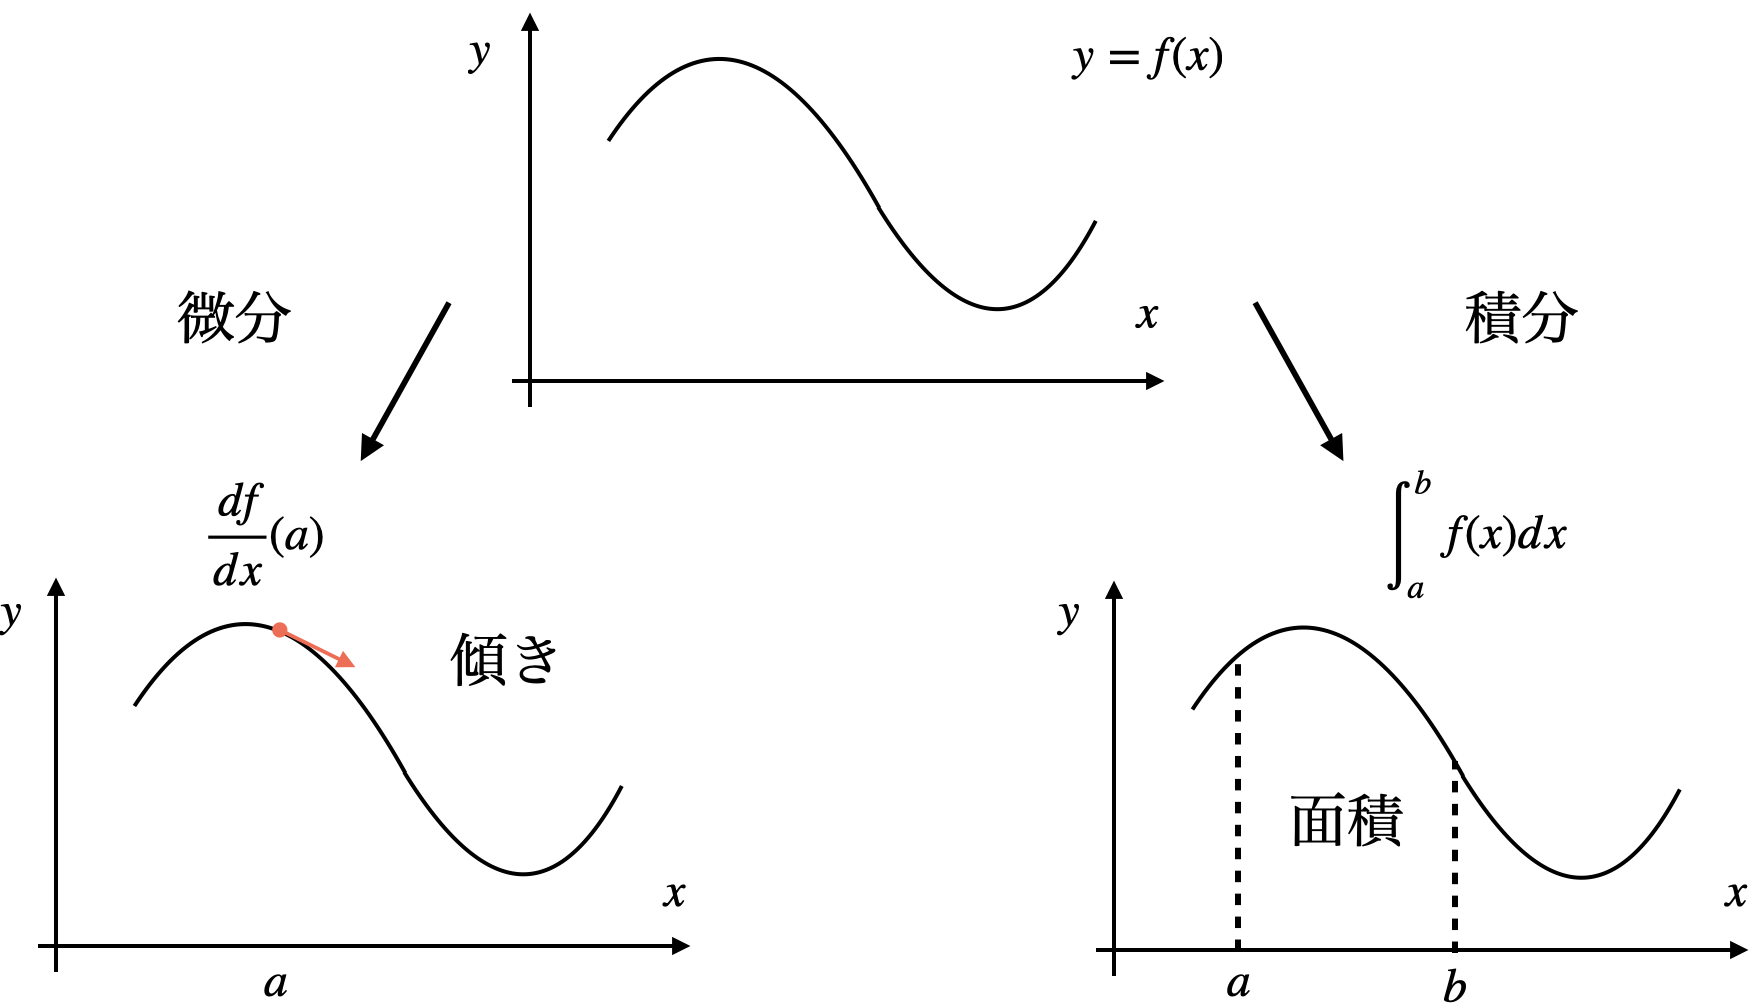
\includegraphics[width=100mm]{calculus1/diff_int.png}
 \end{center}
\end{figure}

\end{frame}


%%%%%%%%%%%%%%%%%%%%%%%%%%%%%%%%%%%%%%%%%%%%%%%%%%%%%%%%%%%%%%%%%%%%%%%%%%%%%%%%%%%%%%%
%%%%%%%%%%%%%%%%%%%%%%%%%%%%%%%%%%%%%%%%%%%%%%%%%%%%%%%%%%%%%%%%%%%%%%%%%%%%%%%%%%%%%%%


\begin{frame}
\frametitle{微分}

微分: 最も値の大きい・小さいところを探す方法

 \begin{figure}[htbp]
 \begin{center} 
  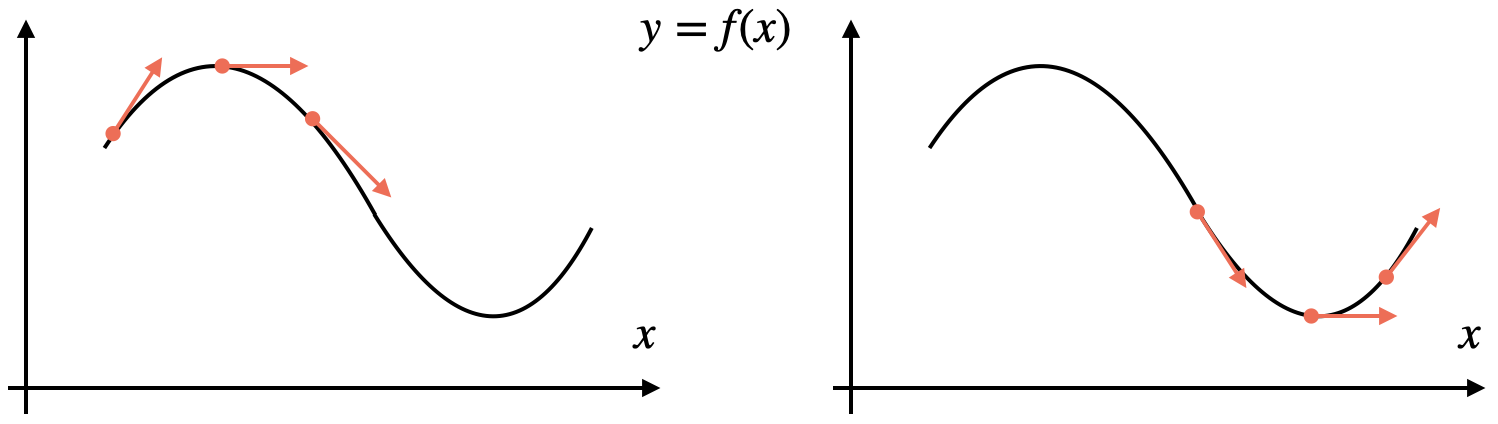
\includegraphics[width=100mm]{calculus1/diff.png}
 \end{center}
\end{figure}


\begin{itemize}
\item 極大点の頂上の手前では坂は上がり, 先では下る. 
\item 極小点の底の手前では坂は下り, 先では上がる. 
\item 極大点, 極小点 $\Rightarrow$ 傾き0. 
\item グラフの傾き = 関数の値の変化率, 未来の判断材料. 
\end{itemize}

\end{frame}


%%%%%%%%%%%%%%%%%%%%%%%%%%%%%%%%%%%%%%%%%%%%%%%%%%%%%%%%%%%%%%%%%%%%%%%%%%%%%%%%%%%%%%%
%%%%%%%%%%%%%%%%%%%%%%%%%%%%%%%%%%%%%%%%%%%%%%%%%%%%%%%%%%%%%%%%%%%%%%%%%%%%%%%%%%%%%%%


\begin{frame}
\frametitle{応用}   

最適化問題: 適当な条件を満たす最適解を探す

\begin{itemize}
\item 等周問題: 周の長さが$l$の長方形の中で面積を最大にするものは? 
\item 面積$A(x)=x(l/2-x)$
\end{itemize}

 \begin{figure}[htbp]
 \begin{center} 
  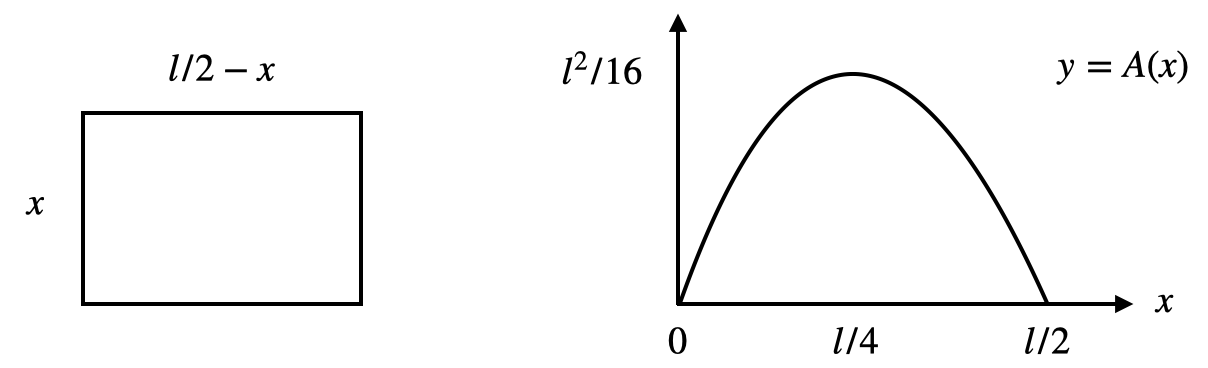
\includegraphics[width=100mm]{calculus1/LecArea.png}
 \end{center}
\end{figure}

\end{frame}


%%%%%%%%%%%%%%%%%%%%%%%%%%%%%%%%%%%%%%%%%%%%%%%%%%%%%%%%%%%%%%%%%%%%%%%%%%%%%%%%%%%%%%%
%%%%%%%%%%%%%%%%%%%%%%%%%%%%%%%%%%%%%%%%%%%%%%%%%%%%%%%%%%%%%%%%%%%%%%%%%%%%%%%%%%%%%%%


\begin{frame}
\frametitle{積分}

積分: これまでの蓄積を計算する方法

 \begin{figure}[htbp]
 \begin{center} 
  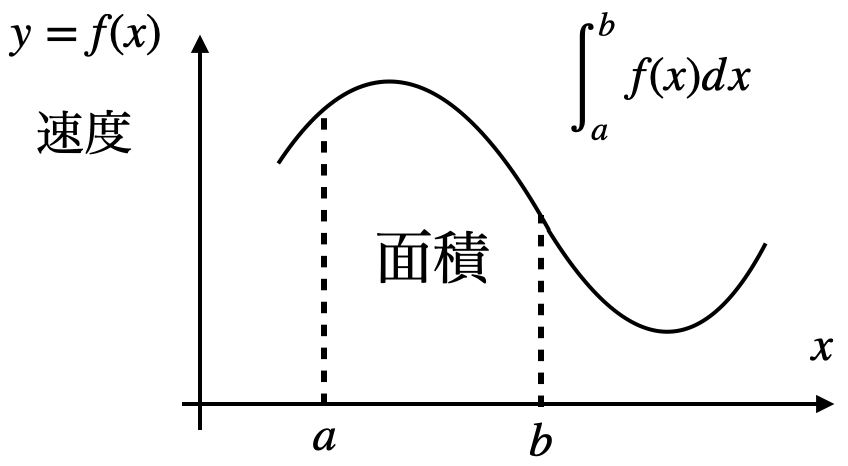
\includegraphics[width=60mm]{calculus1/int_speed.png}
 \end{center}
\end{figure}


\begin{itemize}
\item 面積$\int_a^b f(x)dx$は時刻$a$から時刻$b$までに移動した距離. 
\item 平均速度 = 面積/時間. 
\item 面積 = 過去の蓄積, 過去の判断材料.
\end{itemize}

\end{frame}


%%%%%%%%%%%%%%%%%%%%%%%%%%%%%%%%%%%%%%%%%%%%%%%%%%%%%%%%%%%%%%%%%%%%%%%%%%%%%%%%%%%%%%%
%%%%%%%%%%%%%%%%%%%%%%%%%%%%%%%%%%%%%%%%%%%%%%%%%%%%%%%%%%%%%%%%%%%%%%%%%%%%%%%%%%%%%%%


\begin{frame}
\frametitle{積分}

時刻$a$から時刻$t$までに移動した距離は$F(t)=\int_a^tf(x)dx$で与えられた. 

 \begin{figure}[htbp]
 \begin{center} 
  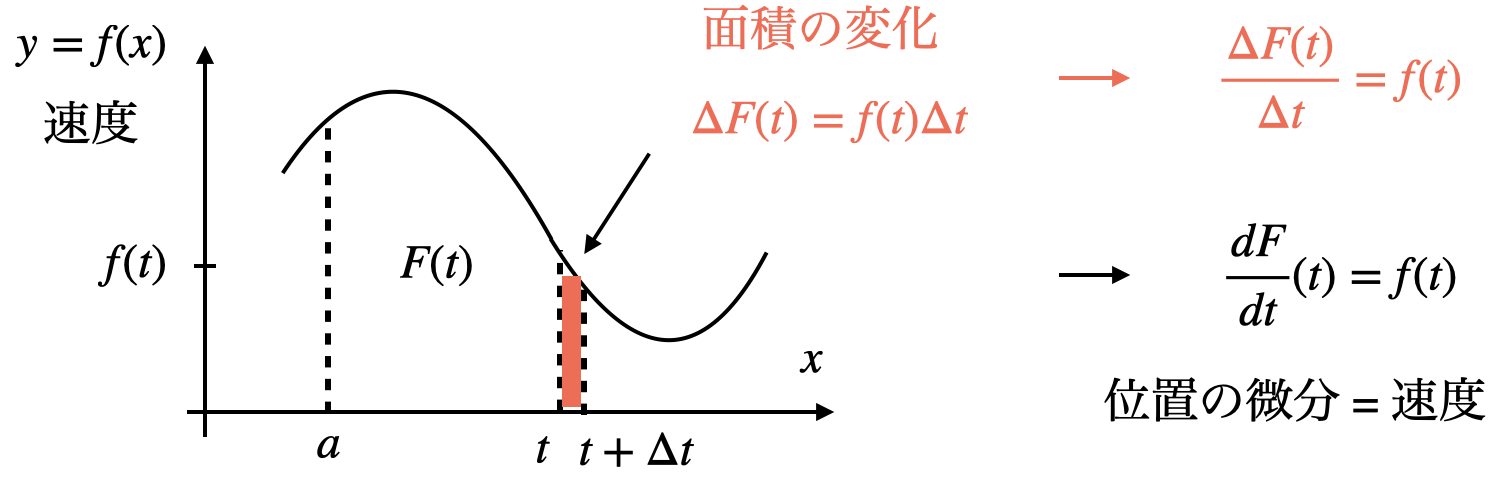
\includegraphics[width=100mm]{calculus1/diff_pos=speed.png}
 \end{center}
\end{figure}


\begin{itemize}
\item 「速度」を積分すると「位置」(過去の蓄積). 
\item 「位置」を微分すると「速度」(現在の変化). 
\item  一般に, 微分と積分は逆操作. 
\end{itemize}

\end{frame}



%%%%%%%%%%%%%%%%%%%%%%%%%%%%%%%%%%%%%%%%%%%%%%%%%%%%%%%%%%%%%%%%%%%%%%%%%%%%%%%%%%%%%%%
%%%%%%%%%%%%%%%%%%%%%%%%%%%%%%%%%%%%%%%%%%%%%%%%%%%%%%%%%%%%%%%%%%%%%%%%%%%%%%%%%%%%%%%



\begin{frame}
\frametitle{微分・積分}

以上を簡単にまとめると

 \begin{figure}[htbp]
 \begin{center} 
  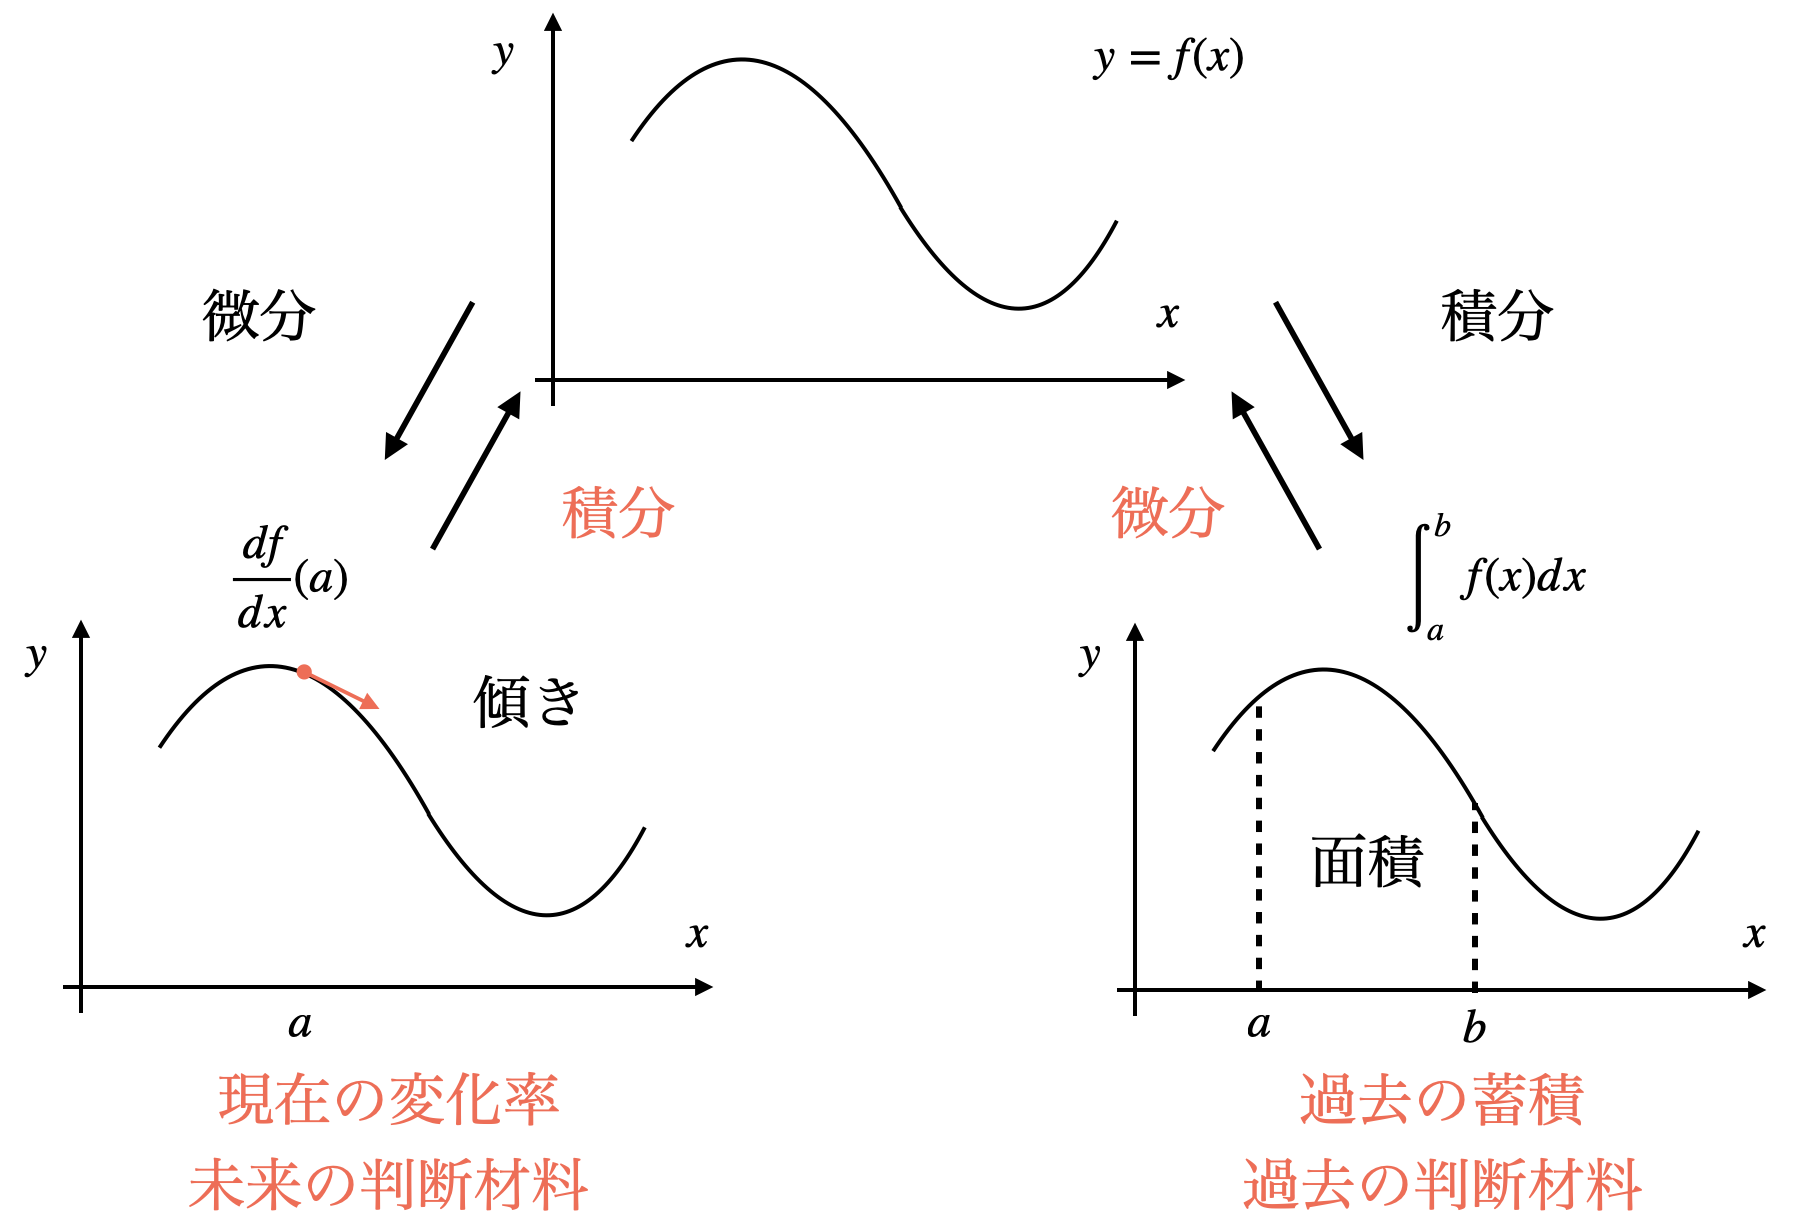
\includegraphics[width=100mm]{calculus1/diff_int2.png}
 \end{center}
\end{figure}

\end{frame}
\begin{slide}{課題\#1}
\begin{itemize}
\item 微分・積分が今後自分のキャリアにどのように役立ちそうか、今日の講義も踏まえて、考えを述べなさい。もしどうしても考えているキャリアに役立つと思えない場合には、その理由をまとめること
\item 授業に関する期待や要望などがあれば、それも含めること。採点対象外。
\item A4 1枚以内。PDFでKLMSに提出。
\end{itemize}

\end{slide}




\graphicspath{calculus1}
\section{講義概要}

\begin{frame}
\frametitle{講義概要}   

\underline{講義概要} \\
\ \\

微分・積分の基礎事項に関して講義する. 
微分は対象の変化を, 積分は対象の累積を解析する理論であり, データサイエンス, 経済学, 理工学など幅広い分野で基礎となる. 
実際, その強力な手法と幅広い応用ゆえ, 微分・積分は線形代数と合わせて大学数学の2本柱と位置付けられることが多い. 
本講義では, 一変数関数の微分・積分, 多項式近似, 多変数関数の微分・積分などを学習する. 



%\begin{enumerate}
%\item 関数, 極限, 微分, 接線, 極値問題, ..
%\item 高次微分, Taylor展開, 偏微分, ..
%\item 積分, 不定積分, 重積分, ..
%\end{enumerate}

%講義に\underline{計算用紙}と\underline{ペン}を持ってきて下さい!!

\end{frame}


%%%%%%%%%%%%%%%%%%%%%%%%%%%%%%%%%%%%%%%%%%%%%%%%%%%%%%%%%%%%%%%%%%%%%%%%%%%%%%%%%%%%%%%
%%%%%%%%%%%%%%%%%%%%%%%%%%%%%%%%%%%%%%%%%%%%%%%%%%%%%%%%%%%%%%%%%%%%%%%%%%%%%%%%%%%%%%%

%\begin{frame}
%\frametitle{参考書・成績評価・連絡先}  
%
%
%\underline{参考書} \\
%SOLにスライドをアップする.  
%自習用に参考書を一冊持っていると便利ですが, 必要ではありません. 
%例えば, 次のような教科書があります: 
%\begin{itemize}
%\item 志賀浩二, 微分・積分30講 (数学30講シリーズ), 朝倉書店. 
%\item 志賀浩二, 解析入門30講 (数学30講シリーズ), 朝倉書店. 
%\item 杉浦光夫, 解析入門I(基礎数学2), 東京大学出版会. 
%\end{itemize}
%\ \\
%
%
%\underline{成績評価} \\
%レポート2回60点 + 期末試験40点 \\
%(演習問題は提出不要) \\
%\ \\
%
%
%\underline{連絡先} \\
%atsushik@sfc.keio.ac.jp
%
%\end{frame}



%%%%%%%%%%%%%%%%%%%%%%%%%%%%%%%%%%%%%%%%%%%%%%%%%%%%%%%%%%%%%%%%%%%%%%%%%%%%%%%%%%%%%%%
%%%%%%%%%%%%%%%%%%%%%%%%%%%%%%%%%%%%%%%%%%%%%%%%%%%%%%%%%%%%%%%%%%%%%%%%%%%%%%%%%%%%%%%



\begin{frame}
\frametitle{今日の内容}



\begin{enumerate}
\item 微分・積分の概要
\item 集合, 写像
\end{enumerate}


\end{frame}




%%%%%%%%%%%%%%%%%%%%%%%%%%%%%%%%%%%%%%%%%%%%%%%%%%%%%%%%%%%%%%%%%%%%%%%%%%%%%%%%%%%%%%%
%%%%%%%%%%%%%%%%%%%%%%%%%%%%%%%%%%%%%%%%%%%%%%%%%%%%%%%%%%%%%%%%%%%%%%%%%%%%%%%%%%%%%%%

\section{微分・積分とは何か?}


\begin{frame}
\frametitle{微分・積分とは何か?}


 \begin{figure}[htbp]
 \begin{center} 
  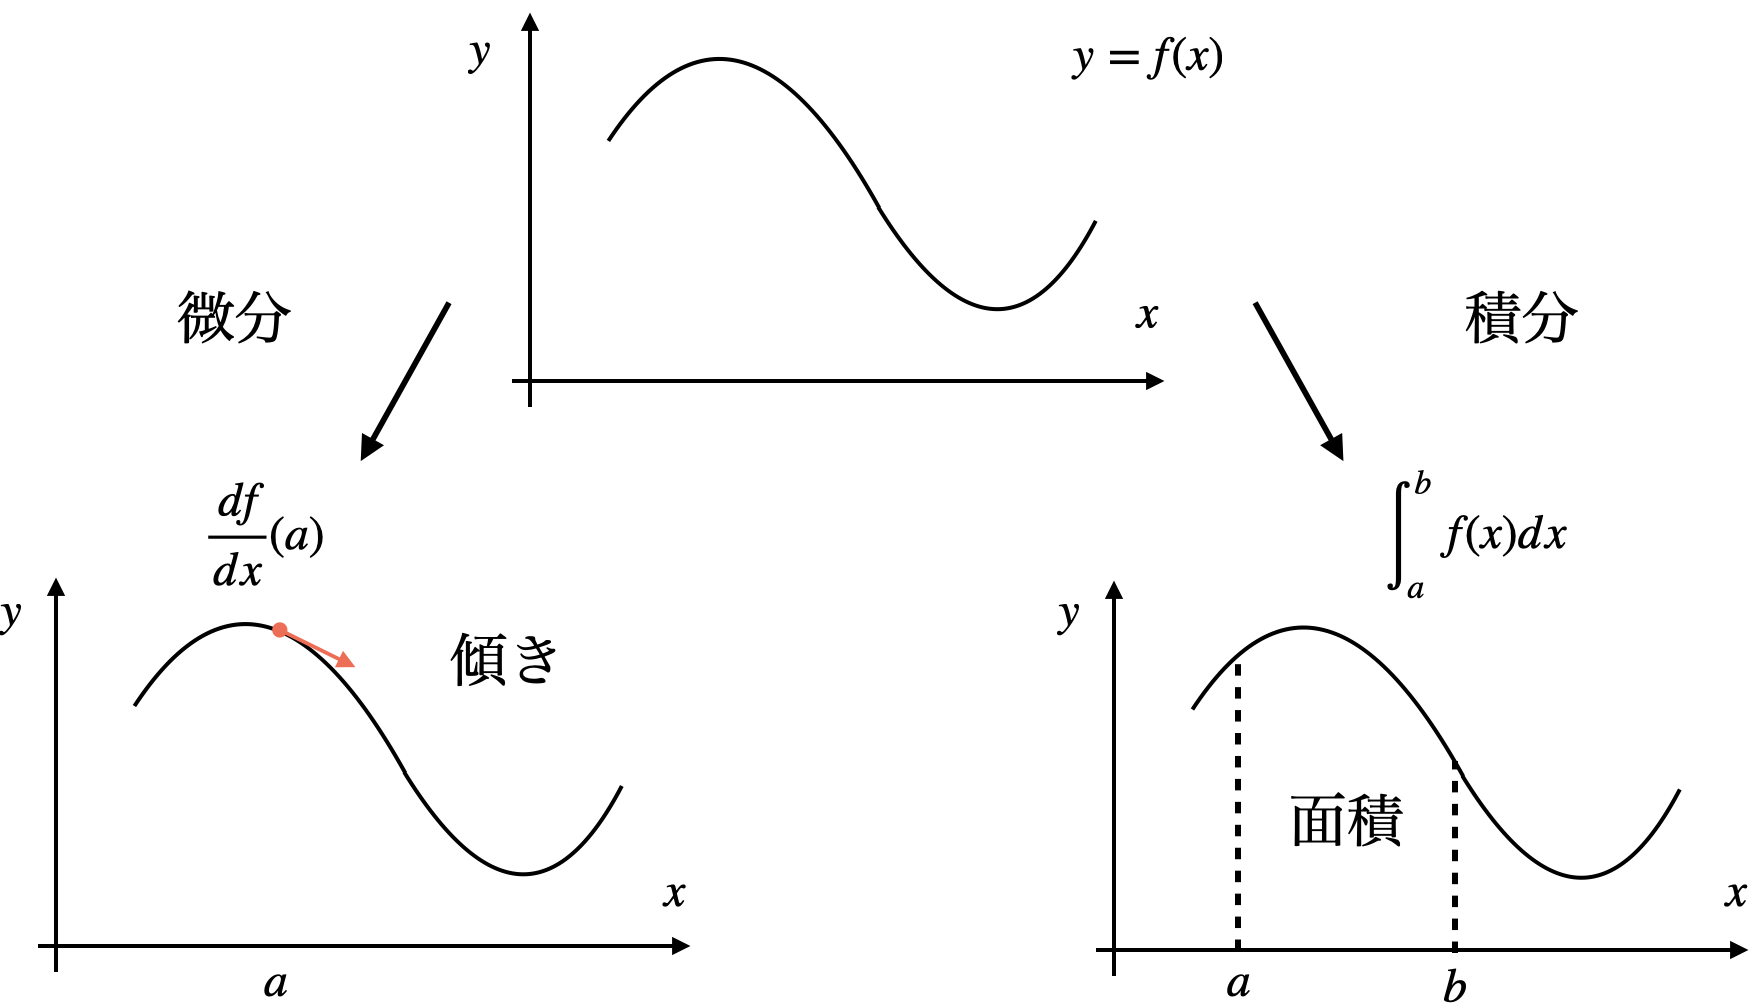
\includegraphics[width=100mm]{calculus1/diff_int.png}
 \end{center}
\end{figure}

\end{frame}


%%%%%%%%%%%%%%%%%%%%%%%%%%%%%%%%%%%%%%%%%%%%%%%%%%%%%%%%%%%%%%%%%%%%%%%%%%%%%%%%%%%%%%%
%%%%%%%%%%%%%%%%%%%%%%%%%%%%%%%%%%%%%%%%%%%%%%%%%%%%%%%%%%%%%%%%%%%%%%%%%%%%%%%%%%%%%%%


\begin{frame}
\frametitle{微分}

微分: 最も値の大きい・小さいところを探す方法

 \begin{figure}[htbp]
 \begin{center} 
  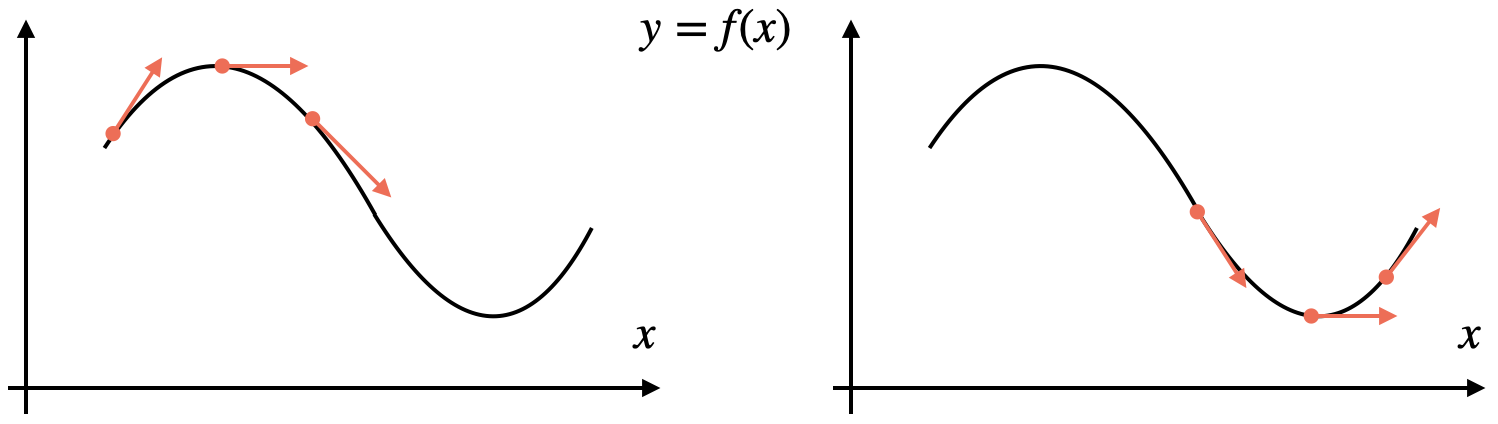
\includegraphics[width=100mm]{calculus1/diff.png}
 \end{center}
\end{figure}


\begin{itemize}
\item 極大点の頂上の手前では坂は上がり, 先では下る. 
\item 極小点の底の手前では坂は下り, 先では上がる. 
\item 極大点, 極小点 $\Rightarrow$ 傾き0. 
\item グラフの傾き = 関数の値の変化率, 未来の判断材料. 
\end{itemize}

\end{frame}


%%%%%%%%%%%%%%%%%%%%%%%%%%%%%%%%%%%%%%%%%%%%%%%%%%%%%%%%%%%%%%%%%%%%%%%%%%%%%%%%%%%%%%%
%%%%%%%%%%%%%%%%%%%%%%%%%%%%%%%%%%%%%%%%%%%%%%%%%%%%%%%%%%%%%%%%%%%%%%%%%%%%%%%%%%%%%%%


\begin{frame}
\frametitle{応用}   

最適化問題: 適当な条件を満たす最適解を探す

\begin{itemize}
\item 等周問題: 周の長さが$l$の長方形の中で面積を最大にするものは? 
\item 面積$A(x)=x(l/2-x)$
\end{itemize}

 \begin{figure}[htbp]
 \begin{center} 
  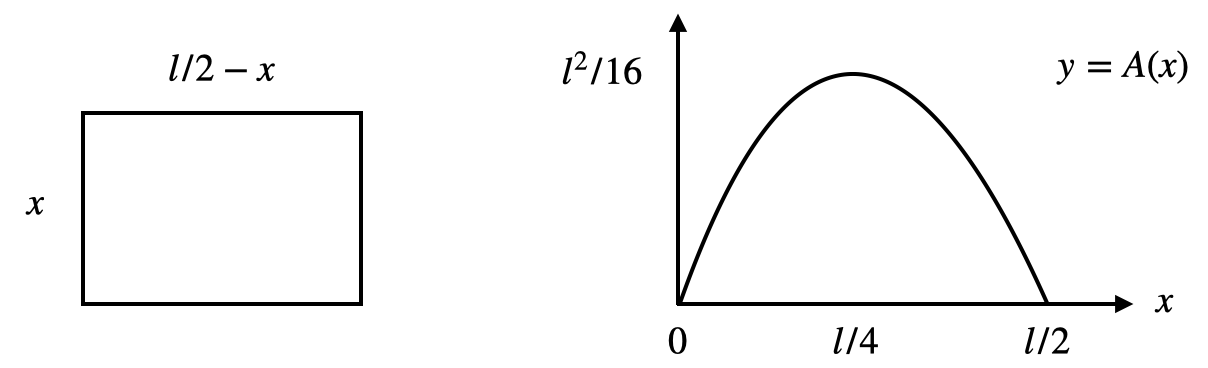
\includegraphics[width=100mm]{calculus1/LecArea.png}
 \end{center}
\end{figure}

\end{frame}


%%%%%%%%%%%%%%%%%%%%%%%%%%%%%%%%%%%%%%%%%%%%%%%%%%%%%%%%%%%%%%%%%%%%%%%%%%%%%%%%%%%%%%%
%%%%%%%%%%%%%%%%%%%%%%%%%%%%%%%%%%%%%%%%%%%%%%%%%%%%%%%%%%%%%%%%%%%%%%%%%%%%%%%%%%%%%%%


\begin{frame}
\frametitle{積分}

積分: これまでの蓄積を計算する方法

 \begin{figure}[htbp]
 \begin{center} 
  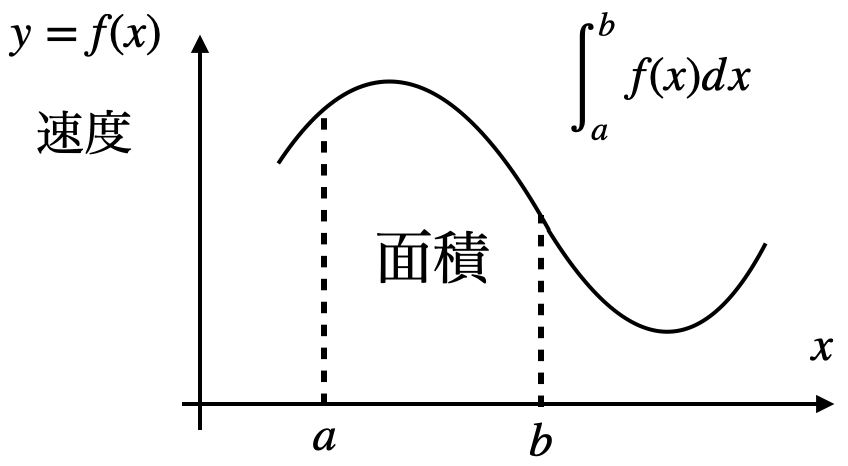
\includegraphics[width=60mm]{calculus1/int_speed.png}
 \end{center}
\end{figure}


\begin{itemize}
\item 面積$\int_a^b f(x)dx$は時刻$a$から時刻$b$までに移動した距離. 
\item 平均速度 = 面積/時間. 
\item 面積 = 過去の蓄積, 過去の判断材料.
\end{itemize}

\end{frame}


%%%%%%%%%%%%%%%%%%%%%%%%%%%%%%%%%%%%%%%%%%%%%%%%%%%%%%%%%%%%%%%%%%%%%%%%%%%%%%%%%%%%%%%
%%%%%%%%%%%%%%%%%%%%%%%%%%%%%%%%%%%%%%%%%%%%%%%%%%%%%%%%%%%%%%%%%%%%%%%%%%%%%%%%%%%%%%%


\begin{frame}
\frametitle{積分}

時刻$a$から時刻$t$までに移動した距離は$F(t)=\int_a^tf(x)dx$で与えられた. 

 \begin{figure}[htbp]
 \begin{center} 
  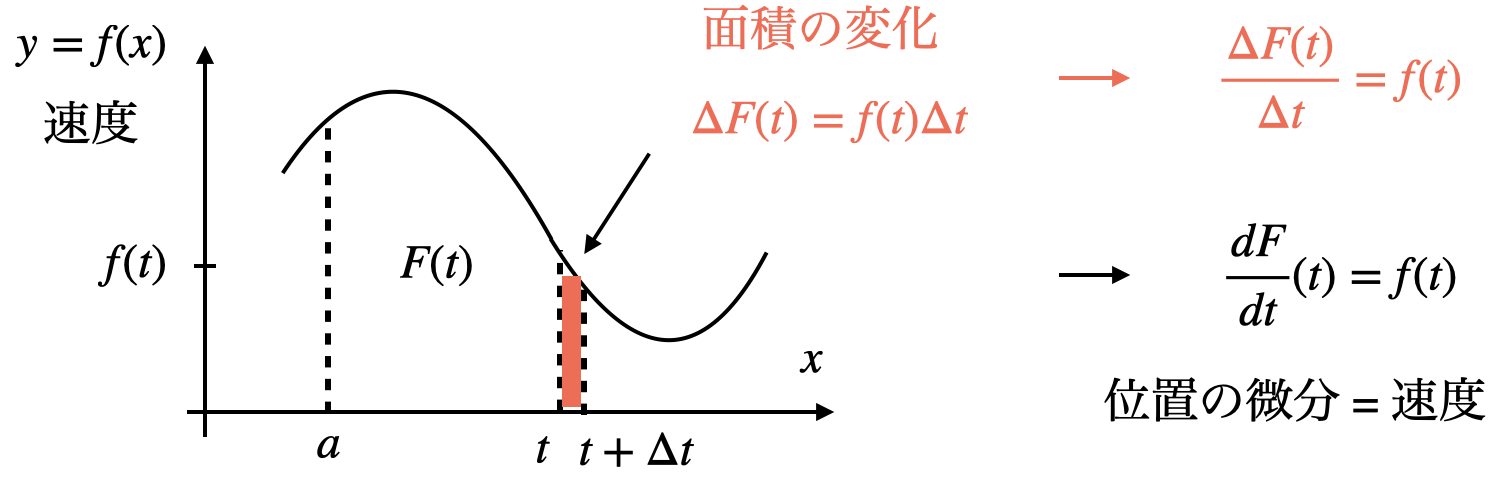
\includegraphics[width=100mm]{calculus1/diff_pos=speed.png}
 \end{center}
\end{figure}


\begin{itemize}
\item 「速度」を積分すると「位置」(過去の蓄積). 
\item 「位置」を微分すると「速度」(現在の変化). 
\item  一般に, 微分と積分は逆操作. 
\end{itemize}

\end{frame}



%%%%%%%%%%%%%%%%%%%%%%%%%%%%%%%%%%%%%%%%%%%%%%%%%%%%%%%%%%%%%%%%%%%%%%%%%%%%%%%%%%%%%%%
%%%%%%%%%%%%%%%%%%%%%%%%%%%%%%%%%%%%%%%%%%%%%%%%%%%%%%%%%%%%%%%%%%%%%%%%%%%%%%%%%%%%%%%



\begin{frame}
\frametitle{微分・積分}

以上を簡単にまとめると

 \begin{figure}[htbp]
 \begin{center} 
  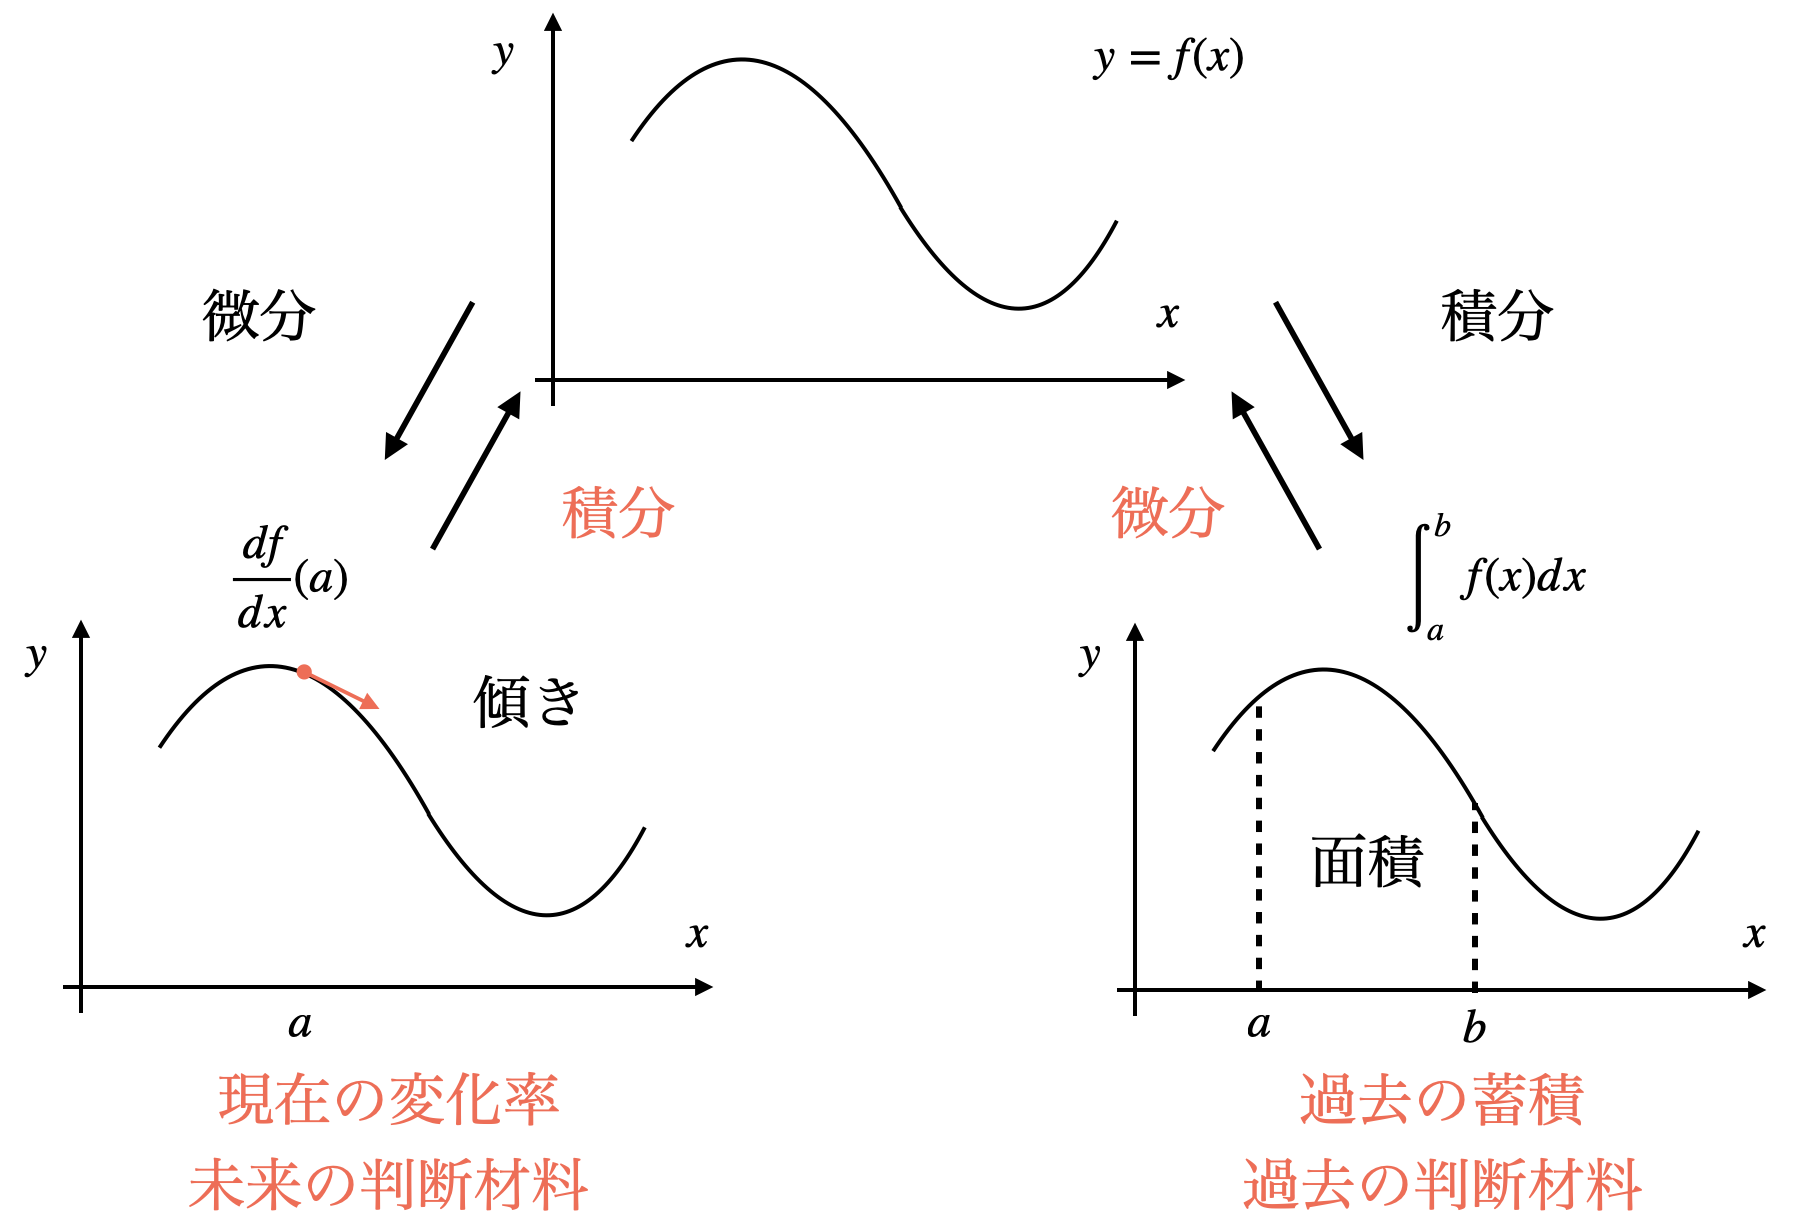
\includegraphics[width=100mm]{calculus1/diff_int2.png}
 \end{center}
\end{figure}

\end{frame}






%%%%%%%%%%%%%%%%%%%%%%%%%%%%%%%%%%%%%%%%%%%%%%%%%%%%%%%%%%%%%%%%%%%%%%%%%%%%%%%%%%%%%%%
%%%%%%%%%%%%%%%%%%%%%%%%%%%%%%%%%%%%%%%%%%%%%%%%%%%%%%%%%%%%%%%%%%%%%%%%%%%%%%%%%%%%%%%
%%%%%%%%%%%%%%%%%%%%%%%%%%%%%%%%%%%%%%%%%%%%%%%%%%%%%%%%%%%%%%%%%%%%%%%%%%%%%%%%%%%%%%%
%%%%%%%%%%%%%%%%%%%%%%%%%%%%%%%%%%%%%%%%%%%%%%%%%%%%%%%%%%%%%%%%%%%%%%%%%%%%%%%%%%%%%%%


\section{集合論}

\begin{frame}
\frametitle{集合, 濃度}   

記号の準備も兼ねて, 集合論から始める. 

\begin{Def}
\begin{itemize}
\item 
対象(もの)の集まりを\underline{集合}という. 
対象となるものは, 数字, 記号, 文字列など色々考えられる. 
%ただし, その集まりに含まれるかどうか明確に識別できなければならない. 
\item
集合の構成要素を\underline{元}(要素)という. 
$a$が集合$A$の元であることを, $a \in A$と表す. 
$a$が$A$の元であるとき, $a$は$A$に含まれるということもある. 
$a \in A$の否定を$a \notin A$と書く. 
\item 
集合$A$の元の数を$|A|$で表し, $A$の\underline{濃度}(位数)と呼ぶ. 
集合$A$で
\begin{itemize}
\item $|A|=\infty$なるものは\underline{無限集合}, 
\item $|A| \ne \infty$なるものは\underline{有限集合}. 
\end{itemize}
\end{itemize}
\end{Def}


\end{frame}

%%%%%%%%%%%%%%%%%%%%%%%%%%%%%%%%%%%%%%%%%%%%%%%%%%%%%%%%%%%%%%%%%%%%%%%%%%%%%%%%%%%%%%%
%%%%%%%%%%%%%%%%%%%%%%%%%%%%%%%%%%%%%%%%%%%%%%%%%%%%%%%%%%%%%%%%%%%%%%%%%%%%%%%%%%%%%%%



\begin{frame}
\frametitle{集合}   

\begin{Ex}
\begin{enumerate}
%\item 整数$1, 3, 5, 7$を元に持つ集合$A=\{1,3,5,7\}$に関して, $1\in A$であるが$2 \notin A$である. 
%また$|A|=4$であるから, $A$は有限集合. 
\item $A=\{\text{りんご, みかん, バナナ}\}$とすれば, $\text{みかん} \in A$. 
\item 都道府県の集合
$$
A=\{\text{北海道, 青森県, 岩手県, 宮城県, \dots}\}
$$
は$|A|=47$. 
\item 
\begin{itemize}
\item $\N=\{1,2,3,\dots\}$:自然数, 
\item $\Z=\{ \dots, -2,-1,0,1,2,\dots \}$:整数, 
\item $\Q$:有理数(分数全体), $\R$:実数
\end{itemize}
これらは全て無限集合. 
\end{enumerate} 
\end{Ex}



\end{frame}



%%%%%%%%%%%%%%%%%%%%%%%%%%%%%%%%%%%%%%%%%%%%%%%%%%%%%%%%%%%%%%%%%%%%%%%%%%%%%%%%%%%%%%%
%%%%%%%%%%%%%%%%%%%%%%%%%%%%%%%%%%%%%%%%%%%%%%%%%%%%%%%%%%%%%%%%%%%%%%%%%%%%%%%%%%%%%%%


\begin{frame}
\frametitle{外延的記法} 

集合を定義するには, その集合に含まれる元を指定すれば良い. \\
\ \\

\underline{外延的記法}: その集合が持つ元を全て列挙する直接的な方法. 例えば
$$
\{1,2,3,4\}, \ \{\text{子豚, 狸, 狐, 猫}\}, \ \{1,3,5,7,9,11,\dots\}. 
$$
最後の集合は奇数全体の集合を意図したものだが, 「$\dots$」に何が並ぶのかが明確でないと誤解を招く恐れがある. 


\begin{Ex}
自然数の集合
$$
\N=\{1,2,3,4,5,\dots\}. 
$$
整数の集合
$$
\Z=\{\dots, -2,-1,0,1,2,\dots\}. 
$$
\end{Ex}

\end{frame}

%%%%%%%%%%%%%%%%%%%%%%%%%%%%%%%%%%%%%%%%%%%%%%%%%%%%%%%%%%%%%%%%%%%%%%%%%%%%%%%%%%%%%%%
%%%%%%%%%%%%%%%%%%%%%%%%%%%%%%%%%%%%%%%%%%%%%%%%%%%%%%%%%%%%%%%%%%%%%%%%%%%%%%%%%%%%%%%


\begin{frame}
\frametitle{内包的記法}   

 \underline{内包的記法}: 集合に含まれる元の条件を明示する方法. 
「命題$P$が真となる$x \in X$全体の集合」を
$$
\{ x \in X \ | \ P\}
$$
と書く. 
ここで$X$は変数$x$が動く範囲の集合である.  
例えば
$$
\{n \in \Z \ | \ -1.4 \le n \le 3\}
$$
は「整数$n$であって$-1.4 \le n \le 3$が成立するもの全体の集合」と読む. 
外延的方法を用いれば, これは
$$
\{-1,0,1,2,3\}
$$
とも表せる. 

\end{frame}



%%%%%%%%%%%%%%%%%%%%%%%%%%%%%%%%%%%%%%%%%%%%%%%%%%%%%%%%%%%%%%%%%%%%%%%%%%%%%%%%%%%%%%%
%%%%%%%%%%%%%%%%%%%%%%%%%%%%%%%%%%%%%%%%%%%%%%%%%%%%%%%%%%%%%%%%%%%%%%%%%%%%%%%%%%%%%%%


\begin{frame}
\frametitle{外延的方法 vs 内包的記法}   

\begin{Ex}
実数$a<b$に対して, $a,b$を端点とする閉区間, 開区間が
\begin{align*}
[a,b] = \{x \in \R \ | \ a \le x \le b \}, \ \ (a,b) &=\{x \in \R \ | \ a < x < b \} 
\end{align*}
で定義される. 
同様に半開区間
\begin{align*}
(a,b] = \{x \in \R \ | \ a < x \le b \}, \ \ [a,b) &=\{x \in \R \ | \ a \le x < b \}
\end{align*}
が定義される. 
これらは外延的方法では記述できない無限集合である. 
\end{Ex}

2つの黒丸に挟まれた区間が閉空間, 2つの白丸に挟まれた区間が開空間: 
 \begin{figure}[htbp]
 \begin{center} 
  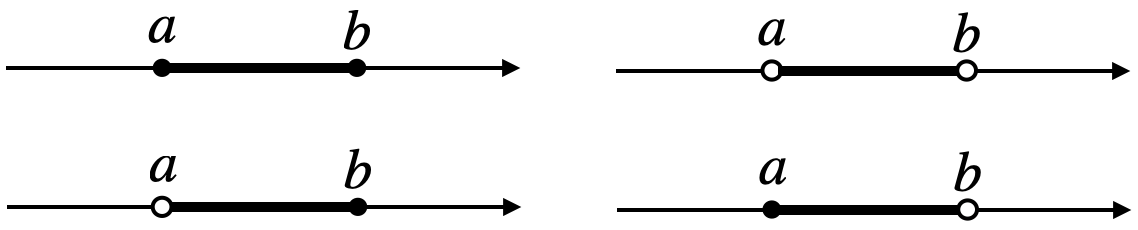
\includegraphics[width=80mm]{calculus1/interval.png}
 \end{center}
\end{figure}

\end{frame}




%%%%%%%%%%%%%%%%%%%%%%%%%%%%%%%%%%%%%%%%%%%%%%%%%%%%%%%%%%%%%%%%%%%%%%%%%%%%%%%%%%%%%%%
%%%%%%%%%%%%%%%%%%%%%%%%%%%%%%%%%%%%%%%%%%%%%%%%%%%%%%%%%%%%%%%%%%%%%%%%%%%%%%%%%%%%%%%


\begin{frame}
\frametitle{直積集合}   

\begin{Def}[直積集合]
$A, B$を集合とする. 
$a \in A$と$b \in B$を並べた$(a,b)$を\underline{順序対}という. 
順序対全体のなす集合を$A$と$B$の\underline{直積集合}といい, $A \times B$と書く. 
$$
A \times B = \{(a,b) \ | \ a \in A, \ b \in B\}. 
$$
\end{Def}

$A=\{a,b\}, B=\{c,d\}$とすれば
\begin{align}
A\times B &= \{(x,y) \ | \ x \in A, \ y \in B \} \notag \\
&=\{(a,c), (a,d), (b,c), (b,d)\}.  \notag
\end{align}

同様に3つの集合$A,B,C$の直積集合$A \times B \times C$や, $n$個の集合$A_1,\dots,A_n$の直積集合
$$
A_1 \times \dots \times A_n
$$
が定義される. 



\end{frame}



%%%%%%%%%%%%%%%%%%%%%%%%%%%%%%%%%%%%%%%%%%%%%%%%%%%%%%%%%%%%%%%%%%%%%%%%%%%%%%%%%%%%%%%
%%%%%%%%%%%%%%%%%%%%%%%%%%%%%%%%%%%%%%%%%%%%%%%%%%%%%%%%%%%%%%%%%%%%%%%%%%%%%%%%%%%%%%%



\begin{frame}
\frametitle{$n$次元座標空間$\R^n$}   


\begin{Ex}
\begin{itemize}
\item 実数全体の集合$\R$は実直線$\R^1$と同一視することができた. 
\item 実平面
$$
\R^2=\R \times \R=\{(x,y) \ | \ x \in \R, \ y \in \R\}
$$
\item $3$次元座標空間
$$
\R^3=\R \times \R \times \R=\{(x,y,z) \ | \ x \in \R, \ y \in \R \ z\in \R\}
$$
\item 一般に, $\R^n$は$n$次元座標空間, もしくは$n$次元ユークリッド空間と呼ばれる. 
\end{itemize}
\end{Ex}

この講義では主に$\R, \R^2,\R^3$を扱う. 

\end{frame}

%%%%%%%%%%%%%%%%%%%%%%%%%%%%%%%%%%%%%%%%%%%%%%%%%%%%%%%%%%%%%%%%%%%%%%%%%%%%%%%%%%%%%%%
%%%%%%%%%%%%%%%%%%%%%%%%%%%%%%%%%%%%%%%%%%%%%%%%%%%%%%%%%%%%%%%%%%%%%%%%%%%%%%%%%%%%%%%


%\begin{frame}
%\frametitle{直積集合}   
%
%\begin{Ex}
%必ずしも同じような集合の直積を取る必要はない. 
%例えば
%$$
%A=\{\text{りんご, みかん, バナナ}\}, \ \ \ B=\{-3,7\}
%$$
%とすれば, $A\times B$は
%\begin{align}
%&\{(\text{りんご},-3), (\text{みかん},-3), (\text{バナナ},-3), \notag \\
%& \ \ \ (\text{りんご},7),  (\text{みかん},7), (\text{バナナ},7)\} \notag 
%\end{align}
%なる6つの元を持つ集合である. 
%\end{Ex}
%
%
%\end{frame}



%%%%%%%%%%%%%%%%%%%%%%%%%%%%%%%%%%%%%%%%%%%%%%%%%%%%%%%%%%%%%%%%%%%%%%%%%%%%%%%%%%%%%%%
%%%%%%%%%%%%%%%%%%%%%%%%%%%%%%%%%%%%%%%%%%%%%%%%%%%%%%%%%%%%%%%%%%%%%%%%%%%%%%%%%%%%%%%


\begin{frame}
\frametitle{包含関係}   


複数の集合があるとき, それらの間の関係を考えることは自然である.  
最も基本的なものが\underline{包含関係}である.

\begin{Def}[部分集合]
$A, B$を集合とする.
\begin{enumerate}
\item 任意の$A$の元が$B$の元でもあるとき, $A$は$B$の\underline{部分集合}であるといい, $A \subset B$と書く.  
%すなわち, $A \subset B$であるとは, $x \in A \Rightarrow x \in B$が成立することである. 
$A \subset B$でないとき, $A \not\subset B$と書く.
\item $A \subset B$かつ$B \subset A$のとき, $A$と$B$は\underline{(集合として)等しい}といい, $A=B$と書く. 
\item $A \subset B$かつ$A \ne B$ のとき, $A$は$B$の\underline{真部分集合}であるといい, $A \subsetneq B$とかく.
\end{enumerate} 
\end{Def}


\end{frame}


%%%%%%%%%%%%%%%%%%%%%%%%%%%%%%%%%%%%%%%%%%%%%%%%%%%%%%%%%%%%%%%%%%%%%%%%%%%%%%%%%%%%%%%
%%%%%%%%%%%%%%%%%%%%%%%%%%%%%%%%%%%%%%%%%%%%%%%%%%%%%%%%%%%%%%%%%%%%%%%%%%%%%%%%%%%%%%%


\begin{frame}
\frametitle{包含関係}   

人間の集合を$\{\text{人間}\}$と略記したりする. 
これは人間1人からなる集合ではない. 

\begin{Ex}
\begin{enumerate}
\item $\{\text{人間}\} \subset \{\text{哺乳類}\}$, $\{\text{犬}\} \subset \{\text{哺乳類}\}$
\item $\N \subset \Z \subset \Q \subset  \R$
\item 実数$a<b$に対して, $(a,b) \subsetneq [a,b]$である. 
一方で, $(a,b]$と$[a,b)$の間には包含関係はない. 
\end{enumerate} 
\end{Ex}


 \begin{figure}[htbp]
 \begin{center} 
  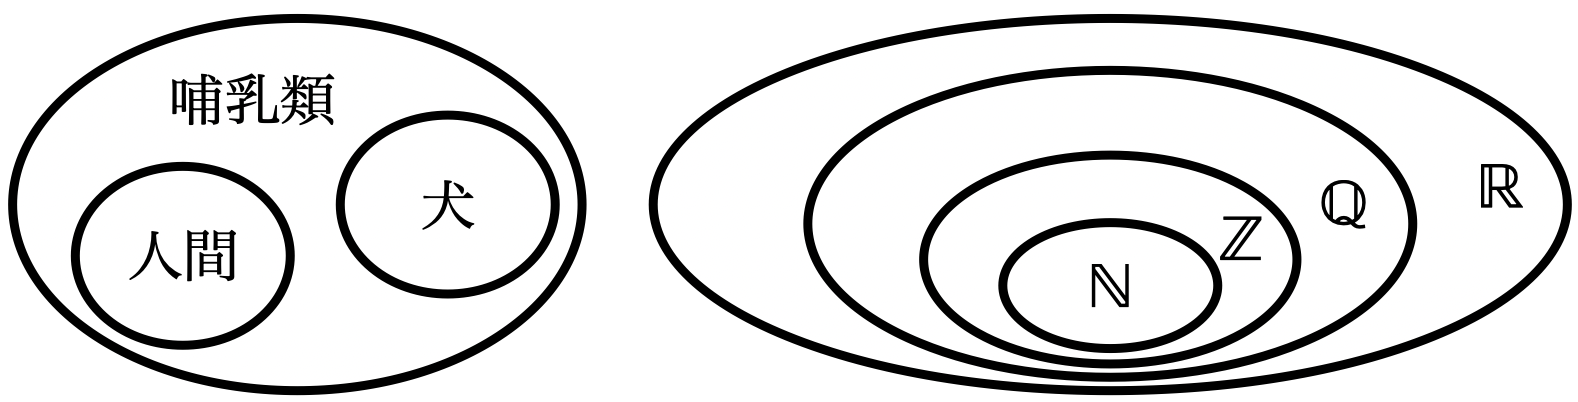
\includegraphics[width=100mm]{calculus1/subsets.png}
 \end{center}
\end{figure}

\end{frame}



%%%%%%%%%%%%%%%%%%%%%%%%%%%%%%%%%%%%%%%%%%%%%%%%%%%%%%%%%%%%%%%%%%%%%%%%%%%%%%%%%%%%%%%
%%%%%%%%%%%%%%%%%%%%%%%%%%%%%%%%%%%%%%%%%%%%%%%%%%%%%%%%%%%%%%%%%%%%%%%%%%%%%%%%%%%%%%%


%\begin{frame}
%\frametitle{空集合}   
%
%
%\begin{Def}[空集合]
%元を1つも含まない集合を\underline{空集合}といい, $\emptyset$とかく. 
%外延的方法を用いれば
%$$
%\emptyset=\{\}
%$$
%である. 
%どんな集合$A$に対しても, $\emptyset \subset A$が成立する.  
%%これは約束と思っても良いし, 次のようにして導くことも できる. 空集合は元を一つも含まないのだから, x ∈ \UTF{2205} は任意の x に対して偽である. 
%%そ こで,「x∈\UTF{2205}⇒x∈A」は真である. よって,\UTF{2205}⊂Aとなる.
%\end{Def}
%
%
%\begin{Ex}
%集合$A=\{1,2,3\}$の部分集合を全て列挙すると
%$$
%\emptyset, \{1\},\{2\},\{3\}, \{1,2\},\{2,3\},\{3,1\},\{1,2,3\} 
%$$
%の8つである. 
%\end{Ex}
%
%
%
%\end{frame}




%%%%%%%%%%%%%%%%%%%%%%%%%%%%%%%%%%%%%%%%%%%%%%%%%%%%%%%%%%%%%%%%%%%%%%%%%%%%%%%%%%%%%%%
%%%%%%%%%%%%%%%%%%%%%%%%%%%%%%%%%%%%%%%%%%%%%%%%%%%%%%%%%%%%%%%%%%%%%%%%%%%%%%%%%%%%%%%

\section{写像}

\begin{frame}
\frametitle{写像}

\begin{Def} \label{写像定義}
\begin{itemize}
\item 集合$X$の各元に対して, 集合$Y$の元を唯一つ定める対応のことを写像と呼び, $f:X \rightarrow Y$と表す. 
$X$を\underline{定義域}, $Y$を\underline{値域}という. 
\item 写像$f:X\rightarrow Y$によって$x \in X$が$y\in Y$に対応するとき, $y$を$f$による$x$の\underline{像}といい, $y=f(x)$と書く. 
この対応を次のように書く. \vspace{-1mm}
$$
f:X \longrightarrow Y, \ \ \ x \mapsto y. 
$$
\end{itemize}
\end{Def}

\vspace{-1mm}

 \begin{figure}[htbp]
 \begin{center} 
  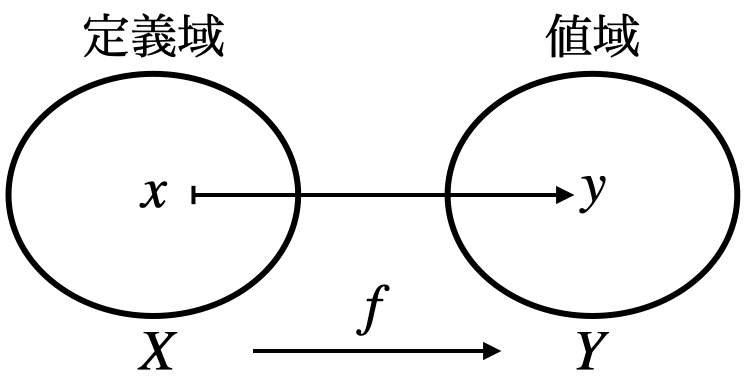
\includegraphics[width=50mm]{calculus1/map.png}
 \end{center}
\end{figure}

\vspace{-1mm}

\end{frame}


%%%%%%%%%%%%%%%%%%%%%%%%%%%%%%%%%%%%%%%%%%%%%%%%%%%%%%%%%%%%%%%%%%%%%%%%%%%%%%%%%%%%%%%
%%%%%%%%%%%%%%%%%%%%%%%%%%%%%%%%%%%%%%%%%%%%%%%%%%%%%%%%%%%%%%%%%%%%%%%%%%%%%%%%%%%%%%%




\begin{frame}
\frametitle{写像}


\begin{Ex}
\begin{enumerate}
\item $f:\{\text{人間}\} \longrightarrow \Z, \ \ \ A \mapsto \text{$A$の年齢}$
\item $g:\{\text{犬}\} \longrightarrow \R, \ \ \ A \mapsto \text{$A$の身長}$
\item $h:\{\text{猫}\} \longrightarrow \{\text{猫}\}, \ \ \ A \mapsto \text{$A$の母猫}$
\item $i:\{\text{日本の大学}\} \longrightarrow \N, \ \ \ \text{$A$大学} \mapsto \text{$A$大学の学生数}$
\item $j:\{\text{日本の大学}\} \longrightarrow \{\text{都道府県}\}, \ \ \ \text{$A$大学} \mapsto \text{$A$大学本部の所在地}$
\end{enumerate}
一方で, 人間$A$と$A$の友人の対応は写像ではない. 
$A$の友人が1人とは限らないからである. 
\end{Ex}


\end{frame}



%%%%%%%%%%%%%%%%%%%%%%%%%%%%%%%%%%%%%%%%%%%%%%%%%%%%%%%%%%%%%%%%%%%%%%%%%%%%%%%%%%%%%%%
%%%%%%%%%%%%%%%%%%%%%%%%%%%%%%%%%%%%%%%%%%%%%%%%%%%%%%%%%%%%%%%%%%%%%%%%%%%%%%%%%%%%%%%


\begin{frame}
\frametitle{像}


\begin{Def}
写像$f:X\rightarrow Y$の\underline{像}を
$$
\Imag f = \{ f(x) \ | \ x \in X\}
$$
で定義する. 
つまり$x$が$X$の全ての元を動くとき, $x$の像$f(x)$全体のなす$Y$の部分集合のことである. 
\end{Def}


 \begin{figure}[htbp]
 \begin{center} 
  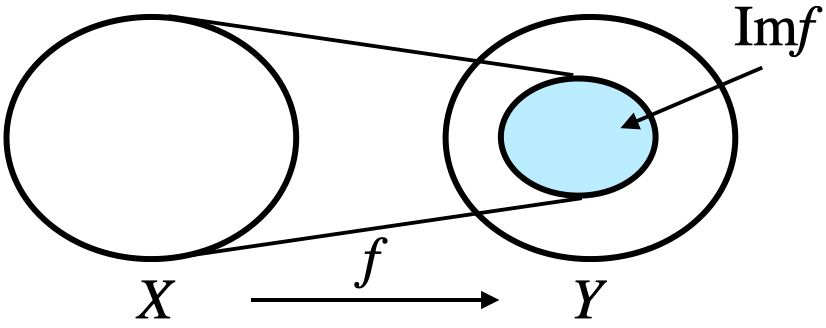
\includegraphics[width=50mm]{calculus1/imf.png}
 \end{center}
\end{figure}


\end{frame}

%%%%%%%%%%%%%%%%%%%%%%%%%%%%%%%%%%%%%%%%%%%%%%%%%%%%%%%%%%%%%%%%%%%%%%%%%%%%%%%%%%%%%%%
%%%%%%%%%%%%%%%%%%%%%%%%%%%%%%%%%%%%%%%%%%%%%%%%%%%%%%%%%%%%%%%%%%%%%%%%%%%%%%%%%%%%%%%


\begin{frame}
\frametitle{全射, 単射}


\begin{Def}$f:X\rightarrow Y$を写像とする. 
\begin{enumerate}
\item $f$が\underline{全射}であるとは$\Imag f = Y$が成立すること. 
つまり「どの$y \in Y$に対しても$x \in X$が存在して$y=f(x)$」. 
\item $f$が\underline{単射}であるとは「$x_1\ne x_2$ならば$f(x_1)\ne f(x_2)$」が成立すること. 
同値な対偶条件は「$f(x_1)= f(x_2)$ならば$x_1= x_2$」.  
\item $f$が\underline{全単射}であるとは, 全射かつ単射であること. 
\end{enumerate}
\end{Def}



\end{frame}

%%%%%%%%%%%%%%%%%%%%%%%%%%%%%%%%%%%%%%%%%%%%%%%%%%%%%%%%%%%%%%%%%%%%%%%%%%%%%%%%%%%%%%%
%%%%%%%%%%%%%%%%%%%%%%%%%%%%%%%%%%%%%%%%%%%%%%%%%%%%%%%%%%%%%%%%%%%%%%%%%%%%%%%%%%%%%%%


\begin{frame}
\frametitle{全射, 単射}

\begin{Ex}
\begin{enumerate}
\item $f:\R \rightarrow \R, x \mapsto x^2(x-1)$は(全射だが)単射ではない. 
\item $g:\R \rightarrow \R, x \mapsto x^2$は全射でも単射でもない. $\Imag g=\R_{\ge 0}$. 
\item $h:\R \rightarrow \R, x \mapsto x^3$は全単射である. 
\end{enumerate}
\end{Ex}


\begin{Prob}
次の写像は全射か? 単射か? 
\begin{enumerate}
\item $f:\Z \rightarrow \Z, x \mapsto x^2(x-1)$.  
\item $g:\Z \rightarrow \Z, x \mapsto x^2$.
\item $h:\Z \rightarrow \Z, x \mapsto x^3$. 
\end{enumerate}
\end{Prob}



\end{frame}



%%%%%%%%%%%%%%%%%%%%%%%%%%%%%%%%%%%%%%%%%%%%%%%%%%%%%%%%%%%%%%%%%%%%%%%%%%%%%%%%%%%%%%%
%%%%%%%%%%%%%%%%%%%%%%%%%%%%%%%%%%%%%%%%%%%%%%%%%%%%%%%%%%%%%%%%%%%%%%%%%%%%%%%%%%%%%%%


\begin{frame}
\frametitle{全射, 単射, 恒等写像}

\begin{Ex}
次の写像を考える: 
\begin{align*}
f: & \{\text{日本の大学}\} \longrightarrow \N, \ \ \ \text{$A$大学} \mapsto \text{$A$大学の学生数} \\
g:& \{\text{日本の大学}\} \longrightarrow \{\text{都道府県}\}, \ \ \ \text{$A$大学} \mapsto \text{$A$大学の所在地}
\end{align*}
写像$f$は全射ではない(単射であろうか?). 写像$g$は全射だが, 単射ではない. 
\end{Ex}


\begin{Ex}
何もしない写像$\id :X \rightarrow X, x \mapsto x$を\underline{恒等写像}という. 
恒等写像は全単射である. 
\end{Ex}


\end{frame}



%%%%%%%%%%%%%%%%%%%%%%%%%%%%%%%%%%%%%%%%%%%%%%%%%%%%%%%%%%%%%%%%%%%%%%%%%%%%%%%%%%%%%%%
%%%%%%%%%%%%%%%%%%%%%%%%%%%%%%%%%%%%%%%%%%%%%%%%%%%%%%%%%%%%%%%%%%%%%%%%%%%%%%%%%%%%%%%


\begin{frame}
\frametitle{全射, 単射, 恒等写像}

\begin{Prob}
次の写像は全射か? 単射か? 
\begin{enumerate}
\item 慶應義塾大学の学生に対して, 学籍番号を対応させる写像
$$
f:\{ \text{慶応義塾生}\} \longrightarrow \Z^8
$$
\item 値域を学籍番号となる番号に限ったらどうであろうか? 
$$
g:\{ \text{慶応義塾生}\} \longrightarrow \{ \text{学籍番号}\} \subset \Z^8
$$
\end{enumerate}
\end{Prob}

\end{frame}




%%%%%%%%%%%%%%%%%%%%%%%%%%%%%%%%%%%%%%%%%%%%%%%%%%%%%%%%%%%%%%%%%%%%%%%%%%%%%%%%%%%%%%%
%%%%%%%%%%%%%%%%%%%%%%%%%%%%%%%%%%%%%%%%%%%%%%%%%%%%%%%%%%%%%%%%%%%%%%%%%%%%%%%%%%%%%%%


\begin{frame}
\frametitle{合成写像}

\begin{Def}
写像$f:X \rightarrow Y, g:Y\rightarrow Z$に対して, \underline{合成写像}$g\circ f: X\rightarrow Z$が
$$
g\circ f(x)=g(f(x))
$$
で定義される. つまり$x \in X$に対して$f(x) \in Y$が定まり, さらに$f(x) \in Y$に対して$g(f(x)) \in Z$が定まる. 
図示すれば次のようになる. 
$$
\xymatrix{
X \ar[r]^{f} \ar@/_15pt/[rr]_{g\circ f} &  Y \ar[r]^{g}& Z
}
$$
\end{Def}

$f:X \rightarrow Y, g:Y\rightarrow Z$の合成写像の表記「$g\circ f$」において$f,g$の順序に注意する. 
これは合成写像が$g(f(x))$で定義されていることから理解できる. 


\end{frame}


%%%%%%%%%%%%%%%%%%%%%%%%%%%%%%%%%%%%%%%%%%%%%%%%%%%%%%%%%%%%%%%%%%%%%%%%%%%%%%%%%%%%%%%
%%%%%%%%%%%%%%%%%%%%%%%%%%%%%%%%%%%%%%%%%%%%%%%%%%%%%%%%%%%%%%%%%%%%%%%%%%%%%%%%%%%%%%%


\begin{frame}
\frametitle{逆写像}


\begin{Thm}
写像$f:X\rightarrow Y$が全単射であれば, 写像$g:Y\rightarrow X$が存在して, 
$$
g\circ f = \id, \ \ \ f \circ g = \id
$$
が成立する. 
この$g$を$f$の\underline{逆写像}といい, $f^{-1}$と書く. 
\end{Thm}

実際, 任意の$y \in Y$に対して, $x \in X$で$f(x)=y$なるものが唯一つ存在するので, $g(y)=x$と定義すれば良い. 
%これを$f^{-1}(y)=x$と書くということである. 
\vspace{-2mm}

 \begin{figure}[htbp]
 \begin{center} 
  \includegraphics[width=25mm]{calculus1/inverse.png}
 \end{center}
\end{figure}

\end{frame}




%%%%%%%%%%%%%%%%%%%%%%%%%%%%%%%%%%%%%%%%%%%%%%%%%%%%%%%%%%%%%%%%%%%%%%%%%%%%%%%%%%%%%%%
%%%%%%%%%%%%%%%%%%%%%%%%%%%%%%%%%%%%%%%%%%%%%%%%%%%%%%%%%%%%%%%%%%%%%%%%%%%%%%%%%%%%%%%


\begin{frame}
\frametitle{逆写像}


\begin{Ex}
先ほど議論した, 慶応義塾生に学籍番号を対応させる写像は全単射であった. 
$$
g:\{ \text{慶応義塾生}\} \longrightarrow \{ \text{学籍番号}\} \subset \Z^8
$$
逆写像は, 学籍番号から学生を特定することに対応する. 
\end{Ex}


\end{frame}



%%%%%%%%%%%%%%%%%%%%%%%%%%%%%%%%%%%%%%%%%%%%%%%%%%%%%%%%%%%%%%%%%%%%%%%%%%%%%%%%%%%%%%%
%%%%%%%%%%%%%%%%%%%%%%%%%%%%%%%%%%%%%%%%%%%%%%%%%%%%%%%%%%%%%%%%%%%%%%%%%%%%%%%%%%%%%%%


\begin{frame}
\frametitle{逆写像}



\begin{Ex}
写像$f:\R \rightarrow \R$, $x \mapsto 2x-4$は全単射である. 
$f$の逆写像は$g:\R \rightarrow \R$, $y \mapsto \frac{1}{2}y+2$で与えられる. 
実際, 
\begin{align*}
x & \ \ \mapsto \ \ 2x-4 \ \ \mapsto \ \ \frac{1}{2}(2x-4)+2=x \\
y & \ \ \mapsto \ \ \frac{1}{2}y+2 \ \ \mapsto \ \ 2(\frac{1}{2}y+2)-4 = y. 
\end{align*}
なので$g(f(x))=x$かつ$f(g(y))=y$. 
\end{Ex}
$f(x)=2x-4$の逆写像は, 方程式$y=2x-4$を$x$に関して解くことで求まる. 


\end{frame}



%%%%%%%%%%%%%%%%%%%%%%%%%%%%%%%%%%%%%%%%%%%%%%%%%%%%%%%%%%%%%%%%%%%%%%%%%%%%%%%%%%%%%%%
%%%%%%%%%%%%%%%%%%%%%%%%%%%%%%%%%%%%%%%%%%%%%%%%%%%%%%%%%%%%%%%%%%%%%%%%%%%%%%%%%%%%%%%





\section{今日のまとめ}
\begin{frame}
\frametitle{まとめ}   



\begin{enumerate}
\item 微分・積分の概要
\item 集合 (濃度, 外延的記法, 内包的記法, 直積集合, 包含関係)
\item 写像 (全射, 単射, 恒等写像, 合成写像, 逆写像)
\end{enumerate}


\end{frame}




%%%%%%%%%%%%%%%%%%%%%%%%%%%%%%%%%%%%%%%%%%%%%%%%%%%%%%%%%%%%%%%%%%%%%%%%%%%%%%%%%%%%%%%
%%%%%%%%%%%%%%%%%%%%%%%%%%%%%%%%%%%%%%%%%%%%%%%%%%%%%%%%%%%%%%%%%%%%%%%%%%%%%%%%%%%%%%%

\section{講義概要}


\begin{frame}
\frametitle{今日の内容}



\begin{enumerate}
\item 関数 (写像との関係, グラフ, 定義域)
\item 多項式関数, 有理関数, 無理関数, 三角関数, 指数関数, 対数関数
\item 符号関数, 床関数, 天井関数
\end{enumerate} 



記号: $\R_+=\{ x \in \R \ | \ x>0\}$, $\R_{\ge0}=\{ x \in \R \ | \ x\ge 0\}$


\end{frame}




%%%%%%%%%%%%%%%%%%%%%%%%%%%%%%%%%%%%%%%%%%%%%%%%%%%%%%%%%%%%%%%%%%%%%%%%%%%%%%%%%%%%%%%
%%%%%%%%%%%%%%%%%%%%%%%%%%%%%%%%%%%%%%%%%%%%%%%%%%%%%%%%%%%%%%%%%%%%%%%%%%%%%%%%%%%%%%%

\section{関数}


%%%%%%%%%%%%%%%%%%%%%%%%%%%%%%%%%%%%%%%%%%%%%%%%%%%%%%%%%%%%%%%%%%%%%%%%%%%%%%%%%%%%%%%
%%%%%%%%%%%%%%%%%%%%%%%%%%%%%%%%%%%%%%%%%%%%%%%%%%%%%%%%%%%%%%%%%%%%%%%%%%%%%%%%%%%%%%%


\begin{frame}
\frametitle{関数} 

 写像の特別な場合が関数である. 

\begin{Def}[関数]
実数の部分集合$D \subset \R$から実数への写像$f:D \rightarrow \R, x\mapsto f(x)$を(一変数)関数という. 
$x$は\underline{変数}と呼ばれる. 
\end{Def}
(暫くは一変数関数しか登場しないので, 単に関数と呼ぶ.) \\
\ \\

関数$f$は$a \in D$を入力すると$f(a) \in \R$を出力する機械\footnote{関数はもともと「函数」と表記されていた. 函は箱のことである.}だと考えられる.  複素数を定義域とする複素関数もあるが、ここでは主として実数に注目。

\vspace{-2mm}

 \begin{figure}[htbp]
 \begin{center} 
  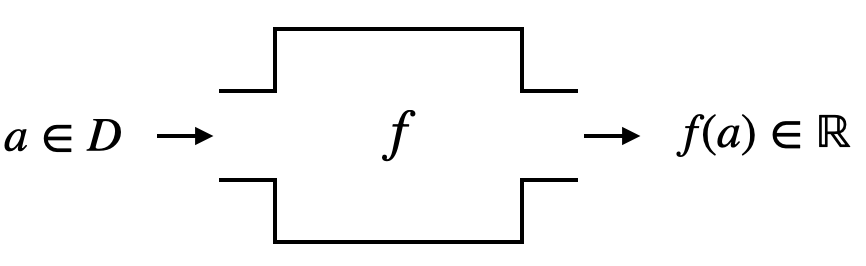
\includegraphics[width=60mm]{calculus2/function.png}
 \end{center}
\end{figure}

\vspace{-2mm}

\end{frame}



%%%%%%%%%%%%%%%%%%%%%%%%%%%%%%%%%%%%%%%%%%%%%%%%%%%%%%%%%%%%%%%%%%%%%%%%%%%%%%%%%%%%%%%
%%%%%%%%%%%%%%%%%%%%%%%%%%%%%%%%%%%%%%%%%%%%%%%%%%%%%%%%%%%%%%%%%%%%%%%%%%%%%%%%%%%%%%%

\section{関数}

\begin{frame}
\frametitle{関数}   



例えば, 関数
$$
f: \R \longrightarrow \R, \ x \mapsto (1+x)^2
$$
はしばしば単に$f(x)=(1+x)^2$と書かれる. \\
\ \\

これは$a \in D=\R$に対して$(1+a)^2 \in \R$を返す「対応」だと考えられる. 
つまり
$$
f(-1)=0, \ \ \ f(0)=1, \ \ \ f(0.3)=1.69, \ \ \ f(10)=121
$$
といった具合である. \\
\ \\

$f$の像は$\R_{\ge 0}=\{x \in \R \ | \ x \ge 0\}$である. 

\end{frame}



%%%%%%%%%%%%%%%%%%%%%%%%%%%%%%%%%%%%%%%%%%%%%%%%%%%%%%%%%%%%%%%%%%%%%%%%%%%%%%%%%%%%%%%
%%%%%%%%%%%%%%%%%%%%%%%%%%%%%%%%%%%%%%%%%%%%%%%%%%%%%%%%%%%%%%%%%%%%%%%%%%%%%%%%%%%%%%%


\begin{frame}
\frametitle{関数のグラフ}   

$xy$-平面$\R^2$上の点$(x,f(x))$を考えることで, 関数$f$を可視化できる. 
集合
$$
\{(x,f(x)) \ | \ x \in D\} \subset \R^2
$$
を関数$f$の\underline{グラフ}という. 

\begin{figure}[htbp]
 \begin{center} 
  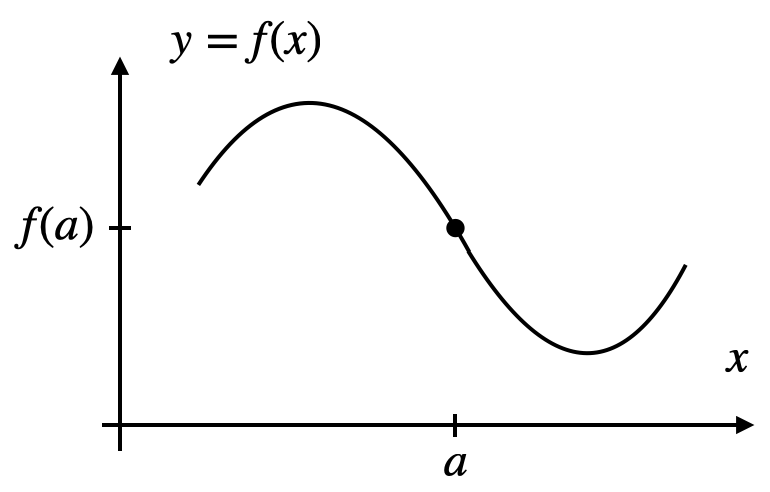
\includegraphics[width=60mm]{calculus2/graph.png}
 \end{center}
\end{figure}


\end{frame}

%%%%%%%%%%%%%%%%%%%%%%%%%%%%%%%%%%%%%%%%%%%%%%%%%%%%%%%%%%%%%%%%%%%%%%%%%%%%%%%%%%%%%%%
%%%%%%%%%%%%%%%%%%%%%%%%%%%%%%%%%%%%%%%%%%%%%%%%%%%%%%%%%%%%%%%%%%%%%%%%%%%%%%%%%%%%%%%


\begin{frame}
\frametitle{関数のグラフ}   


\begin{figure}[htbp]
 \begin{center} 
  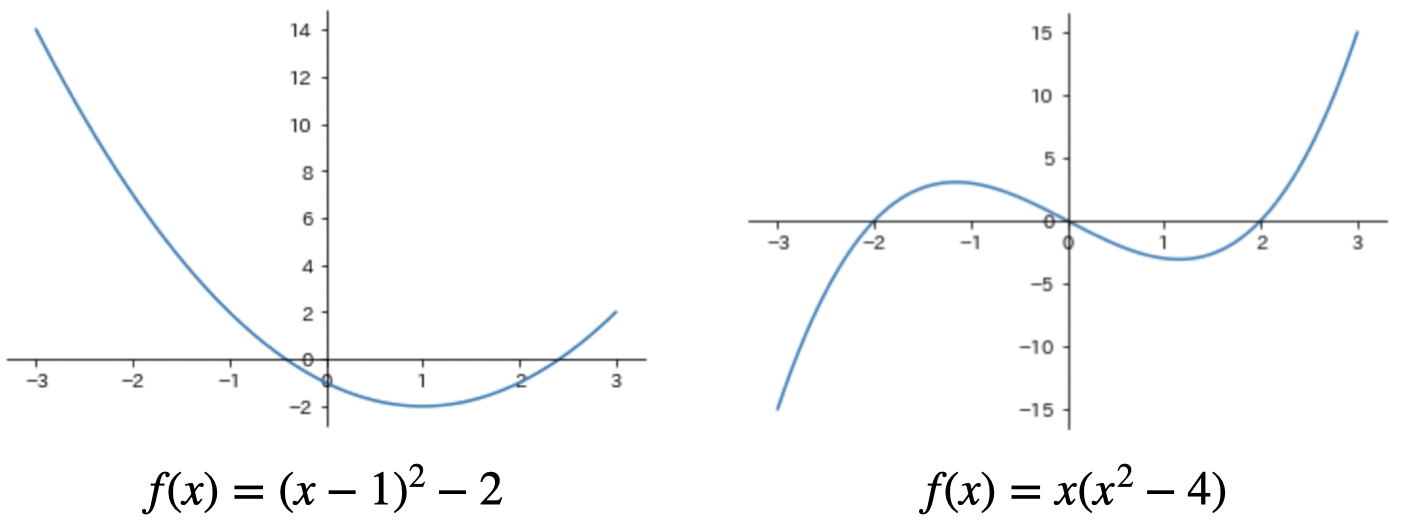
\includegraphics[width=100mm]{calculus2/graph2.png}
 \end{center}
\end{figure}


\end{frame}


%%%%%%%%%%%%%%%%%%%%%%%%%%%%%%%%%%%%%%%%%%%%%%%%%%%%%%%%%%%%%%%%%%%%%%%%%%%%%%%%%%%%%%%
%%%%%%%%%%%%%%%%%%%%%%%%%%%%%%%%%%%%%%%%%%%%%%%%%%%%%%%%%%%%%%%%%%%%%%%%%%%%%%%%%%%%%%%


\begin{frame}
\frametitle{関数のグラフ}   


\begin{Prob}
次の関数のグラフを描け. 
\begin{enumerate}
\item $f(x)=2x-5$
\item $g(x)=x^2-2x-3$
\item $h(x)=|x^2-4x-12|$
\end{enumerate}
\end{Prob}


\end{frame}





%%%%%%%%%%%%%%%%%%%%%%%%%%%%%%%%%%%%%%%%%%%%%%%%%%%%%%%%%%%%%%%%%%%%%%%%%%%%%%%%%%%%%%%
%%%%%%%%%%%%%%%%%%%%%%%%%%%%%%%%%%%%%%%%%%%%%%%%%%%%%%%%%%%%%%%%%%%%%%%%%%%%%%%%%%%%%%%


\begin{frame}
\frametitle{関数の定義域}

次の2つの関数
\begin{align*}
f_1: \{ x \in \R \ | \ x \neq 0\} \longrightarrow \R, \ x \mapsto \frac{1}{x}\\
f_2: \{ x \in \R \ | \ x > 0\} \longrightarrow \R, \ x \mapsto \frac{1}{x}
\end{align*}
は定義域が異なるので, 厳密には異なる関数である. \\
\ \\

しかしながら, 特に言及がなければ$1/x$と書かれた関数は前者を指す. 
このように, 特に定義域を指定せずに式だけで与えられた関数は, その式に代入可能な実数全体を定義域とする関数と考える.


\end{frame}


%%%%%%%%%%%%%%%%%%%%%%%%%%%%%%%%%%%%%%%%%%%%%%%%%%%%%%%%%%%%%%%%%%%%%%%%%%%%%%%%%%%%%%%
%%%%%%%%%%%%%%%%%%%%%%%%%%%%%%%%%%%%%%%%%%%%%%%%%%%%%%%%%%%%%%%%%%%%%%%%%%%%%%%%%%%%%%%


\begin{frame}
\frametitle{関数の定義域}

\begin{itemize}
\item $x^2 + 3x$は$\R$上で定義された関数. 
\item $\frac{3x+1}{x^2-5}$は分母が$0$にならない範囲, つまり$x\neq \pm \sqrt{5}$で定義された関数. 
\item $\sqrt{x-3}$は平方根の中身が非負である範囲, つまり$x\ge 3$で定義された関数. 
\end{itemize}
%定義域が$\R$である関数を\underline{全実数}という. 

\end{frame}


%%%%%%%%%%%%%%%%%%%%%%%%%%%%%%%%%%%%%%%%%%%%%%%%%%%%%%%%%%%%%%%%%%%%%%%%%%%%%%%%%%%%%%%
%%%%%%%%%%%%%%%%%%%%%%%%%%%%%%%%%%%%%%%%%%%%%%%%%%%%%%%%%%%%%%%%%%%%%%%%%%%%%%%%%%%%%%%

\section{多項式関数}


\begin{frame}
\frametitle{多項式関数}

\begin{itemize}
\item 
$a_0,a_1,\dots,a_n \in \R$に対して, 
$$
f(x)=a_nx^n+a_{n-1}x^{n-1}+\dots+a_1x+a_0
$$
の形の関数を\underline{多項式関数}という. 
\item 例
$$
-2x+3, \ \ \ x^3-x^2+7x+10, \ \ \ x^{100} 
$$
\item $a_i$は$x^i$の\underline{係数}, $a_0$は\underline{定数項}と呼ばれる. 
\item $a_n \neq 0$であるとき, $n$を$f(x)$の\underline{次数}, $f(x)$を$n$次多項式関数という. 
\item 多項式関数の定義域は$\R$. 
\end{itemize}

\end{frame}



%%%%%%%%%%%%%%%%%%%%%%%%%%%%%%%%%%%%%%%%%%%%%%%%%%%%%%%%%%%%%%%%%%%%%%%%%%%%%%%%%%%%%%%
%%%%%%%%%%%%%%%%%%%%%%%%%%%%%%%%%%%%%%%%%%%%%%%%%%%%%%%%%%%%%%%%%%%%%%%%%%%%%%%%%%%%%%%


\section{有理関数}

\begin{frame}
\frametitle{有理関数}

\begin{itemize}
\item 
多項式関数$f(x),g(x)$の有理式, つまり
$$
h(x)=\frac{f(x)}{g(x)}
$$
の形で書かれる関数を\underline{有理関数}という. 
\item 例
$$
\frac{1}{x+1}, \ \ \ \frac{1}{x}+\frac{1}{x+1}, \ \ \ \frac{(x-1)(x+5)}{(x-3)(x+1)(x-7)}
$$
\item 多項式関数は有理関数の特別な場合($g(x)=1$の場合). 
\item 有理関数の定義域は$D=\{ x \in \R \ | g(x) \neq 0\}$.
\end{itemize}
%(共通因子に関しては, 後で詳しく議論する.)

\end{frame}


%%%%%%%%%%%%%%%%%%%%%%%%%%%%%%%%%%%%%%%%%%%%%%%%%%%%%%%%%%%%%%%%%%%%%%%%%%%%%%%%%%%%%%%
%%%%%%%%%%%%%%%%%%%%%%%%%%%%%%%%%%%%%%%%%%%%%%%%%%%%%%%%%%%%%%%%%%%%%%%%%%%%%%%%%%%%%%%


\section{無理関数}

\begin{frame}
\frametitle{無理関数}

\begin{itemize}
\item 
多項式と根号の有理式で表され, 変数が根号に含まれる関数を\underline{無理関数}という. 
\item 例
$$
\sqrt{x^2-1}+x^3+\frac{5}{2}, \ \ \ \frac{\sqrt{x}}{x-1}+2, \ \ \ \sqrt[3]{\frac{x^2+x+1}{5x^2-7}}+100x
$$
\item 無理関数の定義域は一般に複雑である. 例えば, 上の関数の定義域はそれぞれ
$$
\{x \in \R \ | \ x^2 \ge 1\}, \ \ \ \{x \in \R \ | \ x \ge 0, x \neq 1\}, \ \ \ \{x \in \R \ | \ x \neq \pm \sqrt{7/5}\}
$$
\end{itemize}

\end{frame}


%%%%%%%%%%%%%%%%%%%%%%%%%%%%%%%%%%%%%%%%%%%%%%%%%%%%%%%%%%%%%%%%%%%%%%%%%%%%%%%%%%%%%%%
%%%%%%%%%%%%%%%%%%%%%%%%%%%%%%%%%%%%%%%%%%%%%%%%%%%%%%%%%%%%%%%%%%%%%%%%%%%%%%%%%%%%%%%

\section{三角関数}


\begin{frame}
\frametitle{三角関数}

\begin{itemize}
\item 
\underline{三角関数}: 平面三角法の角度と線分長の関係を記述する関数の族, 及びそれらを拡張して得られる関数の総称. 
\item 正弦関数$\sin \theta$, 余弦関数$\cos \theta$, 正接関数$\tan \theta= \sin \theta / \cos \theta$が代表的. 
\item 大学では, 変数$\theta$の単位として, 度数法(度)ではなく弧度法(radian)を考えることが多い. 
$1$ radian: ``半径=弧長"なる角度. 
\item $2\pi$ rad = $360^\circ$, つまり$1$ rad =  $360^\circ/2 \pi \approx 57.3 ^\circ$. 
\end{itemize}

\vspace{-2mm}

\begin{figure}[htbp]
 \begin{center} 
  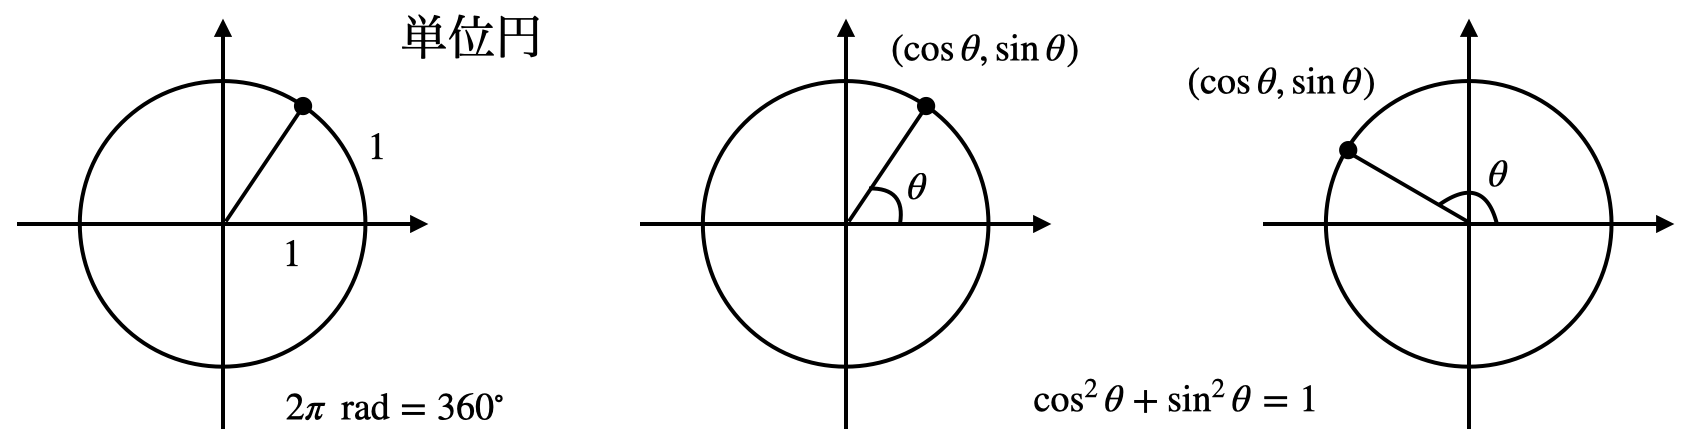
\includegraphics[width=115mm]{calculus2/radian.png}
 \end{center}
\end{figure}
\vspace{-2mm}

\end{frame}




%%%%%%%%%%%%%%%%%%%%%%%%%%%%%%%%%%%%%%%%%%%%%%%%%%%%%%%%%%%%%%%%%%%%%%%%%%%%%%%%%%%%%%%
%%%%%%%%%%%%%%%%%%%%%%%%%%%%%%%%%%%%%%%%%%%%%%%%%%%%%%%%%%%%%%%%%%%%%%%%%%%%%%%%%%%%%%%




\begin{frame}
\frametitle{三角関数}

$0 <\theta <\pi/2$であるとき

%\vspace{-2mm}
\begin{figure}[htbp]
 \begin{center} 
  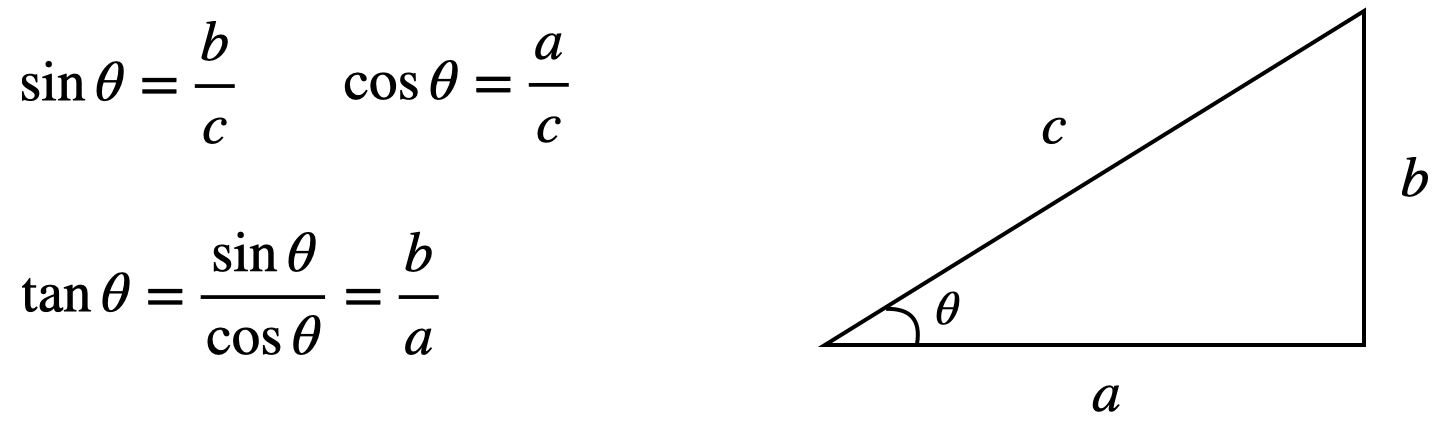
\includegraphics[width=90mm]{calculus2/sin_cos_tan.png}
 \end{center}
\end{figure}
%\vspace{-4mm}

具体的には
\begin{itemize}
\item $\sin(\pi/6)=1/2$, $\sin(\pi/4)=1/\sqrt{2}$, $\sin(\pi/3) =\sqrt{3}/2$, 
\item $\cos(\pi/6)=\sqrt{3}/2$, $\cos(\pi/4)=1/\sqrt{2}$, $\cos(\pi/3)=1/2$
\item  $\tan(\pi/6)=1/\sqrt{3}$, $\tan(\pi/4)=1$, $\tan(\pi/3)=\sqrt{3}$
\end{itemize}


\end{frame}



%%%%%%%%%%%%%%%%%%%%%%%%%%%%%%%%%%%%%%%%%%%%%%%%%%%%%%%%%%%%%%%%%%%%%%%%%%%%%%%%%%%%%%%
%%%%%%%%%%%%%%%%%%%%%%%%%%%%%%%%%%%%%%%%%%%%%%%%%%%%%%%%%%%%%%%%%%%%%%%%%%%%%%%%%%%%%%%




\begin{frame}
\frametitle{三角関数の性質}

\begin{itemize}
\item 周期: $\sin (x + 2\pi) = \sin x$, $\cos (x + 2\pi) = \cos x$, $\tan (x +\pi) = \tan x$
\item $\sin(\alpha+\beta)=\sin \alpha \cos \beta + \cos \alpha \sin \beta$
\item $\cos(\alpha+\beta)=\cos \alpha \cos \beta - \sin \alpha \sin \beta$
\end{itemize}

\vspace{-2mm}

\begin{figure}[htbp]
 \begin{center} 
  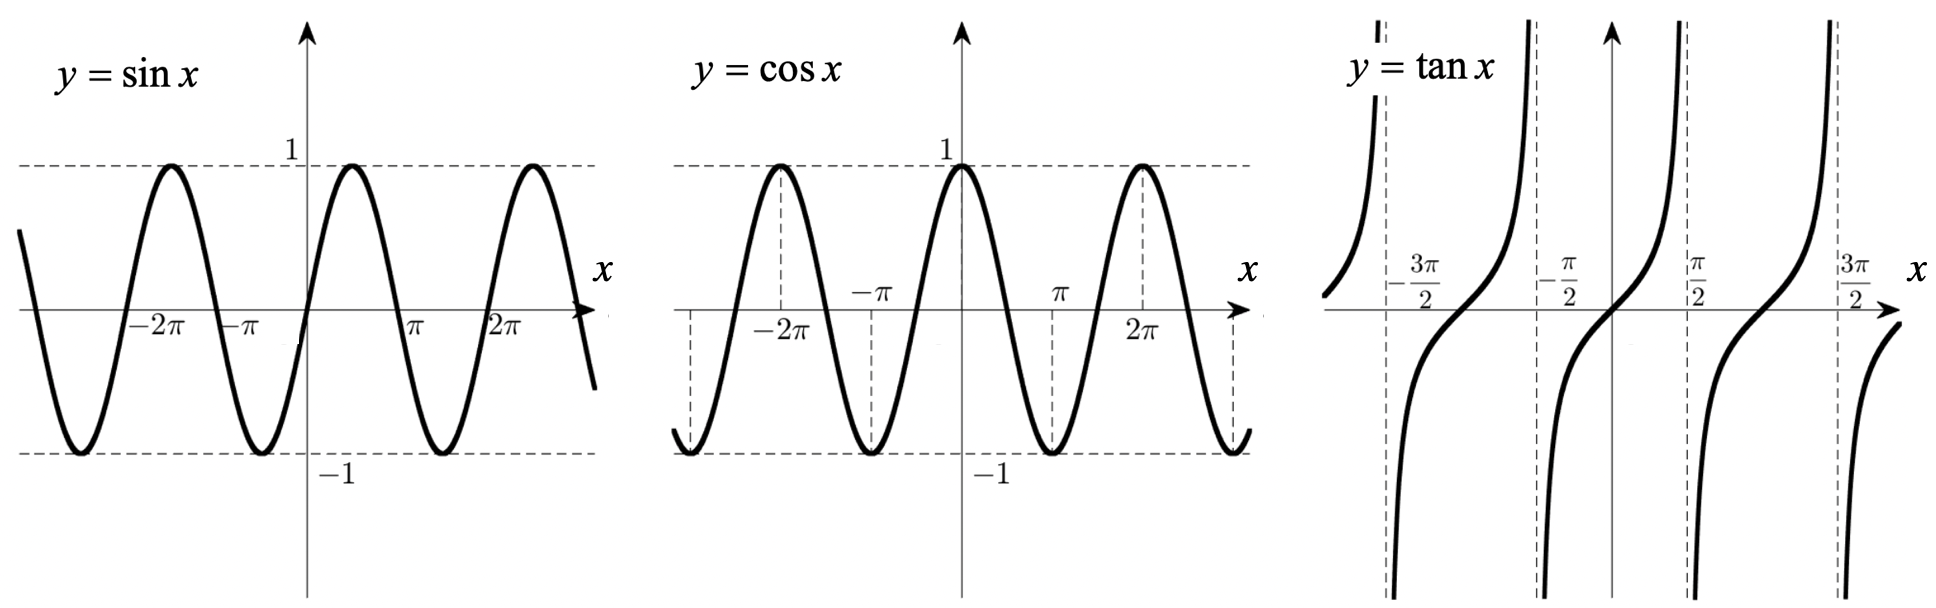
\includegraphics[width=122mm]{calculus2/trig.png}
 \end{center}
\end{figure}
\vspace{-4mm}

\end{frame}



%%%%%%%%%%%%%%%%%%%%%%%%%%%%%%%%%%%%%%%%%%%%%%%%%%%%%%%%%%%%%%%%%%%%%%%%%%%%%%%%%%%%%%%
%%%%%%%%%%%%%%%%%%%%%%%%%%%%%%%%%%%%%%%%%%%%%%%%%%%%%%%%%%%%%%%%%%%%%%%%%%%%%%%%%%%%%%%




\begin{frame}
\frametitle{三角関数の性質}

\begin{Prob}
三角関数$\sin x$, $\cos x$, $\tan x$の定義域と像を求めよ.  
\end{Prob}

\begin{Prob}
次の関数のグラフを描け. 
\begin{enumerate}
\item $3\sin(2x)$
\item $\cos(x+\frac{\pi}{3})$ + 1
\end{enumerate}
\end{Prob}

一般に, $a,b,c,d \in \R$に対して, $af(bx+c)+d$のグラフは$f(x)$のグラフを$x$軸方向に$1/b$倍し, $c$だけ左にずらし, $y$軸方向に$a$倍し, $d$だけ上にずらしたもの. 
\end{frame}


%%%%%%%%%%%%%%%%%%%%%%%%%%%%%%%%%%%%%%%%%%%%%%%%%%%%%%%%%%%%%%%%%%%%%%%%%%%%%%%%%%%%%%%
%%%%%%%%%%%%%%%%%%%%%%%%%%%%%%%%%%%%%%%%%%%%%%%%%%%%%%%%%%%%%%%%%%%%%%%%%%%%%%%%%%%%%%%

\section{指数関数}


\begin{frame}
\frametitle{指数関数}

\begin{itemize}
\item  $n\in \N$, $a >0$に対して, 冪乗$a^n =\overbrace{ a \times a \times \dots \times a}^\text{$n$個}$であった. 
$a$は\underline{底}, $n$は\underline{指数}と呼ばれる. 
さらに$a^{-n}=1/a^n$, $a^0=1$と定めることで, 指数が整数の場合にも冪乗が定義される. 
\item 例
$$
2^5=32, \ \ \ 2^{-4}=\frac{1}{16}, \ \ 2^0=1. 
$$
\item 有理数$x \in \Q$に対して, $a$の冪乗$a^x$を次のように定義する. 
$m \in \N$, $n\in \Z$, $a>0$に対して, 
$$
a^{\frac{n}{m}}=\sqrt[m]{a^n} \ (=(\sqrt[m]{a})^n). 
$$
\item 例
$$
5^{\frac{2}{3}}=\sqrt[3]{5^2} \approx 2.924,  \ \ \ 2^{-\frac{3}{4}}=2^{\frac{-3}{4}}=\sqrt[4]{1/2^3} \approx 0.5946.  
$$
\end{itemize}



\end{frame}


%%%%%%%%%%%%%%%%%%%%%%%%%%%%%%%%%%%%%%%%%%%%%%%%%%%%%%%%%%%%%%%%%%%%%%%%%%%%%%%%%%%%%%%
%%%%%%%%%%%%%%%%%%%%%%%%%%%%%%%%%%%%%%%%%%%%%%%%%%%%%%%%%%%%%%%%%%%%%%%%%%%%%%%%%%%%%%%




\begin{frame}
\frametitle{指数関数}

\begin{itemize}
\item 上の考察を元にして$x \in \R$に対して$a^x \in \R$が定義される. (厳密には有理数の稠密性を議論する必要があるが省略)
\item 関数$f(x)=a^x$を$a$を底とする\underline{指数関数}という, 
\item ネイピア数$e=2.7182\dots$を底とする場合が多い. 
\end{itemize}


\vspace{-1mm}

\begin{figure}[htbp]
 \begin{center} 
  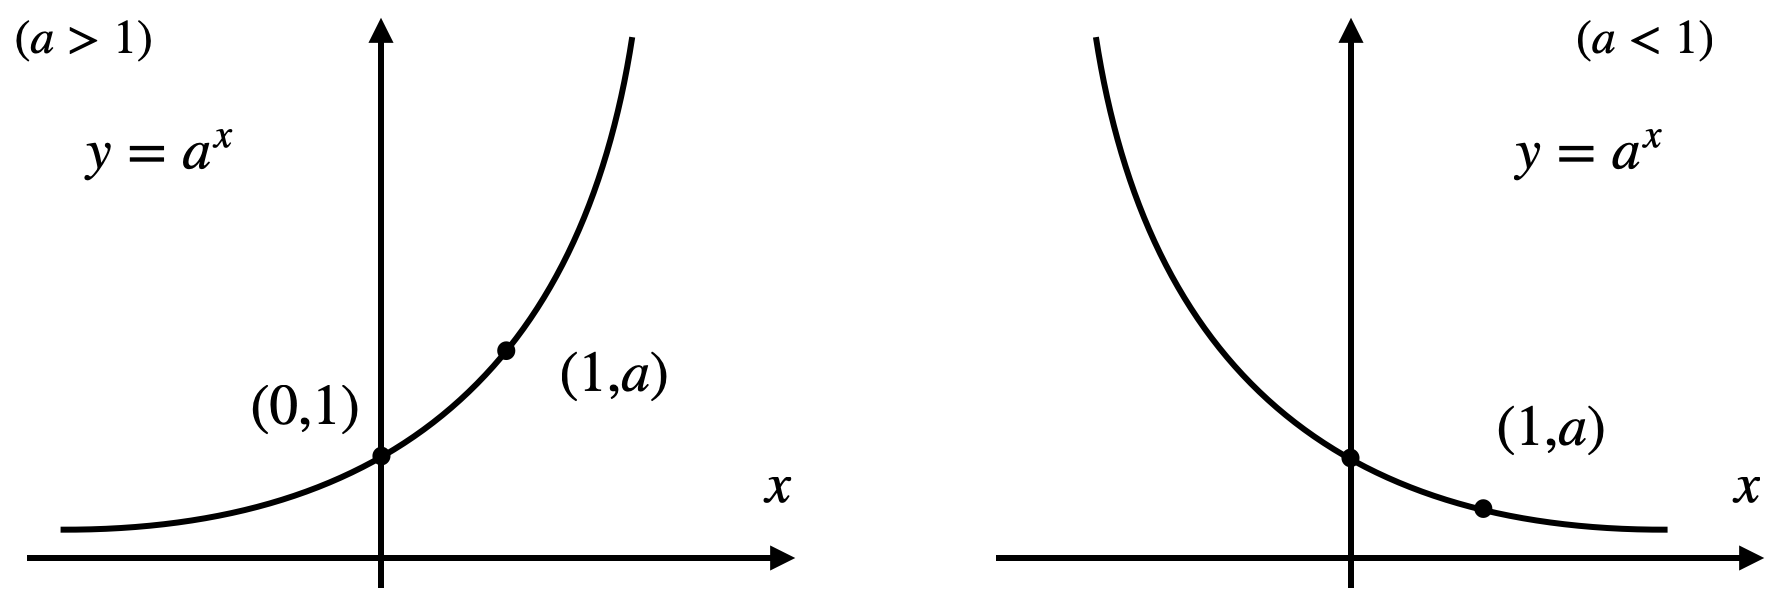
\includegraphics[width=100mm]{calculus2/exp.png}
 \end{center}
\end{figure}
\vspace{-4mm}


\end{frame}




%%%%%%%%%%%%%%%%%%%%%%%%%%%%%%%%%%%%%%%%%%%%%%%%%%%%%%%%%%%%%%%%%%%%%%%%%%%%%%%%%%%%%%%
%%%%%%%%%%%%%%%%%%%%%%%%%%%%%%%%%%%%%%%%%%%%%%%%%%%%%%%%%%%%%%%%%%%%%%%%%%%%%%%%%%%%%%%

\section{対数関数}

\begin{frame}
\frametitle{対数関数}   

\begin{itemize}
\item 
$a \ne 1$を正の実数とすると, 任意の$x \in \R_+$に対して
$$
x=a^y
$$
を満たす$y \in \R$が唯一つ存在する. これを$y=\log_a x$と書き, $a$を底とする$x$の\underline{対数}という. 
\item $f(x)=\log_a x$を$a$を底とする\underline{対数関数}という. 
定義域が$\R_+$であることに注意($f: \R_{+} \rightarrow \R, x \mapsto \log_a x$).   
\end{itemize}

例
$$
 \log_2 \frac{1}{2}=-1, \  \log_2 1=0, \ \log_2 2=1, \  \log_2 4=2, \  \log_2 8=3, \  \log_2 16=4
$$
($2^{-1}=1/2$, $2^{0}=1$, $2^{1}=2$, $2^{2}=4$, $2^{3}=8$, $2^{4}=16$)


\end{frame}



%%%%%%%%%%%%%%%%%%%%%%%%%%%%%%%%%%%%%%%%%%%%%%%%%%%%%%%%%%%%%%%%%%%%%%%%%%%%%%%%%%%%%%%
%%%%%%%%%%%%%%%%%%%%%%%%%%%%%%%%%%%%%%%%%%%%%%%%%%%%%%%%%%%%%%%%%%%%%%%%%%%%%%%%%%%%%%%


\begin{frame}
\frametitle{対数関数}   

\begin{itemize}
\item 定義より, $a^{\log_a x}=x$, $\log_a a=1$, $\log_a 1=0$. 
\item 特別な底に関して, 対数は特別な名前を持つ: 
\begin{enumerate}
\item 常用対数: $\log_{10} x=\mathrm{Log} x$, 
\item 自然対数: $\log_e x=\log x, \ln x$, 
\item 二進対数: $\log_2 x$.  
\end{enumerate}
\end{itemize}

\vspace{-1mm}

\begin{figure}[htbp]
 \begin{center} 
  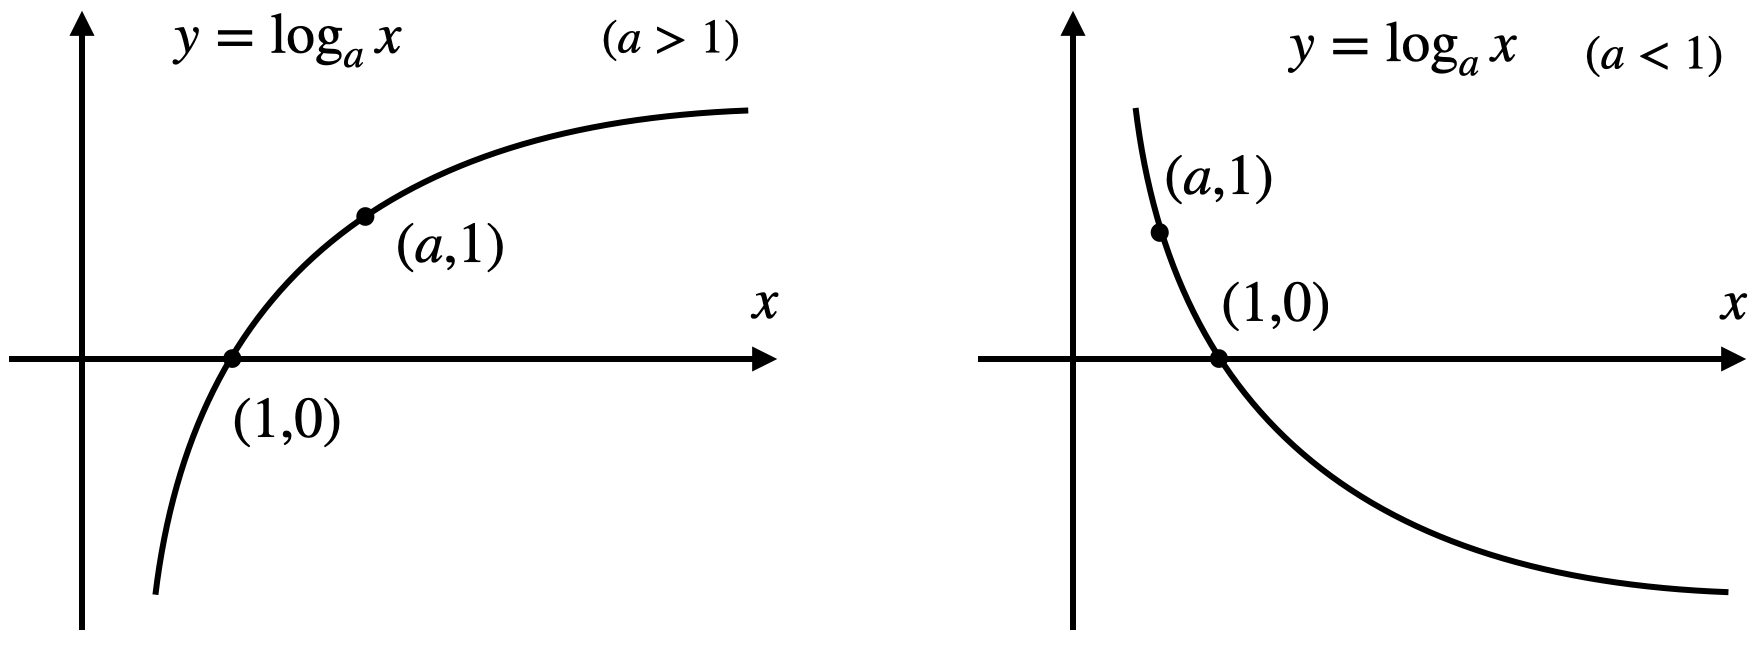
\includegraphics[width=100mm]{calculus2/log.png}
 \end{center}
\end{figure}
\vspace{-4mm}

\end{frame}



%%%%%%%%%%%%%%%%%%%%%%%%%%%%%%%%%%%%%%%%%%%%%%%%%%%%%%%%%%%%%%%%%%%%%%%%%%%%%%%%%%%%%%%
%%%%%%%%%%%%%%%%%%%%%%%%%%%%%%%%%%%%%%%%%%%%%%%%%%%%%%%%%%%%%%%%%%%%%%%%%%%%%%%%%%%%%%%


\begin{frame}
\frametitle{対数関数}   


\begin{Thm}
\begin{itemize}
\item $\log_a xy= \log_a x + \log_a y$
\item $\log_a x^b = b \log_a x$
\item (底の変換公式) 正の実数$a,b(\ne1)$と$x$に対して
$$
\log_a x = \frac{\log_b x}{\log_b a}. 
$$
\end{itemize}
\end{Thm}

例
\begin{itemize}
\item $\log_2 10 = \log_2 2+\log_2 5 =1+ \log_2 5$, 
\item $\log_3 12= \log_3 3 + \log_3 2^2=1+2 \log_3 2$, 
\item $\log_5 \frac{15}{4} = \log_5 15 +\log_5 \frac{1}{2^2} = 1+ \log_5 3 - 2\log_5 2$, 
\item $\log_7 5= \log_2 5 / \log_2 7$. 
\end{itemize}


\end{frame}



%%%%%%%%%%%%%%%%%%%%%%%%%%%%%%%%%%%%%%%%%%%%%%%%%%%%%%%%%%%%%%%%%%%%%%%%%%%%%%%%%%%%%%%
%%%%%%%%%%%%%%%%%%%%%%%%%%%%%%%%%%%%%%%%%%%%%%%%%%%%%%%%%%%%%%%%%%%%%%%%%%%%%%%%%%%%%%%

\section{指数関数と対数関数}

\begin{frame}
\frametitle{指数関数と対数関数}   

\begin{itemize}
\item $a \ne 1$に関して, 指数関数$f(x)=a^x$の像は$\R_+$, 対数関数$g(x)=\log_ax$の定義域は$\R_+$. 
\item $f(x)$と$g(x)$は互いに\underline{逆関数}(逆写像);  
$$
g(f(x))=\log_a(a^x)=x, \ \ \ f(g(x))=a^{\log_ax}=x. 
$$
\end{itemize}

\vspace{-1mm}

\begin{figure}[htbp]
 \begin{center} 
  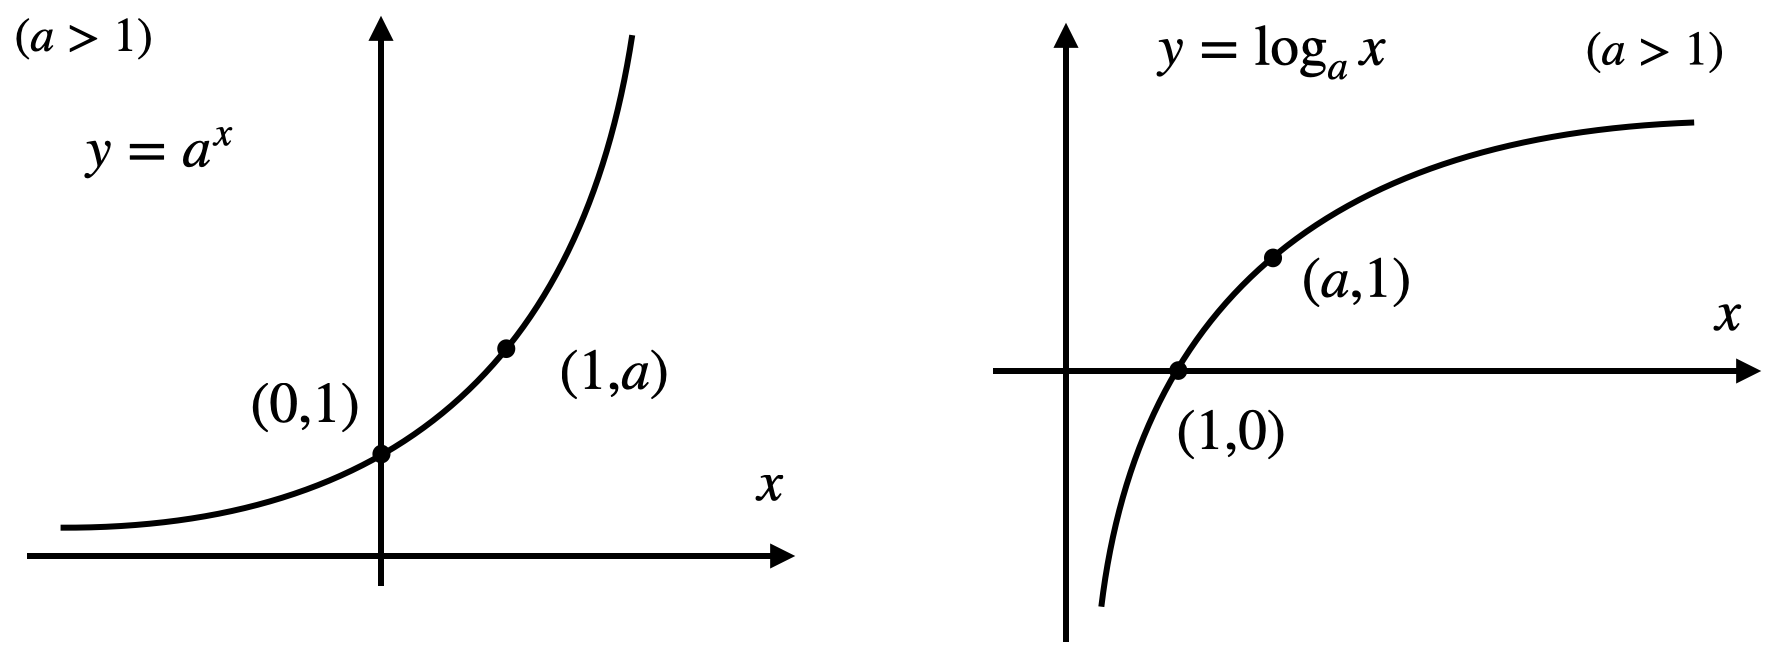
\includegraphics[width=100mm]{calculus2/exp_log.png}
 \end{center}
\end{figure}
\vspace{-4mm}

(一般に, 逆写像のグラフは$x=y$に関して鏡映対称)

\end{frame}

%%%%%%%%%%%%%%%%%%%%%%%%%%%%%%%%%%%%%%%%%%%%%%%%%%%%%%%%%%%%%%%%%%%%%%%%%%%%%%%%%%%%%%%
%%%%%%%%%%%%%%%%%%%%%%%%%%%%%%%%%%%%%%%%%%%%%%%%%%%%%%%%%%%%%%%%%%%%%%%%%%%%%%%%%%%%%%%


\section{符号関数}

\begin{frame}
\frametitle{符号関数}   

符号関数
$$
\mathrm{sgn}(x) = 
\begin{cases}
\frac{|x|}{x} & (x \ne 0) \\
0 & (x =0)
 \end{cases} \ \ 
 =
\begin{cases}
1 & (x > 0) \\
0 & (x =0) \\
-1 & (x<0)
 \end{cases}
$$

\vspace{-1mm}

\begin{figure}[htbp]
 \begin{center} 
  \includegraphics[width=45mm]{calculus2/sgn.png}
 \end{center}
\end{figure}
\vspace{-4mm}

\end{frame}



%%%%%%%%%%%%%%%%%%%%%%%%%%%%%%%%%%%%%%%%%%%%%%%%%%%%%%%%%%%%%%%%%%%%%%%%%%%%%%%%%%%%%%%
%%%%%%%%%%%%%%%%%%%%%%%%%%%%%%%%%%%%%%%%%%%%%%%%%%%%%%%%%%%%%%%%%%%%%%%%%%%%%%%%%%%%%%%




\begin{frame}
\frametitle{符号関数}   

\begin{Prob}
次の関数のグラフを描け. 
\begin{enumerate}
\item $\mathrm{sgn}(x^2)$, $\mathrm{sgn}(x^3)$
\item $\frac{x+|x|}{2x} \ \ \ (x \neq 0)$. 
\end{enumerate}
\end{Prob}
最後の関数はヘヴィサイドの階段関数と呼ばれる. 


\end{frame}




%%%%%%%%%%%%%%%%%%%%%%%%%%%%%%%%%%%%%%%%%%%%%%%%%%%%%%%%%%%%%%%%%%%%%%%%%%%%%%%%%%%%%%%
%%%%%%%%%%%%%%%%%%%%%%%%%%%%%%%%%%%%%%%%%%%%%%%%%%%%%%%%%%%%%%%%%%%%%%%%%%%%%%%%%%%%%%%

\section{床関数と天井関数}


\begin{frame}
\frametitle{床関数}   


床関数$\left \lfloor{x}\right \rfloor $
$$
\left \lfloor{x}\right \rfloor = \max\{ n \in \Z \ | \ x \ge n\}
$$
例
$$
\left \lfloor{1/2}\right \rfloor=0, \ \ \  \left \lfloor{-\pi}\right \rfloor=-4, \ \ \ \left \lfloor{5}\right \rfloor=5,  \ \ \ \left \lfloor{5.1}\right \rfloor=5
$$

\vspace{-1mm}

\begin{figure}[htbp]
 \begin{center} 
  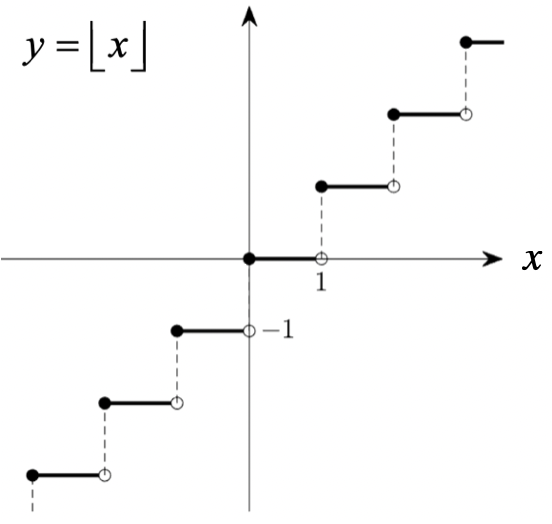
\includegraphics[width=45mm]{calculus2/floor.png}
 \end{center}
\end{figure}
\vspace{-4mm}

\end{frame}



%%%%%%%%%%%%%%%%%%%%%%%%%%%%%%%%%%%%%%%%%%%%%%%%%%%%%%%%%%%%%%%%%%%%%%%%%%%%%%%%%%%%%%%
%%%%%%%%%%%%%%%%%%%%%%%%%%%%%%%%%%%%%%%%%%%%%%%%%%%%%%%%%%%%%%%%%%%%%%%%%%%%%%%%%%%%%%%




\begin{frame}
\frametitle{天井関数}   


天井関数$\left \lceil{x}\right \rceil$
$$
\left \lceil{x}\right \rceil = \min\{ n \in \Z \ | \ x \le n\}
$$
例
$$
\left \lceil{1/2}\right \rceil =1, \ \ \  \left \lceil{-\pi}\right \rceil =-3, \ \ \ \left \lceil{5}\right \rceil =5,  \ \ \ \left \lceil{5.1}\right \rceil =6
$$

\vspace{-1mm}

\begin{figure}[htbp]
 \begin{center} 
  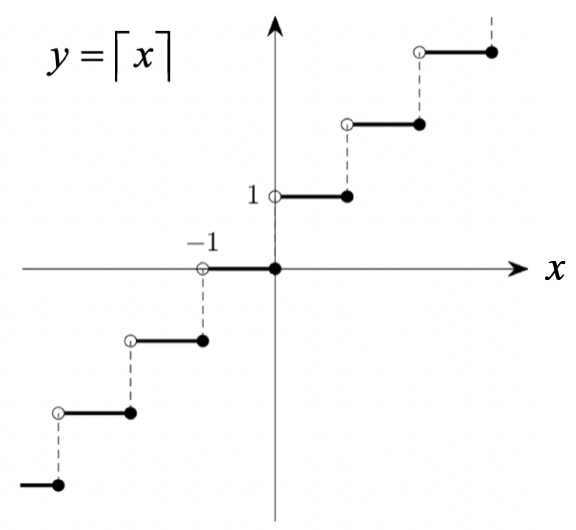
\includegraphics[width=45mm]{calculus2/ceiling.png}
 \end{center}
\end{figure}
\vspace{-4mm}

\end{frame}


%%%%%%%%%%%%%%%%%%%%%%%%%%%%%%%%%%%%%%%%%%%%%%%%%%%%%%%%%%%%%%%%%%%%%%%%%%%%%%%%%%%%%%%
%%%%%%%%%%%%%%%%%%%%%%%%%%%%%%%%%%%%%%%%%%%%%%%%%%%%%%%%%%%%%%%%%%%%%%%%%%%%%%%%%%%%%%%




\begin{frame}
\frametitle{床関数と天井関数}   


床関数$\left \lfloor{x}\right \rfloor $, 天井関数$\left \lceil{x}\right \rceil$
$$
\left \lfloor{x}\right \rfloor = \max\{ n \in \Z \ | \ x \ge n\}, \ \ \ \left \lceil{x}\right \rceil = \min\{ n \in \Z \ | \ x \le n\}
$$

\vspace{-1mm}

\begin{figure}[htbp]
 \begin{center} 
  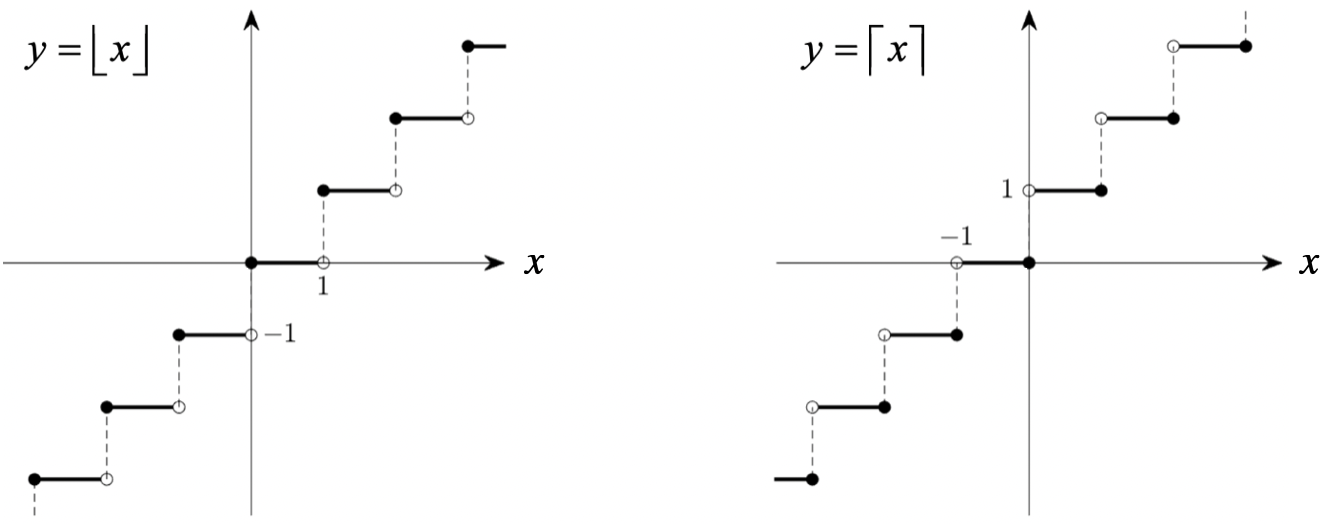
\includegraphics[width=100mm]{calculus2/floor_ceiling.png}
 \end{center}
\end{figure}
\vspace{-4mm}

\end{frame}



%%%%%%%%%%%%%%%%%%%%%%%%%%%%%%%%%%%%%%%%%%%%%%%%%%%%%%%%%%%%%%%%%%%%%%%%%%%%%%%%%%%%%%%
%%%%%%%%%%%%%%%%%%%%%%%%%%%%%%%%%%%%%%%%%%%%%%%%%%%%%%%%%%%%%%%%%%%%%%%%%%%%%%%%%%%%%%%




\begin{frame}
\frametitle{様々な関数のグラフ}   

\begin{Prob}
次の関数のグラフを描け. 
\begin{enumerate}
\item $\mathrm{sgn}(\sin x)$
\item $\left \lfloor{\frac{1}{2}x+1}\right \rfloor $
\end{enumerate}
\end{Prob}

\end{frame}



%%%%%%%%%%%%%%%%%%%%%%%%%%%%%%%%%%%%%%%%%%%%%%%%%%%%%%%%%%%%%%%%%%%%%%%%%%%%%%%%%%%%%%%
%%%%%%%%%%%%%%%%%%%%%%%%%%%%%%%%%%%%%%%%%%%%%%%%%%%%%%%%%%%%%%%%%%%%%%%%%%%%%%%%%%%%%%%




\section{今日のまとめ}
\begin{frame}
\frametitle{まとめ}   


\begin{enumerate}
\item 関数 (写像との関係, グラフ, 定義域)
\item 多項式関数, 有理関数, 無理関数, 三角関数, 指数関数, 対数関数
\item 符号関数, 床関数, 天井関数
\end{enumerate} 


\end{frame}



\section{講義概要}


\begin{frame}
\frametitle{今日の内容}



\begin{enumerate}
\item 極限 (右極限, 左極限, 極限, 極限の性質)
\item 連続 (点連続, 連続関数, 中間値の定理)
\item 不定形の極限
\end{enumerate} 



\end{frame}






%%%%%%%%%%%%%%%%%%%%%%%%%%%%%%%%%%%%%%%%%%%%%%%%%%%%%%%%%%%%%%%%%%%%%%%%%%%%%%%%%%%%%%%
%%%%%%%%%%%%%%%%%%%%%%%%%%%%%%%%%%%%%%%%%%%%%%%%%%%%%%%%%%%%%%%%%%%%%%%%%%%%%%%%%%%%%%%

\section{極限}

\begin{frame}
\frametitle{極限}



\begin{itemize}
\item 除法において, $0$で割ることは出来ない. $1/0$や$0/0$は存在しない. 
\item 無限大$\infty$と言う数は存在しない. $\infty-10$, $1/\infty$, $\infty - \infty$などは意味を持たない. 
\item しばしば, $1/0$, $1/\infty$, $\infty - \infty$などに近いものを扱う必要がある.
\begin{itemize}
\item 微分: 微小変化($0/0$に近いもの)を評価する. 
\item 積分: 微小量の無限和($\infty \times 0$に近いもの)を評価する. 
\end{itemize}
このようなものを数学的に適切に扱うために, ``極限"の概念が必要になる. 
\end{itemize}

\end{frame}





%%%%%%%%%%%%%%%%%%%%%%%%%%%%%%%%%%%%%%%%%%%%%%%%%%%%%%%%%%%%%%%%%%%%%%%%%%%%%%%%%%%%%%%
%%%%%%%%%%%%%%%%%%%%%%%%%%%%%%%%%%%%%%%%%%%%%%%%%%%%%%%%%%%%%%%%%%%%%%%%%%%%%%%%%%%%%%%


\begin{frame}
\frametitle{右極限, 左極限}

関数の値の``極限"を考えたい. 

\begin{itemize}
\item 例えば, 関数$1/x$は原点$0$では定義されないが, 原点の近傍では定義されている. 
\item $x>0$の方から原点に近付くと, 関数の値は正の値で発散, つまり$+\infty$になる. 
\item 一方で, $x<0$の方から原点に近付くと, 関数の値は負の値で発散, つまり$-\infty$になる. 
\end{itemize}

\vspace{-1mm}

 \begin{figure}[htbp]
 \begin{center} 
  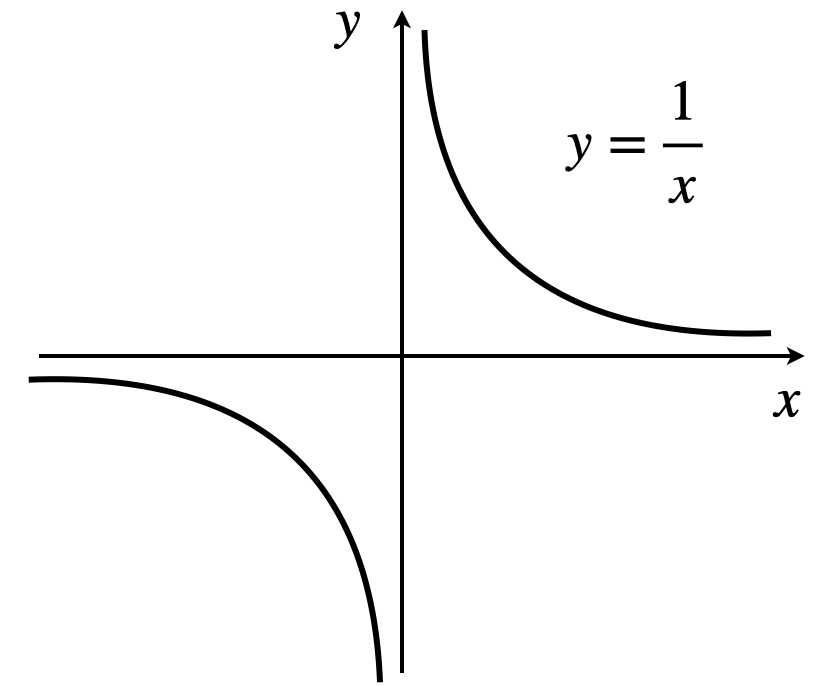
\includegraphics[width=40mm]{calculus3/xinv.png}
 \end{center}
\end{figure}

\vspace{-1mm}

\end{frame}



%%%%%%%%%%%%%%%%%%%%%%%%%%%%%%%%%%%%%%%%%%%%%%%%%%%%%%%%%%%%%%%%%%%%%%%%%%%%%%%%%%%%%%%
%%%%%%%%%%%%%%%%%%%%%%%%%%%%%%%%%%%%%%%%%%%%%%%%%%%%%%%%%%%%%%%%%%%%%%%%%%%%%%%%%%%%%%%

\section{片側極限}

\begin{frame}
\frametitle{右極限}

\begin{Def}
関数$f(x)$に関して, $x > a$を満たしながら$x$が$a$に近付くとき
\begin{itemize}
\item $f(x)$が$\alpha \in \R$に収束することを次のように表す. 
$$
\lim_{x \to a +0} f(x)=\alpha, 
$$
\item $f(x)$がいくらでも大きく(小さく)なることを, 正(負)の無限大に発散するといい,次のように表す. 
$$
\lim_{x \to a +0} f(x)=+\infty \ (-\infty)
$$
\end{itemize}
これらを$f(x)$の$a$における\underline{右極限}という. 
\end{Def}

$a=0$の場合は特別で, $x \to 0+0$と書かずに, $x\to +0$と書く. 

\end{frame}


%%%%%%%%%%%%%%%%%%%%%%%%%%%%%%%%%%%%%%%%%%%%%%%%%%%%%%%%%%%%%%%%%%%%%%%%%%%%%%%%%%%%%%%
%%%%%%%%%%%%%%%%%%%%%%%%%%%%%%%%%%%%%%%%%%%%%%%%%%%%%%%%%%%%%%%%%%%%%%%%%%%%%%%%%%%%%%%


\begin{frame}
\frametitle{左極限}

\begin{Def}
関数$f(x)$に関して, $x < a$を満たしながら$x$が$a$に近付くとき
\begin{itemize}
\item $f(x)$が$\alpha \in \R$に収束することを次のように表す. 
$$
\lim_{x \to a -0} f(x)=\alpha, 
$$
\item $f(x)$がいくらでも大きく(小さく)なることを, 正(負)の無限大に発散するといい, 次のように表す. 
$$
\lim_{x \to a -0} f(x)=+\infty \ (-\infty)
$$
\end{itemize}
これらを$f(x)$の$a$における\underline{左極限}という. 
\end{Def}

$a=0$の場合は特別で, $x \to 0-0$と書かずに, $x\to -0$と書く. 

\end{frame}

%%%%%%%%%%%%%%%%%%%%%%%%%%%%%%%%%%%%%%%%%%%%%%%%%%%%%%%%%%%%%%%%%%%%%%%%%%%%%%%%%%%%%%%
%%%%%%%%%%%%%%%%%%%%%%%%%%%%%%%%%%%%%%%%%%%%%%%%%%%%%%%%%%%%%%%%%%%%%%%%%%%%%%%%%%%%%%%


\begin{frame}
\frametitle{片側極限}

\begin{itemize}
\item 右極限と左極限は\underline{片側極限}とも呼ばれる. 
\item 関数$f(x)$の$a$における右極限と左極限は一般に一致しない. 
\item $f(a)$は定義されるとは限らないし, 定義されても極限と一致するとは限らない. 
\end{itemize}
例: $f(x)=\frac{1}{x}$, \vspace{-2mm}
$$
\lim_{x \to +0}\frac{1}{x}= +\infty, \ \ \ \lim_{x \to -0}\frac{1}{x}=-\infty
$$

\vspace{-3mm}

 \begin{figure}[htbp]
 \begin{center} 
  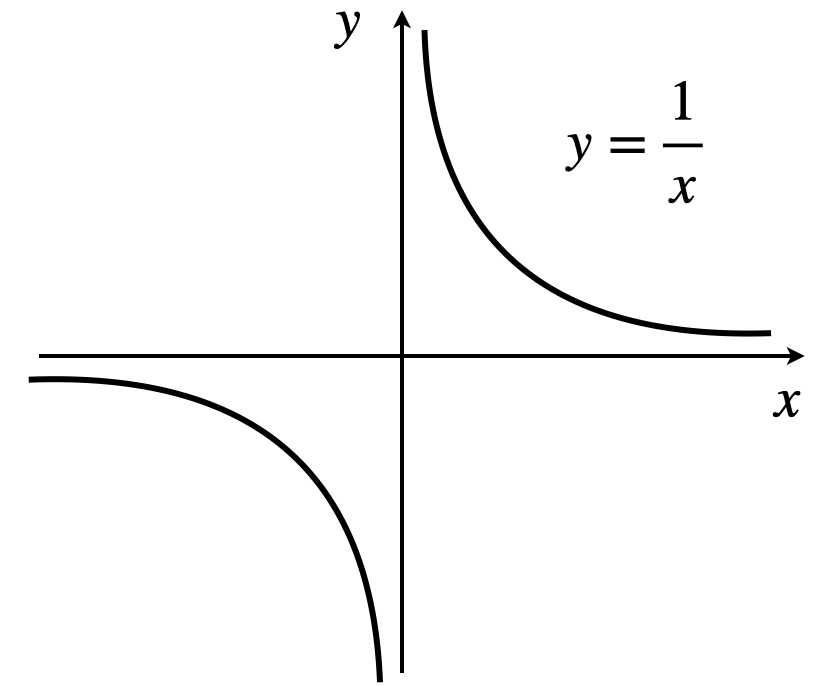
\includegraphics[width=40mm]{calculus3/xinv.png}
 \end{center}
\end{figure}

\vspace{-3mm}

\end{frame}





%%%%%%%%%%%%%%%%%%%%%%%%%%%%%%%%%%%%%%%%%%%%%%%%%%%%%%%%%%%%%%%%%%%%%%%%%%%%%%%%%%%%%%%
%%%%%%%%%%%%%%%%%%%%%%%%%%%%%%%%%%%%%%%%%%%%%%%%%%%%%%%%%%%%%%%%%%%%%%%%%%%%%%%%%%%%%%%


\begin{frame}
\frametitle{片側極限}


例: $\mathrm{sgn}(0)=0$, 
$$
\lim_{x \to +0}\mathrm{sgn}(x)=1, \ \ \ \lim_{x \to -0}\mathrm{sgn}(x)=-1
$$

\vspace{-3mm}

 \begin{figure}[htbp]
 \begin{center} 
  \includegraphics[width=45mm]{calculus3/sgn.png}
 \end{center}
\end{figure}

\vspace{-3mm}

\end{frame}




%%%%%%%%%%%%%%%%%%%%%%%%%%%%%%%%%%%%%%%%%%%%%%%%%%%%%%%%%%%%%%%%%%%%%%%%%%%%%%%%%%%%%%%
%%%%%%%%%%%%%%%%%%%%%%%%%%%%%%%%%%%%%%%%%%%%%%%%%%%%%%%%%%%%%%%%%%%%%%%%%%%%%%%%%%%%%%%

\section{極限}

\begin{frame}
\frametitle{極限} 


\begin{Def}
関数$f(x)$の$a$における右極限と左極限が存在し, それらが一致するとき, その値を
$$
\lim_{x\to a} f(x)
$$
と書いて, $f(x)$の$a$における\underline{極限}という. 
\end{Def}

つまり$x$が$a$にどのような近付き方をしても, その値が曖昧なく定まるときに極限が定義される. 
定義より, 極限が存在するとき
$$
\lim_{x\to a} f(x) = \lim_{x\to a+0} f(x) = \lim_{x\to a-0} f(x). 
$$

\end{frame}


%%%%%%%%%%%%%%%%%%%%%%%%%%%%%%%%%%%%%%%%%%%%%%%%%%%%%%%%%%%%%%%%%%%%%%%%%%%%%%%%%%%%%%%
%%%%%%%%%%%%%%%%%%%%%%%%%%%%%%%%%%%%%%%%%%%%%%%%%%%%%%%%%%%%%%%%%%%%%%%%%%%%%%%%%%%%%%%


\begin{frame}
\frametitle{極限} 


\begin{itemize}
\item 右極限と左極限が一致しないので, 極限
$$
\lim_{x\to 0}\frac{1}{x}, \ \ \ \lim_{x\to0}\mathrm{sgn}(x)
$$
は存在しない. 
\item 一方で, 
$$
\lim_{x\to +0}\frac{1}{|x|}=\lim_{x\to -0}\frac{1}{|x|}=+\infty
$$
であるから, 極限が存在して
$$
\lim_{x\to 0}\frac{1}{|x|}=\infty. 
$$
\end{itemize}

\end{frame}


%%%%%%%%%%%%%%%%%%%%%%%%%%%%%%%%%%%%%%%%%%%%%%%%%%%%%%%%%%%%%%%%%%%%%%%%%%%%%%%%%%%%%%%
%%%%%%%%%%%%%%%%%%%%%%%%%%%%%%%%%%%%%%%%%%%%%%%%%%%%%%%%%%%%%%%%%%%%%%%%%%%%%%%%%%%%%%%


\begin{frame}
\frametitle{極限} 



\begin{Prob}
\begin{itemize}
\item $\displaystyle \lim_{x\to +0}|x|$, $\displaystyle \lim_{x\to -0}|x|$を求めよ. 
\item $\displaystyle \lim_{x\to0}|x|$は存在するか? 
\end{itemize}
\end{Prob}


\begin{Prob}
\begin{itemize}
\item $\displaystyle \lim_{x\to +0}\mathrm{sgn}(|x|)$,  $\displaystyle \lim_{x\to -0}\mathrm{sgn}(|x|)$を求めよ. 
\item $\displaystyle \lim_{x\to 0}\mathrm{sgn}(|x|)$は存在するか? 
\end{itemize}
\end{Prob}

\begin{Prob}
\begin{itemize}
\item $\displaystyle \lim_{x\to +0}(x^2-x)/|x|$,   $\displaystyle \lim_{x\to -0}(x^2-x)/|x|$を求めよ. 
\item $\displaystyle \lim_{x\to 0} (x^2-x)/|x|$は存在するか? 
\end{itemize}
\end{Prob}

\end{frame}



%%%%%%%%%%%%%%%%%%%%%%%%%%%%%%%%%%%%%%%%%%%%%%%%%%%%%%%%%%%%%%%%%%%%%%%%%%%%%%%%%%%%%%%
%%%%%%%%%%%%%%%%%%%%%%%%%%%%%%%%%%%%%%%%%%%%%%%%%%%%%%%%%%%%%%%%%%%%%%%%%%%%%%%%%%%%%%%


\begin{frame}
\frametitle{注意事項} 


\begin{Rem}
\begin{itemize}
%\item ``$x$が$a$に近付くときに, $f(x)$が$\alpha$に収束する"を厳密に定義するには, $\epsilon$-$\delta$論法を用いる必要があるが, この講義では扱わない. 
\item $1/x$の例からも分かるように, $x$の近付く先$a$が定義域に含まれている必要はない. 
つまり$f(a)$が定義されていなくても, $\displaystyle \lim_{x \to a+0}f(x)$などの極限は議論できる. 
%\item 一方で, $a$が$f$の定義域$D$内の点で近似できないと$f(x)$の$a$における極限は定義できない. 
つまり, $a$は$D$もしくはその境界$\partial D$に含まれる必要がある. (閉包$\overline{D}$: $D$と$\partial D$の集合)
\end{itemize}
\end{Rem}

本講義は入門的な位置付けなので, 厳密性にはあまり拘らないで議論を進める. 

\end{frame}



%%%%%%%%%%%%%%%%%%%%%%%%%%%%%%%%%%%%%%%%%%%%%%%%%%%%%%%%%%%%%%%%%%%%%%%%%%%%%%%%%%%%%%%
%%%%%%%%%%%%%%%%%%%%%%%%%%%%%%%%%%%%%%%%%%%%%%%%%%%%%%%%%%%%%%%%%%%%%%%%%%%%%%%%%%%%%%%


\begin{frame}
\frametitle{極限の性質} 


\begin{Thm}
$\displaystyle \lim_{x\to a}f(x)=\alpha$, $\displaystyle \lim_{x\to a}g(x)=\beta$で$\alpha,\beta \in \R$とする. 
このとき
\begin{itemize}
\item $\displaystyle \lim_{x\to a} cf(x)=c \alpha$, \vspace{1mm}
\item $\displaystyle \lim_{x\to a}(f(x)+g(x))=\alpha+\beta$, \ $\displaystyle \lim_{x\to a}f(x)g(x)=\alpha\beta$,  \vspace{1mm}
\item $\beta \neq0$であれば, $\displaystyle \lim_{x\to a}f(x)/g(x)=\alpha/\beta$,  \vspace{1mm}
\item $a$の近傍で$f(x)\le g(x)$であれば, $\alpha \le \beta$, 
\end{itemize}
\end{Thm}

最後の主張は少し注意が必要で, $a$の近傍で$f(x)< g(x)$であっても$\alpha < \beta$とは限らない.  
($f(x)< g(x)$であれば$f(x)\le g(x)$なので, $\alpha \le \beta$は正しい.)

\end{frame}


%%%%%%%%%%%%%%%%%%%%%%%%%%%%%%%%%%%%%%%%%%%%%%%%%%%%%%%%%%%%%%%%%%%%%%%%%%%%%%%%%%%%%%%
%%%%%%%%%%%%%%%%%%%%%%%%%%%%%%%%%%%%%%%%%%%%%%%%%%%%%%%%%%%%%%%%%%%%%%%%%%%%%%%%%%%%%%%


%\begin{frame}
%\frametitle{極限の性質} 
%
%
%\begin{Thm}
%$\lim_{x\to a}|f(x)|=+\infty$であれば, $\lim_{x\to a}1/f(x)=0$. 
%\end{Thm}
%定理において, $a=\pm \infty$でも構わない. 
%
%
%\end{frame}



%%%%%%%%%%%%%%%%%%%%%%%%%%%%%%%%%%%%%%%%%%%%%%%%%%%%%%%%%%%%%%%%%%%%%%%%%%%%%%%%%%%%%%%
%%%%%%%%%%%%%%%%%%%%%%%%%%%%%%%%%%%%%%%%%%%%%%%%%%%%%%%%%%%%%%%%%%%%%%%%%%%%%%%%%%%%%%%


\begin{frame}
\frametitle{極限の性質} 


\begin{Prob}
次を計算せよ. 
\begin{itemize}
\item $\displaystyle \lim_{x\to 1} (x^2+3x+5)$
\item $\displaystyle \lim_{x\to 0} (2x+5)\mathrm{sgn}(|x|)$
\end{itemize}
\end{Prob}

\begin{Prob} 
$0$の近傍で$f(x)< g(x)$であり, $\displaystyle \lim_{x\to 0}f(x) = \lim_{x\to 0}g(x)$なる関数$f(x),g(x)$を1つ見つけよ.
\end{Prob}


\end{frame}




%%%%%%%%%%%%%%%%%%%%%%%%%%%%%%%%%%%%%%%%%%%%%%%%%%%%%%%%%%%%%%%%%%%%%%%%%%%%%%%%%%%%%%%
%%%%%%%%%%%%%%%%%%%%%%%%%%%%%%%%%%%%%%%%%%%%%%%%%%%%%%%%%%%%%%%%%%%%%%%%%%%%%%%%%%%%%%%


\begin{frame}
\frametitle{極限の性質} 


これまでは$a \in \R$に対して極限$\displaystyle \lim_{x \to a}f(x)$を考えていたが, $a= \pm \infty$に対しても同様の議論が可能である. 
次の定義は厳密には不十分であるが, この講義では特に問題にならない.  

\begin{itemize}
\item $x$が十分大きくなるとき, $f(x)$が$\alpha$に収束することを
$$
\lim_{x\to +\infty} f(x)=\alpha, 
$$
\item $x$が十分小さくなるとき, $f(x)$が$\alpha$に収束することを
$$
\lim_{x\to -\infty} f(x)=\alpha
$$
\end{itemize}
と書く. 

\end{frame}




%%%%%%%%%%%%%%%%%%%%%%%%%%%%%%%%%%%%%%%%%%%%%%%%%%%%%%%%%%%%%%%%%%%%%%%%%%%%%%%%%%%%%%%
%%%%%%%%%%%%%%%%%%%%%%%%%%%%%%%%%%%%%%%%%%%%%%%%%%%%%%%%%%%%%%%%%%%%%%%%%%%%%%%%%%%%%%%

\section{連続}

\begin{frame}
\frametitle{連続} 


\begin{Def}
\begin{itemize}
\item $f(x)$が\underline{$a$で連続}であるとは, 
$$
\lim_{x\to a}f(x)=f(a)
$$
が成立すること. 
つまり, 極限$\displaystyle \lim_{x\to a}f(x)$が存在し, $f(a) \in \R$が定義され, それらが一致すること. 
連続でないとき, \underline{不連続}という. 
\item $f(x)$が\underline{連続関数}であるとは, 定義域の全ての点において連続であること. 
\end{itemize}
\end{Def}

$f(x)$が$a$で連続であるとき, $\displaystyle \lim_{x\to a}f(x) \neq \pm  \infty$であることに注意. 

\end{frame}



%%%%%%%%%%%%%%%%%%%%%%%%%%%%%%%%%%%%%%%%%%%%%%%%%%%%%%%%%%%%%%%%%%%%%%%%%%%%%%%%%%%%%%%
%%%%%%%%%%%%%%%%%%%%%%%%%%%%%%%%%%%%%%%%%%%%%%%%%%%%%%%%%%%%%%%%%%%%%%%%%%%%%%%%%%%%%%%


\begin{frame}
\frametitle{不連続} 



\begin{itemize}
\item  $1/x$や$\mathrm{sgn}(x)$は$0$において不連続. ($x\neq 0$では連続である.) 
\item $1/|x|$は$1/|0|$が定義されないから, $0$において不連続. ($\displaystyle \lim_{x\to 0}1/|x|=+\infty$でもある.)
\end{itemize}


%\vspace{-1mm}

 \begin{figure}[htbp]
 \begin{center} 
  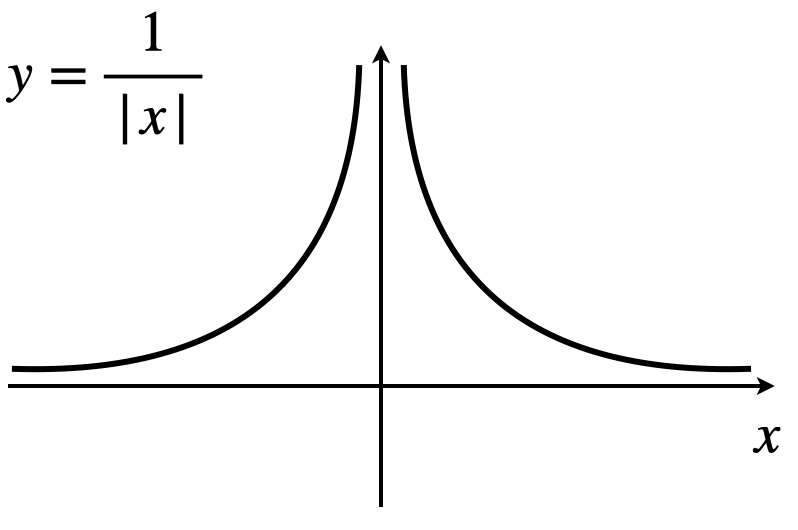
\includegraphics[width=50mm]{calculus3/xinv_abs.png}
 \end{center}
\end{figure}

\vspace{-1mm}


\end{frame}



%%%%%%%%%%%%%%%%%%%%%%%%%%%%%%%%%%%%%%%%%%%%%%%%%%%%%%%%%%%%%%%%%%%%%%%%%%%%%%%%%%%%%%%
%%%%%%%%%%%%%%%%%%%%%%%%%%%%%%%%%%%%%%%%%%%%%%%%%%%%%%%%%%%%%%%%%%%%%%%%%%%%%%%%%%%%%%%


\begin{frame}
\frametitle{不連続} 



$\mathrm{sgn}(|x|)$は, 極限$\displaystyle \lim_{x\to 0}\mathrm{sgn}(|x|)$が存在し, $\mathrm{sgn}(|0|)$も定義されるが
$$
\lim_{x\to 0}\mathrm{sgn}(|x|) \neq  \mathrm{sgn}(|0|).
$$ 

\vspace{-1mm}

 \begin{figure}[htbp]
 \begin{center} 
  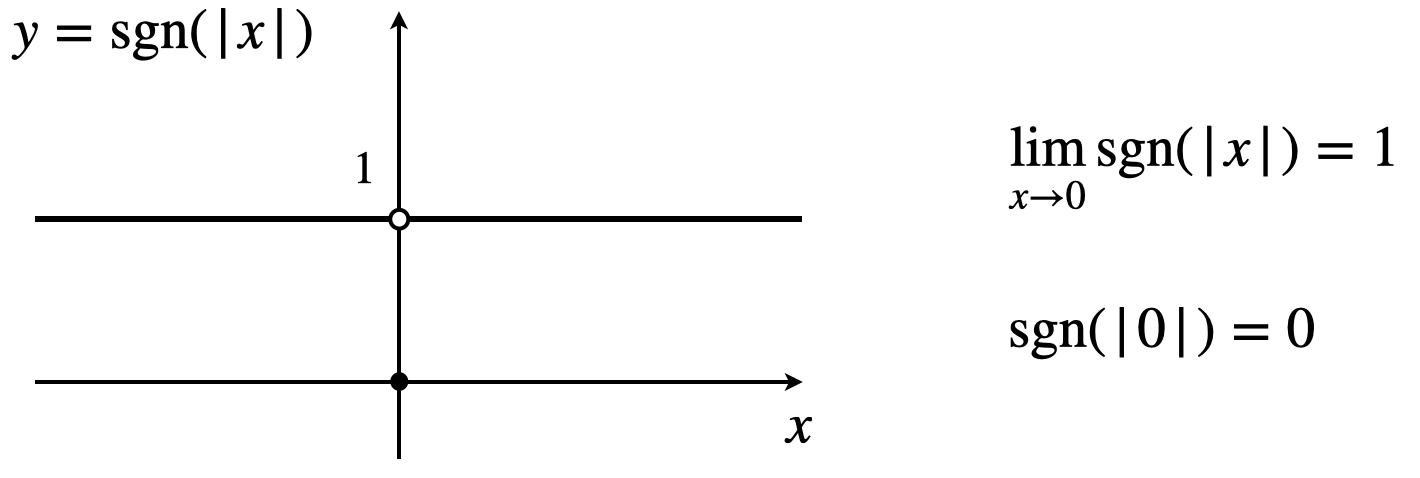
\includegraphics[width=90mm]{calculus3/sgn_abs.png}
 \end{center}
\end{figure}

\vspace{-1mm}


\end{frame}


%%%%%%%%%%%%%%%%%%%%%%%%%%%%%%%%%%%%%%%%%%%%%%%%%%%%%%%%%%%%%%%%%%%%%%%%%%%%%%%%%%%%%%%
%%%%%%%%%%%%%%%%%%%%%%%%%%%%%%%%%%%%%%%%%%%%%%%%%%%%%%%%%%%%%%%%%%%%%%%%%%%%%%%%%%%%%%%


\begin{frame}
\frametitle{連続関数の直感} 


関数$f(x)$が$a$において連続とは, $f(x)$のグラフが$(a,f(a))$で繋がっているという直感を持てば良い. 



 \begin{figure}[htbp]
 \begin{center} 
  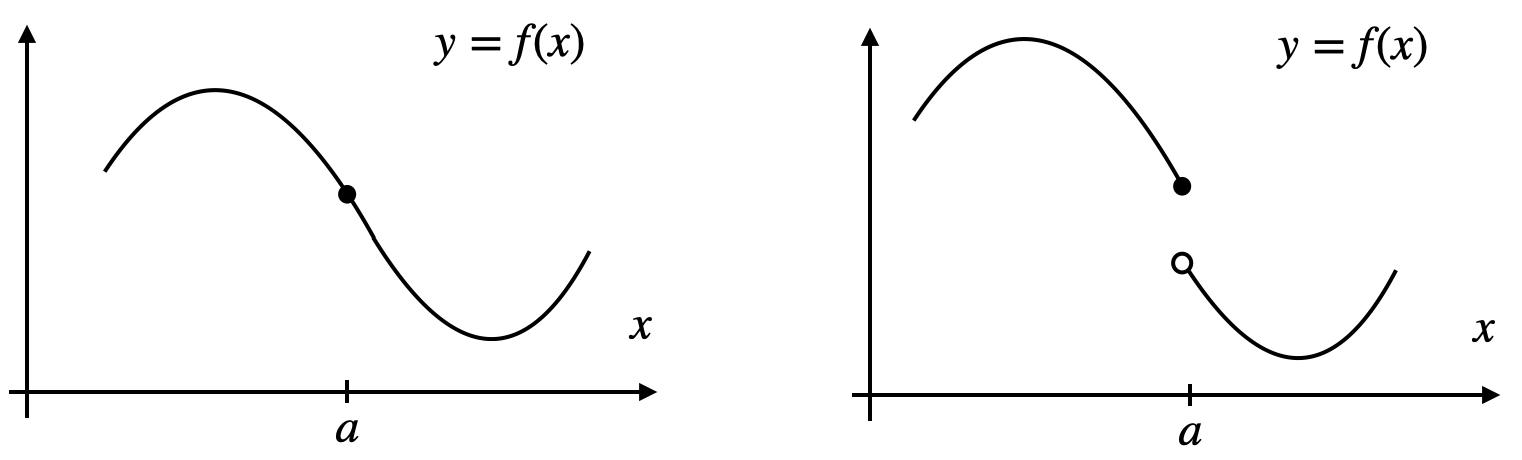
\includegraphics[width=100mm]{calculus3/(dis)conti.png}
 \end{center}
\end{figure}

左図の関数は$a$で連続, 右図の関数は$a$で不連続. 
連続関数とは, グラフが(定義域において)繋がっている, 左図のような関数. 

\end{frame}



%%%%%%%%%%%%%%%%%%%%%%%%%%%%%%%%%%%%%%%%%%%%%%%%%%%%%%%%%%%%%%%%%%%%%%%%%%%%%%%%%%%%%%%
%%%%%%%%%%%%%%%%%%%%%%%%%%%%%%%%%%%%%%%%%%%%%%%%%%%%%%%%%%%%%%%%%%%%%%%%%%%%%%%%%%%%%%%


\begin{frame}
\frametitle{連続} 



\begin{Prob}
次の関数のグラフを描け. またこれらは連続関数か? 
\begin{itemize}
\item  $|x(x+3)(x-2)|$, 
\item  $\mathrm{sgn}(\sin x)$ 
\end{itemize}
\end{Prob}


\end{frame}


%%%%%%%%%%%%%%%%%%%%%%%%%%%%%%%%%%%%%%%%%%%%%%%%%%%%%%%%%%%%%%%%%%%%%%%%%%%%%%%%%%%%%%%
%%%%%%%%%%%%%%%%%%%%%%%%%%%%%%%%%%%%%%%%%%%%%%%%%%%%%%%%%%%%%%%%%%%%%%%%%%%%%%%%%%%%%%%


\begin{frame}
\frametitle{連続関数の加減乗除} 


\begin{Thm}
$f(x )$, $g(x)$が$a$において連続であるとする. 
\begin{itemize}
\item $cf(x)$, $f(x)+g(x)$, $f(x)g(x)$は$a$において連続. 
\item $g(a) \neq0$であれば, $f(x)/g(x)$は$a$において連続. 
\end{itemize}
\end{Thm}

\begin{itemize}
\item 恒等関数$f(x)=x$が連続関数であることから, 多項式関数や有理関数も(定義域において)連続関数である.  
\item 三角関数, 指数関数, 対数関数は連続関数であることが知られているため, $2\sin x -3 \log x$や$e^x \cos x$なども連続関数. 
\end{itemize}
\end{frame}


%%%%%%%%%%%%%%%%%%%%%%%%%%%%%%%%%%%%%%%%%%%%%%%%%%%%%%%%%%%%%%%%%%%%%%%%%%%%%%%%%%%%%%%
%%%%%%%%%%%%%%%%%%%%%%%%%%%%%%%%%%%%%%%%%%%%%%%%%%%%%%%%%%%%%%%%%%%%%%%%%%%%%%%%%%%%%%%


\begin{frame}
\frametitle{合成関数の連続性} 


\begin{Thm}
関数$f(x)$, $g(x)$に関して, 関数$f(x)$の定義域は$g(a)$を含み, 関数$g(x)$は$a$において連続であり, 
関数$f(x)$は$g(a)$において連続である時, 合成関数$f(g(x))$も$a$において連続. 
\end{Thm}

例: 次の関数は連続関数
$$
\sin(x^3+5x+2), \ \ \ e^{x^3}+\log(x^2+1), \ \ \ 
$$
他にも, $\log(x+1)$は$x\le-1$で定義されないが, $x>-1$において連続. 


\end{frame}



%%%%%%%%%%%%%%%%%%%%%%%%%%%%%%%%%%%%%%%%%%%%%%%%%%%%%%%%%%%%%%%%%%%%%%%%%%%%%%%%%%%%%%%
%%%%%%%%%%%%%%%%%%%%%%%%%%%%%%%%%%%%%%%%%%%%%%%%%%%%%%%%%%%%%%%%%%%%%%%%%%%%%%%%%%%%%%%


\begin{frame}
\frametitle{中間値の定理} 

連続関数に関する最も重要な定理が, 次の中間値の定理である. 

\begin{Thm}[中間値の定理]
関数$f(x)$が閉区間$[a,b]$で連続とする. 
$f(a) \neq  f(b)$を満たすとき, 任意の$l \in [f(a), f(b)]$に対して, $l=f(c)$なる点$c \in [a,b]$が存在する. 
\end{Thm}

 \begin{figure}[htbp]
 \begin{center} 
  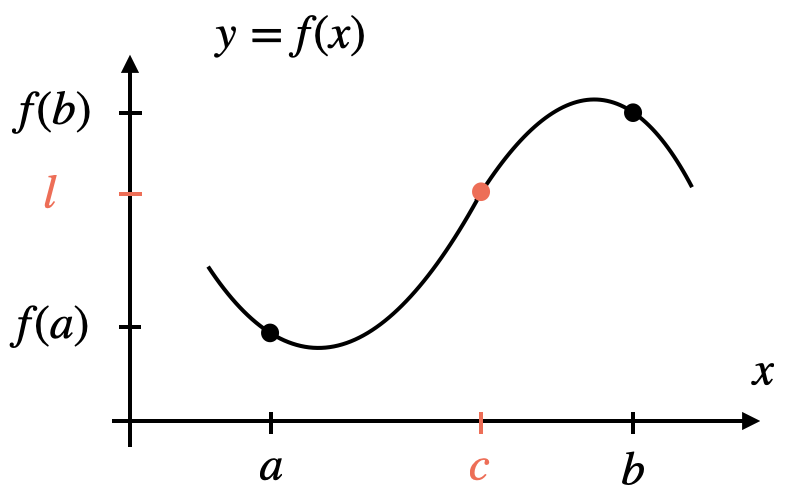
\includegraphics[width=60mm]{calculus3/mean_value.png}
 \end{center}
\end{figure}


\end{frame}

%%%%%%%%%%%%%%%%%%%%%%%%%%%%%%%%%%%%%%%%%%%%%%%%%%%%%%%%%%%%%%%%%%%%%%%%%%%%%%%%%%%%%%%
%%%%%%%%%%%%%%%%%%%%%%%%%%%%%%%%%%%%%%%%%%%%%%%%%%%%%%%%%%%%%%%%%%%%%%%%%%%%%%%%%%%%%%%


\begin{frame}
\frametitle{極限計算} 



定義より, 関数が連続な点に関しては, 極限値を単に代入することで求めることができる. \\
\ \\

例えば, $(x^2+2x-3)/(x^2-1)$は$x\neq \pm1$において連続であるから, 
$$
\lim_{x \to 3} \frac{x^2+2x-3}{x^2-1}=\frac{3^2+2\cdot 3-3}{3^2-1}=\frac{3}{2}. 
$$
一方で, $1$は$(x^2+2x-3)/(x^2-1)$の定義域に入っていないため, この点において$f(x)$は連続でない. 
無理に代入すると
$$
\lim_{x \to 1} \frac{x^2+2x-3}{x^2-1}=\frac{1^2+2\cdot 1-3}{1^2-1}=\frac{0}{0} \ \ ?? 
$$
\end{frame}



%%%%%%%%%%%%%%%%%%%%%%%%%%%%%%%%%%%%%%%%%%%%%%%%%%%%%%%%%%%%%%%%%%%%%%%%%%%%%%%%%%%%%%%
%%%%%%%%%%%%%%%%%%%%%%%%%%%%%%%%%%%%%%%%%%%%%%%%%%%%%%%%%%%%%%%%%%%%%%%%%%%%%%%%%%%%%%%


\begin{frame}
\frametitle{極限計算} 



一方で, $1$は$(x^2+2x-3)/(x^2-1)$の定義域に入っていなくても, 
\begin{align*}
\lim_{x \to 1} \frac{x^2+2x-3}{x^2-1} &= \lim_{x \to 1} \frac{(x-1)(x+3)}{(x-1)(x+1)} \\
& = \lim_{x \to 1} \frac{x+3}{x+1} \\
& =  \frac{1+3}{1+1} =2 
\end{align*}

\begin{itemize}
\item 2つ目の等号: $x \to 1$において$x-1\neq 0$であるから, 分母分子を$x-1$で割ることができる. 
\item 3つ目の等号: 連続関数なので代入して極限を求めることが可能. 
\end{itemize}


\end{frame}



%%%%%%%%%%%%%%%%%%%%%%%%%%%%%%%%%%%%%%%%%%%%%%%%%%%%%%%%%%%%%%%%%%%%%%%%%%%%%%%%%%%%%%%
%%%%%%%%%%%%%%%%%%%%%%%%%%%%%%%%%%%%%%%%%%%%%%%%%%%%%%%%%%%%%%%%%%%%%%%%%%%%%%%%%%%%%%%


\begin{frame}
\frametitle{不定形} 

一般に, $\frac{0}{0}$, $\frac{\infty}{\infty}$, $\infty - \infty$といった形は\underline{不定形}と呼ばれる. 
特別な場合にはこれらは数学的に意味を持ち, 具体的に計算可能. 
次のような例がある. 

\begin{itemize}
\item $\displaystyle \lim_{x\to 2} \frac{x^2-x-2}{x^3-8}$
%\item $\displaystyle \lim_{x\to 3} \frac{x^3+x^2-14x+6}{x^2-9}$
\item $\displaystyle \lim_{x\to 0} \frac{1}{x}(1+\frac{1}{x-1})$
\item $\displaystyle \lim_{x \to \infty}\frac{4x^3-2x^2-10}{7x^3+5x+2}$
\item $\displaystyle \lim_{x\to -\infty} (3x^3+2x^2)$
\item $\displaystyle \lim_{x\to \infty} (\sqrt{x+100}-\sqrt{x})$
\end{itemize}


\end{frame}


%%%%%%%%%%%%%%%%%%%%%%%%%%%%%%%%%%%%%%%%%%%%%%%%%%%%%%%%%%%%%%%%%%%%%%%%%%%%%%%%%%%%%%%
%%%%%%%%%%%%%%%%%%%%%%%%%%%%%%%%%%%%%%%%%%%%%%%%%%%%%%%%%%%%%%%%%%%%%%%%%%%%%%%%%%%%%%%


\begin{frame}
\frametitle{不定形} 


\begin{align*}
\lim_{x\to 2} \frac{x^2-x-2}{x^3-8}
& =  \lim_{x\to 2} \frac{(x-2)(x+1)}{(x-2)(x^2+2x+4)} \\
& =   \lim_{x\to 2}\frac{x+1}{x^2+2x+4} \\
& = \frac{3}{12}=\frac{1}{4} \\
\ & \ \\
\lim_{x\to 0} \frac{1}{x}(1+\frac{1}{x-1})
& =  \lim_{x\to 0} \frac{1}{x} \frac{x}{x-1} \\
& =  \lim_{x\to 0}\frac{1}{x-1} \\
& = -1
\end{align*}


%\begin{align*}
%\lim_{x\to 3} \frac{x^3+x^2-14x+6}{x^2-9}
%& =  \lim_{x\to 3} \frac{(x-3)(x^2+4x-2)}{(x+3)(x-3)} \\
% & =  \lim_{x\to 3} \frac{x^2+4x-2}{x+3} \\
% & = \frac{19}{6}. 
%\end{align*}


\end{frame}


%%%%%%%%%%%%%%%%%%%%%%%%%%%%%%%%%%%%%%%%%%%%%%%%%%%%%%%%%%%%%%%%%%%%%%%%%%%%%%%%%%%%%%%
%%%%%%%%%%%%%%%%%%%%%%%%%%%%%%%%%%%%%%%%%%%%%%%%%%%%%%%%%%%%%%%%%%%%%%%%%%%%%%%%%%%%%%%


\begin{frame}
\frametitle{不定形} 


\begin{align*}
\lim_{x \to \infty}\frac{4x^3-2x^2-10}{7x^3+5x+2} 
& = \lim_{x \to \infty} \frac{4-\frac{2}{x}-\frac{10}{x^3}}{7+\frac{5}{x^2}+\frac{2}{x^3}} = \frac{4}{7}. \\
\ & \ \\
\lim_{x\to -\infty} (3x^3+2x^2)
& =  \lim_{x\to -\infty} x^3(3+\frac{2}{x})  = -\infty
\end{align*}


\end{frame}


%%%%%%%%%%%%%%%%%%%%%%%%%%%%%%%%%%%%%%%%%%%%%%%%%%%%%%%%%%%%%%%%%%%%%%%%%%%%%%%%%%%%%%%
%%%%%%%%%%%%%%%%%%%%%%%%%%%%%%%%%%%%%%%%%%%%%%%%%%%%%%%%%%%%%%%%%%%%%%%%%%%%%%%%%%%%%%%


\begin{frame}
\frametitle{不定形} 


\begin{align*}
\lim_{x\to \infty} (\sqrt{x+100}-\sqrt{x})
& =  \lim_{x\to \infty} \frac{(\sqrt{x+100}-\sqrt{x})(\sqrt{x+100}+\sqrt{x})}{\sqrt{x+100}+\sqrt{x}} \\
& =  \lim_{x\to \infty} \frac{100}{ \sqrt{x+100}+\sqrt{x}} \\
& =0
\end{align*}


\end{frame}






%%%%%%%%%%%%%%%%%%%%%%%%%%%%%%%%%%%%%%%%%%%%%%%%%%%%%%%%%%%%%%%%%%%%%%%%%%%%%%%%%%%%%%%
%%%%%%%%%%%%%%%%%%%%%%%%%%%%%%%%%%%%%%%%%%%%%%%%%%%%%%%%%%%%%%%%%%%%%%%%%%%%%%%%%%%%%%%




\section{今日のまとめ}
\begin{frame}
\frametitle{まとめ}   


\begin{enumerate}
\item 極限 (右極限, 左極限, 極限, 極限の性質)
\item 連続 (点連続, 連続関数, 中間値の定理)
\item 不定形の極限
\end{enumerate} 


\end{frame}

\section{講義概要}


\begin{frame}
\frametitle{今日の内容}



\begin{enumerate}
\item 平均変化率, 微分係数, 接線の傾き
\item 導関数, 導関数の性質
\end{enumerate} 



\end{frame}





%%%%%%%%%%%%%%%%%%%%%%%%%%%%%%%%%%%%%%%%%%%%%%%%%%%%%%%%%%%%%%%%%%%%%%%%%%%%%%%%%%%%%%%
%%%%%%%%%%%%%%%%%%%%%%%%%%%%%%%%%%%%%%%%%%%%%%%%%%%%%%%%%%%%%%%%%%%%%%%%%%%%%%%%%%%%%%%

\section{極限の別表記}


\begin{frame}
\frametitle{極限の別表示}


前回, 関数$f(x)$の$a$における極限を,
$$
\lim_{x \to a +0}f(x)=\lim_{x \to a -0}f(x)=\alpha
$$
であるときに, $\displaystyle \lim_{x \to a}f(x)=\alpha$と定義した. \\
\ \\

上記の条件は, $x=a+h$と表すと, 
$$
\lim_{h \to +0}f(a+h)=\lim_{h\to -0}f(a+h)=\alpha
$$
と同値であり, これを$\displaystyle \lim_{h \to 0}f(a+h)=\alpha$と書く. 
今回の講義では後者の表記を用いる. 


\end{frame}



%%%%%%%%%%%%%%%%%%%%%%%%%%%%%%%%%%%%%%%%%%%%%%%%%%%%%%%%%%%%%%%%%%%%%%%%%%%%%%%%%%%%%%%
%%%%%%%%%%%%%%%%%%%%%%%%%%%%%%%%%%%%%%%%%%%%%%%%%%%%%%%%%%%%%%%%%%%%%%%%%%%%%%%%%%%%%%%

\section{平均変化率}

\begin{frame}
\frametitle{平均変化率}

\vspace{-5mm}

 \begin{figure}[htbp]
 \begin{center} 
  
\includegraphics[width=75mm]{calculus4/600km.png}
 \end{center}
\end{figure}

\vspace{-5mm}

\begin{Prob}
$600$kmの移動に$3$時間かかったとき, 速度は何km/hだろうか?
\end{Prob}

答えは簡単で, 
$$
\frac{\text{$600$km}}{\text{$3$時間}}=200\text{km/h}
$$
と答えたくなる. \\
\ \\

しかしながら, これは平均速度であり, 常に一定の速度で移動するとは限らない. 
つまり, ある特定の時刻での速度は必ずしも$200$km/hになるとは限らない. \\
\ \\

この問題設定からは, 平均速度しか求めることができない. 

\end{frame}





%%%%%%%%%%%%%%%%%%%%%%%%%%%%%%%%%%%%%%%%%%%%%%%%%%%%%%%%%%%%%%%%%%%%%%%%%%%%%%%%%%%%%%%
%%%%%%%%%%%%%%%%%%%%%%%%%%%%%%%%%%%%%%%%%%%%%%%%%%%%%%%%%%%%%%%%%%%%%%%%%%%%%%%%%%%%%%%


\begin{frame}
\frametitle{平均変化率}

出発からちょうど$1$時間後の速度はどのように求めれば良いだろうか? 

\vspace{-2mm}

 \begin{figure}[htbp]
 \begin{center} 
  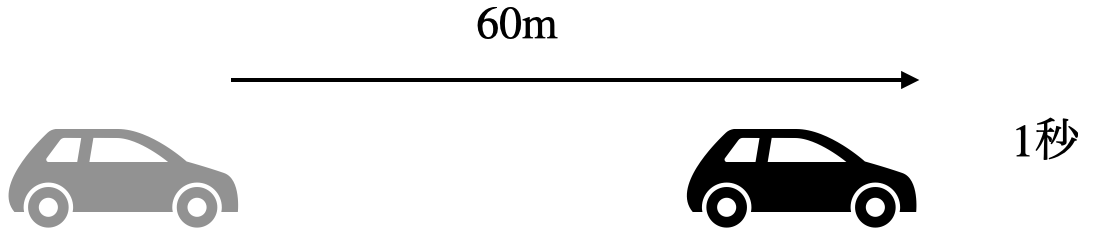
\includegraphics[width=55mm]{calculus4/60m.png}
 \end{center}
\end{figure}

\vspace{-2mm}

出発してから$1$時間後において, $1$秒間で$60$m移動したとすると, 
$$
\frac{\text{$60$m}}{\text{$1$秒}}=
\frac{\text{$0.06$km}}{\text{$1/3600$時間}}=216\text{km/h}
$$
と答えたくなる. \\
\ \\

しかしながら, 時間スケールを変えただけで, 状況は先の問題と変わっていない. 
これは$1$秒間の平均速度であり, 
$1$秒間の間に速度が変化している可能性がある. 


\end{frame}




%%%%%%%%%%%%%%%%%%%%%%%%%%%%%%%%%%%%%%%%%%%%%%%%%%%%%%%%%%%%%%%%%%%%%%%%%%%%%%%%%%%%%%%
%%%%%%%%%%%%%%%%%%%%%%%%%%%%%%%%%%%%%%%%%%%%%%%%%%%%%%%%%%%%%%%%%%%%%%%%%%%%%%%%%%%%%%%


\begin{frame}
\frametitle{平均変化率}

\vspace{-10mm}

 \begin{figure}[htbp]
 \begin{center} 
  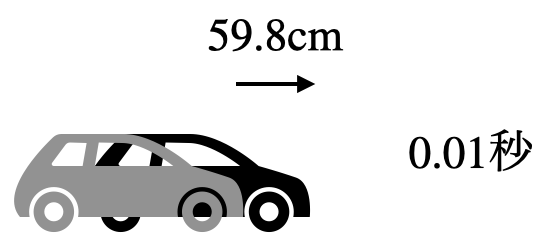
\includegraphics[width=30mm]{calculus4/59cm.png}
 \end{center}
\end{figure}

\vspace{-2mm}

時間をさらに細かく刻んで$0.01$秒間にどれだけ移動したかを計測したところ, $59.8$cm移動したことが判明した. 
するとこの$0.01$秒間の平均速度は
$$
\frac{\text{$59.8$cm}}{\text{$0.01$秒}}=
\frac{\text{$0.000598$km}}{\text{$1/360000$時間}}=215.28\text{km/h}
$$
となる. \\
\ \\

もちろんこの$0.01$秒間の間に速度が変化している可能性があるが, 良い近似になっていることが期待される.  


\end{frame}



%%%%%%%%%%%%%%%%%%%%%%%%%%%%%%%%%%%%%%%%%%%%%%%%%%%%%%%%%%%%%%%%%%%%%%%%%%%%%%%%%%%%%%%
%%%%%%%%%%%%%%%%%%%%%%%%%%%%%%%%%%%%%%%%%%%%%%%%%%%%%%%%%%%%%%%%%%%%%%%%%%%%%%%%%%%%%%%


\begin{frame}
\frametitle{平均変化率}


一般に, 時間軸をどんどん短くすることで, その時刻での速度をより正確に測定できることが期待される.\\
\ \\

つまり, ある時刻での速度は
$$
\frac{\text{微小な位置の変化}}{\text{微小な時間の変化}}
$$
の極限として得られると考えられる. \\
%ここで微小な時間の変化とは, さらに分割できないほど短い時間スケールのことである.  \\
\ \\

このような極限を扱う理論が微分である. 


\end{frame}


%%%%%%%%%%%%%%%%%%%%%%%%%%%%%%%%%%%%%%%%%%%%%%%%%%%%%%%%%%%%%%%%%%%%%%%%%%%%%%%%%%%%%%%
%%%%%%%%%%%%%%%%%%%%%%%%%%%%%%%%%%%%%%%%%%%%%%%%%%%%%%%%%%%%%%%%%%%%%%%%%%%%%%%%%%%%%%%

\section{微分係数}

\begin{frame}
\frametitle{微分係数}

\begin{Def}
関数$f(x)$の定義域を$D$とする. 
点$a \in D$に関して, 極限
$$
\lim_{h\to 0} \frac{f(a+h)-f(a)}{h}
$$
が存在するとき, $f(x)$は$a$で\underline{微分可能}であるといい, $f'(a)$で表す. 
$f'(a)$は$f(x)$の$a$における\underline{微分係数}と呼ばれる. 
\end{Def}

$f(x)$は$a$で微分可能ならば, $f(x)$は$a$で連続\footnote{$\lim_{x\to a} f(x) = f(a) \quad f(a) \in \mathbb{R}$}であることがわかるが, その逆は一般には成立しない. 



\end{frame}


%%%%%%%%%%%%%%%%%%%%%%%%%%%%%%%%%%%%%%%%%%%%%%%%%%%%%%%%%%%%%%%%%%%%%%%%%%%%%%%%%%%%%%%
%%%%%%%%%%%%%%%%%%%%%%%%%%%%%%%%%%%%%%%%%%%%%%%%%%%%%%%%%%%%%%%%%%%%%%%%%%%%%%%%%%%%%%%


\begin{frame}
\frametitle{微分係数と接線の傾き}

微分係数
$$
f'(a)=
\lim_{h\to 0} \frac{f(a+h)-f(a)}{h}
$$
は$f(x)$のグラフの点$(a,f(a))$における接線の傾きとみなすことができる. 
 

 \begin{figure}[htbp]
 \begin{center} 
  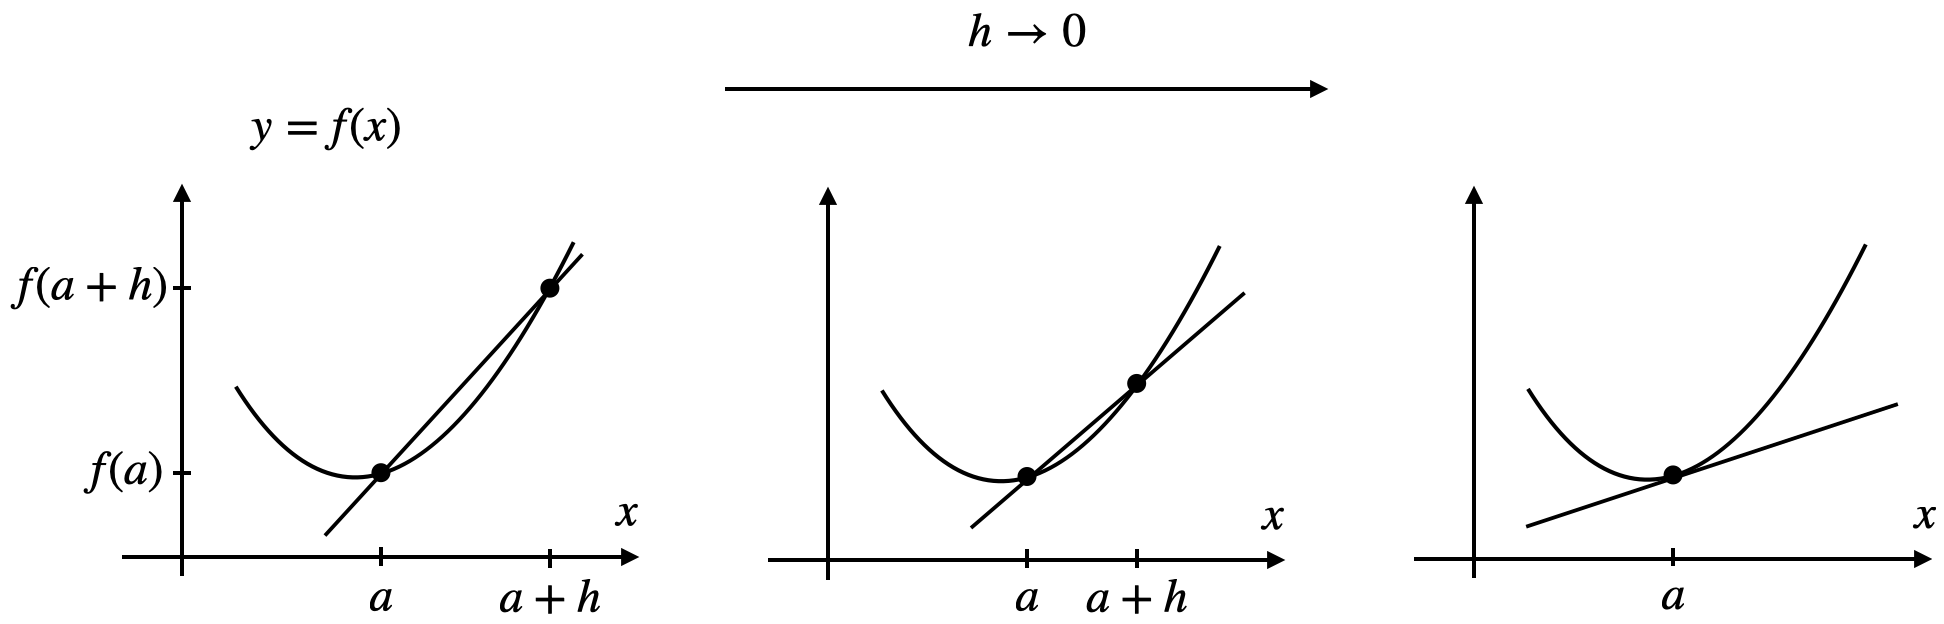
\includegraphics[width=120mm]{calculus4/tangent.png}
 \end{center}
\end{figure}


\end{frame}

%%%%%%%%%%%%%%%%%%%%%%%%%%%%%%%%%%%%%%%%%%%%%%%%%%%%%%%%%%%%%%%%%%%%%%%%%%%%%%%%%%%%%%%
%%%%%%%%%%%%%%%%%%%%%%%%%%%%%%%%%%%%%%%%%%%%%%%%%%%%%%%%%%%%%%%%%%%%%%%%%%%%%%%%%%%%%%%

\begin{frame}
\frametitle{微分可能性}

関数$f(x)$が$a$において微分可能であるとは, $f(x)$のグラフが点$(a,f(a))$における接線が定義できるくらい滑らかであることを意味する. 
点$(a,f(a))$の近傍でグラフが直線のように見えるともいえる.  
%この直線の傾きが$f'(a)$である. 


 \begin{figure}[htbp]
 \begin{center} 
  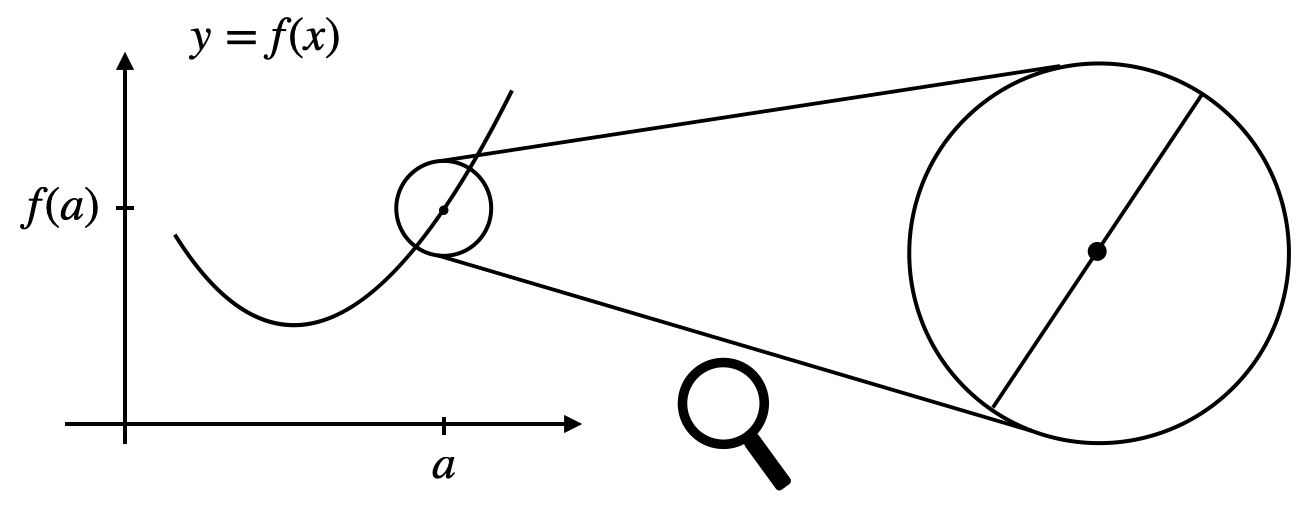
\includegraphics[width=85mm]{calculus4/differentiable2.png}
 \end{center}
\end{figure}

\end{frame}



%%%%%%%%%%%%%%%%%%%%%%%%%%%%%%%%%%%%%%%%%%%%%%%%%%%%%%%%%%%%%%%%%%%%%%%%%%%%%%%%%%%%%%%
%%%%%%%%%%%%%%%%%%%%%%%%%%%%%%%%%%%%%%%%%%%%%%%%%%%%%%%%%%%%%%%%%%%%%%%%%%%%%%%%%%%%%%

\section{導関数}

\begin{frame}
\frametitle{導関数}


\begin{Def}
関数$f(x)$がその定義域$D$の任意の点において微分可能であるとする. 
$a \in D$に対して, その点における微分係数$f'(a)$を返す関数
$$
f':D \longrightarrow \R, \ \ \ a \to f'(a)
$$
を$f(x)$の\underline{導関数}と呼び, $f'(x)$を求める事を$f(x)$を\underline{微分する}という.  
$f'(x)$は$\frac{df}{dx}(x)$と書かれる場合もある. 
\end{Def}

\end{frame}



%%%%%%%%%%%%%%%%%%%%%%%%%%%%%%%%%%%%%%%%%%%%%%%%%%%%%%%%%%%%%%%%%%%%%%%%%%%%%%%%%%%%%%%
%%%%%%%%%%%%%%%%%%%%%%%%%%%%%%%%%%%%%%%%%%%%%%%%%%%%%%%%%%%%%%%%%%%%%%%%%%%%%%%%%%%%%%

\begin{frame}
\frametitle{$(x)'=1$}


$f(x)=x$の導関数を定義に従って計算する. 
\begin{align*}
f'(x) & = \lim_{h\to 0} \frac{(x+h)-x}{h} \\
& =  \lim_{h\to 0} \frac{h}{h} \\
& =  \lim_{h\to 0} 1=1. 
\end{align*}

``$f(x)=x$のグラフの点$(a,a)$における接線の傾きは$1$." 

\end{frame}



%%%%%%%%%%%%%%%%%%%%%%%%%%%%%%%%%%%%%%%%%%%%%%%%%%%%%%%%%%%%%%%%%%%%%%%%%%%%%%%%%%%%%%%
%%%%%%%%%%%%%%%%%%%%%%%%%%%%%%%%%%%%%%%%%%%%%%%%%%%%%%%%%%%%%%%%%%%%%%%%%%%%%%%%%%%%%%

\begin{frame}
\frametitle{$(x^2)'=2x$}


$f(x)=x^2$の導関数を定義に従って計算する. 
\begin{align*}
f'(x) & = \lim_{h\to 0} \frac{(x+h)^2-x^2}{h} \\
& =  \lim_{h\to 0} \frac{x^2+2hx+h^2-x^2}{h} \\
& =  \lim_{h\to 0} \frac{2hx+h^2}{h} \\
& =  \lim_{h\to 0} (2x+h) =2x. 
\end{align*}

``$f(x)=x^2$のグラフの点$(a,a^2)$における接線の傾きは$2a$." 

\end{frame}



%%%%%%%%%%%%%%%%%%%%%%%%%%%%%%%%%%%%%%%%%%%%%%%%%%%%%%%%%%%%%%%%%%%%%%%%%%%%%%%%%%%%%%%
%%%%%%%%%%%%%%%%%%%%%%%%%%%%%%%%%%%%%%%%%%%%%%%%%%%%%%%%%%%%%%%%%%%%%%%%%%%%%%%%%%%%%%

\begin{frame}
\frametitle{$(x^3)'=? $}


\begin{Prob}
$f(x)=x^3$の導関数を定義に従って計算せよ. 
つまり
$$
f'(x)  = \lim_{h\to 0} \frac{(x+h)^3-x^3}{h}
$$
を求めよ. 
\end{Prob}

\end{frame}



%%%%%%%%%%%%%%%%%%%%%%%%%%%%%%%%%%%%%%%%%%%%%%%%%%%%%%%%%%%%%%%%%%%%%%%%%%%%%%%%%%%%%%%
%%%%%%%%%%%%%%%%%%%%%%%%%%%%%%%%%%%%%%%%%%%%%%%%%%%%%%%%%%%%%%%%%%%%%%%%%%%%%%%%%%%%%%


\begin{frame}
\frametitle{$(x^3)'=3x^2$}


$f(x)=x^3$の導関数を定義に従って計算する. 
\begin{align*}
f'(x) & = \lim_{h\to 0} \frac{(x+h)^3-x^3}{h} \\
& =  \lim_{h\to 0} \frac{x^3+3hx^2+3h^2x+h^3-x^3}{h} \\
& =  \lim_{h\to 0} \frac{3hx^2+3h^2x+h^3}{h} \\
& =  \lim_{h\to 0} (3x^2+3hx+h^2) =3x^2. 
\end{align*}

``$f(x)=x^3$のグラフの点$(a,a^3)$における接線の傾きは$3a^2$." 

\end{frame}


%%%%%%%%%%%%%%%%%%%%%%%%%%%%%%%%%%%%%%%%%%%%%%%%%%%%%%%%%%%%%%%%%%%%%%%%%%%%%%%%%%%%%%%
%%%%%%%%%%%%%%%%%%%%%%%%%%%%%%%%%%%%%%%%%%%%%%%%%%%%%%%%%%%%%%%%%%%%%%%%%%%%%%%%%%%%%%


\begin{frame}
\frametitle{$(x^n)'=nx^{n-1}$}

$n \in \N$に関して, $f(x)=x^n$の導関数を定義に従って計算する. 
\begin{align*}
f'(x) & = \lim_{h\to 0} \frac{(x+h)^n-x^n}{h} \\
& =  \lim_{h\to 0} \frac{x^n+nhx^{n-1}+\frac{n(n-1)}{2}h^2x^{n-2}+\dots+h^n-x^n}{h} \\
& =  \lim_{h\to 0} \frac{nhx^{n-1}+\frac{n(n-1)}{2}h^2x^{n-2}+\dots+h^n}{h} \\
& =  \lim_{h\to 0} (nx^{n-1}+\frac{n(n-1)}{2}hx^{n-2}+\dots+h^{n-1}) =nx^{n-1}.  
\end{align*}

``$f(x)=x^n$のグラフの点$(a,a^n)$における接線の傾きは$na^{n-1}$." 

\end{frame}


%%%%%%%%%%%%%%%%%%%%%%%%%%%%%%%%%%%%%%%%%%%%%%%%%%%%%%%%%%%%%%%%%%%%%%%%%%%%%%%%%%%%%%%
%%%%%%%%%%%%%%%%%%%%%%%%%%%%%%%%%%%%%%%%%%%%%%%%%%%%%%%%%%%%%%%%%%%%%%%%%%%%%%%%%%%%%%


\begin{frame}
\frametitle{$c'=0$}

定数関数$f(x)=c$の導関数を定義に従って計算する. 
\begin{align*}
f'(x) & = \lim_{h\to 0} \frac{c-c}{h} \\
& = \lim_{h\to 0}\frac{0}{h}=0
\end{align*}

``$f(x)=c$のグラフの点$(a,c)$における接線の傾きは$0$." 

\end{frame}



%%%%%%%%%%%%%%%%%%%%%%%%%%%%%%%%%%%%%%%%%%%%%%%%%%%%%%%%%%%%%%%%%%%%%%%%%%%%%%%%%%%%%%%
%%%%%%%%%%%%%%%%%%%%%%%%%%%%%%%%%%%%%%%%%%%%%%%%%%%%%%%%%%%%%%%%%%%%%%%%%%%%%%%%%%%%%%


\begin{frame}
\frametitle{微分の性質}

\begin{Thm} \label{微分定理}
$f(x)$, $g(x)$を(共通の定義域で)微分可能な関数とする. \vspace{1mm}
\begin{enumerate}
\item $(af(x)+bg(x))'=af'(x)+bg'(x)$ \ \ \ $a,b \in \R$, \vspace{1mm}
\item $(f(x)g(x))'=f'(x)g(x)+f(x)g'(x)$, \vspace{1mm}
\item $\Big(\frac{f(x)}{g(x)}\Big)'=\frac{f'(x)g(x)-f(x)g'(x)}{g(x)^2}$
\end{enumerate}
\end{Thm}
これから
$$
(f(x)^2)'=2f'(x)f(x), \ \ \ \Big(\frac{1}{g(x)}\Big)'=-\frac{g'(x)}{g(x)^2}
$$
などが分かる. 

\end{frame}




%%%%%%%%%%%%%%%%%%%%%%%%%%%%%%%%%%%%%%%%%%%%%%%%%%%%%%%%%%%%%%%%%%%%%%%%%%%%%%%%%%%%%%%
%%%%%%%%%%%%%%%%%%%%%%%%%%%%%%%%%%%%%%%%%%%%%%%%%%%%%%%%%%%%%%%%%%%%%%%%%%%%%%%%%%%%%%


\begin{frame}
\frametitle{多項式の微分}

定理\ref{微分定理}を使うと, 多項式の導関数は簡単に計算できる.  

\begin{itemize}
\item $(3x^2-5x+1)'=6x-5$, 
\item $(x^4-15x^2+5x+\pi)'=4x^3-30x+5$, 
\item $(-x^{100}+57x^{2}+\pi x+ \log_2 7)'=-100x^{99}+114x+\pi$. 
\end{itemize}

関数のグラフが描けなくても, 接線の傾きはすぐ分かる. 

\end{frame}

%%%%%%%%%%%%%%%%%%%%%%%%%%%%%%%%%%%%%%%%%%%%%%%%%%%%%%%%%%%%%%%%%%%%%%%%%%%%%%%%%%%%%%%
%%%%%%%%%%%%%%%%%%%%%%%%%%%%%%%%%%%%%%%%%%%%%%%%%%%%%%%%%%%%%%%%%%%%%%%%%%%%%%%%%%%%%%


\begin{frame}
\frametitle{積の微分}

$(x^3+5)(4x+1)$の導関数を2通りの方法で計算する. 

\begin{itemize}
\item 定理\ref{微分定理}を使うと
\begin{align*}
\big((x^3+5)(4x+1)\big)'&=(x^3+5)'(4x+1)+(x^3+5)(4x+1)' \\
&= 3x^2(4x+1)+(x^3+5)4 \\
&= 16x^3+3x^2+20. 
\end{align*}
\item 微分の計算の前に展開すれば
\begin{align*}
\big((x^3+5)(4x+1)\big)'&= \big(4x^4+x^3+20x+5\big)' \\
&= 16x^3+3x^2+20. 
\end{align*}
\end{itemize}

\end{frame}



%%%%%%%%%%%%%%%%%%%%%%%%%%%%%%%%%%%%%%%%%%%%%%%%%%%%%%%%%%%%%%%%%%%%%%%%%%%%%%%%%%%%%%%
%%%%%%%%%%%%%%%%%%%%%%%%%%%%%%%%%%%%%%%%%%%%%%%%%%%%%%%%%%%%%%%%%%%%%%%%%%%%%%%%%%%%%%


\begin{frame}
\frametitle{商の微分}

定理\ref{微分定理}の関数の商の微分公式
$$
\Big(\frac{f(x)}{g(x)}\Big)'=\frac{f'(x)g(x)-f(x)g'(x)}{g(x)^2}
$$
を思い出す. \\
\ \\

有理関数$\frac{3x}{x^2+1}$の導関数は
\begin{align*}
\Big(\frac{3x}{x^2+1}\Big)' &= \frac{(3x)'(x^2+1)-3x(x^2+1)'}{(x^2+1)^2} \\
& = \frac{3(x^2+1)-3x(2x)}{(x^2+1)^2} \\
&=  \frac{3(-x^2+1)}{(x^2+1)^2}. 
\end{align*}


\end{frame}


%%%%%%%%%%%%%%%%%%%%%%%%%%%%%%%%%%%%%%%%%%%%%%%%%%%%%%%%%%%%%%%%%%%%%%%%%%%%%%%%%%%%%%%
%%%%%%%%%%%%%%%%%%%%%%%%%%%%%%%%%%%%%%%%%%%%%%%%%%%%%%%%%%%%%%%%%%%%%%%%%%%%%%%%%%%%%%


\begin{frame}
\frametitle{$(1/x^n)'=-n/x^{n+1}$}

逆数の微分公式
$$
\Big(\frac{1}{g(x)}\Big)'=-\frac{g'(x)}{g(x)^2}
$$
を思い出す. \\
\ \\

有理関数$\frac{1}{x^n}$の導関数は
\begin{align*}
\Big(\frac{1}{x^n}\Big)' = -\frac{(x^n)'}{(x^n)^2}=-\frac{nx^{n-1}}{x^{2n}}=\frac{-n}{x^{n+1}}. 
\end{align*}
これより
$$
(x^n)'=nx^{n-1}
$$
は任意の$n \in \Z$に対して成立することが分かる. 

\end{frame}



%%%%%%%%%%%%%%%%%%%%%%%%%%%%%%%%%%%%%%%%%%%%%%%%%%%%%%%%%%%%%%%%%%%%%%%%%%%%%%%%%%%%%%%
%%%%%%%%%%%%%%%%%%%%%%%%%%%%%%%%%%%%%%%%%%%%%%%%%%%%%%%%%%%%%%%%%%%%%%%%%%%%%%%%%%%%%%


\begin{frame}
\frametitle{微分可能 $\Rightarrow$ 連続}

関数$f(x)$は「$a$で微分可能であれば, 連続である」. 
実際, 
\begin{align*}
& \lim_{h\to 0} \frac{f(a+h)-f(a)}{h} \  \text{が有限の値として存在}\\ 
\Longrightarrow & \lim_{h\to 0} \big(f(a+h)-f(a)\big)=0 \\
\Longrightarrow &  \lim_{h\to 0} f(a+h)= f(a) \\
\Longrightarrow & \text{$\lim_{ x \to a} f(x)$が存在してその値が$f(a)$と一致} \\
\Longrightarrow & \text{$f(x)$が$x=a$で連続}
\end{align*}
対偶を考えれば, 「$a$で連続でなければ, 微分可能でない」とも表現できる.  


\end{frame}


%%%%%%%%%%%%%%%%%%%%%%%%%%%%%%%%%%%%%%%%%%%%%%%%%%%%%%%%%%%%%%%%%%%%%%%%%%%%%%%%%%%%%%%
%%%%%%%%%%%%%%%%%%%%%%%%%%%%%%%%%%%%%%%%%%%%%%%%%%%%%%%%%%%%%%%%%%%%%%%%%%%%%%%%%%%%%%


\begin{frame}
\frametitle{導関数の非存在}

関数$f(x)$は$a$で連続でなければ微分可能でないが, 連続であっても微分可能とは限らない. \\
\ \\

例えば, $f(x)=|x|$は$0$で微分不可能である. 

 \begin{figure}[htbp]
 \begin{center} 
  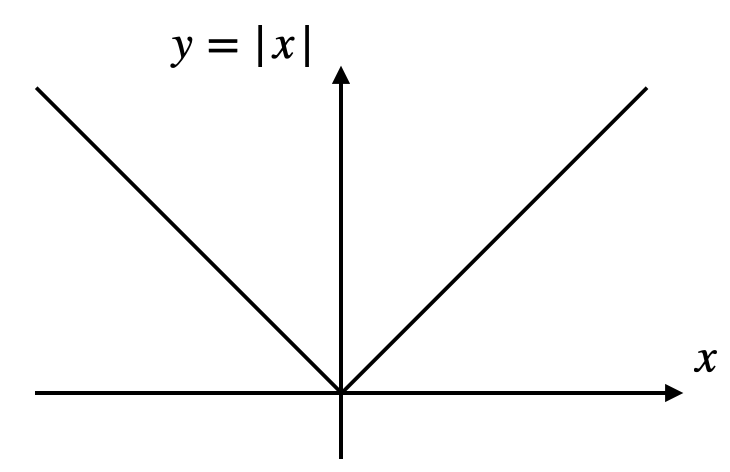
\includegraphics[width=50mm]{calculus4/abs.png}
 \end{center}
\end{figure}

直感的には, $0$で接線が引けないからである. 

\end{frame}


%%%%%%%%%%%%%%%%%%%%%%%%%%%%%%%%%%%%%%%%%%%%%%%%%%%%%%%%%%%%%%%%%%%%%%%%%%%%%%%%%%%%%%%
%%%%%%%%%%%%%%%%%%%%%%%%%%%%%%%%%%%%%%%%%%%%%%%%%%%%%%%%%%%%%%%%%%%%%%%%%%%%%%%%%%%%%%


\begin{frame}
\frametitle{導関数の非存在}


$f(x)=|x|$が$0$で微分不可能であることを確かめる. 
極限
$$
\lim_{h\to 0} \frac{f(a+h)-f(a)}{h}
$$
が存在すれば, 右極限と左極限
$$
\lim_{h\to +0} \frac{f(a+h)-f(a)}{h}, \ \ \ \lim_{h\to -0} \frac{f(a+h)-f(a)}{h}
$$
が存在して, それらは等しいはずである. 
そこで$a=0$とすると
\begin{align*}
\lim_{h\to +0} \frac{f(0+h)-f(0)}{h} & = 
\lim_{h\to +0} \frac{|h|-0}{h}=\lim_{h\to +0} \frac{h}{h}=1 \\
\lim_{h\to -0} \frac{f(0+h)-f(0)}{h} & = 
\lim_{h\to -0} \frac{|h|-0}{h}=\lim_{h\to +0} \frac{-h}{h}=-1
\end{align*}
であるから, 右極限と左極限は一致しない. 
\end{frame}



%%%%%%%%%%%%%%%%%%%%%%%%%%%%%%%%%%%%%%%%%%%%%%%%%%%%%%%%%%%%%%%%%%%%%%%%%%%%%%%%%%%%%%%
%%%%%%%%%%%%%%%%%%%%%%%%%%%%%%%%%%%%%%%%%%%%%%%%%%%%%%%%%%%%%%%%%%%%%%%%%%%%%%%%%%%%%%


\begin{frame}
\frametitle{導関数の計算}


\begin{Prob}
$(3x^2+5)(x^3+x)$の導関数を(1)展開してから計算, (2)積の微分公式を用いて計算, の2通りで求め, 答えが一致することを確かめよ. 
\end{Prob}


\begin{Prob}
$\frac{1}{x}$, $\frac{1}{x^2}$, $\frac{1}{x^3}$の導関数を計算せよ. 
\end{Prob}

\begin{Prob}
$\frac{x}{x+1}-(x+1)(x^2-4)$の導関数を計算せよ. 
\end{Prob}


\end{frame}


%%%%%%%%%%%%%%%%%%%%%%%%%%%%%%%%%%%%%%%%%%%%%%%%%%%%%%%%%%%%%%%%%%%%%%%%%%%%%%%%%%%%%%%
%%%%%%%%%%%%%%%%%%%%%%%%%%%%%%%%%%%%%%%%%%%%%%%%%%%%%%%%%%%%%%%%%%%%%%%%%%%%%%%%%%%%%%


\begin{frame}
\frametitle{定理\ref{微分定理}(2)の証明 (発展)}

公式$(f(x)g(x))'=f'(x)g(x)+f(x)g'(x)$を証明する. 
$$
(f(x)g(x))' = \lim_{h \to 0} \frac{f(x+h)g(x+h)-f(x)g(x)}{h}
$$
であり, 
\begin{align*}
& \frac{f(x+h)g(x+h)-f(x)g(x)}{h} \\
=& 
\frac{f(x+h)g(x+h)-f(x)g(x+h)}{h}
+
\frac{f(x)g(x+h)-f(x)g(x)}{h} \\
=& 
\frac{f(x+h)-f(x)}{h}g(x+h)
+
f(x)\frac{g(x+h)-g(x)}{h} \\
& \hspace{-4mm} \xrightarrow{h \to 0} 
f'(x)g(x)+f(x)g'(x). 
\end{align*}

\end{frame}



%%%%%%%%%%%%%%%%%%%%%%%%%%%%%%%%%%%%%%%%%%%%%%%%%%%%%%%%%%%%%%%%%%%%%%%%%%%%%%%%%%%%%%%
%%%%%%%%%%%%%%%%%%%%%%%%%%%%%%%%%%%%%%%%%%%%%%%%%%%%%%%%%%%%%%%%%%%%%%%%%%%%%%%%%%%%%%


\begin{frame}
\frametitle{定理\ref{微分定理}(3)の証明 (発展)}

公式$\Big(\frac{f(x)}{g(x)}\Big)'=\frac{f'(x)g(x)-f(x)g'(x)}{g(x)^2}$を証明する. 
$$
\Big(\frac{f(x)}{g(x)}\Big)'= \lim_{h \to 0} \Big(\frac{f(x+h)}{g(x+h)} - \frac{f(x)}{g(x)}\Big) \frac{1}{h}
$$
であり, 
\begin{align*}
&\Big(\frac{f(x+h)}{g(x+h)} - \frac{f(x)}{g(x)}\Big) \frac{1}{h} \\
=& 
\frac{f(x+h)g(x)-f(x)g(x+h)}{g(x+h)g(x)} \frac{1}{h} \\
=& 
\Big(
\frac{f(x+h)g(x)-f(x)g(x)}{h}- \frac{f(x)g(x+h)-f(x)g(x)}{h}
\Big) \frac{1}{g(x)g(x+h)}
\end{align*}

\end{frame}


%%%%%%%%%%%%%%%%%%%%%%%%%%%%%%%%%%%%%%%%%%%%%%%%%%%%%%%%%%%%%%%%%%%%%%%%%%%%%%%%%%%%%%%
%%%%%%%%%%%%%%%%%%%%%%%%%%%%%%%%%%%%%%%%%%%%%%%%%%%%%%%%%%%%%%%%%%%%%%%%%%%%%%%%%%%%%%


\begin{frame}
\frametitle{定理\ref{微分定理}(3)の証明 (発展)}


\begin{align*}
=& 
\Big(
\frac{f(x+h)-f(x)}{h} g(x)- f(x)\frac{g(x+h)-g(x)}{h}
\Big) \frac{1}{g(x)g(x+h)}
\\
& \hspace{-4mm} \xrightarrow{h \to 0} 
\frac{f'(x)g(x)-f(x)g'(x)}{g(x)^2}
\end{align*}

別証明として, 比較的簡単な$\Big(\frac{1}{g(x)}\Big)'=-\frac{g'(x)}{g(x)^2}$をまず示し, 
次に積の微分公式を$\frac{f(x)}{g(x)}=f(x) \frac{1}{g(x)}$に使うことで証明することも出来る. 

\end{frame}


%%%%%%%%%%%%%%%%%%%%%%%%%%%%%%%%%%%%%%%%%%%%%%%%%%%%%%%%%%%%%%%%%%%%%%%%%%%%%%%%%%%%%%%
%%%%%%%%%%%%%%%%%%%%%%%%%%%%%%%%%%%%%%%%%%%%%%%%%%%%%%%%%%%%%%%%%%%%%%%%%%%%%%%%%%%%%%%




\section{今日のまとめ}
\begin{frame}
\frametitle{まとめ}   


\begin{enumerate}
\item 平均変化率, 微分係数, 接線の傾き
\item 導関数, 導関数の性質
\end{enumerate} 


\end{frame}


\section{講義概要}


\begin{frame}
\frametitle{今日の内容}



\begin{enumerate}
\item 三角関数, 指数関数, 対数関数の微分,
\item 合成関数の微分, 対数微分
\end{enumerate} 



\end{frame}





%%%%%%%%%%%%%%%%%%%%%%%%%%%%%%%%%%%%%%%%%%%%%%%%%%%%%%%%%%%%%%%%%%%%%%%%%%%%%%%%%%%%%%%
%%%%%%%%%%%%%%%%%%%%%%%%%%%%%%%%%%%%%%%%%%%%%%%%%%%%%%%%%%%%%%%%%%%%%%%%%%%%%%%%%%%%%%%

\section{三角関数の微分}

\begin{frame}
\frametitle{三角関数の微分}


\vspace{-4mm}

三角関数の微分を議論するために必要な準備を行う. 

\vspace{-1mm}

\begin{Thm} \label{準備}
\begin{enumerate}
\item $\displaystyle\lim_{x \to 0} \frac{\sin x}{x}=1$, 
\item  $\displaystyle \lim_{x \to 0} \frac{1-\cos x}{x}=0$. 
\end{enumerate}
\end{Thm}
弧度法において, $x$が弧の長さであることから$0<x<\pi/2$において次の不等式が成立する. 
(扇形と底辺を共有する2つの三角形の面積を比較しても良い.)
\vspace{-6mm}

 \begin{figure}[htbp]
 \begin{center} 
  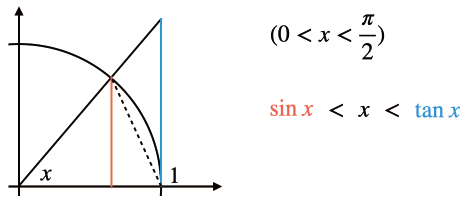
\includegraphics[width=65mm]{calculus5/sintan.png}
 \end{center}
\end{figure}

\vspace{-10mm}

\end{frame}





%%%%%%%%%%%%%%%%%%%%%%%%%%%%%%%%%%%%%%%%%%%%%%%%%%%%%%%%%%%%%%%%%%%%%%%%%%%%%%%%%%%%%%%
%%%%%%%%%%%%%%%%%%%%%%%%%%%%%%%%%%%%%%%%%%%%%%%%%%%%%%%%%%%%%%%%%%%%%%%%%%%%%%%%%%%%%%%


\begin{frame}
\frametitle{定理\ref{準備}\ctext{1}の証明}

$0<x<\pi/2$において
\begin{itemize}
\item $\sin x < x$より, $\frac{\sin x}{x}<1$. 
\item $x < \tan x=\frac{\sin x}{\cos x}$より, $\cos x < \frac{\sin x}{x}$.   
\end{itemize}
纏めると
$$
\cos x < \frac{\sin x}{x} < 1. 
$$
$x \to +0$なる極限をとると
$$
\lim_{x \to +0} \cos x \le \lim_{x \to +0} \frac{\sin x}{x} \le \lim_{x \to +0} 1. 
$$
これより, $\displaystyle\lim_{x \to +0} \frac{\sin x}{x}=1$. (挟み撃ちの定理)\\
\ \\

同様の議論で左極限も$\displaystyle\lim_{x \to -0} \frac{\sin x}{x}=1$.  

\end{frame}



%%%%%%%%%%%%%%%%%%%%%%%%%%%%%%%%%%%%%%%%%%%%%%%%%%%%%%%%%%%%%%%%%%%%%%%%%%%%%%%%%%%%%%%
%%%%%%%%%%%%%%%%%%%%%%%%%%%%%%%%%%%%%%%%%%%%%%%%%%%%%%%%%%%%%%%%%%%%%%%%%%%%%%%%%%%%%%%


\begin{frame}
\frametitle{定理\ref{準備}\ctext{2}の証明}

$\sin^2x +\cos^2 x=1$より
$$
\frac{1-\cos x}{x}
=
\frac{1-\cos ^2x}{x(1+\cos x)}
=
\frac{\sin ^2x}{x(1+\cos x)}
=
\frac{\sin x}{x}
\frac{\sin x}{1+\cos x}
$$
であるから 
$$
\lim_{x \to 0} \frac{1-\cos x}{x}=
\lim_{x \to 0} (\frac{\sin x}{x}
\frac{\sin x}{1+\cos x})
=1 \cdot \frac{0}{1+1}=0. 
$$

\end{frame}




%%%%%%%%%%%%%%%%%%%%%%%%%%%%%%%%%%%%%%%%%%%%%%%%%%%%%%%%%%%%%%%%%%%%%%%%%%%%%%%%%%%%%%%
%%%%%%%%%%%%%%%%%%%%%%%%%%%%%%%%%%%%%%%%%%%%%%%%%%%%%%%%%%%%%%%%%%%%%%%%%%%%%%%%%%%%%%%


\begin{frame}
\frametitle{三角関数の微分}



\begin{Thm} \label{三角関数微分}
\begin{enumerate}
\item $(\sin x)'=\cos x$,
\item  $(\cos x)' = -\sin x$,
\item $(\tan x)'=\frac{1}{\cos^2 x}$. 
\end{enumerate}
\end{Thm}

三角関数の加法定理を思い出しておく. 
\begin{itemize}
\item $\sin(\alpha+\beta)=\sin \alpha \cos \beta + \cos \alpha \sin \beta$
\item $\cos(\alpha+\beta)=\cos \alpha \cos \beta - \sin \alpha \sin \beta$
\end{itemize}

\end{frame}
\begin{slide}{加法定理の図的な説明}
%\begin{eqnarray}
%\sin(A+B) &=& \sin{A}\cos{B} + \sin{B}\cos{A} \\
%\sin(A-B) &=& \sin{A}\cos{B} - \sin{B}\cos{A} \\
%\cos(A+B) &=& \cos{A}\cos{B}-\sin{A}\sin{B} \\
%\cos(A-B)&=&\cos{A}\cos{B}+\sin{A}\sin{B}
%\end{eqnarray}
\begin{figure}[h]                                                                      
\centering
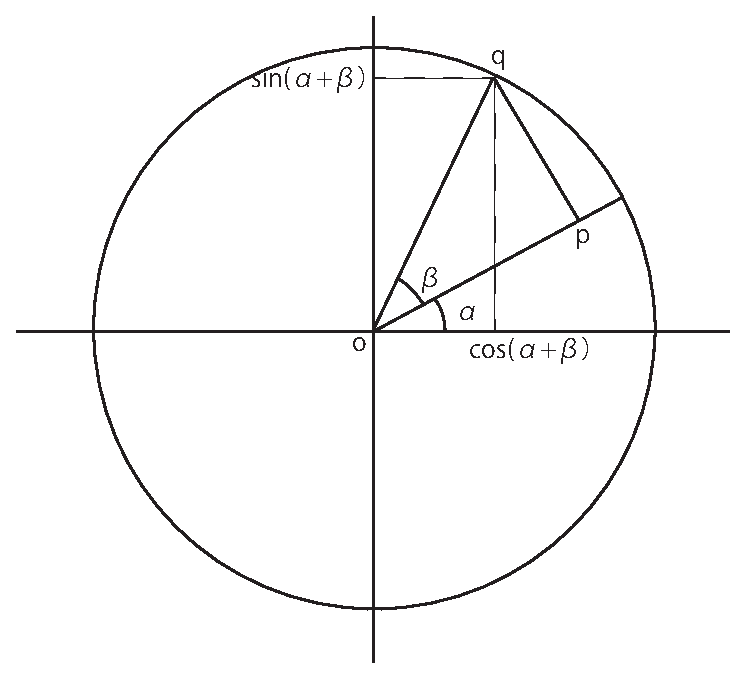
\includegraphics[width=3cm]{calculus5/add.eps}
%\caption{加法定理の図解}
%\label{fig:additive}
\end{figure}
\begin{equation}
\overrightarrow{op} = \cos{\beta}(\cos{\alpha}, \sin{\alpha})
\end{equation}
であり、$\overrightarrow{pq}$は$\overrightarrow{op}$に直交して長さが$\sin{\beta}$であるため
\begin{equation}
\overrightarrow{pq} = \sin{\beta}(-\sin{\alpha}, \cos{\alpha})
\end{equation}
となるため$\overrightarrow{oq}$は
\begin{eqnarray}
\overrightarrow{oq} &=& \overrightarrow{op}+\overrightarrow{pq}\nonumber \\
&=& (\cos{\alpha}\cos{\beta} - \sin{\alpha}\sin{\beta}, \sin{\alpha}\cos{\beta}+\sin{\beta}\cos{\alpha})
\end{eqnarray}
となり、加法定理を与える。
\end{slide}


%%%%%%%%%%%%%%%%%%%%%%%%%%%%%%%%%%%%%%%%%%%%%%%%%%%%%%%%%%%%%%%%%%%%%%%%%%%%%%%%%%%%%%%
%%%%%%%%%%%%%%%%%%%%%%%%%%%%%%%%%%%%%%%%%%%%%%%%%%%%%%%%%%%%%%%%%%%%%%%%%%%%%%%%%%%%%%%


\begin{frame}
\frametitle{定理\ref{三角関数微分}\ctext{1}の証明}

加法定理より
\begin{align*}
\sin(x +h)-\sin x & = \sin x \cos h + \cos x \sin h -\sin x \\
& =  \cos x \sin h + \sin x( \cos h-1)
\end{align*}
であるから
\begin{align*}
(\sin x)' &= \lim_{h \to 0} \frac{\sin(x +h)-\sin x}{h} \\
& =  \lim_{h \to 0} (\cos x \frac{\sin h}{h} + \sin x \frac{\cos h-1}{h}) \\
& =\cos x \cdot 1 + \sin x \cdot 0 \\
& = \cos x. 
\end{align*}
\end{frame}


%%%%%%%%%%%%%%%%%%%%%%%%%%%%%%%%%%%%%%%%%%%%%%%%%%%%%%%%%%%%%%%%%%%%%%%%%%%%%%%%%%%%%%%
%%%%%%%%%%%%%%%%%%%%%%%%%%%%%%%%%%%%%%%%%%%%%%%%%%%%%%%%%%%%%%%%%%%%%%%%%%%%%%%%%%%%%%%


\begin{frame}
\frametitle{定理\ref{三角関数微分}\ctext{2}の証明}

加法定理より
\begin{align*} 
\cos(x +h)-\cos x & = \cos x \cos h - \sin x \sin h -\cos x \\
& =  \cos x (\cos h-1) - \sin x \sin h
\end{align*}
であるから
\begin{align*}
(\cos x)' &= \lim_{h \to 0} \frac{\cos(x +h)-\cos x}{h} \\
& =  \lim_{h \to 0} (\cos x \frac{\cos h-1}{h} - \sin x \frac{\sin h}{h}) \\
& =\cos x \cdot 0 - \sin x \cdot 1 \\
& = -\sin x. 
\end{align*}
\end{frame}


%%%%%%%%%%%%%%%%%%%%%%%%%%%%%%%%%%%%%%%%%%%%%%%%%%%%%%%%%%%%%%%%%%%%%%%%%%%%%%%%%%%%%%%
%%%%%%%%%%%%%%%%%%%%%%%%%%%%%%%%%%%%%%%%%%%%%%%%%%%%%%%%%%%%%%%%%%%%%%%%%%%%%%%%%%%%%%%


\begin{frame}
\frametitle{定理\ref{三角関数微分}\ctext{3}の証明}

商の微分公式より
\begin{align*} 
(\tan x)' &= \Big( \frac{\sin x}{\cos x} \Big)' \\
&= \frac{(\sin x)'\cos x - \sin x (\cos x)'}{\cos^2 x} \\
&= \frac{\cos^2 x + \sin^2 x}{\cos^2 x} \\
&= \frac{1}{\cos^2 x}. 
\end{align*}

\end{frame}


%%%%%%%%%%%%%%%%%%%%%%%%%%%%%%%%%%%%%%%%%%%%%%%%%%%%%%%%%%%%%%%%%%%%%%%%%%%%%%%%%%%%%%%
%%%%%%%%%%%%%%%%%%%%%%%%%%%%%%%%%%%%%%%%%%%%%%%%%%%%%%%%%%%%%%%%%%%%%%%%%%%%%%%%%%%%%%%


\begin{frame}
\frametitle{三角関数の微分}

\begin{Prob}
次の関数の導関数を求めよ. 
\begin{enumerate}
\item $\sin^2 x$
\item $\sin^3 x$
\item $\sin x \cos x$
\item $\frac{\cos x}{x}$
\end{enumerate}
\end{Prob}

\end{frame}


%%%%%%%%%%%%%%%%%%%%%%%%%%%%%%%%%%%%%%%%%%%%%%%%%%%%%%%%%%%%%%%%%%%%%%%%%%%%%%%%%%%%%%%
%%%%%%%%%%%%%%%%%%%%%%%%%%%%%%%%%%%%%%%%%%%%%%%%%%%%%%%%%%%%%%%%%%%%%%%%%%%%%%%%%%%%%%%

\section{指数関数と対数関数の微分}

\begin{frame}
\frametitle{ネイピア数}

ネイピア数$e=2.71828\dots$に関して, 次が成立する.  
$$
e=\lim_{x \to +\infty} \Big(1+\frac{1}{x}\Big)^x = \lim_{x \to -\infty} \Big(1+\frac{1}{x}\Big)^x. 
$$
これは$\displaystyle e=\lim_{x\to 0}(1+x)^\frac{1}{x}$とも同値である. \\
\ \\

いくつか計算してみると
\begin{align*}
(1+\frac{1}{10})^{10}&=2.5937\dots, \ \ \ 
(1+\frac{1}{100})^{100}=2.7048\dots, \\
(1+\frac{1}{1000})^{1000}&=2.7169\dots, \ \ \ 
(1+\frac{1}{10000})^{10000}=2.7181\dots, 
\end{align*}

\end{frame}




%%%%%%%%%%%%%%%%%%%%%%%%%%%%%%%%%%%%%%%%%%%%%%%%%%%%%%%%%%%%%%%%%%%%%%%%%%%%%%%%%%%%%%%
%%%%%%%%%%%%%%%%%%%%%%%%%%%%%%%%%%%%%%%%%%%%%%%%%%%%%%%%%%%%%%%%%%%%%%%%%%%%%%%%%%%%%%%



\begin{frame}
\frametitle{準備}

指数関数と対数関数の微分を議論するために必要な準備を行う. 

\begin{Thm} \label{準備2}
\begin{enumerate}
\item $\displaystyle \lim_{h \to 0} \frac{e^h-1}{h}=1$, 
\item  $\displaystyle \lim_{h \to 0} \frac{\log(1+h)}{h}=1$. 
\end{enumerate}
\end{Thm}


\end{frame}



%%%%%%%%%%%%%%%%%%%%%%%%%%%%%%%%%%%%%%%%%%%%%%%%%%%%%%%%%%%%%%%%%%%%%%%%%%%%%%%%%%%%%%%
%%%%%%%%%%%%%%%%%%%%%%%%%%%%%%%%%%%%%%%%%%%%%%%%%%%%%%%%%%%%%%%%%%%%%%%%%%%%%%%%%%%%%%%


\begin{frame}
\frametitle{定理\ref{準備2}の証明}

まず\ctext{2}を示す. 
\begin{align*} 
\lim_{h \to 0} \frac{\log(1+h)}{h} & = \lim_{h \to 0} \log(1+h)^{\frac{1}{h}} \\
& = \log \big( \lim_{h \to 0} (1+h)^{\frac{1}{h}} \big) \ \ \ (\text{対数関数の連続性})\\
& = \log e = 1. 
\end{align*}
次に\ctext{1}を示す. 
まず$t=e^h-1$とおくと, $h\to 0$のとき$t\to0$である. 
また$e^h=1+t$より$h=\log (1+t)$であるから, \ctext{2}より
$$
\lim_{h \to 0} \frac{e^h-1}{h}=\lim_{t \to 0} \frac{t}{\log(1+t)}=1. 
$$

\end{frame}


%%%%%%%%%%%%%%%%%%%%%%%%%%%%%%%%%%%%%%%%%%%%%%%%%%%%%%%%%%%%%%%%%%%%%%%%%%%%%%%%%%%%%%%
%%%%%%%%%%%%%%%%%%%%%%%%%%%%%%%%%%%%%%%%%%%%%%%%%%%%%%%%%%%%%%%%%%%%%%%%%%%%%%%%%%%%%%%


\begin{frame}
\frametitle{指数関数の微分}

 指数関数$e^x$は微分しても不変であるという特殊な性質を持つ. 

\begin{Thm} 
$$(e^x)'=e^x$$
\end{Thm}

定理\ref{準備2}\ctext{1}より
\begin{align*} 
(e^x)' &= \lim_{h\to0}\frac{e^{x+h}-e^x}{h}=\lim_{h\to0}e^x \frac{e^h-1}{h}=e^x\cdot 1 = e^x. 
\end{align*}

微分して不変な関数は$e^x$の定数倍しかないことも知られている. 
つまり微分方程式$f'(x)=f(x)$の解は$f(x)=Ce^x$の形($C$:定数). 
底が$e$でない場合は講義の後半で扱う. 

\end{frame}



%%%%%%%%%%%%%%%%%%%%%%%%%%%%%%%%%%%%%%%%%%%%%%%%%%%%%%%%%%%%%%%%%%%%%%%%%%%%%%%%%%%%%%%
%%%%%%%%%%%%%%%%%%%%%%%%%%%%%%%%%%%%%%%%%%%%%%%%%%%%%%%%%%%%%%%%%%%%%%%%%%%%%%%%%%%%%%%


\begin{frame}
\frametitle{対数関数の微分}


\begin{Thm} 
$$(\log x)'=\frac{1}{x}$$
\end{Thm}

定理\ref{準備2}\ctext{2}より \vspace{-2mm}
\begin{align*} 
(\log x)' &= \lim_{h\to0}\frac{\log(x+h)-\log x}{h} \\
&= \lim_{h\to0}\frac{1}{h} \log \frac{x+h}{x} = \lim_{h\to0}\frac{1}{h} \log (1+\frac{h}{x}) \\
&= \lim_{t\to0}\frac{1}{tx} \log (1+t) = \lim_{t\to0}\frac{1}{x} \frac{\log (1+t)}{t} \\
&=\frac{1}{x}\cdot 1=\frac{1}{x}. 
\end{align*}

途中で$t=\frac{h}{x}$なる変数変換をしている. 

\end{frame}



%%%%%%%%%%%%%%%%%%%%%%%%%%%%%%%%%%%%%%%%%%%%%%%%%%%%%%%%%%%%%%%%%%%%%%%%%%%%%%%%%%%%%%%
%%%%%%%%%%%%%%%%%%%%%%%%%%%%%%%%%%%%%%%%%%%%%%%%%%%%%%%%%%%%%%%%%%%%%%%%%%%%%%%%%%%%%%%

\section{合成関数の微分}

\begin{frame}
\frametitle{合成関数の微分}

関数$g:D \rightarrow \R, x\mapsto g(x)$と$f:E\rightarrow \R, y\mapsto f(y)$で, 像$\mathrm{Im}g$が$E$に含まれるものに対して, 
\underline{合成関数}
$$
f\circ g:D \longrightarrow \R, \ \ \ x \mapsto f(g(x))
$$
を考えることができる. 
これは合成写像の特別な場合であるが, 関数であることを強調して$f(g(x))$という記号を使うことが多い. 


\end{frame}


%%%%%%%%%%%%%%%%%%%%%%%%%%%%%%%%%%%%%%%%%%%%%%%%%%%%%%%%%%%%%%%%%%%%%%%%%%%%%%%%%%%%%%%
%%%%%%%%%%%%%%%%%%%%%%%%%%%%%%%%%%%%%%%%%%%%%%%%%%%%%%%%%%%%%%%%%%%%%%%%%%%%%%%%%%%%%%%


\begin{frame}
\frametitle{合成関数の微分}


\begin{Thm} \label{合成関数}
$f(y)$, $g(x)$が微分可能であれば, 合成関数$f(g(x))$も微分可能で, 
$$
(f(g(x)))'=f'(g(x))g'(x)
$$
\end{Thm}
$y=g(x)$, $z=f(y)$とすれば, 
$$
\frac{dz}{dx}=\frac{dz}{dy} \frac{dy}{dx}
$$
と表現することも可能. 
導関数は分数ではないが, 形式的に約分できると思うと, 右辺から左辺が得られる. 

\end{frame}


%%%%%%%%%%%%%%%%%%%%%%%%%%%%%%%%%%%%%%%%%%%%%%%%%%%%%%%%%%%%%%%%%%%%%%%%%%%%%%%%%%%%%%%
%%%%%%%%%%%%%%%%%%%%%%%%%%%%%%%%%%%%%%%%%%%%%%%%%%%%%%%%%%%%%%%%%%%%%%%%%%%%%%%%%%%%%%%


\begin{frame}
\frametitle{定理\ref{合成関数}の大雑把な証明}


十分小さな$h$に関して$k=g(x+h)- g(x)\ne 0$を仮定する. 
$g(x)$の連続性より, $h \to 0$で$k\to 0$に注意すると
\begin{align*} 
(f(g(x)))' &= \lim_{h\to 0}\frac{f(g(x+h))-f(g(x))}{h} \\
& =  \lim_{h\to 0}\frac{f(g(x+h))-f(g(x))}{g(x+h)-g(x)} \frac{g(x+h)-g(x)}{h} \\
& =  \lim_{h\to 0}\frac{f(g(x)+k)-f(g(x))}{k} \frac{g(x+h)-g(x)}{h} \\
& =f'(g(x))g'(x)
\end{align*}
$\lim_{h\to 0}g(x+h) - g(x) = 0$の場合、仮定が成立しないので, 厳密な証明としては不十分. 

\end{frame}


%%%%%%%%%%%%%%%%%%%%%%%%%%%%%%%%%%%%%%%%%%%%%%%%%%%%%%%%%%%%%%%%%%%%%%%%%%%%%%%%%%%%%%%
%%%%%%%%%%%%%%%%%%%%%%%%%%%%%%%%%%%%%%%%%%%%%%%%%%%%%%%%%%%%%%%%%%%%%%%%%%%%%%%%%%%%%%%


%\begin{frame}
%\frametitle{定理\ref{合成関数}の証明 (発展)}
%
%
%一般に, $f(x)$が$a$で微分可能なとき, 関数$\delta(x)$で$\displaystyle \lim_{x\to a}\delta(x)=0$なるものが存在して
%$$
%f(x)=f(a)+f'(a)(x-a)+\delta(x)(x-a)
%$$
%と書くことができる. 
%$a$を$g(x)$, $x$を$g(x+h)$に置き換えることで
%\begin{align*} 
%f(g(x+h))=& f(g(x))+f'(g(x))(g(x+h)-g(x)) \\
%&+\delta(g(x+h))(g(x+h)-g(x)) 
%\end{align*}
%これより
%\begin{align*} 
%\frac{f(g(x+h))-f(g(x))}{h}= & f'(g(x))\frac{g(x+h)-g(x)}{h} \\
%&+\delta(g(x+h))\frac{g(x+h)-g(x)}{h}. 
%\end{align*}
%$h\to 0$として, 第一項は$f'(g(x))g'(x)$に第二項は$0$に収束する. 
%\end{frame}
\begin{slide}{定理\ref{合成関数}の証明 2}
$y=g(x)$の微分は
\begin{equation}
g(x)'= \lim_{h\to 0} \frac{g(x+h) - g(x)}{h} \nonumber
\end{equation}
なので, $g(x+h)$は微分の誤差を表す関数
$p(x) \quad \lim_{x\to 0} p(x+h) = 0$を用いて以下のように書ける。
$p(x+h)h$は$p(x+h)$と書いたほうが自然であるが、後で$h$で割りたいので、このように定義しておく。
\begin{equation}
g(x+h) = g(x) + g(x)'h + p(x+h)h\nonumber
\end{equation}
図で書くと以下である。
\begin{figure}[h]
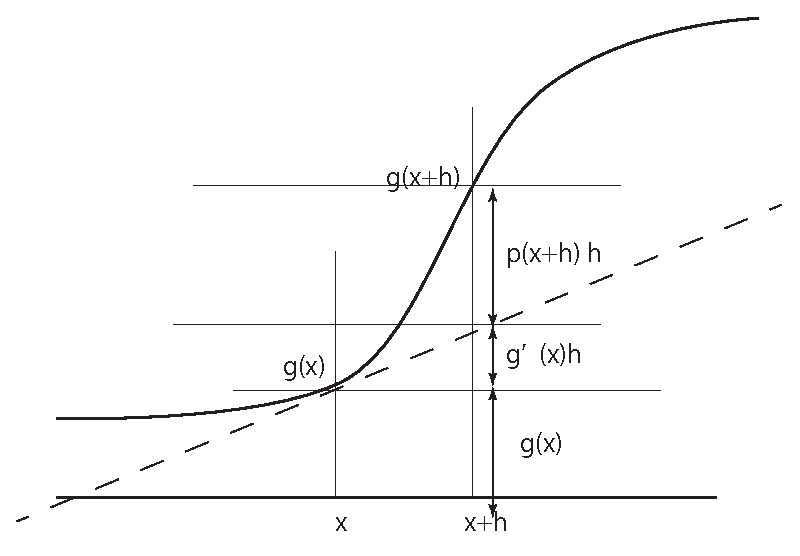
\includegraphics[width=4cm]{calculus5/gosei.eps}
\end{figure}
\end{slide}
\begin{slide}{定理\ref{合成関数}の証明2}
同様に$f(y)$についても微分の誤差を表す関数$q(y) \quad \lim_{u\to 0} q(y+u) = 0$を用い
\begin{equation}
f(y+u) = f(y) + f(y)'u+q(y+u)u \nonumber 
\end{equation}
であり$u = g(x+h) - g(x) = (g'(x) + p(x+h)) h$なので、以下のように求められる。
\begin{eqnarray}
(f(g(x)))' &=& \lim_{h\to 0} \frac{f(y+u) - f(y)}{h}  \nonumber \\
&=& \lim_{h\to 0} \frac{(f'(y) + q(y+u)) u}{h} \nonumber \\
&=& \lim_{h\to 0} \frac{(f'(y) + q(y+u))(g'(x) + p(x+h))\cancel{h}}{\cancel{h}} \nonumber \\
&=& \lim_{h\to 0}(f'(y) + q(y+u))(g'(x) + p(x+h)) = f'(y) g'(x) \nonumber 
\end{eqnarray}
\end{slide}


%%%%%%%%%%%%%%%%%%%%%%%%%%%%%%%%%%%%%%%%%%%%%%%%%%%%%%%%%%%%%%%%%%%%%%%%%%%%%%%%%%%%%%%
%%%%%%%%%%%%%%%%%%%%%%%%%%%%%%%%%%%%%%%%%%%%%%%%%%%%%%%%%%%%%%%%%%%%%%%%%%%%%%%%%%%%%%%


\begin{frame}
\frametitle{合成関数の微分}


$\big((5x^2+3)^9\big)'$を計算することを考える. 
勿論, 展開してから微分しても良いが, 計算が面倒である. \\
\ \\

一方で, $f(y)=y^9$と$g(x)=5x^2+3$を用いて$f(g(x))=(5x^2+3)^9$と書けることから
\begin{align*} 
\big((5x^2+3)^9\big)' &= (y^9)'  \ \ \ \ \ \ \ \ \ \ (y=g(x)\text{とおいた})\\
& =9y^8 \cdot y' \\
&=9(5x^2+3)^8 \cdot 10x \\
&= 90x(5x^2+3)^8. 
\end{align*}
\end{frame}



%%%%%%%%%%%%%%%%%%%%%%%%%%%%%%%%%%%%%%%%%%%%%%%%%%%%%%%%%%%%%%%%%%%%%%%%%%%%%%%%%%%%%%%
%%%%%%%%%%%%%%%%%%%%%%%%%%%%%%%%%%%%%%%%%%%%%%%%%%%%%%%%%%%%%%%%%%%%%%%%%%%%%%%%%%%%%%%


\begin{frame}
\frametitle{合成関数の微分}


$(e^{3x^2+7})'$を計算することを考える. \\
\ \\

$f(y)=e^y$と$g(x)=3x^2+7$を用いて$f(g(x))=e^{3x^2+7}$と書けることから
\begin{align*} 
(e^{3x^2+7})' &= (e^y)'  \ \ \ \ \ \ \ \ \ \ (y=g(x)\text{とおいた})\\
& =e^y \cdot y' \\
&=e^{3x^2+7} \cdot 6x \\
&= 6x e^{3x^2+7}. 
\end{align*}


\end{frame}



%%%%%%%%%%%%%%%%%%%%%%%%%%%%%%%%%%%%%%%%%%%%%%%%%%%%%%%%%%%%%%%%%%%%%%%%%%%%%%%%%%%%%%%
%%%%%%%%%%%%%%%%%%%%%%%%%%%%%%%%%%%%%%%%%%%%%%%%%%%%%%%%%%%%%%%%%%%%%%%%%%%%%%%%%%%%%%%


\begin{frame}
\frametitle{合成関数の微分}


\begin{Prob}
次の関数の導関数を求めよ. 
\begin{enumerate}
\item $(x^2+x+1)^9$, 
\item $\sin^3 x$, 
\item $\cos( x^2)$, 
\item $(x^2+1)^2(2x^3-1)^4$. 
%\item $\cos \frac{1}{x}$, 演習に
%\item $\cos^3(2x+1)$. 
\end{enumerate}
\end{Prob}


\end{frame}




%%%%%%%%%%%%%%%%%%%%%%%%%%%%%%%%%%%%%%%%%%%%%%%%%%%%%%%%%%%%%%%%%%%%%%%%%%%%%%%%%%%%%%%
%%%%%%%%%%%%%%%%%%%%%%%%%%%%%%%%%%%%%%%%%%%%%%%%%%%%%%%%%%%%%%%%%%%%%%%%%%%%%%%%%%%%%%%



\section{一般の指数関数の微分}


\begin{frame}
\frametitle{一般の指数関数の微分}


\begin{Thm} 
$a>0$に関して
$$(a^x)'=a^x \log a$$
\end{Thm}

$a=e^{\log a}$に注意すると
$$
a^x=(e^{\log a})^x=e^{x \log a}
$$
であるから, 
$f(y)=e^y$と$g(x)=x \log a$を用いて$f(g(x))=a^x=e^{x \log a}$と書けることから
\begin{align*} 
(a^x)' &= (e^y)'  =e^y \cdot y' =a^x \log a. 
\end{align*}


\end{frame}


%%%%%%%%%%%%%%%%%%%%%%%%%%%%%%%%%%%%%%%%%%%%%%%%%%%%%%%%%%%%%%%%%%%%%%%%%%%%%%%%%%%%%%%
%%%%%%%%%%%%%%%%%%%%%%%%%%%%%%%%%%%%%%%%%%%%%%%%%%%%%%%%%%%%%%%%%%%%%%%%%%%%%%%%%%%%%%%


\section{対数関数の微分の拡張}

\begin{frame}
\frametitle{対数関数の微分の拡張}

$\log x$の定義域は$x>0$であるが, $\log |x|$を考えることで, 定義域を$x\neq 0$なる実数全体に拡張される. 

 \begin{figure}[htbp]
 \begin{center} 
  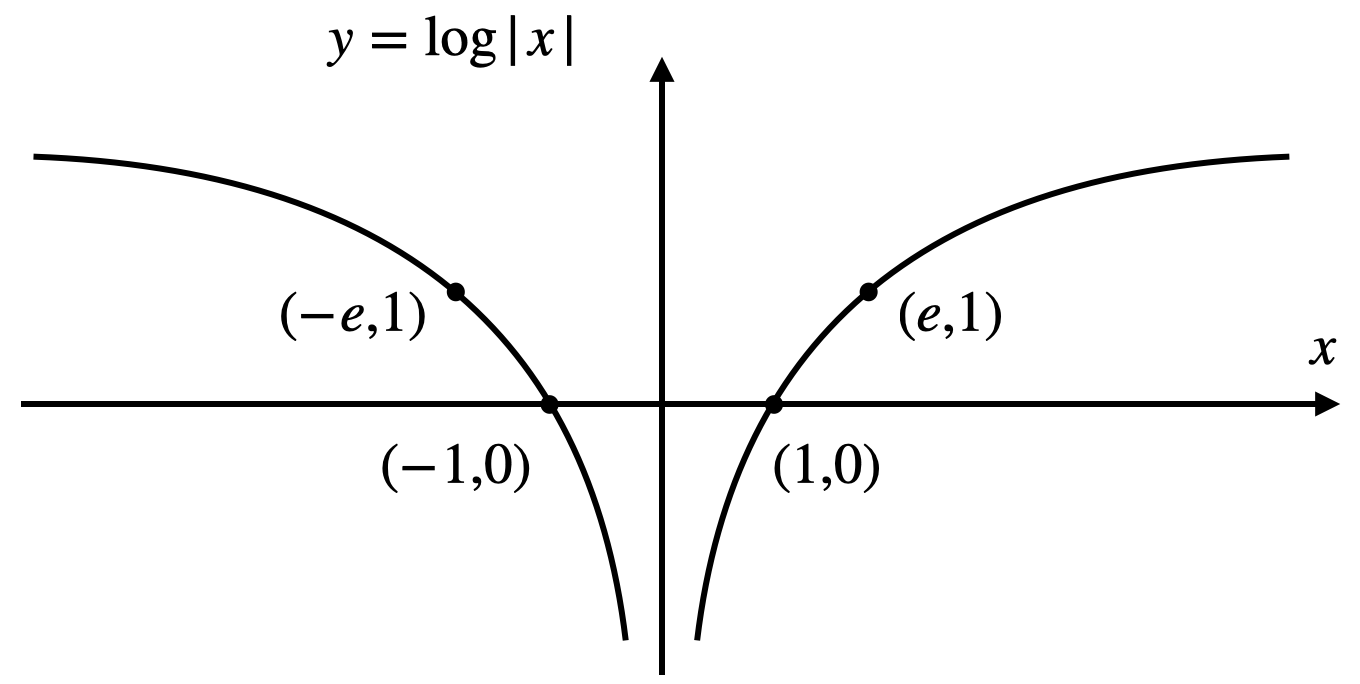
\includegraphics[width=90mm]{calculus5/log_abs.png}
 \end{center}
\end{figure}


\end{frame}


%%%%%%%%%%%%%%%%%%%%%%%%%%%%%%%%%%%%%%%%%%%%%%%%%%%%%%%%%%%%%%%%%%%%%%%%%%%%%%%%%%%%%%%
%%%%%%%%%%%%%%%%%%%%%%%%%%%%%%%%%%%%%%%%%%%%%%%%%%%%%%%%%%%%%%%%%%%%%%%%%%%%%%%%%%%%%%%


\begin{frame}
\frametitle{対数関数の微分の拡張}


\begin{Thm} 
$$(\log |x|)'=\frac{1}{x}$$
\end{Thm}

\begin{itemize}
\item $x>0$の場合
$$
(\log |x|)' = (\log x)'=\frac{1}{x}
$$
\item $x<0$の場合
$$
(\log |x|)' = (\log (-x))'=\frac{1}{-x} \cdot (-1)=\frac{1}{x}. 
$$
\end{itemize}


\end{frame}


%%%%%%%%%%%%%%%%%%%%%%%%%%%%%%%%%%%%%%%%%%%%%%%%%%%%%%%%%%%%%%%%%%%%%%%%%%%%%%%%%%%%%%%
%%%%%%%%%%%%%%%%%%%%%%%%%%%%%%%%%%%%%%%%%%%%%%%%%%%%%%%%%%%%%%%%%%%%%%%%%%%%%%%%%%%%%%%


\section{対数微分}

\begin{frame}
\frametitle{対数微分}



\begin{Thm} \label{対数微分}
微分可能な関数$g(x)$に対して
$$(\log |g(x)|)'=\frac{g'(x)}{g(x)}$$
\end{Thm}

$f(y)=\log |y|$と$g(x)$を用いて$f(g(x))=\log|g(x)|$と書けることから
$$
(\log |g(x)|)'=\frac{1}{g(x)}\cdot g'(x)=\frac{g'(x)}{g(x)}. 
$$
関数の対数を取ってから微分する方法は\underline{対数微分}と呼ばれ, 様々な場面に現れる. 

\end{frame}


%%%%%%%%%%%%%%%%%%%%%%%%%%%%%%%%%%%%%%%%%%%%%%%%%%%%%%%%%%%%%%%%%%%%%%%%%%%%%%%%%%%%%%%
%%%%%%%%%%%%%%%%%%%%%%%%%%%%%%%%%%%%%%%%%%%%%%%%%%%%%%%%%%%%%%%%%%%%%%%%%%%%%%%%%%%%%%%


\begin{frame}
\frametitle{$(x^a)'=ax^{a-1}$}



\begin{Thm} 
$a \in \R$に関して, $x>0$において
$$
(x^a)'=ax^{a-1}.
$$
\end{Thm}
$g(x)=x^a$とすれば
$$
(\log |g(x)|)'= (\log x^a)'= (a \log x)'=\frac{a}{x}. 
$$
定理\ref{対数微分}より
$$
\frac{a}{x}=\frac{g'(x)}{g(x)}=\frac{(x^a)'}{x^a}
$$
であるから
$$
(x^a)'=a x^{a-1}. 
$$
これは対数微分の典型的な応用例. 

\end{frame}


%%%%%%%%%%%%%%%%%%%%%%%%%%%%%%%%%%%%%%%%%%%%%%%%%%%%%%%%%%%%%%%%%%%%%%%%%%%%%%%%%%%%%%%
%%%%%%%%%%%%%%%%%%%%%%%%%%%%%%%%%%%%%%%%%%%%%%%%%%%%%%%%%%%%%%%%%%%%%%%%%%%%%%%%%%%%%%%


\begin{frame}
\frametitle{$(x^a)'=ax^{a-1}$}


具体的に計算すれば
\begin{align*}
(\sqrt{x})' &= (x^{\frac{1}{2}})'=\frac{1}{2}x^{-\frac{1}{2}}= \frac{1}{2 \sqrt{x}}, \\
(\sqrt[3]{x^2})' &= (x^{\frac{2}{3}})'=\frac{2}{3}x^{-\frac{1}{3}}= \frac{2}{3 \sqrt[3]{x}}
\end{align*}

% x^xも対数微分の良い応用例

\end{frame}



%%%%%%%%%%%%%%%%%%%%%%%%%%%%%%%%%%%%%%%%%%%%%%%%%%%%%%%%%%%%%%%%%%%%%%%%%%%%%%%%%%%%%%%
%%%%%%%%%%%%%%%%%%%%%%%%%%%%%%%%%%%%%%%%%%%%%%%%%%%%%%%%%%%%%%%%%%%%%%%%%%%%%%%%%%%%%%%




\section{今日のまとめ}
\begin{frame}
\frametitle{まとめ}   


\begin{enumerate}
\item 三角関数, 指数関数, 対数関数の微分,
\item 合成関数の微分, 対数微分
\end{enumerate} 


\end{frame}

\documentclass[dvipdfmx,cjk,10.2pt]{beamer} 
%\documentclass[dvipdfm,cjk]{beamer} %% オプションは環境や利用するプログラムに
%\documentclass[dvips,cjk]{beamer}   %% よって変える

\usepackage{subfigure}
\usepackage[all]{xy}
\usepackage{wrapfig}

\newcommand{\C}{\mathbb{C}}
\newcommand{\D}{\mathbb{D}}
\newcommand{\R}{\mathbb{R}}
\newcommand{\Q}{\mathbb{Q}}
\newcommand{\Z}{\mathbb{Z}}
\newcommand{\N}{\mathbb{N}}

\newcommand{\Imag}{\mathrm{Im}}
\newcommand{\id}{\mathrm{id}}


\makeatletter
\newcommand\xleftrightarrow[2][]{%
  \ext@arrow 9999{\longleftrightarrowfill@}{#1}{#2}}
\newcommand\longleftrightarrowfill@{%
  \arrowfill@\leftarrow\relbar\rightarrow}
\makeatother

\AtBeginDvi{\special{pdf:tounicode 90ms-RKSJ-UCS2}} %% しおりが文字化けしないように
%\AtBeginDvi{\special{pdf:tounicode EUC-UCS2}}

\setbeamertemplate{navigation symbols}{} %% 右下のアイコンを消す
\setbeamertemplate{theorems}[normal font] %%斜体を直す

\usetheme{CambridgeUS}         %% theme の選択
%\usetheme{Boadilla}           %% Beamer のディレクトリの中の
%\usetheme{Madrid}             %% beamerthemeCambridgeUS.sty を指定
%\usetheme{Antibes}            %% 色々と試してみるといいだろう
%\usetheme{Montpellier}        %% サンプルが beamer\doc に色々とある。
%\usetheme{Berkeley}
%\usetheme{Goettingen}
%\usetheme{Singapore}
%\usetheme{Szeged}

%\usecolortheme{rose}          %% colortheme を選ぶと色使いが変わる
%\usecolortheme{albatross}

%\useoutertheme{shadow}                 %% 箱に影をつける
\usefonttheme{professionalfonts}       %% 数式の文字を通常の LaTeX と同じにする

%\setbeamercovered{transparent}         %% 消えている文字をうっすらと表示する


\theoremstyle{definition}
\setbeamertemplate{theorems}[numbered]  %% 定理に番号をつける
\newtheorem{Thm}{定理}[section]
%\theoremstyle{example}
\newtheorem{Ex}[Thm]{例}
%\newtheorem{exam}[thm]{Example}
\newtheorem{Rem}[Thm]{注意}
\newtheorem{Conj}[Thm]{予想}
\newtheorem{Def}[Thm]{定義}
\newtheorem{Prob}[Thm]{問題}

\setbeamercolor{block title}{fg=blue!70!black, bg=blue!15!white} 
\setbeamercolor{block body}{fg=black, bg=blue!10!white}



\begin{document}
\title{微分・積分 第6回} 
\author{慶応義塾大学}            %% ここに書かれた情報は色々なところに使われるので
\institute[]{総合政策学部・環境情報学部}   %% なるべく設定した方が良い
\date{}



\begin{frame}                  %% \begin{frame}..\end{frame} で 1 枚のスライド
\titlepage                     %% タイトルページ
\end{frame}

%\begin{frame}                  %% 目次 (必要なければ省略)
%\tableofcontents
%\end{frame}






%%%%%%%%%%%%%%%%%%%%%%%%%%%%%%%%%%%%%%%%%%%%%%%%%%%%%%%%%%%%%%%%%%%%%%%%%%%%%%%%%%%%%%%
%%%%%%%%%%%%%%%%%%%%%%%%%%%%%%%%%%%%%%%%%%%%%%%%%%%%%%%%%%%%%%%%%%%%%%%%%%%%%%%%%%%%%%%

\section{講義概要}


\begin{frame}
\frametitle{今日の内容}



\begin{enumerate}
\item 逆写像, 逆関数, 逆関数の微分
\item 逆三角関数, 逆三角関数の微分
\end{enumerate} 



\end{frame}




%%%%%%%%%%%%%%%%%%%%%%%%%%%%%%%%%%%%%%%%%%%%%%%%%%%%%%%%%%%%%%%%%%%%%%%%%%%%%%%%%%%%%%%
%%%%%%%%%%%%%%%%%%%%%%%%%%%%%%%%%%%%%%%%%%%%%%%%%%%%%%%%%%%%%%%%%%%%%%%%%%%%%%%%%%%%%%%


%%%%%%%%%%%%%%%%%%%%%%%%%%%%%%%%%%%%%%%%%%%%%%%%%%%%%%%%%%%%%%%%%%%%%%%%%%%%%%%%%%%%%%%
%%%%%%%%%%%%%%%%%%%%%%%%%%%%%%%%%%%%%%%%%%%%%%%%%%%%%%%%%%%%%%%%%%%%%%%%%%%%%%%%%%%%%%%



\section{逆写像}


\begin{frame}
\frametitle{全射, 単射}

写像$f:X\rightarrow Y$に対して, 
$\Imag f =\{ f(x) \ | \ x \in X\} \subset Y$であった. 
\begin{Def}
\begin{enumerate}
\item $f$が\underline{全射}であるとは$\Imag f = Y$が成立すること. 
つまり「どの$y \in Y$に対しても$x \in X$が存在して$y=f(x)$」. 
\item $f$が\underline{単射}であるとは「$x_1\ne x_2$ならば$f(x_1)\ne f(x_2)$」が成立すること. 
同値な対偶条件は「$f(x_1)= f(x_2)$ならば$x_1= x_2$」.  
\item $f$が\underline{全単射}であるとは, 全射かつ単射であること. 
\end{enumerate}
\end{Def}

例: あみだくじは全単射. 

\vspace{-2mm}

 \begin{figure}[htbp]
 \begin{center} 
  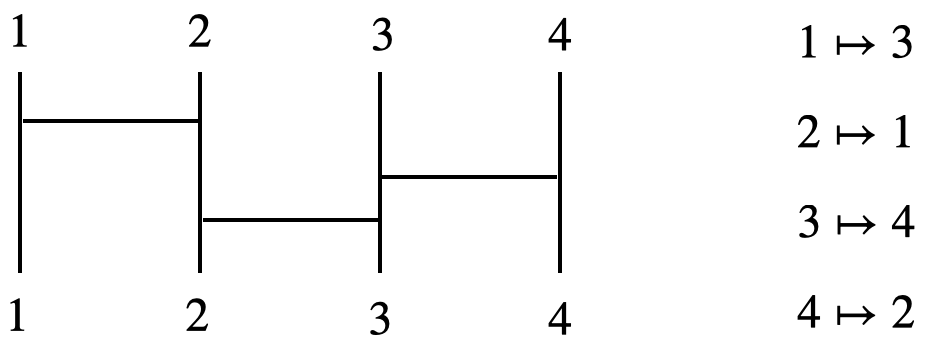
\includegraphics[width=60mm]{amida.png}
 \end{center}
\end{figure}

\vspace{-2mm}


\end{frame}

%%%%%%%%%%%%%%%%%%%%%%%%%%%%%%%%%%%%%%%%%%%%%%%%%%%%%%%%%%%%%%%%%%%%%%%%%%%%%%%%%%%%%%%
%%%%%%%%%%%%%%%%%%%%%%%%%%%%%%%%%%%%%%%%%%%%%%%%%%%%%%%%%%%%%%%%%%%%%%%%%%%%%%%%%%%%%%%



\begin{frame}
\frametitle{逆写像}


\begin{Thm}
写像$f:X\rightarrow Y$が全単射であれば, 写像$g:Y\rightarrow X$が存在して, 
$$
g\circ f = \id, \ \ \ f \circ g = \id
$$
が成立する. 
この$g$を$f$の\underline{逆写像}といい, $f^{-1}$と書く. 
\end{Thm}

実際, 任意の$y \in Y$に対して, $x \in X$で$f(x)=y$なるものが唯一つ存在するので, $g(y)=x$と定義すれば良い. 
\vspace{-4mm}

 \begin{figure}[htbp]
 \begin{center} 
  \includegraphics[width=25mm]{inverse.png}
 \end{center}
\end{figure}

\vspace{-2mm}

特に$X \subset \R$, $Y \subset \R$のときに, 逆写像を逆関数と呼ぶ. 

\end{frame}


%%%%%%%%%%%%%%%%%%%%%%%%%%%%%%%%%%%%%%%%%%%%%%%%%%%%%%%%%%%%%%%%%%%%%%%%%%%%%%%%%%%%%%%
%%%%%%%%%%%%%%%%%%%%%%%%%%%%%%%%%%%%%%%%%%%%%%%%%%%%%%%%%%%%%%%%%%%%%%%%%%%%%%%%%%%%%%%



%\begin{frame}
%\frametitle{逆写像}
%
%
%\begin{Prob}
%あみだくじは全単射$f:\{1,2\dots,n\}\rightarrow \{1,2\dots,n\}$を与えるが, 
%\begin{enumerate}
%\item 2つのあみだくじの合成はあみだくじで与えられるか? 
%\item 逆写像はどう作れば良いか? 
%\end{enumerate}
%\end{Prob}
%
%\end{frame}


%%%%%%%%%%%%%%%%%%%%%%%%%%%%%%%%%%%%%%%%%%%%%%%%%%%%%%%%%%%%%%%%%%%%%%%%%%%%%%%%%%%%%%%
%%%%%%%%%%%%%%%%%%%%%%%%%%%%%%%%%%%%%%%%%%%%%%%%%%%%%%%%%%%%%%%%%%%%%%%%%%%%%%%%%%%%%%%


\section{逆関数}

\begin{frame}
\frametitle{逆関数}



\begin{Ex}
写像
$$
f:\R \longrightarrow \R, \ \ \ x \mapsto 2x-4
$$
は全単射である. 
逆写像は
$$
g:\R \longrightarrow \R, \ \ \ y \mapsto \frac{1}{2}y+2
$$
で与えられる. 
実際, 
\begin{align*}
g(f(x))=\frac{1}{2}(2x-4)+2=x, \ \ \ 
f(g(y))=2(\frac{1}{2}y+2)-4=y. 
\end{align*}
\end{Ex}
$f(x)=2x-4$の逆写像は, 方程式$y=2x-4$を$x$に関して解くことで求まる. 


\end{frame}



%%%%%%%%%%%%%%%%%%%%%%%%%%%%%%%%%%%%%%%%%%%%%%%%%%%%%%%%%%%%%%%%%%%%%%%%%%%%%%%%%%%%%%%
%%%%%%%%%%%%%%%%%%%%%%%%%%%%%%%%%%%%%%%%%%%%%%%%%%%%%%%%%%%%%%%%%%%%%%%%%%%%%%%%%%%%%%%


\begin{frame}
\frametitle{逆関数}



\begin{Ex}
指数関数
$$
f: \R \longrightarrow \R_+, \ \ \ x \mapsto e^x
$$
と対数関数
$$
g: \R_+ \longrightarrow \R, \ \ \ y \mapsto \log y
$$
は互いに逆写像の関係にある. 
\begin{align*}
g(f(x))=\log(e^x)=x, \ \ \ f(g(y))=e^{\log y}=y.
\end{align*}
\end{Ex}
指数関数を$h:\R \rightarrow \R, x \mapsto e^x$と考えると, これは全射でないことに注意する. 
関数$h(x)$の値域を$\R_+$に制限することで全単射な関数$f(x)$が得られる. 

\end{frame}


%%%%%%%%%%%%%%%%%%%%%%%%%%%%%%%%%%%%%%%%%%%%%%%%%%%%%%%%%%%%%%%%%%%%%%%%%%%%%%%%%%%%%%%
%%%%%%%%%%%%%%%%%%%%%%%%%%%%%%%%%%%%%%%%%%%%%%%%%%%%%%%%%%%%%%%%%%%%%%%%%%%%%%%%%%%%%%%


\begin{frame}
\frametitle{逆関数}



\begin{Ex}
関数
\begin{align*}
f: \R_+ \longrightarrow \R_+, & \ \ \ x \mapsto x^2, \\
g: \R_+ \longrightarrow \R_+, & \ \ \ y \mapsto \sqrt{y}
\end{align*}
は互いに逆写像の関係にある. 
\begin{align*}
g(f(x))=\sqrt{x^2}=x, \ \ \ f(g(y))=\sqrt{y}^2=y.
\end{align*}
\end{Ex}
関数$h:\R \rightarrow \R_+, x \mapsto x^2$は単射でないことに注意する. 
関数$h(x)$の定義域を$\R_+$に制限することで全単射な関数$f(x)$が得られる. 
\end{frame}




%%%%%%%%%%%%%%%%%%%%%%%%%%%%%%%%%%%%%%%%%%%%%%%%%%%%%%%%%%%%%%%%%%%%%%%%%%%%%%%%%%%%%%%
%%%%%%%%%%%%%%%%%%%%%%%%%%%%%%%%%%%%%%%%%%%%%%%%%%%%%%%%%%%%%%%%%%%%%%%%%%%%%%%%%%%%%%%

\section{逆関数の微分}


\begin{frame}
\frametitle{逆関数の微分}

\begin{Thm} \label{逆関数の微分定理}
微分可能な関数$f(x)$の逆関数$g(y)$が存在するとき, $g(y)$も微分可能で
$$
g'(y)= \frac{1}{f'(g(y))}. 
$$
または
$$
\frac{dx}{dy}=\frac{1}{\frac{dy}{dx}}. 
$$
ただし$f'(x)\neq 0$ ($\frac{dy}{dx} \neq0$)を仮定した. 
\end{Thm}
$f'(g(y))$は$f(x)$に$x=g(y)$を代入して$y$の関数にするという意味である. 



\end{frame}



%%%%%%%%%%%%%%%%%%%%%%%%%%%%%%%%%%%%%%%%%%%%%%%%%%%%%%%%%%%%%%%%%%%%%%%%%%%%%%%%%%%%%%%
%%%%%%%%%%%%%%%%%%%%%%%%%%%%%%%%%%%%%%%%%%%%%%%%%%%%%%%%%%%%%%%%%%%%%%%%%%%%%%%%%%%%%%%



\begin{frame}
\frametitle{定理\ref{逆関数の微分定理}の証明 v1}

$f(x)$と$g(y)$が互いに逆関数であるから
$$
f(g(y))=y. 
$$
合成関数の微分公式より
$$
f'(g(y))g'(y)=1. 
$$
つまり
$$
g'(y)= \frac{1}{f'(g(y))}. 
$$

この証明では$g(y)$の微分可能性が暗に仮定されているので, 厳密には不十分である. 

\end{frame}


%%%%%%%%%%%%%%%%%%%%%%%%%%%%%%%%%%%%%%%%%%%%%%%%%%%%%%%%%%%%%%%%%%%%%%%%%%%%%%%%%%%%%%%
%%%%%%%%%%%%%%%%%%%%%%%%%%%%%%%%%%%%%%%%%%%%%%%%%%%%%%%%%%%%%%%%%%%%%%%%%%%%%%%%%%%%%%%



\begin{frame}
\frametitle{定理\ref{逆関数の微分定理}の証明 v2}

$f(x)$は微分可能なので連続であり, 逆関数$g(y)$も連続になる(自明でないが正しい). 
$y=f(x)$とおくと, $y'\to y$のとき$x'=g(y')\to x$.  
\begin{align*}
g'(y) &= \lim_{h\to 0}\frac{g(y+h)-g(y)}{h} \\
&= \lim_{y'\to y}\frac{g(y')-g(y)}{y'-y} \ \ \  (\text{微分の同値な定義})\\
& = \lim_{x'\to x} \frac{x'-x}{f(x')-f(x)} \\
& = \lim_{x'\to x} \frac{1}{\frac{f(x')-f(x)}{x'-x}} = \frac{1}{f'(x)}
\end{align*}

%ただし$\displaystyle \lim_{x'\to x}\frac{f(x')-f(x)}{x'-x}=\lim_{h \to 0} \frac{f(x+h)-f(x)}{h}=f'(x)$に注意する. 

\end{frame}




%%%%%%%%%%%%%%%%%%%%%%%%%%%%%%%%%%%%%%%%%%%%%%%%%%%%%%%%%%%%%%%%%%%%%%%%%%%%%%%%%%%%%%%
%%%%%%%%%%%%%%%%%%%%%%%%%%%%%%%%%%%%%%%%%%%%%%%%%%%%%%%%%%%%%%%%%%%%%%%%%%%%%%%%%%%%%%%


\begin{frame}
\frametitle{逆関数の微分}


関数$f(x),g(x)$が互いに逆関数であれば, それらのグラフは直線$x=y$に関して鏡映対称の関係にある. 


 \begin{figure}[htbp]
 \begin{center} 
  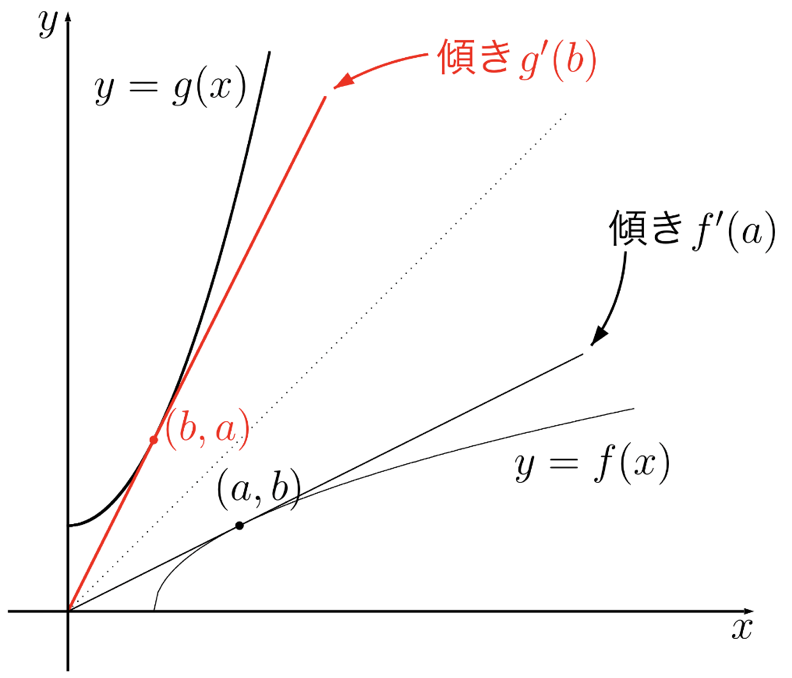
\includegraphics[width=65mm]{diff_inv.png}
 \end{center}
\end{figure}



\end{frame}



%%%%%%%%%%%%%%%%%%%%%%%%%%%%%%%%%%%%%%%%%%%%%%%%%%%%%%%%%%%%%%%%%%%%%%%%%%%%%%%%%%%%%%%
%%%%%%%%%%%%%%%%%%%%%%%%%%%%%%%%%%%%%%%%%%%%%%%%%%%%%%%%%%%%%%%%%%%%%%%%%%%%%%%%%%%%%%%


%\begin{frame}
%\frametitle{逆関数の微分}
%
%\begin{Prob}
%次の関数$f,g$は互いに逆関数の関係にあった. 
%\begin{enumerate}
%\item $f:\R \longrightarrow \R, \  x \mapsto 2x-4, \ \  g:\R \longrightarrow \R, \ y \mapsto \frac{1}{2}y+2$, 
%\item $f: \R \longrightarrow \R_+, \  x \mapsto e^x, \ \ g: \R_+ \longrightarrow \R, \ y \mapsto \log y$, 
%\item $f: \R_+ \longrightarrow \R_+,  \  x \mapsto x^2, \ \ g: \R_+ \longrightarrow \R_+,  \ y \mapsto \sqrt{y}$. 
%\end{enumerate}
%これらに関して, 逆関数の微分公式を確認せよ. 
%\end{Prob}
%
%\end{frame}



%%%%%%%%%%%%%%%%%%%%%%%%%%%%%%%%%%%%%%%%%%%%%%%%%%%%%%%%%%%%%%%%%%%%%%%%%%%%%%%%%%%%%%%
%%%%%%%%%%%%%%%%%%%%%%%%%%%%%%%%%%%%%%%%%%%%%%%%%%%%%%%%%%%%%%%%%%%%%%%%%%%%%%%%%%%%%%%


\begin{frame}
\frametitle{逆関数の微分}


関数
$$
f:\R \longrightarrow \R, \  x \mapsto 2x-4, \ \ \  g:\R \longrightarrow \R, \ y \mapsto \frac{1}{2}y+2
$$
は互いに逆写像の関係にあった. \\
\ \\

実際に導関数を計算してみると
$$
f'(x)=2, \ \ \ g'(y)= \frac{1}{2}
$$
であるから, 確かに
\begin{align*}
 \frac{1}{g'(2x-4)} = 2 = f'(x), \ \ \ \frac{1}{f'(\frac{1}{2}y+2)}=\frac{1}{2}=g'(y). 
\end{align*}



\end{frame}




%%%%%%%%%%%%%%%%%%%%%%%%%%%%%%%%%%%%%%%%%%%%%%%%%%%%%%%%%%%%%%%%%%%%%%%%%%%%%%%%%%%%%%%
%%%%%%%%%%%%%%%%%%%%%%%%%%%%%%%%%%%%%%%%%%%%%%%%%%%%%%%%%%%%%%%%%%%%%%%%%%%%%%%%%%%%%%%


\begin{frame}
\frametitle{逆関数の微分}


関数
\begin{align*}
f: \R \longrightarrow \R_+, \  x \mapsto e^x, \ \ \ 
g: \R_+ \longrightarrow \R, \ y \mapsto \log y
\end{align*}
は互いに逆写像の関係にあった. \\
\ \\

実際に導関数を計算してみると
$$
f'(x)=e^x, \ \ \ g'(y)= \frac{1}{y}
$$
であるから, 確かに
\begin{align*}
\frac{1}{g'(e^x)} = \frac{1}{\frac{1}{e^x}}=e^x, \ \ \ \frac{1}{f'(\log y)}=\frac{1}{e^{\log y}}=\frac{1}{y}=g'(y). 
\end{align*}



\end{frame}



%%%%%%%%%%%%%%%%%%%%%%%%%%%%%%%%%%%%%%%%%%%%%%%%%%%%%%%%%%%%%%%%%%%%%%%%%%%%%%%%%%%%%%%
%%%%%%%%%%%%%%%%%%%%%%%%%%%%%%%%%%%%%%%%%%%%%%%%%%%%%%%%%%%%%%%%%%%%%%%%%%%%%%%%%%%%%%%


\begin{frame}
\frametitle{逆関数の微分}


関数
\begin{align*}
f: \R_+ \longrightarrow \R_+,  \  x \mapsto x^2, \ \ \ g: \R_+ \longrightarrow \R_+,  \ y \mapsto \sqrt{y}
\end{align*}
は互いに逆写像の関係にあった. \\
\ \\

実際に導関数を計算してみると
$$
f'(x)=2x, \ \ \ g'(y)= \frac{1}{2\sqrt{y}}
$$
であるから, 確かに
\begin{align*}
 \frac{1}{g'(x^2)} = \frac{1}{\frac{1}{2\sqrt{x^2}}}=2x =f'(x), \ \ \ \frac{1}{f'(\sqrt{y})}=\frac{1}{2\sqrt{y}}=g'(y). 
\end{align*}



\end{frame}



%%%%%%%%%%%%%%%%%%%%%%%%%%%%%%%%%%%%%%%%%%%%%%%%%%%%%%%%%%%%%%%%%%%%%%%%%%%%%%%%%%%%%%%
%%%%%%%%%%%%%%%%%%%%%%%%%%%%%%%%%%%%%%%%%%%%%%%%%%%%%%%%%%%%%%%%%%%%%%%%%%%%%%%%%%%%%%%


\begin{frame}
\frametitle{逆関数の微分}

\begin{Prob}
$f(x)=\sqrt[3]{x}$の逆関数を求め, 逆関数の微分法(定理\ref{逆関数の微分定理})が成立していることを確かめよ. 
\end{Prob}

\end{frame}



%%%%%%%%%%%%%%%%%%%%%%%%%%%%%%%%%%%%%%%%%%%%%%%%%%%%%%%%%%%%%%%%%%%%%%%%%%%%%%%%%%%%%%%
%%%%%%%%%%%%%%%%%%%%%%%%%%%%%%%%%%%%%%%%%%%%%%%%%%%%%%%%%%%%%%%%%%%%%%%%%%%%%%%%%%%%%%%


\begin{frame}
\frametitle{逆関数の微分}


$f(x)=\sqrt[3]{x}$の逆関数は$g(y)=y^3$である. 導関数はそれぞれ
$$
f'(x)=\frac{1}{3 \sqrt[3]{x^2}}, \ \ \ g'(y)=3y^2
$$
であるから, 確かに
$$
\frac{1}{g'(\sqrt[3]{x})}=\frac{1}{3\sqrt[3]{x}^2}=f'(x), \ \ \ 
\frac{1}{f'(y^3)}=\frac{1}{\frac{1}{3 \sqrt[3]{(y^3)^2}}}=g'(y). 
$$

\end{frame}



%%%%%%%%%%%%%%%%%%%%%%%%%%%%%%%%%%%%%%%%%%%%%%%%%%%%%%%%%%%%%%%%%%%%%%%%%%%%%%%%%%%%%%%
%%%%%%%%%%%%%%%%%%%%%%%%%%%%%%%%%%%%%%%%%%%%%%%%%%%%%%%%%%%%%%%%%%%%%%%%%%%%%%%%%%%%%%%


%\begin{frame}
%\frametitle{逆関数の微分}
%
%
%$f_2(x)=x^2+4x-1$の逆関数は, $x^2+4x-1-y=0$を$x$について解いて
%$$
%g_2(y)=-2 \pm \sqrt{y+5}. 
%$$
%導関数はそれぞれ
%$$
%f_2'(x)=2x+4, \ \ \ g_2'(y)=\pm \frac{1}{2\sqrt{y+5}}
%$$
%であるから, 確かに
%\begin{align*}
%\frac{1}{g_2'(x^2+4x-1)} &= \frac{1}{\pm \frac{1}{2\sqrt{x^2+4x-1+5}}} =\pm 2(x+2)=\\
%\frac{1}{f_2'(-2 \pm \sqrt{y+5})} & = \frac{1}{2(-2 \pm \sqrt{y+5})+4}=g_2'(y). 
%\end{align*}
%
%\end{frame}



%%%%%%%%%%%%%%%%%%%%%%%%%%%%%%%%%%%%%%%%%%%%%%%%%%%%%%%%%%%%%%%%%%%%%%%%%%%%%%%%%%%%%%%
%%%%%%%%%%%%%%%%%%%%%%%%%%%%%%%%%%%%%%%%%%%%%%%%%%%%%%%%%%%%%%%%%%%%%%%%%%%%%%%%%%%%%%%

\section{逆三角関数}

\begin{frame}
\frametitle{三角関数}

三角関数$\sin x, \cos x, \tan x$を思い出す. 


 \begin{figure}[htbp]
 \begin{center} 
  \includegraphics[width=100mm]{trig2.png}
 \end{center}
\end{figure}


\end{frame}



%%%%%%%%%%%%%%%%%%%%%%%%%%%%%%%%%%%%%%%%%%%%%%%%%%%%%%%%%%%%%%%%%%%%%%%%%%%%%%%%%%%%%%%
%%%%%%%%%%%%%%%%%%%%%%%%%%%%%%%%%%%%%%%%%%%%%%%%%%%%%%%%%%%%%%%%%%%%%%%%%%%%%%%%%%%%%%%


\begin{frame}
\frametitle{逆三角関数}

\begin{itemize}
\item $\sin:[-\pi/2,\pi/2]\rightarrow [-1,1]$は全単射. 
この逆関数を$\arcsin x$と書く. 
$$
\arcsin: [-1,1] \longrightarrow [-\pi/2,\pi/2], \ \ \ x \mapsto \arcsin x. 
$$
\item $\cos:[0,\pi]\rightarrow [-1,1]$は全単射. 
この逆関数を$\arccos x$と書く. 
$$
\arccos: [-1,1] \longrightarrow [0,\pi], \ \ \ x \mapsto \arccos x. 
$$
\item $\tan:(-\pi/2,\pi/2)\rightarrow \R$は全単射. 
この逆関数を$\arctan x$と書く. 
$$
\arctan: \R \longrightarrow (-\pi/2,\pi/2), \ \ \ x \mapsto \arctan x. 
$$
\end{itemize}
これらは逆三角関数と呼ばれ, それぞれ$\sin^{-1}x, \cos^{-1}x,\tan^{-1}x$と書くこともある. 
($\arcsin x = \sin^{-1}x \neq \frac{1}{\sin x}$)




\end{frame}



%%%%%%%%%%%%%%%%%%%%%%%%%%%%%%%%%%%%%%%%%%%%%%%%%%%%%%%%%%%%%%%%%%%%%%%%%%%%%%%%%%%%%%%
%%%%%%%%%%%%%%%%%%%%%%%%%%%%%%%%%%%%%%%%%%%%%%%%%%%%%%%%%%%%%%%%%%%%%%%%%%%%%%%%%%%%%%%


\begin{frame}
\frametitle{逆三角関数}



 \begin{figure}[htbp]
 \begin{center} 
  \includegraphics[width=120mm]{inv_trig.png}
 \end{center}
\end{figure}


\end{frame}


%%%%%%%%%%%%%%%%%%%%%%%%%%%%%%%%%%%%%%%%%%%%%%%%%%%%%%%%%%%%%%%%%%%%%%%%%%%%%%%%%%%%%%%
%%%%%%%%%%%%%%%%%%%%%%%%%%%%%%%%%%%%%%%%%%%%%%%%%%%%%%%%%%%%%%%%%%%%%%%%%%%%%%%%%%%%%%%


\begin{frame}
\frametitle{逆三角関数}

%実際, $0 \le x \le 1$に関して, 逆関数は$\arcsin x$と$\arccos x$は半径$\frac{1}{2}$の円の弧(arc)の一部の長さを表している. 
実際, $0 \le x \le 1$に関して, $\arcsin x$と$\arccos x$は半径$1$の円の弧(arc)の一部の長さを表している. 

 \begin{figure}[htbp]
 \begin{center} 
  \includegraphics[width=38mm]{arc2.png}
 \end{center}
\end{figure}
\vspace{-3mm}

これより, 例えば
$$
\arcsin x + \arccos x = \frac{\pi}{2}
$$
が視覚的に理解できる. ($-1\le x \le 1$で成立.)

\end{frame}


%%%%%%%%%%%%%%%%%%%%%%%%%%%%%%%%%%%%%%%%%%%%%%%%%%%%%%%%%%%%%%%%%%%%%%%%%%%%%%%%%%%%%%%
%%%%%%%%%%%%%%%%%%%%%%%%%%%%%%%%%%%%%%%%%%%%%%%%%%%%%%%%%%%%%%%%%%%%%%%%%%%%%%%%%%%%%%%


\begin{frame}
\frametitle{逆三角関数}



\begin{Prob}
次の値を求めよ. 
\begin{enumerate}
\item $\arcsin \frac{1}{\sqrt{2}}$,  %\pi/4
\item $\arcsin 1$, %\pi/2
\item $\arccos \frac{1}{2}$, %\pi/3 
\item $\arctan \frac{1}{\sqrt{3}}$ % \pi/6
\end{enumerate}
\end{Prob}

\end{frame}



%%%%%%%%%%%%%%%%%%%%%%%%%%%%%%%%%%%%%%%%%%%%%%%%%%%%%%%%%%%%%%%%%%%%%%%%%%%%%%%%%%%%%%%
%%%%%%%%%%%%%%%%%%%%%%%%%%%%%%%%%%%%%%%%%%%%%%%%%%%%%%%%%%%%%%%%%%%%%%%%%%%%%%%%%%%%%%%


\section{逆三角関数の微分}

\begin{frame}
\frametitle{逆三角関数}

\begin{Thm}
$$
(\arcsin x)'=\frac{1}{\sqrt{1-x^2}}
$$
\end{Thm}

$f(x)=\arcsin x$の逆関数は$g(y)=\sin y$であるから
\begin{align*}
f'(x)=\frac{1}{g'(y)}=\frac{1}{\cos y}=\frac{1}{\sqrt{1-x^2}}. 
\end{align*}
ただし最後に
$$
\cos y = \sqrt{1-\sin^2 y}=\sqrt{1-x^2}
$$
を用いた. 


\end{frame}



%%%%%%%%%%%%%%%%%%%%%%%%%%%%%%%%%%%%%%%%%%%%%%%%%%%%%%%%%%%%%%%%%%%%%%%%%%%%%%%%%%%%%%%
%%%%%%%%%%%%%%%%%%%%%%%%%%%%%%%%%%%%%%%%%%%%%%%%%%%%%%%%%%%%%%%%%%%%%%%%%%%%%%%%%%%%%%%


\begin{frame}
\frametitle{逆三角関数}

\begin{Thm}
$$
(\arccos x)'= - \frac{1}{\sqrt{1-x^2}}
$$
\end{Thm}

$f(x)=\arccos x$の逆関数は$g(y)=\cos y$であるから
\begin{align*}
f'(x)=\frac{1}{g'(y)}=\frac{1}{- \sin y}=-\frac{1}{\sqrt{1-x^2}}. 
\end{align*}
\end{frame}


%%%%%%%%%%%%%%%%%%%%%%%%%%%%%%%%%%%%%%%%%%%%%%%%%%%%%%%%%%%%%%%%%%%%%%%%%%%%%%%%%%%%%%%
%%%%%%%%%%%%%%%%%%%%%%%%%%%%%%%%%%%%%%%%%%%%%%%%%%%%%%%%%%%%%%%%%%%%%%%%%%%%%%%%%%%%%%%


\begin{frame}
\frametitle{逆三角関数}

\begin{Thm}
$$
(\arctan x)'= \frac{1}{1+x^2}
$$
\end{Thm}

$f(x)=\arctan x$の逆関数は$g(y)=\tan y$であるから
\begin{align*}
f'(x)=\frac{1}{g'(y)}=\frac{1}{\frac{1}{\cos^2 y}}=\cos^2 y = \frac{1}{1+x^2}.  
\end{align*}
ただし最後に
$$
\cos^2 y \cdot (1+\tan^2 y)=\cos^2 y + \sin^2 y = 1
$$
を用いた. 

\end{frame}


%%%%%%%%%%%%%%%%%%%%%%%%%%%%%%%%%%%%%%%%%%%%%%%%%%%%%%%%%%%%%%%%%%%%%%%%%%%%%%%%%%%%%%%
%%%%%%%%%%%%%%%%%%%%%%%%%%%%%%%%%%%%%%%%%%%%%%%%%%%%%%%%%%%%%%%%%%%%%%%%%%%%%%%%%%%%%%%


\begin{frame}
\frametitle{逆三角関数}

\begin{Prob}
次の関数の導関数を求めよ. 
\begin{enumerate}
\item $\arcsin 3x^2$, 
\item $\arctan (x^3+1)$
\end{enumerate}
\end{Prob}

\end{frame}

%%%%%%%%%%%%%%%%%%%%%%%%%%%%%%%%%%%%%%%%%%%%%%%%%%%%%%%%%%%%%%%%%%%%%%%%%%%%%%%%%%%%%%%
%%%%%%%%%%%%%%%%%%%%%%%%%%%%%%%%%%%%%%%%%%%%%%%%%%%%%%%%%%%%%%%%%%%%%%%%%%%%%%%%%%%%%%%





%%%%%%%%%%%%%%%%%%%%%%%%%%%%%%%%%%%%%%%%%%%%%%%%%%%%%%%%%%%%%%%%%%%%%%%%%%%%%%%%%%%%%%%
%%%%%%%%%%%%%%%%%%%%%%%%%%%%%%%%%%%%%%%%%%%%%%%%%%%%%%%%%%%%%%%%%%%%%%%%%%%%%%%%%%%%%%%




\section{今日のまとめ}
\begin{frame}
\frametitle{まとめ}   

\begin{enumerate}
\item 逆写像, 逆関数, 逆関数の微分
\item 逆三角関数, 逆三角関数の微分
\end{enumerate} 




\end{frame}


\end{document}
\section{講義概要}


\begin{frame}
\frametitle{今日の内容}


微分法の応用に関して解説する. 
\begin{enumerate}
\item 接線と法線の方程式
\item 極値問題, 凹凸, $2$次導関数
\item ロピタルの定理
\end{enumerate} 



\end{frame}




%%%%%%%%%%%%%%%%%%%%%%%%%%%%%%%%%%%%%%%%%%%%%%%%%%%%%%%%%%%%%%%%%%%%%%%%%%%%%%%%%%%%%%%
%%%%%%%%%%%%%%%%%%%%%%%%%%%%%%%%%%%%%%%%%%%%%%%%%%%%%%%%%%%%%%%%%%%%%%%%%%%%%%%%%%%%%%%


%%%%%%%%%%%%%%%%%%%%%%%%%%%%%%%%%%%%%%%%%%%%%%%%%%%%%%%%%%%%%%%%%%%%%%%%%%%%%%%%%%%%%%%
%%%%%%%%%%%%%%%%%%%%%%%%%%%%%%%%%%%%%%%%%%%%%%%%%%%%%%%%%%%%%%%%%%%%%%%%%%%%%%%%%%%%%%%



\section{接線と法線}


\begin{frame}
\frametitle{接線と法線}

\begin{itemize}
\item 関数$f(x)$が$a$で微分可能とは, 点$(a,f(a))$の近傍で$f(x)$のグラフが直線で近似可能であること. 
その直線の傾きは微分係数$f'(a)$で与えられる.  
\item 関数のグラフが直線であれば関数の増加・減少はその傾きの正負で簡単に判定できる.  
そのため, 関数を微分することにより, その関数がどの範囲で増加・減少しているかを解析することが可能になる. 
\end{itemize}

 \begin{figure}[htbp]
 \begin{center} 
  \includegraphics[width=80mm]{calculus7/differentiable2.png}
 \end{center}
\end{figure}




\end{frame}



%%%%%%%%%%%%%%%%%%%%%%%%%%%%%%%%%%%%%%%%%%%%%%%%%%%%%%%%%%%%%%%%%%%%%%%%%%%%%%%%%%%%%%%
%%%%%%%%%%%%%%%%%%%%%%%%%%%%%%%%%%%%%%%%%%%%%%%%%%%%%%%%%%%%%%%%%%%%%%%%%%%%%%%%%%%%%%%





\begin{frame}
\frametitle{接線}

\vspace{-2mm}

\begin{Def}
関数$f(x)$が$a$で微分可能であるとする. 
点$(a,f(a))$を通る傾き$f'(a)$の直線を, $y=f(x)$のグラフの$(a,f(a))$における\underline{接線}という. 
具体的に式で書くと
$$
y-f(a)=f'(a)(x-a). 
$$
\end{Def}
式を整理して
$$
y=f'(a)x + f(a) -f'(a)a
$$
と書くこともできる. 
\vspace{-2mm}

 \begin{figure}[htbp]
 \begin{center} 
  \includegraphics[width=70mm]{calculus7/tangent.png}
 \end{center}
\end{figure}


\end{frame}



%%%%%%%%%%%%%%%%%%%%%%%%%%%%%%%%%%%%%%%%%%%%%%%%%%%%%%%%%%%%%%%%%%%%%%%%%%%%%%%%%%%%%%%
%%%%%%%%%%%%%%%%%%%%%%%%%%%%%%%%%%%%%%%%%%%%%%%%%%%%%%%%%%%%%%%%%%%%%%%%%%%%%%%%%%%%%%%





\begin{frame}
\frametitle{接線}


関数$f(x)=x^2-x-3$のグラフの$(2,f(2))$における接線を求める. \\
\ \\

導関数は$f'(x)=2x-1$である. 
$f(2)=-1$, $f'(2)=3$より, 接線の方程式は
$$
y-(-1)=3(x-2), 
$$
つまり
$$
y=3x-7. 
$$




\end{frame}

%%%%%%%%%%%%%%%%%%%%%%%%%%%%%%%%%%%%%%%%%%%%%%%%%%%%%%%%%%%%%%%%%%%%%%%%%%%%%%%%%%%%%%%
%%%%%%%%%%%%%%%%%%%%%%%%%%%%%%%%%%%%%%%%%%%%%%%%%%%%%%%%%%%%%%%%%%%%%%%%%%%%%%%%%%%%%%%





\begin{frame}
\frametitle{法線}


\begin{Def}
関数$f(x)$が$a$で微分可能であるとする. 
点$(a,f(a))$において, $y=f(x)$のグラフの接線と直交する直線を\underline{法線}という. 
具体的に式で書くと
$$
y-f(a)=-\frac{1}{f'(a)}(x-a). 
$$
\end{Def}
\begin{itemize}
\item 式を整理して
$$
y=-\frac{1}{f'(a)}x + f(a) +\frac{a}{f'(a)}
$$
と書くこともできる.  
\item 傾きが$s$と$t$の直線が直交する条件は$st=-1$である. (非自明)
\end{itemize}

\end{frame}




%%%%%%%%%%%%%%%%%%%%%%%%%%%%%%%%%%%%%%%%%%%%%%%%%%%%%%%%%%%%%%%%%%%%%%%%%%%%%%%%%%%%%%%
%%%%%%%%%%%%%%%%%%%%%%%%%%%%%%%%%%%%%%%%%%%%%%%%%%%%%%%%%%%%%%%%%%%%%%%%%%%%%%%%%%%%%%%





\begin{frame}
\frametitle{法線}


関数$f(x)=x^2-x-3$のグラフの$(2,f(2))$における法線を求める. \\
\ \\

導関数は$f'(x)=2x-1$である. 
$f(2)=-1$, $f'(2)=3$より, 法線の方程式は
$$
y-(-1)=-\frac{1}{3}(x-2), 
$$
つまり
$$
y=-\frac{1}{3}x-\frac{1}{3}.  
$$




\end{frame}




%%%%%%%%%%%%%%%%%%%%%%%%%%%%%%%%%%%%%%%%%%%%%%%%%%%%%%%%%%%%%%%%%%%%%%%%%%%%%%%%%%%%%%%
%%%%%%%%%%%%%%%%%%%%%%%%%%%%%%%%%%%%%%%%%%%%%%%%%%%%%%%%%%%%%%%%%%%%%%%%%%%%%%%%%%%%%%%

\section{極値問題}



\begin{frame}
\frametitle{単調増加, 単調減少}


\begin{Def}
\begin{itemize}
\item 関数$f(x)$は
$$
x_1 < x_2 \ \Rightarrow \ f(x_1)  \le f(x_2)
$$
を満たすとき, \underline{単調増加}と呼ばれ, 
$$
x_1 < x_2 \ \Rightarrow \ f(x_1)  \ge f(x_2)
$$
を満たすとき, \underline{単調減少}と呼ばれる. 
\item $\le$を$<$に置き換えた条件を満たすとき, \underline{狭義単調増加}と呼ばれ, 
$\ge$を$>$に置き換えた条件を満たすとき, \underline{狭義単調減少}と呼ばれる. 
\end{itemize}
\end{Def}




\end{frame}


%%%%%%%%%%%%%%%%%%%%%%%%%%%%%%%%%%%%%%%%%%%%%%%%%%%%%%%%%%%%%%%%%%%%%%%%%%%%%%%%%%%%%%%
%%%%%%%%%%%%%%%%%%%%%%%%%%%%%%%%%%%%%%%%%%%%%%%%%%%%%%%%%%%%%%%%%%%%%%%%%%%%%%%%%%%%%%%



\begin{frame}
\frametitle{単調増加, 単調減少}


関数の増減と微分に関して, 次の関係は基本的である. 

\begin{Thm}
関数$f(x)$が微分可能であるとする. 
\begin{itemize}
\item $f'(x)\ge0$ならば$f(x)$は単調増加. 
\item $f'(x)>0$ならば$f(x)$は狭義単調増加. 
\item $f'(x)\le0$ならば$f(x)$は単調減少. 
\item $f'(x)<0$ならば$f(x)$は狭義単調減少. 
\item $f'(x)=0$ならば$f(x)$は定数. 
\end{itemize}
\end{Thm}
微分係数が接線の傾きを与えていることを思い出せば, 直感的に理解しやすい. 


\end{frame}


%%%%%%%%%%%%%%%%%%%%%%%%%%%%%%%%%%%%%%%%%%%%%%%%%%%%%%%%%%%%%%%%%%%%%%%%%%%%%%%%%%%%%%%
%%%%%%%%%%%%%%%%%%%%%%%%%%%%%%%%%%%%%%%%%%%%%%%%%%%%%%%%%%%%%%%%%%%%%%%%%%%%%%%%%%%%%%%



\begin{frame}
\frametitle{極大・極小}
\vspace{-2.5mm}

\begin{Def}
関数$f(x)$は$a$の近傍($a$を含む小さな開区間)において
\begin{itemize} 
\item $x<a$で単調増加,  $x>a$で単調減少となるとき, $f(x)$は$a$で\underline{極大}であるといい, $f(a)$を\underline{極大値}という.
\item  $x<a$で単調減少,  $x>a$で単調増加となるとき, $f(x)$は$a$で\underline{極小}であるといい, $f(a)$を\underline{極小値}という.
\end{itemize}
\underline{極値}: 極大値と極小値, \underline{極値問題}: 極値を求める問題. 
\end{Def}

関数の最大値と最小値はそれぞれ極大値と極小値. 

\vspace{-1mm}

 \begin{figure}[htbp]
 \begin{center} 
  \includegraphics[width=65mm]{calculus7/local_maxmin.png}
 \end{center}
\end{figure}

\end{frame}


%%%%%%%%%%%%%%%%%%%%%%%%%%%%%%%%%%%%%%%%%%%%%%%%%%%%%%%%%%%%%%%%%%%%%%%%%%%%%%%%%%%%%%%
%%%%%%%%%%%%%%%%%%%%%%%%%%%%%%%%%%%%%%%%%%%%%%%%%%%%%%%%%%%%%%%%%%%%%%%%%%%%%%%%%%%%%%%



\begin{frame}
\frametitle{ワイエルシュトラスの定理}



連続関数の最大値と最小値に関しては次の定理が知られている. 

\begin{Thm}[ワイエルシュトラスの定理] \label{Weierstrass}
関数$f(x)$が$[a,b]$で連続であるとき, $c,d\in [a,b]$が存在して, 任意の$x \in [a,b]$に対して
$$
f(x) \le f(c), \ \ \ f(d) \le f(x). 
$$
つまり, $f(x)$は$[a,b]$において$c$で最大値$f(c)$, $d$で最小値$f(d)$をとる. 
\end{Thm}
\begin{itemize}
\item 定理\ref{Weierstrass}は関数が具体的にどこで最大値と最小値をとるのかについてまでは教えてくれない. 
\item 連続性を仮定するのは何故であろうか? 
\end{itemize}
\end{frame}

%%%%%%%%%%%%%%%%%%%%%%%%%%%%%%%%%%%%%%%%%%%%%%%%%%%%%%%%%%%%%%%%%%%%%%%%%%%%%%%%%%%%%%%
%%%%%%%%%%%%%%%%%%%%%%%%%%%%%%%%%%%%%%%%%%%%%%%%%%%%%%%%%%%%%%%%%%%%%%%%%%%%%%%%%%%%%%%



\begin{frame}
\frametitle{極大・極小}


\begin{Def}
関数$f(x)$が微分可能であるとき, $f'(a)=0$なる$a$を$f(x)$の\underline{停留点}という. 
\end{Def}

\begin{itemize}
\item $f(x)$が$a$で極大・極小であれば$a$は$f(x)$の停留点である. 
\begin{itemize}
\item 極大: $f'(x)$の符号が$a$で正から負に変化
\item 極小: $f'(x)$の符号が$a$で負から正に変化
\end{itemize}
\item 停留点は極大・極小とは限らない. 実際, $f(x)=x^3$の停留点$a=0$は極大でも極小でもない. 
\item 極値問題では, 導関数を計算して停留点を求め, それが極大・極小を与えているか確認する, という方法を採る. 
\end{itemize}
\end{frame}



%%%%%%%%%%%%%%%%%%%%%%%%%%%%%%%%%%%%%%%%%%%%%%%%%%%%%%%%%%%%%%%%%%%%%%%%%%%%%%%%%%%%%%%
%%%%%%%%%%%%%%%%%%%%%%%%%%%%%%%%%%%%%%%%%%%%%%%%%%%%%%%%%%%%%%%%%%%%%%%%%%%%%%%%%%%%%%%



\begin{frame}
\frametitle{増減表}

増減表: 関数の増減と極値に関して纏めた表.\\
\ \\

$f(x)=2x^2+8x+13$に関して, 
$$
f'(x)=4x+8=4(x+2) \vspace{-4.5mm}
$$
\begin{itemize}
\item $f'(x)<0 \ \Leftrightarrow \ x<-2$, 
\item $f'(x)=0 \ \Leftrightarrow \ x=-2$, 
\item $f'(x)>0 \ \Leftrightarrow \ x>-2$, 
\end{itemize}

\begin{table}[htb]
\begin{center}
\begin{tabular}{c|c|c|c}
$x$ & $\dots$ & $-2$ & $\dots$ \\ \hline 
$f'(x)$   & $-$ & 0  & $+$   \\ \hline 
$f(x)$   & $\searrow$ & $5$ &  $\nearrow$  
  \end{tabular}
  \end{center}
\end{table}

\end{frame}




%%%%%%%%%%%%%%%%%%%%%%%%%%%%%%%%%%%%%%%%%%%%%%%%%%%%%%%%%%%%%%%%%%%%%%%%%%%%%%%%%%%%%%%
%%%%%%%%%%%%%%%%%%%%%%%%%%%%%%%%%%%%%%%%%%%%%%%%%%%%%%%%%%%%%%%%%%%%%%%%%%%%%%%%%%%%%%%



\begin{frame}
\frametitle{増減表}

$f(x)=x^3+3x^2-9x+6$に関して, 
$$
f'(x)=3x^2+6x-9=3(x+3)(x-1) \vspace{-4.5mm}
$$
\begin{itemize}
\item $f'(x)<0 \ \Leftrightarrow \ -3<x<1$, 
\item $f'(x)=0 \ \Leftrightarrow \ x=-3,1$, 
\item $f'(x)>0 \ \Leftrightarrow \ x<-3 \ \text{or} \ x>1$, 
\end{itemize}

\begin{table}[htb]
\begin{center}
\begin{tabular}{c|c|c|c|c|c}
$x$ & $\dots$ & $-3$ & $\dots$ & 1 & \dots \\ \hline 
$f'(x)$   & $+$ & $0$  & $-$  & $0$ & $+$   \\ \hline 
$f(x)$   & $\nearrow$  & $33$ & $\searrow$  & $1$ &  $\nearrow$  
  \end{tabular}
  \end{center}
\end{table}

\end{frame}


%%%%%%%%%%%%%%%%%%%%%%%%%%%%%%%%%%%%%%%%%%%%%%%%%%%%%%%%%%%%%%%%%%%%%%%%%%%%%%%%%%%%%%%
%%%%%%%%%%%%%%%%%%%%%%%%%%%%%%%%%%%%%%%%%%%%%%%%%%%%%%%%%%%%%%%%%%%%%%%%%%%%%%%%%%%%%%%



\begin{frame}
\frametitle{関数の凹凸}


\begin{Def}
開区間$I$において, 関数$f(x)$が
\begin{itemize}
\item \underline{下に凸}: 任意の$x_1,x_2 \in I$と$0 \le \lambda \le 1$に対して
$$
\lambda f(x_1)+(1-\lambda)f(x_2) \ge f(\lambda x_1+(1-\lambda)x_2). 
$$
\item \underline{上に凸}: 任意の$x_1,x_2 \in I$と$0 \le \lambda \le 1$に対して
$$
\lambda f(x_1)+(1-\lambda)f(x_2) \le f(\lambda x_1+(1-\lambda)x_2). 
$$
\end{itemize}
\end{Def}

点$p,q$に対して, $\lambda p+(1-\lambda)q$は点$p,q$間を$\lambda:(1-\lambda)$に内分する点. 


\end{frame}


%%%%%%%%%%%%%%%%%%%%%%%%%%%%%%%%%%%%%%%%%%%%%%%%%%%%%%%%%%%%%%%%%%%%%%%%%%%%%%%%%%%%%%%
%%%%%%%%%%%%%%%%%%%%%%%%%%%%%%%%%%%%%%%%%%%%%%%%%%%%%%%%%%%%%%%%%%%%%%%%%%%%%%%%%%%%%%%



\begin{frame}
\frametitle{関数の凹凸}


関数の凹凸は視覚的に理解するのが良い. 
グラフ上の2点を結んだ線分が常にグラフの上側(下側)にあるような関数が下に凸(上に凸).


 \begin{figure}[htbp]
 \begin{center} 
  \includegraphics[width=100mm]{calculus7/convex.png}
 \end{center}
\end{figure}


\end{frame}



%%%%%%%%%%%%%%%%%%%%%%%%%%%%%%%%%%%%%%%%%%%%%%%%%%%%%%%%%%%%%%%%%%%%%%%%%%%%%%%%%%%%%%%
%%%%%%%%%%%%%%%%%%%%%%%%%%%%%%%%%%%%%%%%%%%%%%%%%%%%%%%%%%%%%%%%%%%%%%%%%%%%%%%%%%%%%%%



\begin{frame}
\frametitle{関数の凹凸}


その点の左右で上に凸と下に凸とが切り替わるような点を\underline{変曲点}という.


 \begin{figure}[htbp]
 \begin{center} 
  \includegraphics[width=85mm]{calculus7/inflection.png}
 \end{center}
\end{figure}


\end{frame}


%%%%%%%%%%%%%%%%%%%%%%%%%%%%%%%%%%%%%%%%%%%%%%%%%%%%%%%%%%%%%%%%%%%%%%%%%%%%%%%%%%%%%%%
%%%%%%%%%%%%%%%%%%%%%%%%%%%%%%%%%%%%%%%%%%%%%%%%%%%%%%%%%%%%%%%%%%%%%%%%%%%%%%%%%%%%%%%



\begin{frame}
\frametitle{2次導関数}


関数の増減は微分することで判定ができた. 
次に関数の凹凸は$2$回微分することにより判定できることを説明する. 

\begin{Def}
関数$f(x)$の導関数$f'(x)$も微分可能であるとき, $f(x)$は\underline{$2$回微分可能}であるという. 
$f'(x)$の導関数を$f''(x)$と書き, $f(x)$の\underline{$2$次導関数}と呼ぶ. 
\end{Def}

$f(x)$が位置を表すとき, 
\begin{itemize}
\item $f'(x)$は速度(=位置の変化率), 
\item $f''(x)$は加速度(=速度の変化率) 
\end{itemize}
を表す.
\end{frame}


%%%%%%%%%%%%%%%%%%%%%%%%%%%%%%%%%%%%%%%%%%%%%%%%%%%%%%%%%%%%%%%%%%%%%%%%%%%%%%%%%%%%%%%
%%%%%%%%%%%%%%%%%%%%%%%%%%%%%%%%%%%%%%%%%%%%%%%%%%%%%%%%%%%%%%%%%%%%%%%%%%%%%%%%%%%%%%%



\begin{frame}
\frametitle{2次導関数}
\vspace{-2mm}

\begin{Thm}
$f(x)$は$2$回微分可能とする. 
\begin{itemize}
\item $f''(x)>0$ならば$f(x)$は下に凸. 
\item $f''(x)<0$ならば$f(x)$は上に凸.
\item 変曲点$a$は$2$階微分の符号が変化する点. 特に$f''(a)=0$
\end{itemize}
\end{Thm}
$f''(x)>0$は接線の傾きが増加すること, $f''(x)<0$は接線の傾きが減少することを意味する. 

\vspace{-1mm}

 \begin{figure}[htbp]
 \begin{center} 
  \includegraphics[width=85mm]{calculus7/inflection2.png}
 \end{center}
\end{figure}

\end{frame}


%%%%%%%%%%%%%%%%%%%%%%%%%%%%%%%%%%%%%%%%%%%%%%%%%%%%%%%%%%%%%%%%%%%%%%%%%%%%%%%%%%%%%%%
%%%%%%%%%%%%%%%%%%%%%%%%%%%%%%%%%%%%%%%%%%%%%%%%%%%%%%%%%%%%%%%%%%%%%%%%%%%%%%%%%%%%%%%



\begin{frame}
\frametitle{正規分布の変曲点}
%https://manabitimes.jp/math/1214

正数$a>0$に関して, $f(x)=e^{-ax^2}$の変曲点を求める. 
\begin{align*}
f'(x) & = -2axe^{-ax^2} \\
f''(x) & = -2ae^{-ax^2} + (-2ax)^2e^{-ax^2} \\
&= 2ae^{-ax^2} (2ax^2-1)
\end{align*}
これより$x=\pm \frac{1}{\sqrt{2a}}$が変曲点. \\
\ \\

特に$a=\frac{1}{2\sigma^2}$とすると, $x=\pm \sigma$が変曲点. 

\end{frame}




%%%%%%%%%%%%%%%%%%%%%%%%%%%%%%%%%%%%%%%%%%%%%%%%%%%%%%%%%%%%%%%%%%%%%%%%%%%%%%%%%%%%%%%
%%%%%%%%%%%%%%%%%%%%%%%%%%%%%%%%%%%%%%%%%%%%%%%%%%%%%%%%%%%%%%%%%%%%%%%%%%%%%%%%%%%%%%%



\begin{frame}
\frametitle{正規分布の変曲点 (発展)}

\begin{Thm}
正規分布の確率密度関数$f(x)=\frac{1}{\sqrt{2 \pi \sigma}}e^{-\frac{(x-\mu)^2}{2\sigma^2}}$の変曲点は$x=\mu \pm \sigma$. 
\end{Thm}
$\sigma$は正規分布の標準偏差と呼ばれる. 


 \begin{figure}[htbp]
 \begin{center} 
  \includegraphics[width=65mm]{calculus7/normal_sigma.png}
 \end{center}
\end{figure}

\end{frame}

%%%%%%%%%%%%%%%%%%%%%%%%%%%%%%%%%%%%%%%%%%%%%%%%%%%%%%%%%%%%%%%%%%%%%%%%%%%%%%%%%%%%%%%
%%%%%%%%%%%%%%%%%%%%%%%%%%%%%%%%%%%%%%%%%%%%%%%%%%%%%%%%%%%%%%%%%%%%%%%%%%%%%%%%%%%%%%%



\begin{frame}
\frametitle{2次導関数}

停留点は極値とは限らなかったが, $2$次導関数を使うことで, 極大・極小についての判定が可能となる. 


\begin{Thm} \label{2回微分と極値}
$f(x)$は$2$回微分可能とする. 
\begin{itemize}
\item $f'(a)=0$かつ$f''(a)>0$ならば$f(x)$は$a$において極小. 
\item $f'(a)=0$かつ$f''(a)<0$ならば$f(x)$は$a$において極大.  
\end{itemize}
\end{Thm}

\begin{itemize}
\item $f'(a)=f''(a)=0$である場合には, 定理\ref{2回微分と極値}からは何も分からない. 
\item 実際, $f(x)=x^3$に関して, $f'(0)=f''(0)=0$であり, $f(x)$は原点$0$において極値をとらない.  
\end{itemize}
\end{frame}


%%%%%%%%%%%%%%%%%%%%%%%%%%%%%%%%%%%%%%%%%%%%%%%%%%%%%%%%%%%%%%%%%%%%%%%%%%%%%%%%%%%%%%%
%%%%%%%%%%%%%%%%%%%%%%%%%%%%%%%%%%%%%%%%%%%%%%%%%%%%%%%%%%%%%%%%%%%%%%%%%%%%%%%%%%%%%%%



\begin{frame}
\frametitle{増減凹凸表}

増減凹凸表: 関数の増減, 凹凸, 極値に関して纏めた表.\\
\ \\

$f(x)=x^3+3x^2-9x+6$に関して, 
\begin{align*}
f'(x) &= 3x^2+6x-9=3(x+3)(x-1) \\
f''(x) &= 6x+6=6(x+1)\vspace{-4.5mm}
\end{align*}

これより$f(x)$の増減凹凸表は次で与えられる. 

\begin{table}[htb]
\begin{center}
\begin{tabular}{c|c|c|c|c|c|c|c}
$x$ & $\dots$ & $-3$ & $\dots$ & $-1$ & \dots & 1 & \dots \\ \hline 
$f'(x)$   & $+$ & $0$  & $-$ & $-$ & $-$  & $0$ & $+$   \\ \hline 
$f ''(x)$   & $-$ & $-$  & $-$ & $0$ &  $+$ & $+$  & $+$   \\ \hline 
$f(x)$   & \nel  & $33$ & \sel & $17$ & \ser &  $1$  & \ner   
  \end{tabular}
  \end{center}
\end{table}

\end{frame}



%%%%%%%%%%%%%%%%%%%%%%%%%%%%%%%%%%%%%%%%%%%%%%%%%%%%%%%%%%%%%%%%%%%%%%%%%%%%%%%%%%%%%%%
%%%%%%%%%%%%%%%%%%%%%%%%%%%%%%%%%%%%%%%%%%%%%%%%%%%%%%%%%%%%%%%%%%%%%%%%%%%%%%%%%%%%%%%



\begin{frame}
\frametitle{増減凹凸表}

\begin{Prob}
$x>0$に対して定義される関数$f(x)=x\log x$の増減凹凸表を作り, $f(x)$のグラフを描け. 
\end{Prob}

\vspace{5.5cm}

\end{frame}

%%%%%%%%%%%%%%%%%%%%%%%%%%%%%%%%%%%%%%%%%%%%%%%%%%%%%%%%%%%%%%%%%%%%%%%%%%%%%%%%%%%%%%%
%%%%%%%%%%%%%%%%%%%%%%%%%%%%%%%%%%%%%%%%%%%%%%%%%%%%%%%%%%%%%%%%%%%%%%%%%%%%%%%%%%%%%%%


\begin{frame}
\frametitle{最適化問題}   

\begin{itemize}
\item 等周問題: 周の長さが$l$の長方形の中で面積を最大にするものは? 
\item 面積$A(x)=x(l/2-x)$
$$
A'(x)=\frac{l}{2}-2x, \ \ \ A''(x)=-2. 
$$
\end{itemize}

 \begin{figure}[htbp]
 \begin{center} 
  \includegraphics[width=90mm]{calculus7/LecArea.png}
 \end{center}
\end{figure}

\end{frame}




%%%%%%%%%%%%%%%%%%%%%%%%%%%%%%%%%%%%%%%%%%%%%%%%%%%%%%%%%%%%%%%%%%%%%%%%%%%%%%%%%%%%%%%
%%%%%%%%%%%%%%%%%%%%%%%%%%%%%%%%%%%%%%%%%%%%%%%%%%%%%%%%%%%%%%%%%%%%%%%%%%%%%%%%%%%%%%%

%%%%%%%%%%%%%%%%%%%%%%%%%%%%%%%%%%%%%%%%%%%%%%%%%%%%%%%%%%%%%%%%%%%%%%%%%%%%%%%%%%%%%%%
%%%%%%%%%%%%%%%%%%%%%%%%%%%%%%%%%%%%%%%%%%%%%%%%%%%%%%%%%%%%%%%%%%%%%%%%%%%%%%%%%%%%%%%





%%%%%%%%%%%%%%%%%%%%%%%%%%%%%%%%%%%%%%%%%%%%%%%%%%%%%%%%%%%%%%%%%%%%%%%%%%%%%%%%%%%%%%%
%%%%%%%%%%%%%%%%%%%%%%%%%%%%%%%%%%%%%%%%%%%%%%%%%%%%%%%%%%%%%%%%%%%%%%%%%%%%%%%%%%%%%%%




\section{今日のまとめ}
\begin{frame}
\frametitle{まとめ}   


\begin{enumerate}
\item 接線と法線の方程式、
\item 極値問題, 凹凸, 2次導関数
\end{enumerate} 

\end{frame}

\section{講義概要}


\begin{frame}
\frametitle{今日の内容}



\begin{enumerate}
\item ロルの定理, 平均値の定理, コーシーの平均値の定理, 
\item 高次導関数, テイラーの定理, 有限テイラー展開
\end{enumerate} 



\end{frame}




%%%%%%%%%%%%%%%%%%%%%%%%%%%%%%%%%%%%%%%%%%%%%%%%%%%%%%%%%%%%%%%%%%%%%%%%%%%%%%%%%%%%%%%
%%%%%%%%%%%%%%%%%%%%%%%%%%%%%%%%%%%%%%%%%%%%%%%%%%%%%%%%%%%%%%%%%%%%%%%%%%%%%%%%%%%%%%%


%%%%%%%%%%%%%%%%%%%%%%%%%%%%%%%%%%%%%%%%%%%%%%%%%%%%%%%%%%%%%%%%%%%%%%%%%%%%%%%%%%%%%%%
%%%%%%%%%%%%%%%%%%%%%%%%%%%%%%%%%%%%%%%%%%%%%%%%%%%%%%%%%%%%%%%%%%%%%%%%%%%%%%%%%%%%%%%



\section{ロルの定理}


\begin{frame}
\frametitle{ロルの定理}


\begin{Thm}[ロルの定理]
微分可能な関数$f(x)$の定義域に$[a,b]$が含まれ, $f(a)=f(b)$が成り立つならば, 
$f'(c)=0$なる$c \in (a,b)$が存在する. 
\end{Thm}

$f(x)$が定数関数であれば明らか. 
そうでない場合には, ワイエルシュトラスの定理より, ある$c \in (a,b)$において最大値または最小値をとる. 
$c$において$f(x)$が極値をとるので, $f'(c)=0$. 

 \begin{figure}[htbp]
 \begin{center} 
  \includegraphics[width=50mm]{calculus8/Roll.png}
 \end{center}
\end{figure}

\end{frame}



%%%%%%%%%%%%%%%%%%%%%%%%%%%%%%%%%%%%%%%%%%%%%%%%%%%%%%%%%%%%%%%%%%%%%%%%%%%%%%%%%%%%%%%
%%%%%%%%%%%%%%%%%%%%%%%%%%%%%%%%%%%%%%%%%%%%%%%%%%%%%%%%%%%%%%%%%%%%%%%%%%%%%%%%%%%%%%%




\begin{frame}
\frametitle{平均値の定理}

ロルの定理を斜めにずらしたものが平均値の定理である. 

\begin{Thm}[平均値の定理]
微分可能な関数$f(x)$の定義域に$[a,b]$が含まれるとき,
$$
f'(c)=\frac{f(b)-f(a)}{b-a}
$$
を満たす$c \in (a,b)$が存在する. 
\end{Thm}

 \begin{figure}[htbp]
 \begin{center} 
  \includegraphics[width=50mm]{calculus8/Mean.png}
 \end{center}
\end{figure}

\end{frame}




%%%%%%%%%%%%%%%%%%%%%%%%%%%%%%%%%%%%%%%%%%%%%%%%%%%%%%%%%%%%%%%%%%%%%%%%%%%%%%%%%%%%%%%
%%%%%%%%%%%%%%%%%%%%%%%%%%%%%%%%%%%%%%%%%%%%%%%%%%%%%%%%%%%%%%%%%%%%%%%%%%%%%%%%%%%%%%%




\begin{frame}
\frametitle{平均値の定理の証明}


関数 
$$
g(x)=f(x)-\frac{f(b)-f(a)}{b-a}x
$$
は$g(a)=g(b)$を満たすので, ロルの定理より$g'(c)=0$なる$c \in (a,b)$が存在する. 
$$
0=g'(c)=f'(c)-\frac{f(b)-f(a)}{b-a}
$$
なので, 平均値の定理が示された. \\
\ \\

端点で関数の値が等しくなるように一次関数を引くことで, ロルの定理に帰着させている. 

\end{frame}



%%%%%%%%%%%%%%%%%%%%%%%%%%%%%%%%%%%%%%%%%%%%%%%%%%%%%%%%%%%%%%%%%%%%%%%%%%%%%%%%%%%%%%%
%%%%%%%%%%%%%%%%%%%%%%%%%%%%%%%%%%%%%%%%%%%%%%%%%%%%%%%%%%%%%%%%%%%%%%%%%%%%%%%%%%%%%%%




\begin{frame}
\frametitle{コーシーの平均値の定理}

\vspace{-1mm}

\begin{Thm}[コーシーの平均値の定理] 
微分可能な関数$f(x)$, $g(x)$の定義域に$[a,b]$が含まれ, $a<x<b$において$g'(x) \ne 0$であれば, 
$$
\frac{f(b)-f(a)}{g(b)-g(a)}=\frac{f'(c)}{g'(c)}
$$
なる$c \in (a,b)$が存在する. 
\end{Thm}

$g(x)=x$の場合が通常の平均値の定理である. 
直感的には媒介変数$t \in [a,b]$を用いて$(x,y)=(g(t),f(t))$の軌跡を考えれば良い. 

\vspace{-1mm}

 \begin{figure}[htbp]
 \begin{center} 
  \includegraphics[width=60mm]{calculus8/CauchyMean.png}
 \end{center}
\end{figure}

\end{frame}




%%%%%%%%%%%%%%%%%%%%%%%%%%%%%%%%%%%%%%%%%%%%%%%%%%%%%%%%%%%%%%%%%%%%%%%%%%%%%%%%%%%%%%%
%%%%%%%%%%%%%%%%%%%%%%%%%%%%%%%%%%%%%%%%%%%%%%%%%%%%%%%%%%%%%%%%%%%%%%%%%%%%%%%%%%%%%%%



\begin{frame}
\frametitle{コーシーの平均値の定理の証明}

関数
$$
\phi(x)=\big(f(b)-f(a)\big)g(x)-\big(g(b)-g(a)\big)f(x)
$$
を考えると, 
$$
\phi(a)=g(a)f(b)-f(a)g(b)=\phi(b)
$$
であるから, ロルの定理より, ある$c \in (a,b)$が存在して
$$
0=\phi'(c)=\big(f(b)-f(a)\big)g'(c)-\big(g(b)-g(a)\big)f'(c). 
$$
一方で, ロルの定理の対偶を考えると$g'(c)\ne0$より$g(b)-g(a)\ne0$である. 
したがって, 上式を整理して
$$
\frac{f(b)-f(a)}{g(b)-g(a)}=\frac{f'(c)}{g'(c)}. 
$$



\end{frame}


%%%%%%%%%%%%%%%%%%%%%%%%%%%%%%%%%%%%%%%%%%%%%%%%%%%%%%%%%%%%%%%%%%%%%%%%%%%%%%%%%%%%%%%
%%%%%%%%%%%%%%%%%%%%%%%%%%%%%%%%%%%%%%%%%%%%%%%%%%%%%%%%%%%%%%%%%%%%%%%%%%%%%%%%%%%%%%%

\section{ロピタルの定理}

\begin{frame}
\frametitle{ロピタルの定理}

コーシーの平均値の定理を利用して, ロピタルの定理を証明する. 

\begin{Thm}[ロピタルの定理]
関数$f(x)$, $g(x)$が$a$を除く$a$の近傍において微分可能であり, 
$$
\lim_{x\to a}f(x) = \lim_{x\to a}g(x)=0
$$
かつ$g'(x) \ne0$とする. このとき極限$\displaystyle \lim_{x\to a}\frac{f'(x)}{g'(x)}$が存在するならば
$$
\lim_{x\to a}\frac{f(x)}{g(x)} = \lim_{x\to a}\frac{f'(x)}{g'(x)}. 
$$
\end{Thm}

ロピタルの定理は$a=\pm \infty$や$\displaystyle \lim_{x\to a}f(x) = \lim_{x\to a}g(x)=\pm \infty$の場合にも成立する. 

\end{frame}



%%%%%%%%%%%%%%%%%%%%%%%%%%%%%%%%%%%%%%%%%%%%%%%%%%%%%%%%%%%%%%%%%%%%%%%%%%%%%%%%%%%%%%%
%%%%%%%%%%%%%%%%%%%%%%%%%%%%%%%%%%%%%%%%%%%%%%%%%%%%%%%%%%%%%%%%%%%%%%%%%%%%%%%%%%%%%%%


\begin{frame}
\frametitle{ロピタルの定理の証明}
必要ならば$f(a)=g(a)=0$と置き直すことにより, $f(x)$, $g(x)$は点$a$を含めて連続としても極限には影響しない. \\
\ \\

$x>a$とすれば, $[a, x]$にコーシーの平均値の定理を適用して
$$
\frac{f(x)}{g(x)}=
\frac{f(x)-f(a)}{g(x)-g(a)}=
\frac{f'(c)}{g'(c)}
$$
なる$c \in (a,x)$が存在する. 
$x \to a+0$のとき$c \to a +0$であるから
$$
\lim_{x\to a+0}\frac{f(x)}{g(x)}  = \lim_{c \to a+0}\frac{f'(c)}{g'(c)}= \lim_{x\to a}\frac{f'(x)}{g'(x)}. 
$$
$x \to a-0$の場合も同様である. 

\end{frame}




%%%%%%%%%%%%%%%%%%%%%%%%%%%%%%%%%%%%%%%%%%%%%%%%%%%%%%%%%%%%%%%%%%%%%%%%%%%%%%%%%%%%%%%
%%%%%%%%%%%%%%%%%%%%%%%%%%%%%%%%%%%%%%%%%%%%%%%%%%%%%%%%%%%%%%%%%%%%%%%%%%%%%%%%%%%%%%%



\section{高次導関数}


\begin{frame}
\frametitle{高次導関数}


\begin{itemize}
\item 微分とは, 関数を$1$次多項式(関数)で近似した様子を記述するもの. 
導関数の情報から関数の増減の解析が可能になった. 
\item 導関数がさらに微分可能ならば, $2$回微分することにより凹凸を知ることができた. 
これは関数を$2$次多項式で近似することに相当する.
\item 関数がさらに微分可能の場合には, $3$回微分, $4$回微分, ... を考えることにより, 
与えられた関数の$3$次多項式, $4$次多項式, ... での近似を考察することができる. 
\end{itemize}


\end{frame}



%%%%%%%%%%%%%%%%%%%%%%%%%%%%%%%%%%%%%%%%%%%%%%%%%%%%%%%%%%%%%%%%%%%%%%%%%%%%%%%%%%%%%%%
%%%%%%%%%%%%%%%%%%%%%%%%%%%%%%%%%%%%%%%%%%%%%%%%%%%%%%%%%%%%%%%%%%%%%%%%%%%%%%%%%%%%%%%





\begin{frame}
\frametitle{高次導関数}


関数$f(x)$が微分可能なとき, $f'(x)$をその導関数と呼んだ. 
これを帰納的に繰り返すことで高次導関数を得ることができる. 
\begin{Def}
\begin{itemize}
\item $f'(x)$が微分可能なとき, $f^{(2)}(x)=f''(x)$を $f(x)$の\underline{$2$次導関数}という. 
\item $f^{(n-1)}(x)$が微分可能なとき, 
$$
f^{(n)}(x)=(f^{(n-1)}(x))'
$$
を$f(x)$の\underline{$n$次導関数}という. $\frac{d^n}{dx^n}f(x)$, $\frac{d^nf}{dx^n}(x)$とも書かれる.  
\end{itemize}
\end{Def}

記号を合わせるために, $f(x)$を$f^{(0)}(x)$, $f'(x)$を$f^{(1)}(x)$と書く場合もある.  


\end{frame}


%%%%%%%%%%%%%%%%%%%%%%%%%%%%%%%%%%%%%%%%%%%%%%%%%%%%%%%%%%%%%%%%%%%%%%%%%%%%%%%%%%%%%%%
%%%%%%%%%%%%%%%%%%%%%%%%%%%%%%%%%%%%%%%%%%%%%%%%%%%%%%%%%%%%%%%%%%%%%%%%%%%%%%%%%%%%%%%





\begin{frame}
\frametitle{高次導関数}


\begin{Def}
\begin{itemize}
\item 関数$f(x)$が$n$回微分可能であり, $f^{(n)}(x)$が連続であるとき, $f(x)$は$n$回連続微分可能, または$C^n$級であるという. 
\item 関数$f(x)$が何回でも微分可能であるとき, $f(x)$は無限回微分可能, または$C^\infty$級であるという. 
\end{itemize}
\end{Def}

\begin{itemize}
\item 実際の計算に現れる関数は$C^\infty$級であることが多いので, あまり神経質になる必要はない. 
\item 一方で, $f(x)=x^{\frac{1}{3}}$は微分可能であるが, $f'(x)=\frac{1}{3}x^{-\frac{2}{3}}$は原点$0$で連続でないため, $1$回連続微分可能でなはい. 
原点$0$以外では無限回微分可能である. 
\end{itemize}

\end{frame}




%%%%%%%%%%%%%%%%%%%%%%%%%%%%%%%%%%%%%%%%%%%%%%%%%%%%%%%%%%%%%%%%%%%%%%%%%%%%%%%%%%%%%%%
%%%%%%%%%%%%%%%%%%%%%%%%%%%%%%%%%%%%%%%%%%%%%%%%%%%%%%%%%%%%%%%%%%%%%%%%%%%%%%%%%%%%%%%





\begin{frame}
\frametitle{高次導関数}


$4$次多項式関数
$$
f(x)= 4x^4+6x^3-3x^2+7x-5
$$
に対して
\begin{align*}
f'(x) & = 16x^3+18x^2-6x+7, \\
f^{(2)}(x) & = 48x^2+36x-6, \\
f^{(3)}(x) & = 96x+36, \\
f^{(4)}(x) & = 96, \\
f^{(5)}(x) & = 0. 
\end{align*}


\end{frame}


%%%%%%%%%%%%%%%%%%%%%%%%%%%%%%%%%%%%%%%%%%%%%%%%%%%%%%%%%%%%%%%%%%%%%%%%%%%%%%%%%%%%%%%
%%%%%%%%%%%%%%%%%%%%%%%%%%%%%%%%%%%%%%%%%%%%%%%%%%%%%%%%%%%%%%%%%%%%%%%%%%%%%%%%%%%%%%%





\begin{frame}
\frametitle{高次導関数}

\begin{Prob}
次の関数の高次導関数を計算せよ. 
\begin{enumerate}
\item $\sin x$
\item $x^n$
\end{enumerate}
\end{Prob}


\end{frame}


%%%%%%%%%%%%%%%%%%%%%%%%%%%%%%%%%%%%%%%%%%%%%%%%%%%%%%%%%%%%%%%%%%%%%%%%%%%%%%%%%%%%%%%
%%%%%%%%%%%%%%%%%%%%%%%%%%%%%%%%%%%%%%%%%%%%%%%%%%%%%%%%%%%%%%%%%%%%%%%%%%%%%%%%%%%%%%%





\begin{frame}
\frametitle{$\sin x$の高次導関数}


$f(x)=\sin x$の高次導関数を計算する: 
\begin{align*}
f'(x) & = \cos x \\
f^{(2)}(x) & = -\sin x, \\
f^{(3)}(x) & = -\cos x \\
f^{(4)}(x) & =  \sin x
\end{align*}
であるから, 以下周期4でこれらを繰り返す. 
\end{frame}


%%%%%%%%%%%%%%%%%%%%%%%%%%%%%%%%%%%%%%%%%%%%%%%%%%%%%%%%%%%%%%%%%%%%%%%%%%%%%%%%%%%%%%%
%%%%%%%%%%%%%%%%%%%%%%%%%%%%%%%%%%%%%%%%%%%%%%%%%%%%%%%%%%%%%%%%%%%%%%%%%%%%%%%%%%%%%%%





\begin{frame}
\frametitle{$x^n$の高次導関数}


$f(x)=x^n$の高次導関数を計算する: 
\begin{align*}
f'(x) & = nx^{n-1} \\
f^{(2)}(x) & =n(n-1)x^{n-2}, \\
f^{(3)}(x) & = n(n-1)(n-2)x^{n-3}, \\
f^{(4)}(x) & =  n(n-1)(n-2)(n-3)x^{n-4}, \\
\dots & = \dots \\
f^{(n-1)}(x) & =  n(n-1)(n-2) \dots 2x, \\
f^{(n)}(x) & =  n(n-1)(n-2) \dots 2\cdot 1=n! 
\end{align*}
最後は$n$の階乗である. 
\end{frame}



%%%%%%%%%%%%%%%%%%%%%%%%%%%%%%%%%%%%%%%%%%%%%%%%%%%%%%%%%%%%%%%%%%%%%%%%%%%%%%%%%%%%%%%
%%%%%%%%%%%%%%%%%%%%%%%%%%%%%%%%%%%%%%%%%%%%%%%%%%%%%%%%%%%%%%%%%%%%%%%%%%%%%%%%%%%%%%%





\begin{frame}
\frametitle{多項式と高次導関数}


\begin{Thm} \label{多項式の係数}
$n$次多項式関数$f(x)$に関して
\begin{align*}
f(x) & = \sum_{k=0}^n\frac{f^{(k)}(0)}{k!}x^k \\
& =  f(0)+ f'(0)x + \frac{f^{(2)}(0)}{2!}x^2 +  \frac{f^{(3)}(0)}{3!}x^3+ \dots + \frac{f^{(n)}(0)}{n!}x^n. 
\end{align*}
ただし$0!=1$と定義した. 
\end{Thm}
つまり多項式$f(x)=a_0+a_1x+a_2x^2+\dots$に関して, $x^k$の係数は
$$
a_k=\frac{f^{(k)}(0)}{k!} 
$$
として計算できる. 

\end{frame}



%%%%%%%%%%%%%%%%%%%%%%%%%%%%%%%%%%%%%%%%%%%%%%%%%%%%%%%%%%%%%%%%%%%%%%%%%%%%%%%%%%%%%%%
%%%%%%%%%%%%%%%%%%%%%%%%%%%%%%%%%%%%%%%%%%%%%%%%%%%%%%%%%%%%%%%%%%%%%%%%%%%%%%%%%%%%%%%





\begin{frame}
\frametitle{定理\ref{多項式の係数}の証明}


多項式$f(x)=a_0+a_1x+a_2x^2+a_3x^3+\dots$に関して
\begin{align*}
f^{(1)}(x) &=a_1+2a_2x+3a_3x^2+4a_4x^3+\dots \\
f^{(2)}(x) &=2a_2+3\cdot 2 a_3x+4\cdot 3 a_4x^2+5\cdot 4 a_5 x^3+\dots \\
f^{(3)}(x) &=3\cdot 2 a_3+4\cdot 3 \cdot 2 a_4x+5\cdot 4 \cdot 3 a_5 x^2+\dots \\
\dots & = \dots \\ 
f^{(k)}(x) &= k! a_k +(k+1)\cdots 2a_{k+1}x+(k+2)\cdots 3a_{k+2}x^2+\dots
\end{align*}
であるから
$$
f^{(k)}(0)=k! a_k.  
$$

\end{frame}



%%%%%%%%%%%%%%%%%%%%%%%%%%%%%%%%%%%%%%%%%%%%%%%%%%%%%%%%%%%%%%%%%%%%%%%%%%%%%%%%%%%%%%%
%%%%%%%%%%%%%%%%%%%%%%%%%%%%%%%%%%%%%%%%%%%%%%%%%%%%%%%%%%%%%%%%%%%%%%%%%%%%%%%%%%%%%%%





\begin{frame}
\frametitle{多項式と高次導関数}

同様の議論で次も示すことができる. 

\begin{Thm} \label{poly_exp}
$n$次多項式関数$f(x)$に関して
\begin{align*}
f(x) & = \sum_{k=0}^n\frac{f^{(k)}(a)}{k!}(x-a)^k \\
& =  f(a)+ f'(a)(x-a) + \frac{f^{(2)}(a)}{2!}(x-a)^2  + \frac{f^{(3)}(a)}{3!}(x-a)^3 \\
& \ \ \ + \dots + \frac{f^{(n)}(a)}{n!}(x-a)^n. 
\end{align*}
\end{Thm}


\end{frame}


%%%%%%%%%%%%%%%%%%%%%%%%%%%%%%%%%%%%%%%%%%%%%%%%%%%%%%%%%%%%%%%%%%%%%%%%%%%%%%%%%%%%%%%
%%%%%%%%%%%%%%%%%%%%%%%%%%%%%%%%%%%%%%%%%%%%%%%%%%%%%%%%%%%%%%%%%%%%%%%%%%%%%%%%%%%%%%%





\begin{frame}
\frametitle{多項式と高次導関数}

$f(x)= 4x^4+6x^3-3x^2+7x-5$に関して
\begin{align*}
f'(x) & = 16x^3+18x^2-6x+7, \ \ \ f^{(2)}(x)  = 48x^2+36x-6, \\
f^{(3)}(x) & = 96x+36, \ \ \ f^{(4)}(x)  = 96. 
\end{align*}
これより, 次はどちらも$f(x)$に一致する. 
\begin{align*}
&  f(0)+ f'(0)x + \frac{f^{(2)}(0)}{2!}x^2  + \frac{f^{(3)}(0)}{3!}x^3+  \frac{f^{(4)}(0)}{4!}x^4 \\
& \ \ \ = -5 + 7x + \frac{-6}{2}x^2+\frac{36}{6}x^3+\frac{96}{24}x^4 \\
&  f(1)+ f'(1)(x-1) + \frac{f^{(2)}(1)}{2!}(x-1)^2  + \frac{f^{(3)}(1)}{3!}(x-1)^3+  \frac{f^{(4)}(1)}{4!}(x-1)^4 \\
& \ \ \ = 9 + 35(x-1) + \frac{78}{2}(x-1)^2+\frac{132}{6}(x-1)^3+\frac{96}{24}(x-1)^4 
\end{align*}

\end{frame}


%%%%%%%%%%%%%%%%%%%%%%%%%%%%%%%%%%%%%%%%%%%%%%%%%%%%%%%%%%%%%%%%%%%%%%%%%%%%%%%%%%%%%%%
%%%%%%%%%%%%%%%%%%%%%%%%%%%%%%%%%%%%%%%%%%%%%%%%%%%%%%%%%%%%%%%%%%%%%%%%%%%%%%%%%%%%%%%





\begin{frame}
\frametitle{多項式と高次導関数}

\begin{Prob}
定理\ref{poly_exp}を, 関数$f(x)=3x^2-x+5$と$a=0,\pm1$に関して確認せよ. つまり
\begin{align*}
f(x) & = f(0)+ f'(0)x + \frac{f^{(2)}(0)}{2!}x^2 \\
f(x) & = f(1)+ f'(1)(x-1) + \frac{f^{(2)}(1)}{2!}(x-1)^2 \\
f(x) & = f(-1)+ f'(-1)(x+1) + \frac{f^{(2)}(-1)}{2!}(x+1)^2 
\end{align*}
が成立することを確認せよ. 
\end{Prob}


\end{frame}
%%%%%%%%%%%%%%%%%%%%%%%%%%%%%%%%%%%%%%%%%%%%%%%%%%%%%%%%%%%%%%%%%%%%%%%%%%%%%%%%%%%%%%%
%%%%%%%%%%%%%%%%%%%%%%%%%%%%%%%%%%%%%%%%%%%%%%%%%%%%%%%%%%%%%%%%%%%%%%%%%%%%%%%%%%%%%%%

\section{テイラーの定理}

\begin{frame}

\frametitle{平均値の定理}


平均値の定理を思い出す. 
\begin{Thm}[平均値の定理]
微分可能な関数$f(x)$の定義域に$[a,b]$が含まれるとき, %\vspace{-2mm}
$$
f'(c)=\frac{f(b)-f(a)}{b-a}
$$
を満たす$c \in (a,b)$が存在する. 
\end{Thm}

上記の式は, 次と同値
$$
f(b)=f(a)+f'(c)(b-a) \ \ \ (c \in (a,b)). 
$$
高次導関数を用いて, 平均値の定理はテイラーの定理に一般化される. 

\end{frame}




%%%%%%%%%%%%%%%%%%%%%%%%%%%%%%%%%%%%%%%%%%%%%%%%%%%%%%%%%%%%%%%%%%%%%%%%%%%%%%%%%%%%%%%
%%%%%%%%%%%%%%%%%%%%%%%%%%%%%%%%%%%%%%%%%%%%%%%%%%%%%%%%%%%%%%%%%%%%%%%%%%%%%%%%%%%%%%%



\begin{frame}
\frametitle{テイラーの定理}


\begin{Thm}[テイラーの定理] \label{テイラー}
開区間$I$で定義された関数$f(x)$が$n$回微分可能であるとき. 
任意の$a \in I$に対して, 
 \begin{align*}
f(x) & = \sum_{k=0}^{n-1}\frac{f^{(k)}(a)}{k!}(x-a)^k + \frac{f^{(n)}(c)}{k!}(x-a)^n \\
& =  f(a)+ f'(a)(x-a) + \frac{f^{(2)}(a)}{2!}(x-a)^2  + \frac{f^{(3)}(a)}{3!}(x-a)^3 \\
& \ \ \ + \dots + \frac{f^{(n-1)}(a)}{(n-1)!}(x-a)^{n-1}+\frac{f^{(n)}(c)}{n!}(x-a)^n . 
\end{align*}
を満たす$c \in (a,x)$が存在する. ($a<x$の場合) 
\end{Thm}
上記の表示を有限テイラー展開という. 
証明は次回. 


\end{frame}





%%%%%%%%%%%%%%%%%%%%%%%%%%%%%%%%%%%%%%%%%%%%%%%%%%%%%%%%%%%%%%%%%%%%%%%%%%%%%%%%%%%%%%%
%%%%%%%%%%%%%%%%%%%%%%%%%%%%%%%%%%%%%%%%%%%%%%%%%%%%%%%%%%%%%%%%%%%%%%%%%%%%%%%%%%%%%%%



\begin{frame}
\frametitle{マクローリンの定理}


特に$a=0$の場合にはマクローリンの定理と呼ばれる. 


\begin{Thm}[マクローリンの定理]  \label{マクローリン}
$0$を含む開区間$I$で定義された関数$f(x)$が$n$回微分可能であるとき. 
 \begin{align*}
f(x) & = \sum_{k=0}^{n-1}\frac{f^{(k)}(0)}{k!}x^k + \frac{f^{(n)}(\theta x)}{n!}x^n \\
& =  f(0)+ f'(0)x + \frac{f^{(2)}(0)}{2!}x^2  + \frac{f^{(3)}(0)}{3!}x^3 \\
& \ \ \ + \dots + \frac{f^{(n-1)}(0)}{(n-1)!}x^{n-1}+\frac{f^{(n)}(\theta x)}{n!}x^n . 
\end{align*}
を満たす$\theta \in (0,1)$が存在する. ($0<x$の場合) 
\end{Thm}
上記の表示を有限マクローリン展開という.

\end{frame}


%%%%%%%%%%%%%%%%%%%%%%%%%%%%%%%%%%%%%%%%%%%%%%%%%%%%%%%%%%%%%%%%%%%%%%%%%%%%%%%%%%%%%%%
%%%%%%%%%%%%%%%%%%%%%%%%%%%%%%%%%%%%%%%%%%%%%%%%%%%%%%%%%%%%%%%%%%%%%%%%%%%%%%%%%%%%%%%



\begin{frame}
\frametitle{テイラーの定理}


\begin{itemize}
\item テイラーの定理における
$$
P_{n-1}(x)=\sum_{k=0}^{n-1}\frac{f^{(k)}(a)}{k!}(x-a)^k, \ \ \ 
R_n(x)=\frac{f^{(n)}(c)}{k!}(x-a)^n
$$
はそれぞれ($n-1$次の)\underline{テイラー多項式}と\underline{剰余項}と呼ばれる. 
\item 微分の観点からは, $f(x)$と$P_{n-1}(x)$は似ている. 
$$
f(a)=P_{n-1}(a), \ \ f '(a)=P'_{n-1}(a), \ \dots, \  f^{(n-1)}(a)=P^{(n-1)}_{n-1}(a). 
$$
実際, $f(x)$が$n$次多項式であれば, $f(x)=P_n(x)$であった. 
\item テイラーの定理は$f(x)$と$P_{n-1}(x)$の誤差を$f(x)$の$n$次微分係数を用いて評価できることを主張している. 
\end{itemize}

\end{frame}



%%%%%%%%%%%%%%%%%%%%%%%%%%%%%%%%%%%%%%%%%%%%%%%%%%%%%%%%%%%%%%%%%%%%%%%%%%%%%%%%%%%%%%%
%%%%%%%%%%%%%%%%%%%%%%%%%%%%%%%%%%%%%%%%%%%%%%%%%%%%%%%%%%%%%%%%%%%%%%%%%%%%%%%%%%%%%%%



\begin{frame}
\frametitle{$e^x$の有限マクローリン展開}

$f(x)=e^x$の有限マクローリン展開を求める. 
$$
f'(x)=f^{(2)}(x)=f^{(3)}(x)=f^{(4)}(x)=e^x
$$
であるから
$$
f'(0)=f^{(2)}(0)=f^{(3)}(0)=f^{(4)}(0)=e^0=1. 
$$
したがって
\begin{align*}
e^x &= P_5(x)+R_6(x) \\
& = 1+x+\frac{x^2}{2!}+\frac{x^3}{3!}+\frac{x^4}{4!}+\frac{x^5}{5!}+\frac{e^{\theta x}}{6!}x^6. 
\end{align*}

\end{frame}



%%%%%%%%%%%%%%%%%%%%%%%%%%%%%%%%%%%%%%%%%%%%%%%%%%%%%%%%%%%%%%%%%%%%%%%%%%%%%%%%%%%%%%%
%%%%%%%%%%%%%%%%%%%%%%%%%%%%%%%%%%%%%%%%%%%%%%%%%%%%%%%%%%%%%%%%%%%%%%%%%%%%%%%%%%%%%%%



\begin{frame}
\frametitle{$e^x$の有限マクローリン展開}

$f(x)=e^x$の有限マクローリン展開
\begin{align*}
e^x &= P_5(x)+R_6(x) \\
& = 1+x+\frac{x^2}{2!}+\frac{x^3}{3!}+\frac{x^4}{4!}+\frac{x^5}{5!}+\frac{e^{\theta x}}{6!}x^6. 
\end{align*}
を用いて$f(1)=e$の近似値を求める. 
$$
P_5(1)=\frac{163}{60}=2.71666\dots
$$
であるが, マクローリンの定理より誤差は, $e<3$を知っていれば, 
$$
|e-P_5(1)|=\frac{e^\theta}{6!}<\frac{e}{6!}<\frac{3}{6!}=\frac{1}{240}=0.004166\dots
$$

\end{frame}



%%%%%%%%%%%%%%%%%%%%%%%%%%%%%%%%%%%%%%%%%%%%%%%%%%%%%%%%%%%%%%%%%%%%%%%%%%%%%%%%%%%%%%%
%%%%%%%%%%%%%%%%%%%%%%%%%%%%%%%%%%%%%%%%%%%%%%%%%%%%%%%%%%%%%%%%%%%%%%%%%%%%%%%%%%%%%%%



\begin{frame}
\frametitle{$\sin x$有限のマクローリン展開}

$f(x)=\sin x$の有限マクローリン展開を求める. 
$$
f'(x)=\cos x, \ f^{(2)}(x)=-\sin x, \ f^{(3)}(x)=-\cos x, \ f^{(4)}(x)=\sin x
$$
を周期$4$で繰り返すことから
$$
 f^{(4n)}(0)=0, \ f^{(4n+1)}(0)=1, \ f^{(4n+2)}(0)=0, \ f^{(4n+3)}(0)=-1. 
$$
したがって
$$
\sin x =x-\frac{x^3}{3!}+\frac{x^5}{5!}+R_7(x)
$$
ここで
$$
R_7(x)=- \frac{\cos (\theta x)}{7!}x^7 \ \ \ (0 < \theta <1)
$$
ただし$P_5(x)=P_6(x)$に注意する. 
\end{frame}


%%%%%%%%%%%%%%%%%%%%%%%%%%%%%%%%%%%%%%%%%%%%%%%%%%%%%%%%%%%%%%%%%%%%%%%%%%%%%%%%%%%%%%%
%%%%%%%%%%%%%%%%%%%%%%%%%%%%%%%%%%%%%%%%%%%%%%%%%%%%%%%%%%%%%%%%%%%%%%%%%%%%%%%%%%%%%%%


\begin{frame}
\frametitle{昇ベキと降ベキ}

\begin{itemize}
\item 多項式を書くとき, 通常は次数が高い方から書くことが多い. 例えば
$$
5x^3-x^2+5x-10. 
$$
このような表示を\underline{降ベキ}の順という. 
\item 一方で, (有限)マクローリン展開などを議論するときは次数が低い方から書くことが多い. 例えば
$$
-10+5x-x^2+5x^3. 
$$
このような表示を\underline{昇ベキ}の順という. 
\end{itemize}

$x$が一般の場合には降ベキ, $x$が十分小さい場合には昇ベキを使うことが多い. 

\end{frame}




%%%%%%%%%%%%%%%%%%%%%%%%%%%%%%%%%%%%%%%%%%%%%%%%%%%%%%%%%%%%%%%%%%%%%%%%%%%%%%%%%%%%%%%
%%%%%%%%%%%%%%%%%%%%%%%%%%%%%%%%%%%%%%%%%%%%%%%%%%%%%%%%%%%%%%%%%%%%%%%%%%%%%%%%%%%%%%%





%%%%%%%%%%%%%%%%%%%%%%%%%%%%%%%%%%%%%%%%%%%%%%%%%%%%%%%%%%%%%%%%%%%%%%%%%%%%%%%%%%%%%%%
%%%%%%%%%%%%%%%%%%%%%%%%%%%%%%%%%%%%%%%%%%%%%%%%%%%%%%%%%%%%%%%%%%%%%%%%%%%%%%%%%%%%%%%




\section{今日のまとめ}
\begin{frame}
\frametitle{まとめ}   


\begin{enumerate}
\item ロルの定理, 平均値の定理, コーシーの平均値の定理, 
\item 高次導関数, テイラーの定理, 有限テイラー展開
\end{enumerate} 

\end{frame}


\section{講義概要}


\begin{frame}
\frametitle{今日の内容}


前回に引き続いてテイラーの定理に関する話題を議論する. 
\begin{enumerate}
\item テイラーの定理の証明
\item テイラー展開, 解析的関数
\item 応用, オイラーの公式
\item 収束半径
\end{enumerate} 



\end{frame}


\begin{slide}{整級数・テイラー展開・マクローリン展開}
\begin{itemize}
\item 多項式近似の係数を求めるために整級数(power series)を用いる\footnote{整級数は、「多項式関数で表す」と等価である}
\item 与えられた関数を指定した値$a$の付近の整級数で表すことをテイラー展開(Taylor expansion)、$a=0$の時マクローリン展開(Maclaurin expansion)\footnote{マクローラン展開と訳されることもある}とよび、その時使う級数をテイラー級数(Taylor series)、マクローリン級数(Maclaurin series)と呼ぶ。
\item 基本原理はテイラーの定理(Taylor's theorem)である
\end{itemize}
\end{slide}
\begin{slide}{5.2 [2] テイラー展開}
\begin{itemize}
\item 与えられた関数$f(x)$を定数$a$を中心にして、多項式近似したものがテイラー展開である。
\begin{equation}
f(x) \approx f(a) + f'(a)(x-a) + \frac{1}{2!}f''(a)(x-a)^2 + \frac{1}{3!}f'''(a)(x-a)^3 + \cdots \label{eq:taylorseries}
\end{equation}
\item テイラー展開において$a=0$の場合、マクローリン展開と呼ばれる。
\begin{equation}
f(x) \approx f(0) + f'(0)(x) + \frac{1}{2!}f''(0)(x)^2 + \frac{1}{3!}f'''(0)(x)^3 + \cdots \label{eq:macseries}
\end{equation}
\end{itemize}
\end{slide}
\begin{slide}{テイラー展開の導出}
\begin{itemize}
\item 与えられた関数が次のように多項式で近似できるとし、$a$を中心に$a_0, a_1, \cdots$を求める。
\begin{equation}
f(x) =  a_0 + a_1 x + a_2x^2 + a_3 x^3 + a_4x^4 +\cdots \label{eq:taylor}
\end{equation}
$x=a$では以下が成立。
\begin{equation}
f(a) =  a_0 + a_1 a + a_2a^2 + a_3 a^3 + a_4a^4 +\cdots  \nonumber 
\end{equation}
高次導関数は以下のように求められる。係数が次数に応じた階乗になることに注目。
\begin{eqnarray}
f'(x) &=& a_1 + 2a_2x+ 3a_3 x^2 + 4a_4x^3+\cdots \nonumber \\
f''(x) &=& 2a_2 + 6a_3 x + 12 a_4x^2 + \cdots \nonumber \\
f'''(x) &=& 6a_3 + 24 a_4 x + \cdots \nonumber \\
\vdots \label{eq:higherderivatives}
\end{eqnarray}
\end{itemize}
\end{slide}
\begin{slide}{テイラー展開の導出2}
\begin{itemize}
\item 式\ref{eq:taylor}に$x=a+h$を代入すると
\begin{eqnarray}
f(a+h) &=& a_0 + a_1 (a+h) + a_2 (a+h)^2 + a_3 (a+h)^3 +  \cdots \nonumber \\
&=& a_0 + a_1 a + a_2 a^2 + a_3 a^3 + a_4 a^4 + \cdots \nonumber \\
&+& h(a_1 + 2a_2a + 3a_3a^2 + 4a_4a^3 + \cdots \nonumber \\
&+& h^2(a_2 + 3a_3a + 6a_4 a^2 + \cdots \nonumber \\
&+& h^3(a_3 + 4a_4a + \cdots \nonumber 
\end{eqnarray}
\item 式\ref{eq:higherderivatives}の高次導関数を用いると
\begin{eqnarray}
f(a+h) &=& a_0 + a_1 (a+h) + a_2 (a+h)^2 + a_3 (a+h)^3 +  \cdots \nonumber \\
&=& f(a) +  hf'(a) + \frac{h^2}{2!}f''(a) + \frac{h^3}{3!}f'''(a) + \cdots  \nonumber
\end{eqnarray}
$h=x-a$なのでテイラー展開(式\ref{eq:taylorseries})を得る。$a=0$ならマクローリン展開(式\ref{eq:macseries})である。
\end{itemize}  
\end{slide}
\begin{slide}{例題 5.2}
次の関数をマクローリン展開を用いて三次式で近似せよ。
\begin{itemize}
\item $\sin{x}$ 
\begin{eqnarray}
\sin{x} &\approx& \sin{0}  + \cos{0}x -\frac{1}{2}\sin{0}x^2- \frac{1}{6}\cos{0}x^3 \nonumber  \\
&=& x - \frac{1}{6}x^3 
\end{eqnarray}
\item $\log_e{(x+1)}$
\begin{eqnarray}
\log_e{(x+1)} &\approx& \log_e{1} + \frac{1}{0+1} x - \frac{1}{2}\frac{1}{(0+1)^2} x^2 +\frac{2}{6} \frac{1}{(1+0)^3} x^3 \nonumber \\
&=& x - \frac{1}{2}x^2 + \frac{1}{3}x^3\nonumber 
\end{eqnarray}
\end{itemize}
\end{slide}
\begin{slide}{例題5.2の図解}
\begin{figure}[h]
\includegraphics[width=11cm]{calculus9/macapx.eps}
\end{figure}
\end{slide}
\begin{slide}{問題 5.2}
次の関数をマクローリン展開を用いて三次式で近似せよ。
\begin{itemize}
\item $\frac{1}{x+1}$
\item $\sqrt{x+1}$
\end{itemize}
\end{slide}
\begin{slide}{[3]テイラーの定理:参考}
\begin{itemize}
\item 関数$f(x)$が$C^{n+1}$級で区間$a \leqq x \leqq b$が$f(x)$の定義域に含まれていれば$h=b-a$として
\begin{eqnarray}
f(b) &=& f(a) + f'(a)h+\frac{1}{2!}f''(a)h^2 + \cdots \nonumber \\
&+& \frac{1}{n!}f^{(n)}(a)h^n + \frac{1}{(n+1)!}f^{(n+1)}(c)(h)^{n+1} \nonumber \\
&=& f(a) + \sum_{i=1}^n \frac{1}{i!}f^{(i)} (a)h^i +  \frac{1}{(n+1)!}f^{(n+1)}(c)(h)^{n+1} \nonumber
\end{eqnarray}
となる$c$が$a$と$b$の間に少なくとも一つ存在する。
\item 証明:テイラー級数を$f^{(n)}$の項で打ち切った場合と考え、次の$g(x)$を導入する。
\begin{equation}
g(x) =  f(x) +  \sum_{i=1}^n \frac{1}{i!}f^{(i)}(x) (b-x)^i  + K(b-x)^{n+1}   \nonumber
\end{equation}
\end{itemize}
\end{slide}
\begin{slide}{[3]テイラーの定理:参考2}
\begin{itemize}
\item $K$を次式が成立するように決定する。
\begin{equation}
g(a) = f(a) + \sum_{i=1}^n \frac{1}{i!}f^{(i)}(a) (b-a)^i  + K(b-a)^{n+1} = f(b) \nonumber 
\end{equation}
具体的には$K$は以下である。
\begin{equation}
K = \frac{f(b) - f(a) - \sum_{i=1}^n \frac{1}{i!}f^{(i)}(a)(b-a)^i }{(b-a)^{n+1}} \label{eq:taylortheorem}
\end{equation}
$x=b$の時は式の定義により明らかに$g(b) = f(b)$である。
\end{itemize}
\end{slide}
\begin{slide}{[3]テイラーの定理:参考3}
\begin{itemize}
\item このように$K$を決めることで$g(a)=g(b)=f(b)$なのでロールの定理(7回参照)により$g'(c)=0$となる$c$が$a<c<b$に少なくとも一つ存在する。
\begin{eqnarray}
&& g'(x) = f'(x) \nonumber  \\
&+& \sum_{i=1}^n \frac{1}{i!}f^{(i+1)}(x)(b-x)^i - \frac{i}{i!}f^{(i)}(x)(b-x)^{i-1} \nonumber \\
&-& (n+1)K(b-x)^{n} \nonumber
\end{eqnarray}
なので$x=c$の時
\begin{eqnarray}
&& g'(c) = f'(c) \nonumber \\
 &+& \sum_{i=1}^n \frac{1}{i!}f^{(i+1)}(c)(b-c)^i - \frac{1}{(i-1)!}f^{(i)}(c)(b-c)^{i-1} \nonumber \\
 &-& (n+1)K(b-c)^{n} = 0 \nonumber
\end{eqnarray}
\end{itemize}
\end{slide}
\begin{slide}{[3]テイラーの定理:参考4}
\begin{itemize}
\item 総和の中は次のようにほとんど打消される。
\begin{eqnarray}
&&\sum_{i=1}^n \frac{1}{i!}f^{(i+1)}(c)(b-c)^i - \frac{1}{(i-1)!}f^{(i)}(c)(b-c)^{i-1} \nonumber \\
&=& \cancel{f^{(2)}(c)(b-c)} - f'(c) \nonumber \\
&& + \cancel{\frac{1}{2}f^{(3)}(c)(b-c)^2}  - \cancel{f^{(2)}(c)(b-c)} \nonumber \\
&& + \cancel{\frac{1}{3!}f^{(4)}(c)(b-c)^3} - \cancel{\frac{1}{2}f^{(3)}(c)(b-c)^2} \nonumber \\
&& \vdots \nonumber \\
&& + \frac{1}{n!}f^{(n+1)}(c)(b-c)^n- \cancel{\frac{1}{(n-1)!}f^{(n)}(c)(b-c)^{n-1}} \nonumber \\
&=&  \frac{1}{n!}f^{(n+1)}(c)(b-c)^n - f'(c) \label{eq:taylorsum}
\end{eqnarray}
\end{itemize}
\end{slide}
\begin{slide}{[3]テイラーの定理:参考5}
\begin{itemize}
\item 式\ref{eq:taylorsum}を用いて$g'(c)$を書き直すと
\begin{equation}
g'(c) = \cancel{f'(c)} + \frac{1}{n!}f^{(n+1)}(c)(b-c)^n - \cancel{f'(c)} - (n+1)K(b-c)^{n} = 0 \nonumber 
\end{equation}
\item したがって
\begin{equation}
K = \frac{1}{(n+1)!}f^{(n+1)}(c) \nonumber 
\end{equation}
となり、式\ref{eq:taylortheorem}に代入して
\begin{equation}
K = \frac{f(b) - f(a) - \sum_{i=1}^n \frac{1}{i!}f^{(i)}(a)(b-a)^i }{(b-a)^{n+1}}  = \frac{1}{(n+1)!}f^{(n+1)}(c) \nonumber
\end{equation}
\item 式を変形するとテイラーの定理が得られる。
\begin{equation}
f(b) = f(a) + \sum_{i=1}^n \frac{1}{i!}f^{(i)}(a)(b-a)^i  + \frac{(b-a)^{n+1}}{(n+1)!}f^{(n+1)}(c) \nonumber
\end{equation}
\end{itemize}
\end{slide}
\begin{slide}{[4]ロピタルの定理:テーラー展開による導出}
\begin{itemize}
\item 極限$\lim_{x \to a}\frac{f(x)}{g(x)}$が$\frac{0}{0}$または$\pm\frac{\infty}{\infty}$の時、極限$\lim_{x\to a}\frac{f'(x)}{g'(x)}$が確定した値に収束すれば
\begin{equation}
\lim_{x\to a} \frac{f(x)}{g(x)} = \lim_{x\to a}\frac{f'(x)}{g'(x)}
\end{equation}
が成り立つ。
\item 証明:$f(x), g(x)$が$x=a$でゼロの場合、$a$付近でテイラー展開すると
\begin{eqnarray}
f'(x) &=& f(a) + f'(a) (x-a) + \frac{1}{2}f''(a)(x-a)^2 + \cdots \nonumber \\
g(x) &=& g(a) + g'(a)(x-a) +  \frac{1}{2}g''(a)(x-a)^2 + \cdots \nonumber
\end{eqnarray}
となる。
\end{itemize}
\end{slide}





%%%%%%%%%%%%%%%%%%%%%%%%%%%%%%%%%%%%%%%%%%%%%%%%%%%%%%%%%%%%%%%%%%%%%%%%%%%%%%%%%%%%%%%
%%%%%%%%%%%%%%%%%%%%%%%%%%%%%%%%%%%%%%%%%%%%%%%%%%%%%%%%%%%%%%%%%%%%%%%%%%%%%%%%%%%%%%%





%%%%%%%%%%%%%%%%%%%%%%%%%%%%%%%%%%%%%%%%%%%%%%%%%%%%%%%%%%%%%%%%%%%%%%%%%%%%%%%%%%%%%%%
%%%%%%%%%%%%%%%%%%%%%%%%%%%%%%%%%%%%%%%%%%%%%%%%%%%%%%%%%%%%%%%%%%%%%%%%%%%%%%%%%%%%%%%





%%%%%%%%%%%%%%%%%%%%%%%%%%%%%%%%%%%%%%%%%%%%%%%%%%%%%%%%%%%%%%%%%%%%%%%%%%%%%%%%%%%%%%%
%%%%%%%%%%%%%%%%%%%%%%%%%%%%%%%%%%%%%%%%%%%%%%%%%%%%%%%%%%%%%%%%%%%%%%%%%%%%%%%%%%%%%%%



\begin{frame}
\frametitle{$e^x$のマクローリン展開}

$f(x)=e^x$に関して, $f^{(n)}(x)=e^x$であるから, 有限マクローリン展開は
$$
e^x=1+x+\frac{x^2}{2!}+\frac{x^3}{3!}+\dots+\frac{x^{n-1}}{(n-1)!}+\frac{e^{\theta x}}{n!}x^n. 
$$
ただし$0<\theta < 1$. 
任意の$x$に対して
$$
\frac{e^{\theta x}}{n!}x^n \to 0 \ \ \ (n \to \infty)
$$
であるから, $f(x)=e^x$のマクローリン展開は
$$
e^x= \sum_{k=0}^{\infty}\frac{x^k}{k!}
=1+x+\frac{x^2}{2!}+\frac{x^3}{3!}+\dots
$$
簡単のため, $0<x$としたが, $0>x$でも成立する.  
\end{frame}



%%%%%%%%%%%%%%%%%%%%%%%%%%%%%%%%%%%%%%%%%%%%%%%%%%%%%%%%%%%%%%%%%%%%%%%%%%%%%%%%%%%%%%%
%%%%%%%%%%%%%%%%%%%%%%%%%%%%%%%%%%%%%%%%%%%%%%%%%%%%%%%%%%%%%%%%%%%%%%%%%%%%%%%%%%%%%%%



\begin{frame}
\frametitle{$\sin x$のマクローリン展開}

$f(x)=\sin x$の有限マクローリン展開を求める. 
$$
f'(x)=\cos x, \ f^{(2)}(x)=-\sin x, \ f^{(3)}(x)=-\cos x, \ f^{(4)}(x)=\sin x
$$
を周期$4$で繰り返すことから
$$
 f^{(4n)}(0)=0, \ f^{(4n+1)}(0)=1, \ f^{(4n+2)}(0)=0, \ f^{(4n+3)}(0)=-1. 
$$
したがって
\begin{align*}
\sin x & = \sum_{k=0}^{n-1}(-1)^k\frac{x^{2k+1}}{(2k+1)!}+R \\
& = x-\frac{x^3}{3!}+\frac{x^5}{5!}+\dots+\frac{(-1)^{n-1}}{(2n-1)!}x^{2n-1}+R
\end{align*}
	

\end{frame}




%%%%%%%%%%%%%%%%%%%%%%%%%%%%%%%%%%%%%%%%%%%%%%%%%%%%%%%%%%%%%%%%%%%%%%%%%%%%%%%%%%%%%%%
%%%%%%%%%%%%%%%%%%%%%%%%%%%%%%%%%%%%%%%%%%%%%%%%%%%%%%%%%%%%%%%%%%%%%%%%%%%%%%%%%%%%%%%



\begin{frame}
\frametitle{$\sin x$のマクローリン展開}

ただし, 剰余項$R$は$R_{2n}$または$R_{2n+1}$であり, ある$0 < \theta <1$に関して
$$
R_{2n}=\frac{(-1)^n \sin(\theta x)}{(2n)!}x^{2n}, \ \ \ R_{2n+1}=\frac{(-1)^n \cos(\theta x)}{(2n+1)!}x^{2n+1}. 
$$
いずれの場合も
$$
|R_N| \le \frac{x^N}{N!} \to 0 \ \ \ (N \to \infty) 
$$
であるから, $f(x)=\sin x$のマクローリン展開は
\begin{align*}
\sin x & = \sum_{k=0}^{\infty}(-1)^k\frac{x^{2k+1}}{(2k+1)!} \\
& = x-\frac{x^3}{3!}+\frac{x^5}{5!}-\frac{x^7}{7!}+\dots 
\end{align*}

\end{frame}


%%%%%%%%%%%%%%%%%%%%%%%%%%%%%%%%%%%%%%%%%%%%%%%%%%%%%%%%%%%%%%%%%%%%%%%%%%%%%%%%%%%%%%%
%%%%%%%%%%%%%%%%%%%%%%%%%%%%%%%%%%%%%%%%%%%%%%%%%%%%%%%%%%%%%%%%%%%%%%%%%%%%%%%%%%%%%%%



\begin{frame}
\frametitle{$\cos x$のマクローリン展開}

$f(x)=\cos x$のマクローリン展開も同様に求めることができる. 

\begin{align*}
\cos x & = \sum_{k=0}^{\infty}(-1)^k\frac{x^{2k}}{(2k)!} \\
& = 1-\frac{x^2}{2!}+\frac{x^4}{4!}-\frac{x^6}{6!}+\dots 
\end{align*}

これらのマクローリン展開からも, $(\sin x)'=\cos x$, $(\cos x)' = -\sin x$が成立していることが分かる. (項別微分)

\end{frame}


%%%%%%%%%%%%%%%%%%%%%%%%%%%%%%%%%%%%%%%%%%%%%%%%%%%%%%%%%%%%%%%%%%%%%%%%%%%%%%%%%%%%%%%
%%%%%%%%%%%%%%%%%%%%%%%%%%%%%%%%%%%%%%%%%%%%%%%%%%%%%%%%%%%%%%%%%%%%%%%%%%%%%%%%%%%%%%%



%\begin{frame}
%\frametitle{三角関数と弧度法}
%
%解析学において, 三角関数を弧度法で考えることは重要である. 
%実際, 度数法の世界では三角関数の基本的な公式は複雑になる($1^\circ=\frac{\pi}{180}$rad):  
%\begin{itemize}
%\item $\displaystyle \lim_{x\to0}\frac{\sin x}{x}=\frac{\pi}{180}$
%\item $\displaystyle (\sin x)'=\frac{\pi}{180} \cos x, \ \ \  (\cos x)'=-\frac{\pi}{180} \sin x$
%\item $\displaystyle \sin x = \frac{\pi}{180} x - \frac{\pi^3}{180^3}\frac{x^3}{3!}+\frac{\pi^5}{180^5}\frac{x^5}{5!}+\dots$
%\end{itemize}
%弧度法では形式的にラジアンという単位を使うが, 実際は円の半径と弧の比であるから(長さの単位に依存しない)無次元量である. 
%本来, 数は無次元量であり, それゆえ$x+x^3$のような計算が意味を持つのである. 
%
%\end{frame}


%%%%%%%%%%%%%%%%%%%%%%%%%%%%%%%%%%%%%%%%%%%%%%%%%%%%%%%%%%%%%%%%%%%%%%%%%%%%%%%%%%%%%%%
%%%%%%%%%%%%%%%%%%%%%%%%%%%%%%%%%%%%%%%%%%%%%%%%%%%%%%%%%%%%%%%%%%%%%%%%%%%%%%%%%%%%%%%



\begin{frame}
\frametitle{$\frac{1}{1-x}$のマクローリン展開}

$f(x)=\frac{1}{1-x}$の有限マクローリン展開を求める. 
\begin{align*}
f'(x)=\frac{1}{(1-x)^2}, \ \ \ f''(x)=\frac{2}{(1-x)^3}, \ \ \  f^{(3)}(x)=\frac{3\cdot 2}{(1-x)^4}, \dots 
\end{align*}
であり, 一般に$f^{(k)}(x)=\frac{k!}{(1-x)^{k+1}}$であるから
\begin{align*}
\frac{1}{1-x} & = \sum_{k=0}^{n-1}x^k+\frac{1}{(1-\theta x)^{n+1}}x^n \\
& = 1+x+x^2+\dots+x^{n-1}+\frac{1}{(1-\theta x)^{n+1}}x^n
\end{align*}
ただし$0<\theta < 1$. 

\end{frame}

%%%%%%%%%%%%%%%%%%%%%%%%%%%%%%%%%%%%%%%%%%%%%%%%%%%%%%%%%%%%%%%%%%%%%%%%%%%%%%%%%%%%%%%
%%%%%%%%%%%%%%%%%%%%%%%%%%%%%%%%%%%%%%%%%%%%%%%%%%%%%%%%%%%%%%%%%%%%%%%%%%%%%%%%%%%%%%%



\begin{frame}
\frametitle{$\frac{1}{1-x}$のマクローリン展開}

$-1 < x < 1$であれば
$$
\frac{|x|^n}{|1-\theta x|^{n+1}} \le \frac{|x|^n}{|1-|x||^{n+1}} \to 0 \ \ \ (n\to \infty)
$$
であるから, $\frac{1}{1-x}$のマクローリン展開は
\begin{align*}
\frac{1}{1-x} & = \sum_{k=0}^{\infty} x^k \\
&=1+x+x^2+x^3+x^4+\dots. 
\end{align*}
実際には, $-1<x<1$においてマクローリン展開が成立する. 
(等比数列の和と思えば良い.)

\end{frame}




%%%%%%%%%%%%%%%%%%%%%%%%%%%%%%%%%%%%%%%%%%%%%%%%%%%%%%%%%%%%%%%%%%%%%%%%%%%%%%%%%%%%%%%
%%%%%%%%%%%%%%%%%%%%%%%%%%%%%%%%%%%%%%%%%%%%%%%%%%%%%%%%%%%%%%%%%%%%%%%%%%%%%%%%%%%%%%%



\begin{frame}
\frametitle{$\log(1+x)$のマクローリン展開}

$f(x)=\log(1+x)$の有限マクローリン展開を求める. 
\begin{align*}
f'(x)=\frac{1}{1+x}, \ \ \  f''(x)=\frac{-1}{(1+x)^2}, \ \ \  f^{(2)}(x)=\frac{2}{(1+x)^3}, \dots
\end{align*}
であり, 一般に$f^{(k)}(x)=\frac{(-1)^{k+1}(k-1)!}{(1+x)^{k}}$であるから
\begin{align*}
\log(1+x) &= \sum_{k=1}^{n-1}(-1)^{k+1}\frac{x^k}{k}+\frac{(-1)^{n+1}}{n(1+\theta x)^{n}}x^n \\
& = x-\frac{x^2}{2}+\frac{x^3}{3}+ \dots +(-1)^{n}\frac{x^{n-1}}{n-1}+\frac{(-1)^{n+1}}{n(1+\theta x)^{n}}x^n. 
\end{align*}
ただし$0<\theta < 1$. 

\end{frame}




%%%%%%%%%%%%%%%%%%%%%%%%%%%%%%%%%%%%%%%%%%%%%%%%%%%%%%%%%%%%%%%%%%%%%%%%%%%%%%%%%%%%%%%
%%%%%%%%%%%%%%%%%%%%%%%%%%%%%%%%%%%%%%%%%%%%%%%%%%%%%%%%%%%%%%%%%%%%%%%%%%%%%%%%%%%%%%%


\begin{frame}
\frametitle{$\log(1+x)$のマクローリン展開}

$0\le x\le 1$であれば
$$
\frac{|(-1)^{n+1}x^n|}{|n(1+\theta x)^{n}|} \le \frac{1}{n} \to 0 \ \ \ (n\to \infty)
$$
であるから, $\log(1+x)$のマクローリン展開は
\begin{align*}
\log(1+x) & =  \sum_{k=1}^{\infty}(-1)^{k+1}\frac{x^k}{k} \\
& =  x-\frac{x^2}{2}+\frac{x^3}{3} - \frac{x^4}{4}+\dots.
\end{align*}
実際は, $-1<x<1$においてマクローリン展開が成立する. 

\end{frame}

%%%%%%%%%%%%%%%%%%%%%%%%%%%%%%%%%%%%%%%%%%%%%%%%%%%%%%%%%%%%%%%%%%%%%%%%%%%%%%%%%%%%%%%
%%%%%%%%%%%%%%%%%%%%%%%%%%%%%%%%%%%%%%%%%%%%%%%%%%%%%%%%%%%%%%%%%%%%%%%%%%%%%%%%%%%%%%%



%%%%%%%%%%%%%%%%%%%%%%%%%%%%%%%%%%%%%%%%%%%%%%%%%%%%%%%%%%%%%%%%%%%%%%%%%%%%%%%%%%%%%%%
%%%%%%%%%%%%%%%%%%%%%%%%%%%%%%%%%%%%%%%%%%%%%%%%%%%%%%%%%%%%%%%%%%%%%%%%%%%%%%%%%%%%%%%




%%%%%%%%%%%%%%%%%%%%%%%%%%%%%%%%%%%%%%%%%%%%%%%%%%%%%%%%%%%%%%%%%%%%%%%%%%%%%%%%%%%%%%%
%%%%%%%%%%%%%%%%%%%%%%%%%%%%%%%%%%%%%%%%%%%%%%%%%%%%%%%%%%%%%%%%%%%%%%%%%%%%%%%%%%%%%%%

\section{応用}

\begin{frame}
\frametitle{$\sin 1$の近似値}

$\sin x$のマクローリン展開 
\begin{equation}
\sin x = x-\frac{x^3}{3!}+\frac{x^5}{5!}-\frac{x^7}{7!}+\frac{x^9}{9!}+\dots = \sum_{k=0}^{\infty} (-1)^{k} \frac{1}{(2k+1)!}x^{2^k+1} \nonumber
\end{equation}
を用いて, $\sin 1$の近似値を求める. 
\begin{align*}
& 1-\frac{1^3}{3!}+\frac{1^5}{5!} = \frac{101}{120}=0.84166\dots \\
& 1-\frac{1^3}{3!}+\frac{1^5}{5!}-\frac{1^7}{7!} = \frac{4241}{5040}=0.841468\dots \\
& 1-\frac{1^3}{3!}+\frac{1^5}{5!}-\frac{1^7}{7!}+\frac{1^9}{9!} = \frac{305353}{362880}=0.841471\dots
\end{align*}
実際, $\sin 1 = 0.841470\dots$. 
\end{frame}






%%%%%%%%%%%%%%%%%%%%%%%%%%%%%%%%%%%%%%%%%%%%%%%%%%%%%%%%%%%%%%%%%%%%%%%%%%%%%%%%%%%%%%%
%%%%%%%%%%%%%%%%%%%%%%%%%%%%%%%%%%%%%%%%%%%%%%%%%%%%%%%%%%%%%%%%%%%%%%%%%%%%%%%%%%%%%%%


\begin{frame}
\frametitle{極限の計算}

\vspace{-5mm}

\begin{align*}
\lim_{x \to 0} \frac{\sin x -x}{x^3} & = \lim_{x \to 0} \frac{(x -\frac{x^3}{3!}+\frac{x^5}{5!}+\dots) -x}{x^3} \\
& =   \lim_{x \to 0} \frac{-\frac{x^3}{6}+\frac{x^5}{120}+\dots}{x^3} \\
& =   \lim_{x \to 0} (-\frac{1}{6}+\frac{x^2}{120}+\dots ) = -\frac{1}{6}. 
\end{align*}

\begin{align*}
\lim_{x \to 0} \frac{e^x-1-x}{x^2} &=  \lim_{x \to 0} \frac{(1+x+\frac{x^2}{2}+\frac{x^3}{6}+\dots )-1-x}{x^2} \\
& = \lim_{x \to 0} \frac{\frac{x^2}{2}+\frac{x^3}{6}+\dots}{x^2} \\
& = \lim_{x \to 0} (\frac{1}{2}+\frac{x}{6}+\dots)= \frac{1}{2}.  
\end{align*}

\end{frame}




%%%%%%%%%%%%%%%%%%%%%%%%%%%%%%%%%%%%%%%%%%%%%%%%%%%%%%%%%%%%%%%%%%%%%%%%%%%%%%%%%%%%%%%
%%%%%%%%%%%%%%%%%%%%%%%%%%%%%%%%%%%%%%%%%%%%%%%%%%%%%%%%%%%%%%%%%%%%%%%%%%%%%%%%%%%%%%%

\section{オイラーの公式}

\begin{frame}
\frametitle{オイラーの公式 (発展)}

指数関数と三角関数は一見無関係のように思えるが, テイラー展開を考えると類似性が浮かび上がってくる. 

\begin{align*}
e^x & = 1+x+\frac{x^2}{2!}+\frac{x^3}{3!}+\frac{x^4}{4!}+\frac{x^5}{5!}+\frac{x^6}{6!}+\frac{x^7}{7!}\dots \\
\sin x &=   \hspace{6.5mm} x  \hspace{9.5mm}   -\frac{x^3}{3!}  \hspace{9.5mm} +\frac{x^5}{5!} \hspace{9.5mm} -\frac{x^7}{7!} +  \dots  \\
\cos x &= 1   \hspace{6.5mm}  -\frac{x^2}{2!}   \hspace{9.5mm} +\frac{x^4}{4!}   \hspace{9.5mm} -\frac{x^6}{6!} +\dots 
\end{align*}

\end{frame}


%%%%%%%%%%%%%%%%%%%%%%%%%%%%%%%%%%%%%%%%%%%%%%%%%%%%%%%%%%%%%%%%%%%%%%%%%%%%%%%%%%%%%%%
%%%%%%%%%%%%%%%%%%%%%%%%%%%%%%%%%%%%%%%%%%%%%%%%%%%%%%%%%%%%%%%%%%%%%%%%%%%%%%%%%%%%%%%

\begin{frame}
\frametitle{オイラーの公式 (発展)}

$j^2=-1$なる虚数 $j$を考えて, 指数関数のテイラー展開において, $x$を$jx$に置き換える. 
\begin{align*}
e^{jx} & = 1+jx+\frac{(jx)^2}{2!}+\frac{(jx)^3}{3!}+\frac{(jx)^4}{4!}+\frac{(jx)^5}{5!}+\frac{(jx)^6}{6!}+\frac{(jx)^7}{7!}+\dots \\
& = 1+jx-\frac{x^2}{2!}-j\frac{x^3}{3!}+\frac{x^4}{4!}+j\frac{x^5}{5!}-\frac{x^6}{6!}-j\frac{x^7}{7!}+\dots \\
& = 1  -\frac{x^2}{2!}  +\frac{x^4}{4!}  -\frac{x^6}{6!} +\dots + j(x  -\frac{x^3}{3!}  +\frac{x^5}{5!} -\frac{x^7}{7!} + \dots ) \\
& = \cos x + j \sin x. 
\end{align*}


\end{frame}

\begin{slide}{収束半径 (radius of convergence)}
$f(x)$をマクローリン展開して以下の級数を得たとする。
\begin{equation}
f(x) = a_0 f(0) + a_1 f^{(1)}(0) x + a_2 f^{(2)}(0) x^2 + a_3 f^{(3)}(0)x^3 + \cdots
\end{equation}
$x$のべき級数も含めて $c_k = a_k f^{(k)} x^k$とした場合、
\begin{equation}
\lim_{k \to \infty}  \mid \frac{c_{k+1}}{c_k} \mid  < 1
\end{equation}
であれば収束する。

\end{slide}

\begin{slide}{収束半径(1)}
\begin{itemize}
\item $f(x) = \frac{1}{1-2x}$ : 
$f(x)$をマクローリン展開すると
\begin{equation}
f(x) = \sum_{k=0}^\infty (2x)^k 
\end{equation}
収束半径を以下で確認。
\begin{equation}
\lim_{k \to \infty} \mid \frac{(2x)^{k+1}}{(2x)^k} \mid = \mid 2x  \mid 
\end{equation}
したがって、$\mid 2x \mid < 1$つまり、$-\frac{1}{2} < x < \frac{1}{2}$であれば収束。


\end{itemize}
\end{slide}
%
%\begin{slide}{収束半径(2)}
%\begin{itemize}
%\item $f(x) = \cos(x)$ : 
%$f(x)$をマクローリン展開すると
%\begin{equation}
%\cos(x) = \sum_{k=0}^{\infty}(-1)^k\frac{x^{2k}}{(2k)!} 
%\end{equation}
%収束半径を以下で確認。
%\begin{equation}
%\lim_{k \to \infty} \mid \frac{(-1)^{(k+1)}\frac{x^{2(k+1)}}{2(k+1)!}}{(-1)^k\frac{x^{2k}}{(2k!)}} \mid = \lim_{k\to \infty}\mid \frac{-x}{(2k+2)(2k+1)}  \mid = 0 
%\end{equation}
%したがって、すべての$x$で収束。
%
%
%\end{itemize}
%\end{slide}

\begin{slide}{収束半径(2)}
\begin{itemize}
\item $f(x) = \log(1+x)$ : 
$f(x)$をマクローリン展開すると
\begin{equation}
\cos(x) = \sum_{k=1}^{\infty}(-1)^{k-1}\frac{x^{k}}{k}
\end{equation}
収束半径を以下で確認。
\begin{equation}
\lim_{k \to \infty} \mid \frac{(-1)\frac{x^{k+1}}{k+1}}{\frac{x^{k}}{(k)}} \mid = \lim_{k\to \infty}\mid-x \frac{k}{k+1}  \mid = -x 
\end{equation}
したがって、$\mid x \mid < 1$つまり、$-1< x < 1 $であれば収束。
\end{itemize}
\end{slide}

\begin{slide}{$\log(1+x)$の収束半径の確認}

$f(x) = \log(1+x)$の2次マクローリン級数と、6次マクローリン級数を比較。

\begin{figure}[h]
\includegraphics[width=8cm]{calculus9/roc.eps}
\end{figure}
マクローリン級数の次数を多くすると、収束半径内では近似が改善、収束半径外では近似が発散している。
(roc.xlsx参考)

\end{slide}


%%%%%%%%%%%%%%%%%%%%%%%%%%%%%%%%%%%%%%%%%%%%%%%%%%%%%%%%%%%%%%%%%%%%%%%%%%%%%%%%%%%%%%%
%%%%%%%%%%%%%%%%%%%%%%%%%%%%%%%%%%%%%%%%%%%%%%%%%%%%%%%%%%%%%%%%%%%%%%%%%%%%%%%%%%%%%%%



\section{今日のまとめ}
\begin{frame}
\frametitle{まとめ}   


\begin{enumerate}
\item テイラーの定理の証明
\item テイラー展開, 解析的関数
\item 応用, オイラーの公式
\item 収束半径
\end{enumerate} 

\end{frame}
\begin{slide}{課題 \#9}
$f(x)=\cos(x)$の定義域を$-10 \le x \le 10$とし、二次までのマクローリン展開した場合、$\pm$1.5ラジアンを超えた付近から、下図のように近似精度が急速に劣化してしまう。級数の打ち切り次数を増やすことによって定義域$-10 \le x \le 10$全体で、近似できるか、できないか回答しなさい。もしで近似できると考える場合には、概ね何次まで級数展開すれば良好な近似が与えられるか図を用いるなどして説明せよ。

\begin{figure}[h]
\includegraphics[width=8cm]{calculus9/roccos.eps}
\end{figure}


\end{slide}


\section{講義概要}


\begin{frame}
\frametitle{今日の内容}



\begin{enumerate}
\item 二変数関数, 極限, 連続性
\item 偏微分, 高次偏導関数, 全微分
\item 接平面, 極値問題, ヘッセ行列式
\end{enumerate} 



\end{frame}




%%%%%%%%%%%%%%%%%%%%%%%%%%%%%%%%%%%%%%%%%%%%%%%%%%%%%%%%%%%%%%%%%%%%%%%%%%%%%%%%%%%%%%%
%%%%%%%%%%%%%%%%%%%%%%%%%%%%%%%%%%%%%%%%%%%%%%%%%%%%%%%%%%%%%%%%%%%%%%%%%%%%%%%%%%%%%%%


%%%%%%%%%%%%%%%%%%%%%%%%%%%%%%%%%%%%%%%%%%%%%%%%%%%%%%%%%%%%%%%%%%%%%%%%%%%%%%%%%%%%%%%
%%%%%%%%%%%%%%%%%%%%%%%%%%%%%%%%%%%%%%%%%%%%%%%%%%%%%%%%%%%%%%%%%%%%%%%%%%%%%%%%%%%%%%%



\section{二変数関数}


\begin{frame}
\frametitle{二変数関数}


これまでは一変数関数を議論してきたが, 今回は二変数関数を考える. 
%より一般の二変数関数の理論は二変数関数の理論と同様なので


\begin{Def}
部分集合$D \subset \R^2$に対して, 写像$f:D\rightarrow \R$を\underline{二変数関数}という. 
$x,y$を$\R^2$の標準的な座標として, $f(x,y)$などと書かれる場合が多い. 
\end{Def}

\begin{itemize}
\item $f(x,y)=2x^3-xy^2+y^2+3$. 定義域は$\R^2$. 
\item $g(x,y)=\sqrt{5-2x^2-y^2}$. 定義域は楕円板$\{2x^2+y^2 \le 5\}$. 

\end{itemize}


\end{frame}



%%%%%%%%%%%%%%%%%%%%%%%%%%%%%%%%%%%%%%%%%%%%%%%%%%%%%%%%%%%%%%%%%%%%%%%%%%%%%%%%%%%%%%%
%%%%%%%%%%%%%%%%%%%%%%%%%%%%%%%%%%%%%%%%%%%%%%%%%%%%%%%%%%%%%%%%%%%%%%%%%%%%%%%%%%%%%%%



\section{二変数関数}


\begin{frame}
\frametitle{二変数関数のグラフ}


$xyz$-空間$\R^3$上の点$(x,y,f(x,y))$を考えることで, 関数$f(x,y)$を可視化できる. 
集合
$$
\{(x,y,f(x,y)) \ | \ x \in D\} \subset \R^3
$$
を関数$f(x,y)$の\underline{グラフ}という. 

\vspace{-3mm}

\begin{figure}[htbp]
 \begin{center} 
  \includegraphics[width=55mm]{calculus10/graph3d.png}
 \end{center}
\end{figure}

\vspace{-3mm}

\end{frame}




%%%%%%%%%%%%%%%%%%%%%%%%%%%%%%%%%%%%%%%%%%%%%%%%%%%%%%%%%%%%%%%%%%%%%%%%%%%%%%%%%%%%%%%
%%%%%%%%%%%%%%%%%%%%%%%%%%%%%%%%%%%%%%%%%%%%%%%%%%%%%%%%%%%%%%%%%%%%%%%%%%%%%%%%%%%%%%%

\section{極限}


\begin{frame}
\frametitle{距離}

極限を定義するために, まず2点間の距離を定義する

\begin{Def}
$\R^2$上の$2$点$(x,y)$と$(a,b)$の\underline{距離}を次で定義. 
$$
\mathrm{d}((x,y),(a,b))=\sqrt{(x-a)^2+(y-b)^2}. 
$$
\end{Def}

\vspace{-2mm}

\begin{figure}[htbp]
 \begin{center} 
  \includegraphics[width=40mm]{calculus10/dist.png}
 \end{center}
\end{figure}

\vspace{-2mm}

\end{frame}


%%%%%%%%%%%%%%%%%%%%%%%%%%%%%%%%%%%%%%%%%%%%%%%%%%%%%%%%%%%%%%%%%%%%%%%%%%%%%%%%%%%%%%%
%%%%%%%%%%%%%%%%%%%%%%%%%%%%%%%%%%%%%%%%%%%%%%%%%%%%%%%%%%%%%%%%%%%%%%%%%%%%%%%%%%%%%%%


\begin{frame}
\frametitle{極限}


\begin{Def} \label{極限}
\begin{itemize}
\item $(x,y) \to (a,b)$を$\mathrm{d}((x,y),(a,b)) \to 0$として定義. 
\item $(x,y) \to (a,b)$なるとき, 
 \begin{itemize}
 \item $f(x,y)\to \alpha \in \R$であることを
$$
\lim_{(x,y)\to (a,b)}f(x,y)=\alpha, 
$$
\item  $f(x,y)$の値がいくらでも大きく(小さく)なることを
$$
\lim_{(x,y)\to (a,b)}f(x,y)=+ \infty \ (-\infty)
$$
\end{itemize}
と書く. 
\end{itemize}
\end{Def}

\end{frame}



%%%%%%%%%%%%%%%%%%%%%%%%%%%%%%%%%%%%%%%%%%%%%%%%%%%%%%%%%%%%%%%%%%%%%%%%%%%%%%%%%%%%%%%
%%%%%%%%%%%%%%%%%%%%%%%%%%%%%%%%%%%%%%%%%%%%%%%%%%%%%%%%%%%%%%%%%%%%%%%%%%%%%%%%%%%%%%%


\begin{frame}
\frametitle{極限}


\begin{itemize}
\item 一変数関数に関しては, 右極限と左極限が一致すれば極限が存在した. 
数直線上のある点への近づき方は本質的に$2$通りしかないからである. 
\item 一方で, $2$次元では点への近付き方の自由度は無限であり, 
どのような近付き方に関しても関数が同じ値に近付く場合に限り極限が存在することを定義\ref{極限}は意味している. 
\end{itemize}

\vspace{-3mm}

\begin{figure}[htbp]
 \begin{center} 
  \includegraphics[width=45mm]{calculus10/limit2d.png}
 \end{center}
\end{figure}

\vspace{-3mm}

\end{frame}


%%%%%%%%%%%%%%%%%%%%%%%%%%%%%%%%%%%%%%%%%%%%%%%%%%%%%%%%%%%%%%%%%%%%%%%%%%%%%%%%%%%%%%%
%%%%%%%%%%%%%%%%%%%%%%%%%%%%%%%%%%%%%%%%%%%%%%%%%%%%%%%%%%%%%%%%%%%%%%%%%%%%%%%%%%%%%%%


\begin{frame}
\frametitle{極限が存在しない例}

$D=\{(x,y) \in \R^2 \ | \ (x,y) \ne (0,0)\}$で定義された関数$f(x,y)=\frac{x^2-y^2}{x^2+y^2}$を考える. 

\begin{itemize}
\item $y=0$を満たしながら$(x,y)$が$(0,0)$に近づく極限は
$$
\lim_{(x,0)\to (0,0)} \frac{x^2-y^2}{x^2+y^2} 
=\lim_{x\to 0} \frac{x^2}{x^2}  =\lim_{x\to 0} 1=1. 
$$
\item $x=0$を満たしながら$(x,y)$が$(0,0)$に近づく極限は
$$
\lim_{(0,y)\to (0,0)} \frac{x^2-y^2}{x^2+y^2} 
=\lim_{y\to 0} \frac{-y^2}{y^2}  =\lim_{x\to 0} -1=-1. 
$$
\end{itemize}
これより$\displaystyle \lim_{(x,y)\to (0,0)}f(x,y)$は存在しない. 
\end{frame}



%%%%%%%%%%%%%%%%%%%%%%%%%%%%%%%%%%%%%%%%%%%%%%%%%%%%%%%%%%%%%%%%%%%%%%%%%%%%%%%%%%%%%%%
%%%%%%%%%%%%%%%%%%%%%%%%%%%%%%%%%%%%%%%%%%%%%%%%%%%%%%%%%%%%%%%%%%%%%%%%%%%%%%%%%%%%%%%


\begin{frame}
\frametitle{極限が存在する例}

$D=\{(x,y) \in \R^2 \ | \ (x,y) \ne (0,0)\}$で定義された関数$f(x,y)=\frac{x^2y}{x^2+y^2}$について, $\displaystyle \lim_{(x,y)\to (0,0)}f(x,y)$を考察する. \\
\ \\

極座標$(r,\theta)$と呼ばれる
$$
x= r \cos \theta, \ \ \ y = r \sin \theta
$$
なる変数変換を考えると
$$
f(x,y)=\frac{(r\cos \theta)^2 r \sin \theta}{(r \cos \theta)^2+(r \sin \theta)^2}=r \cos^2 \theta \sin \theta. 
$$
$\sqrt{x^2+y^2}=r$に注意すると, $\displaystyle \lim_{(x,y)\to (0,0)}|f(x,y)|= \lim_{r \to 0} r=0$であるから, 
$$
\lim_{(x,y)\to (0,0)}f(x,y)=0.
$$
 
\end{frame}


%%%%%%%%%%%%%%%%%%%%%%%%%%%%%%%%%%%%%%%%%%%%%%%%%%%%%%%%%%%%%%%%%%%%%%%%%%%%%%%%%%%%%%%
%%%%%%%%%%%%%%%%%%%%%%%%%%%%%%%%%%%%%%%%%%%%%%%%%%%%%%%%%%%%%%%%%%%%%%%%%%%%%%%%%%%%%%%


\begin{frame}
\frametitle{連続性}


\begin{Def}
\begin{itemize}
\item 二変数関数$f(x,y)$がその定義域の点$(a,b)$で\underline{連続}であるとは
$$
\lim_{(x,y)\to (a,b)}f(x,y) = f(a,b)
$$
が成立すること. つまり左辺の極限が存在し, それが$f(a,b)$と一致すること. 
\item 定義域の任意の点で連続な関数を\underline{連続関数}という. 
\end{itemize}
\end{Def}

\end{frame}





%%%%%%%%%%%%%%%%%%%%%%%%%%%%%%%%%%%%%%%%%%%%%%%%%%%%%%%%%%%%%%%%%%%%%%%%%%%%%%%%%%%%%%%
%%%%%%%%%%%%%%%%%%%%%%%%%%%%%%%%%%%%%%%%%%%%%%%%%%%%%%%%%%%%%%%%%%%%%%%%%%%%%%%%%%%%%%%


%%%%%%%%%%%%%%%%%%%%%%%%%%%%%%%%%%%%%%%%%%%%%%%%%%%%%%%%%%%%%%%%%%%%%%%%%%%%%%%%%%%%%%%
%%%%%%%%%%%%%%%%%%%%%%%%%%%%%%%%%%%%%%%%%%%%%%%%%%%%%%%%%%%%%%%%%%%%%%%%%%%%%%%%%%%%%%%


\begin{frame}
\frametitle{連続性}

\begin{itemize}
\item 一変数関数の場合と同様に, 二変数関数も四則演算により連続性は保たれる. 
例えば, $f(x,y),g(x,y)$が$(a,b)$で連続であれば, 
$$
\alpha f(x,y)+\beta g(x,y), \ \ \ f(x,y)g(x,y) \ \ \ (\alpha,\beta \in \R)
$$
も$(a,b)$で連続. 
\item 特に変数$x,y$についての多項式関数, 有理式関数は連続関数.  
また連続性は合成によっても保たれ, これらと指数関数, 対数関数, 三角関数, 逆三角関数等を合成した関数も, その定義域において連続関数となる.  
\end{itemize}

\end{frame}



%%%%%%%%%%%%%%%%%%%%%%%%%%%%%%%%%%%%%%%%%%%%%%%%%%%%%%%%%%%%%%%%%%%%%%%%%%%%%%%%%%%%%%%
%%%%%%%%%%%%%%%%%%%%%%%%%%%%%%%%%%%%%%%%%%%%%%%%%%%%%%%%%%%%%%%%%%%%%%%%%%%%%%%%%%%%%%%


\section{偏微分}


\begin{frame}
\frametitle{偏微分}

二変数関数は1つの変数以外を定数とみなして微分を考えることができる. 

\begin{Def}
二変数関数$f(x,y)$の変数$y$を定数$b$として, $x$のみを変数とする一変数関数$f(x,b)$が$x=a$で微分可能なとき, つまり極限
$$
\lim_{h \to 0} \frac{f(a+h,b)-f(a,b)}{h}
$$
が存在するとき, $f(x,y)$は$(a,b)$において$x$に関して\underline{偏微分可能}であるという. 
この極限を$f_x(a,b)$, $\frac{\partial f}{\partial x}(a,b)$などと書き, 
$f(x,y)$の$(a,b)$における$x$に関する\underline{偏微分係数}という. 
\end{Def}
$y$に関する偏微分可能性, 偏微分係数も同様に定める. 

\end{frame}



%%%%%%%%%%%%%%%%%%%%%%%%%%%%%%%%%%%%%%%%%%%%%%%%%%%%%%%%%%%%%%%%%%%%%%%%%%%%%%%%%%%%%%%
%%%%%%%%%%%%%%%%%%%%%%%%%%%%%%%%%%%%%%%%%%%%%%%%%%%%%%%%%%%%%%%%%%%%%%%%%%%%%%%%%%%%%%%


\begin{frame}
\frametitle{偏導関数}

\begin{Def}
二変数関数$f(x,y)$が定義域の任意の点において$x$に関して偏微分可能であるとき, $f(x,y)$は$x$に関して偏微分可能であるという. 
このとき関数$f_x(x,y)$または$\frac{\partial f}{\partial x}(x,y)$を$f(x,y)$の$x$に関する\underline{偏導関数}という. 
$x$に関する偏導関数を求めることを$x$に関して\underline{偏微分}するという. 
\end{Def}
$y$に関する偏導関数, 偏微分も同様に定める. 


\end{frame}


%%%%%%%%%%%%%%%%%%%%%%%%%%%%%%%%%%%%%%%%%%%%%%%%%%%%%%%%%%%%%%%%%%%%%%%%%%%%%%%%%%%%%%%
%%%%%%%%%%%%%%%%%%%%%%%%%%%%%%%%%%%%%%%%%%%%%%%%%%%%%%%%%%%%%%%%%%%%%%%%%%%%%%%%%%%%%%%


\begin{frame}
\frametitle{偏導関数}


二変数関数$f(x,y)=x^2y^3+4x-5y+6$の偏導関数を求める. 

\begin{itemize}
\item $x$を変数, $y$を定数とみなして, $x$に関する偏導関数を求める. 
\begin{align*}
f_x(x,y)=\frac{\partial}{\partial x}(x^2y^3+4x-5y+6) = 2xy^3+4. 
\end{align*}
\item $x$を定数, $y$を変数とみなして, $y$に関する偏導関数を求める. 
\begin{align*}
f_y(x,y)=\frac{\partial}{\partial y}(x^2y^3+4x-5y+6) = 3x^2y^2-5. 
\end{align*}
\end{itemize}

\begin{Prob}
$f(x,y)=xy^2+\sin x + \cos y$の偏導関数を求めよ. 
\end{Prob}

\end{frame}



%%%%%%%%%%%%%%%%%%%%%%%%%%%%%%%%%%%%%%%%%%%%%%%%%%%%%%%%%%%%%%%%%%%%%%%%%%%%%%%%%%%%%%%
%%%%%%%%%%%%%%%%%%%%%%%%%%%%%%%%%%%%%%%%%%%%%%%%%%%%%%%%%%%%%%%%%%%%%%%%%%%%%%%%%%%%%%%


\begin{frame}
\frametitle{偏導関数}

一変数関数は微分可能であれば連続であったが, 偏微分可能な二変数関数は連続とは限らない. 
例えば, $\R^2$で定義された
$$
f(x,y)=
\begin{cases}
\frac{xy}{x^2+y^2}  & ((x,y) \ne (0,0)) \\
0 & ((x,y)=(0,0)) 
 \end{cases}
$$
を考える. 
\begin{align*}
f_x(0,0) &=\lim_{h\to 0}\frac{f(0+h,0)-f(0,0)}{h}=\lim_{h\to 0}\frac{0-0}{h}=0, \\
f_y(0,0) &=\lim_{h\to 0}\frac{f(0,0+h)-f(0,0)}{h}=\lim_{h\to 0}\frac{0-0}{h}=0
\end{align*}
であるが, $\displaystyle \lim_{(x,x)\to (0,0)} f(x,y)= \frac{1}{2} \ne f(0,0)$. 

\end{frame}



%%%%%%%%%%%%%%%%%%%%%%%%%%%%%%%%%%%%%%%%%%%%%%%%%%%%%%%%%%%%%%%%%%%%%%%%%%%%%%%%%%%%%%%
%%%%%%%%%%%%%%%%%%%%%%%%%%%%%%%%%%%%%%%%%%%%%%%%%%%%%%%%%%%%%%%%%%%%%%%%%%%%%%%%%%%%%%%


\begin{frame}
\frametitle{高次偏導関数}

\begin{Def}
二変数関数$f(x,y)$の偏導関数$f_x(x,y)$と$f_y(x,y)$がさらに$x$と$y$で偏微分可能であるとき, その偏導関数を$f(x,y)$の\underline{2次偏導関数}という. 
このとき$f(x,y)$は2回偏微分可能であるいう. 
\begin{itemize}
\item $f_x(x,y)$の$x$に関する偏導関数を
$$
f_{xx}(x,y)=\frac{\partial^2 f}{\partial x^2}(x,y)=\frac{\partial^2 f}{\partial x \partial x}(x,y)=\frac{\partial }{\partial x}\frac{\partial f}{\partial x}(x,y), 
$$
\item $f_x(x,y)$の$y$に関する偏導関数を
$$
f_{xy}(x,y)=\frac{\partial^2 f}{\partial y \partial x}(x,y)=\frac{\partial }{\partial y}\frac{\partial f}{\partial x}(x,y)
$$
\end{itemize}
などと表す. $f_y(x,y)$の偏微分も同様である. 
\end{Def}

\end{frame}



%%%%%%%%%%%%%%%%%%%%%%%%%%%%%%%%%%%%%%%%%%%%%%%%%%%%%%%%%%%%%%%%%%%%%%%%%%%%%%%%%%%%%%%
%%%%%%%%%%%%%%%%%%%%%%%%%%%%%%%%%%%%%%%%%%%%%%%%%%%%%%%%%%%%%%%%%%%%%%%%%%%%%%%%%%%%%%%


\begin{frame}
\frametitle{高次偏導関数}

\begin{itemize}
\item $f(x,y)$の$k$回偏微分可能性や$k$次偏導関数も同様に定義される. 
\item $k$次偏導関数は$2^k$通り考えられるが, 次の定理により, 多くの高次偏導関数は偏微分の順序に依存しない.  
\end{itemize}

\begin{Thm}
$f_{xy}(x,y)$と$f_{yx}(x,y)$が存在し, 連続であるとき$f_{xy}(x,y)=f_{yx}(x,y)$. 
\end{Thm}

\begin{itemize}
\item $f(x,y)$が$k$回偏微分可能で, $k$次までの全ての偏導関数が連続となるとき, $f(x,y)$は$k$回連続微分可能, または$C^k$級であるという. 
\item 無限回連続微分可能, $C^\infty$級も同様に定義される.
\end{itemize}
\end{frame}


%%%%%%%%%%%%%%%%%%%%%%%%%%%%%%%%%%%%%%%%%%%%%%%%%%%%%%%%%%%%%%%%%%%%%%%%%%%%%%%%%%%%%%%
%%%%%%%%%%%%%%%%%%%%%%%%%%%%%%%%%%%%%%%%%%%%%%%%%%%%%%%%%%%%%%%%%%%%%%%%%%%%%%%%%%%%%%%


\begin{frame}
\frametitle{高次偏導関数}

$f(x,y)=xy^2+\sin x + \cos y$の$2$次偏導関数を求める. 

\begin{itemize}
\item $f_x(x,y)=y^2+\cos x$
$$
f_{xx}(x,y)=-\sin x, \ \ \ f_{xy}(x,y)=2y. 
$$
\item $f_y(x,y)=2xy-\sin y$
$$
f_{yx}(x,y)=2y, \ \ \ f_{yy}(x,y)=2x-\cos y. 
$$
\end{itemize}
\end{frame}


%%%%%%%%%%%%%%%%%%%%%%%%%%%%%%%%%%%%%%%%%%%%%%%%%%%%%%%%%%%%%%%%%%%%%%%%%%%%%%%%%%%%%%%
%%%%%%%%%%%%%%%%%%%%%%%%%%%%%%%%%%%%%%%%%%%%%%%%%%%%%%%%%%%%%%%%%%%%%%%%%%%%%%%%%%%%%%%


\begin{frame}
\frametitle{高次偏導関数}

\begin{Prob}
次の関数の2次偏導関数を求めよ. 
\begin{enumerate}
\item $2x^3-3x^2y-4xy^2+5y^4$
\item $\frac{x}{y}$
\item $x \log y$
\item $x \cos(x+y)$
\end{enumerate}
\end{Prob}

\end{frame}

%%%%%%%%%%%%%%%%%%%%%%%%%%%%%%%%%%%%%%%%%%%%%%%%%%%%%%%%%%%%%%%%%%%%%%%%%%%%%%%%%%%%%%%
%%%%%%%%%%%%%%%%%%%%%%%%%%%%%%%%%%%%%%%%%%%%%%%%%%%%%%%%%%%%%%%%%%%%%%%%%%%%%%%%%%%%%%%


\begin{frame}
\frametitle{高次偏導関数}


\begin{enumerate}
\item $f_{xx}=12x-6y, f_{xy}=f_{yx}=-6x-8y, f_{yy}=-8x+60y^2$
\item $f_{xx}=0, f_{xy}=f_{yx}=-\frac{1}{y^2}, f_{yy}=2\frac{x}{y^3}$
\item $f_{xx}=0, f_{xy}=f_{yx}=\frac{1}{y}, f_{yy}=-\frac{x}{y^2}$
\item $f_{xx}=-\cos(x+y)-\sin(x+y)-x\cos(x+y), f_{xy}=f_{yx}=-\sin(x+y)-x\cos(x+y), f_{yy}=-x\cos(x+y)$
\end{enumerate}

\end{frame}

%%%%%%%%%%%%%%%%%%%%%%%%%%%%%%%%%%%%%%%%%%%%%%%%%%%%%%%%%%%%%%%%%%%%%%%%%%%%%%%%%%%%%%%
%%%%%%%%%%%%%%%%%%%%%%%%%%%%%%%%%%%%%%%%%%%%%%%%%%%%%%%%%%%%%%%%%%%%%%%%%%%%%%%%%%%%%%%


\begin{frame}
\frametitle{全微分}

偏微分は一変数関数の微分を用いて簡単に定義することができるが, 極限の取り方が限られているため, 不都合なことが多い. 
そこで一変数関数の微分を全微分と呼ばれる概念へ一般化する. 

\begin{Def}
二変数関数$f(x,y)$が$(a,b)$で\underline{全微分可能}であるとは, ある$A, B \in \R$が存在して
$$
\lim_{(h,k)\to0}\frac{f(a+h,b+k)-f(a,b)-Ah-Bk}{\sqrt{h^2+k^2}}=0
$$
が成立すること. 
\end{Def}

$f(x,y)$が$(a,b)$で全微分可能であるとき, $(a,b)$で連続かつ偏微分可能であり, 
$$
A=f_x(a,b), \ \ \ B=f_y(a,b). 
$$
\end{frame}


%%%%%%%%%%%%%%%%%%%%%%%%%%%%%%%%%%%%%%%%%%%%%%%%%%%%%%%%%%%%%%%%%%%%%%%%%%%%%%%%%%%%%%%
%%%%%%%%%%%%%%%%%%%%%%%%%%%%%%%%%%%%%%%%%%%%%%%%%%%%%%%%%%%%%%%%%%%%%%%%%%%%%%%%%%%%%%%


\begin{frame}
\frametitle{全微分}

\begin{itemize}
\item 一変数関数に関しては, 微分可能性は一次式で近似できる(接線が存在する)と同値であった. 
\item 二変数関数に関しては, $x, y$で偏微分可能であっても一次式で近似できる(接平面が存在する)とは限らない. 
\item 二変数関数$f(x,y)$が$(a, b)$で全微分可能であれば, そのグラフの接平面を与える一次式
$$
z=f(a,b)+f_x(a,b)(x-a)+f_y(a,b)(y-b)
$$
で$f(x,y)$は$(a, b)$の近傍で近似される. 
\end{itemize}

\end{frame}



%%%%%%%%%%%%%%%%%%%%%%%%%%%%%%%%%%%%%%%%%%%%%%%%%%%%%%%%%%%%%%%%%%%%%%%%%%%%%%%%%%%%%%%
%%%%%%%%%%%%%%%%%%%%%%%%%%%%%%%%%%%%%%%%%%%%%%%%%%%%%%%%%%%%%%%%%%%%%%%%%%%%%%%%%%%%%%%


\begin{frame}
\frametitle{全微分可能性}

\begin{Thm}
$f(x,y)$が$C^1$級(各成分について偏微分可能, かつ偏導関数が連続)であれば, 全微分可能である. 
\end{Thm}

例えば, $\R^2$で定義された
$$
f(x,y)=
\begin{cases}
\frac{x|y|}{\sqrt{x^2+y^2}}  & ((x,y) \ne (0,0)) \\
0 & ((x,y)=(0,0)) 
 \end{cases}
$$
は原点において全微分不可能である(偏微分可能であるが, 偏導関数は連続でない).  
実際の計算に現れる関数は$C^\infty$級であることが多いので, あまり神経質になる必要はない.

\end{frame}


%%%%%%%%%%%%%%%%%%%%%%%%%%%%%%%%%%%%%%%%%%%%%%%%%%%%%%%%%%%%%%%%%%%%%%%%%%%%%%%%%%%%%%%
%%%%%%%%%%%%%%%%%%%%%%%%%%%%%%%%%%%%%%%%%%%%%%%%%%%%%%%%%%%%%%%%%%%%%%%%%%%%%%%%%%%%%%%


\begin{frame}
\frametitle{接平面}

二変数関数$f(x,y)=x^2+3y^2$のグラフの点$(1,2,13)$における接平面を求める. 
$$
f_x(x,y)=2x, \ \ \ f_y(x,y)=6y
$$
より, $f(x,y)$は$C^1$級であるから, 接平面の方程式は
$$
z=13+2(x-1)+12(y-2)
$$
で与えられる. 整理すれば
$$
z=2x+12y-13. 
$$

\end{frame}


%%%%%%%%%%%%%%%%%%%%%%%%%%%%%%%%%%%%%%%%%%%%%%%%%%%%%%%%%%%%%%%%%%%%%%%%%%%%%%%%%%%%%%%
%%%%%%%%%%%%%%%%%%%%%%%%%%%%%%%%%%%%%%%%%%%%%%%%%%%%%%%%%%%%%%%%%%%%%%%%%%%%%%%%%%%%%%%


\begin{frame}
\frametitle{極値と停留点}

以下では, 二変数関数$f(x,y)$は$C^2$級であるとする. 
$f(x,y)$の\underline{停留点}とは, $f_x(a,b) = f_y(a,b) = 0$を満たす$(a,b)$をいう. 

\begin{Thm} \label{極値->停留点}
関数$f(x,y)$が$(a,b)$で極値(極大値または極小値)を取るとき, $(a,b)$は停留点となる. 
\end{Thm}

\begin{itemize}
\item 定理\ref{極値->停留点}は, 一変数関数$f(x,b)$と$f(a,y)$が$(a,b)$で極値を取ることから従う. 
\item 停留点は極値とは限らない. 例えば, \underline{鞍点}と呼ばれる, ある方向から見ると極大値, 別の方向から見ると極小値となる停留点も存在する. 
\end{itemize}

\end{frame}




%%%%%%%%%%%%%%%%%%%%%%%%%%%%%%%%%%%%%%%%%%%%%%%%%%%%%%%%%%%%%%%%%%%%%%%%%%%%%%%%%%%%%%%
%%%%%%%%%%%%%%%%%%%%%%%%%%%%%%%%%%%%%%%%%%%%%%%%%%%%%%%%%%%%%%%%%%%%%%%%%%%%%%%%%%%%%%%


\begin{frame}
\frametitle{極値問題の主定理}


\begin{Thm} \label{停留点とヘッセ行列}
関数$f(x,y)$の\underline{ヘッセ行列式}(ヘッシアン)を
$$
H(x,y)
=f_{xx}(x,y)f_{yy}(x,y)-f_{xy}(x,y)^2
$$
で定義する. 
停留点$(a,b)$に関して 
\begin{itemize}
\item $H(a,b)>0, \ f_{xx}(a,b)>0 \ \Longrightarrow$ $f(x,y)$は$(a,b)$で極小, 
\item $H(a,b)>0, \ f_{xx}(a,b)<0 \ \Longrightarrow$ $f(x,y)$は$(a,b)$で極大, 
\item $H(a,b)<0 \ \Longrightarrow$ $(a,b)$は$f(x,y)$の鞍点. 
\end{itemize}
\end{Thm}

$H(a,b)>0$の下で, 条件$f_{xx}(a,b) \gtrless 0$は条件$f_{yy}(a,b)\gtrless 0$と同値であることに注意する. 

\end{frame}



%%%%%%%%%%%%%%%%%%%%%%%%%%%%%%%%%%%%%%%%%%%%%%%%%%%%%%%%%%%%%%%%%%%%%%%%%%%%%%%%%%%%%%%
%%%%%%%%%%%%%%%%%%%%%%%%%%%%%%%%%%%%%%%%%%%%%%%%%%%%%%%%%%%%%%%%%%%%%%%%%%%%%%%%%%%%%%%


\begin{frame}
\frametitle{極値問題}

関数$f(x,y)=x^2+x^2y+y^2$の極値を調べる. まず
\begin{align*}
f_x(x,y) &= 2x+2xy=2x(1+y)=0\\ 
f_y(x,y) &= x^2+2y=0
\end{align*}
を解くことで, 停留点は
$$
(x,y)=(0,0), \ (\pm \sqrt{2},-1)
$$
だと分かる. 

\end{frame}


%%%%%%%%%%%%%%%%%%%%%%%%%%%%%%%%%%%%%%%%%%%%%%%%%%%%%%%%%%%%%%%%%%%%%%%%%%%%%%%%%%%%%%%
%%%%%%%%%%%%%%%%%%%%%%%%%%%%%%%%%%%%%%%%%%%%%%%%%%%%%%%%%%%%%%%%%%%%%%%%%%%%%%%%%%%%%%%


\begin{frame}
\frametitle{極値問題}
また2次偏導関数は
$$
f_{xx}(x,y)=2(1+y), \ \ \ f_{xy}(x,y)=2x, \ \ \ f_{yy}(x,y)=2
$$
であるから
$$
H(x,y)=2(1+y) \cdot 2 - (2x)^2=4(1+y-x^2). 
$$

\begin{itemize}
\item 点$(0,0)$に関して
\begin{align*}
H(0,0)=4>0, \ \ \ f_{xx}(0,0) = 2
\end{align*}
であるから, $f(x,y)$は $f(0,0)=0$において極小値である. 
\item 点$(\pm \sqrt{2},-1)$に関して
\begin{align*}
H(\pm \sqrt{2},-1)=-8<0
\end{align*}
であるから, $f(x,y)$は$(\pm\sqrt{2},-1)$において極値をとらない.  
\end{itemize}

\end{frame}


%%%%%%%%%%%%%%%%%%%%%%%%%%%%%%%%%%%%%%%%%%%%%%%%%%%%%%%%%%%%%%%%%%%%%%%%%%%%%%%%%%%%%%%
%%%%%%%%%%%%%%%%%%%%%%%%%%%%%%%%%%%%%%%%%%%%%%%%%%%%%%%%%%%%%%%%%%%%%%%%%%%%%%%%%%%%%%%


\begin{frame}
\frametitle{極値と停留点 (発展)}

二変数関数に関しても, テイラー展開を行うことが可能で
$C^2$級関数$f(x,y)$は停留点$(a,b)$の近傍で次の形に近似される. 
(停留点という条件から, 一次部分は消えている.)
\begin{align*}
f(x,y) & \approx f(a,b)+ \frac{1}{2}f_{xx}(a,b)(x-a)^2 \\
& \ \ \ \ \ \ +f_{xy}(a,b)(x-a)(y-b)+\frac{1}{2}f_{yy}(a,b)(y-b)^2 \\
& =  f(a,b)+ \frac{1}{2}[x-a \ \ y-b]
\begin{bmatrix} f_{xx}(a,b) & f_{xy}(a,b) \\ f_{yx}(a,b) & f_{yy}(a,b) \end{bmatrix}
\begin{bmatrix} x-a \\ y-b \end{bmatrix}
\end{align*}
ヘッセ行列式$H(a,b)$は$\begin{bmatrix} f_{xx}(a,b) & f_{xy}(a,b) \\ f_{yx}(a,b) & f_{yy}(a,b) \end{bmatrix}$の行列式に他ならない. 
定理\ref{停留点とヘッセ行列}は対称2次形式の分類に関係する. 

\end{frame}


%%%%%%%%%%%%%%%%%%%%%%%%%%%%%%%%%%%%%%%%%%%%%%%%%%%%%%%%%%%%%%%%%%%%%%%%%%%%%%%%%%%%%%%
%%%%%%%%%%%%%%%%%%%%%%%%%%%%%%%%%%%%%%%%%%%%%%%%%%%%%%%%%%%%%%%%%%%%%%%%%%%%%%%%%%%%%%%





%%%%%%%%%%%%%%%%%%%%%%%%%%%%%%%%%%%%%%%%%%%%%%%%%%%%%%%%%%%%%%%%%%%%%%%%%%%%%%%%%%%%%%%
%%%%%%%%%%%%%%%%%%%%%%%%%%%%%%%%%%%%%%%%%%%%%%%%%%%%%%%%%%%%%%%%%%%%%%%%%%%%%%%%%%%%%%%




\section{今日のまとめ}
\begin{frame}
\frametitle{まとめ}   


\begin{enumerate}
\item 二変数関数, 極限, 連続性
\item 偏微分, 高次偏導関数, 全微分
\item 接平面, 極値問題, ヘッセ行列式
\end{enumerate} 

\end{frame}

\include{calculus11/cal11r}
\include{calculus12/cal12r}
\include{calculus13/cal13r}


\end{document}h